\documentclass[a4paper,10pt]{article}
\usepackage{graphicx}
\usepackage{caption}
\usepackage{enumitem}
\usepackage{multicol}
\usepackage{mathtools}
\usepackage{amsmath,amsthm,amssymb,cancel,bm}
\usepackage{floatrow}
\setcounter{tocdepth}{2}
\usepackage{geometry}
\geometry{total={210mm,297mm},
left=25mm,right=25mm,%
bindingoffset=0mm, top=20mm,bottom=20mm}
\newcommand{\linia}{\rule{\linewidth}{0.5pt}}
\AtBeginDocument{%
   \setlength\abovedisplayskip{-3pt}
   \setlength\belowdisplayskip{5pt}}

\usepackage{hyperref}
\hypersetup{colorlinks=true,linkcolor=blue,citecolor=green,filecolor=cyan,urlcolor=magenta}

% my own titles
\makeatletter
\renewcommand{\maketitle}{
\begin{center}
\vspace{2ex}
{\huge \textsc{\@title}}
\vspace{1ex}
\\
\linia\\
\@author
\vspace{4ex}
\end{center}
}
\makeatother

% custom footers and headers
\usepackage{fancyhdr,lastpage}
\pagestyle{fancy}
\lhead{}
\chead{}
\rhead{}
\renewcommand{\headrulewidth}{0pt}
\lfoot{General Qualifying Exam Solutions}
\cfoot{}
\rfoot{Page \thepage\ /\ \pageref*{LastPage}}

% --------------------------------------------------------------
%
%                           TITLE PAGE
%
% --------------------------------------------------------------

\begin{document}
\hfill{\textit{Last modified \today}}
\title{General Qualifying Exam Solutions: Galactic Astronomy}
\author{Jessica Campbell, Dunlap Institute for Astronomy \& Astrophysics (UofT)}
\date{\today}
\maketitle

\tableofcontents



% --------------------------------------------------------------
%
%
%                              GALACTIC 
%
%
% --------------------------------------------------------------

\newpage
\section{Galactic Astronomy}

% --------------------------------------------------------------
%               1. 
% --------------------------------------------------------------

\subsection{Question 1}

What is a stellar Initial Mass Function (IMF)? Sketch it. Give a couple of examples of simple parametric forms used to describe the IMF, such as the Chabrier, Kroupa, or Salpeter functions.

\subsubsection{Short answer}

The initial mass function is an empirical description of the number of stars that form per unit mass interval per unit volume. 

\subsubsection{Additional context}

The IMF is perhaps the single most important distribution in stellar and galactic astrophysics. Almost all inferences that go from light to physical properties for unresolved stellar populations rely on an assumed form of the IMF, as do almost all models of galaxy formation and the ISM.

{\noindent}If we sum over the stars formed in a large star-forming region (e.g., the Orion Nebula Cluster), we can discuss the distribution of initial stellar masses -- the \textbf{initial mass function}, or IMF. Beginning with the pioneering work of Salpeter (1955), there have been many studies of the IMF in different regions of the Milky Way, and in other galaxies. There is no reason to think that the IMF should be universal, yet it shows remarkable uniformity from region to region. There may be systematic variations in the IMF depending on environmental conditions, but the variations are surprisingly small. It is difficult to determine the IMF at the high-mass end because massive stars are rare, and at the low-mass end because low-mass stars are faint. Nevertheless, for $0.01$ to $50\,{\rm M_\odot}$, there is reasonable agreement between different studies.

{\noindent}Figure \ref{fig:KroupaChabrier} shows two recent estimates (Kroupa 2001; Chabrier 2003) for the IMF in the disk of the MW. For $M\gtrsim1\,{\rm M_\odot}$, the observations are consistent with a power law $\mathrm{d}N/\mathrm{d}M\propto M^{-2.3}$, very close to the slope $\mathrm{d}N/\mathrm{d}M\propto M^{-2.35}$ originally found in the pioneering study by Salpeter (1955). The Kroupa and Chabrier estimates for the IMF differ only in detail. While appreciable numbers of low-mass stars are formed, the mass per logarithmic mass interval peaks near $\sim0.5-1\,{\rm M_\odot}$. Table \ref{table:chabrier} provides some useful integral properties of the IMF. For example, for a total star formation rate $\dot{M}$, the rate of formation of $M>8\,{M_\odot}$ stars is $\dot{M}\times0.2118/19.14\,{\rm M_\odot}$. If $M>8\,{M_\odot}$ stars become Type II supernovae, then the Milky Way star formation rate $\sim1.3\,{\rm M_\odot\,yr^{-1}}$corresponds to a Type II SN rate $0.014\,{\rm yr^{-1}}=1/70\,{\rm yr}$.

\begin{figure}[h]
    \floatbox[{\capbeside\thisfloatsetup{capbesideposition={right,top},capbesidewidth=4cm}}]{figure}[\FBwidth]
    {\caption{\footnotesize{$M\mathrm{d}N/\mathrm{d}\ln M$, the mass formed per logarithmic interval in stellar mass $M$, for IMFs of Kroupa (2001) and Chabrier (2003), normalized to the value at $M=1\,{M_\odot}$. Figure taken from Draine (2011).}}
    \label{fig:KroupaChabrier}}
    {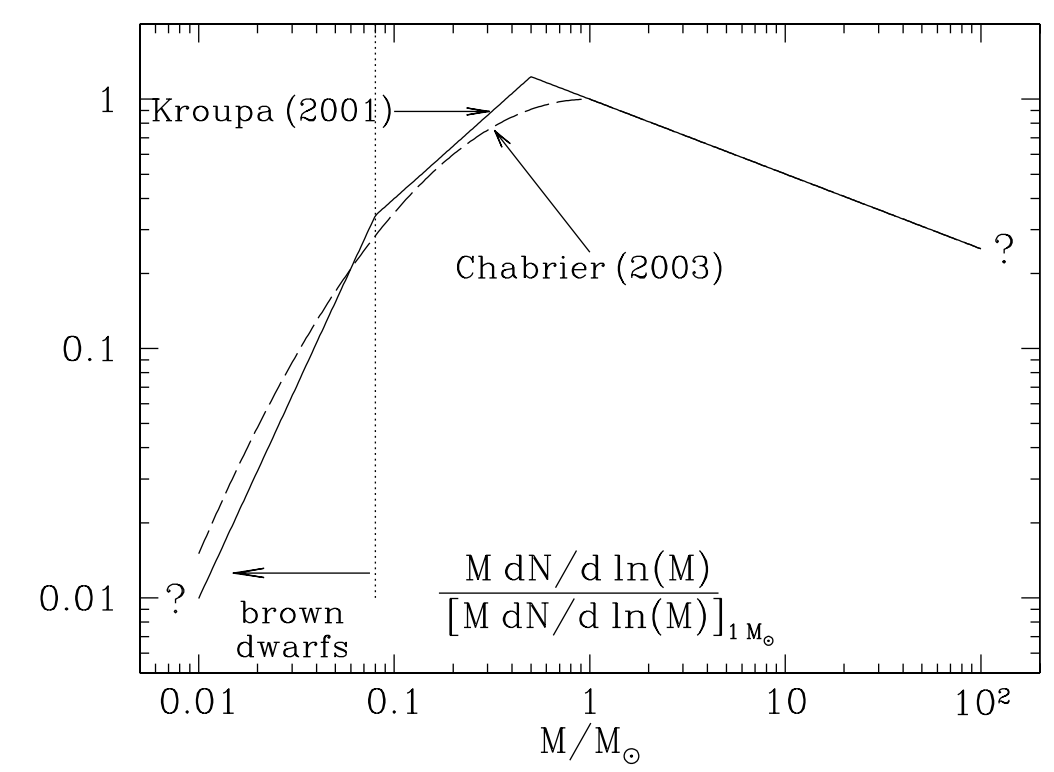
\includegraphics[width=10cm]{figures/KroupaChabrier.png}}
\end{figure}

{\noindent}Since the observable signatures for star formation are obtained only from massive stars, their formation rate needs to be extrapolated to lower masses to obtain the full SFR by assuming an IMF. Typically, a Salpeter-IMF is chosen between $0.1\,M_\odot\leq M\leq 100\,M_\odot$. However, there are clear indications that the IMF may be flatter for $M\lesssim1\,M_\odot$ than described by the Salpeter law, and several descriptions for such modified IMFs have been developed over the years, mainly based on observations and interpretation of star-forming regions in our MW or in nearby galaxies. The total stellar mass, obtained by integration over the IMF, is up to a factor of $\sim2$ lower in these modified IMFs than for the Salpeter IMF. Thus, this factor provides a characteristic uncertainty in the determination of the SFR from observations; a similar, though somewhat smaller uncertainty applies to the stellar mass density whose estimation also is mainly based on the more massive stars of a galaxy which dominate the luminosity. Furthermore, the IMF need not be universal, but may in principle vary between different environments, or depend on the metallicity of the gas from which stars are formed. Whereas there has not yet been unambiguous evidence for variations of the IMF, this possibility must always be taken into account.

\begin{table}[t]
    \centering
    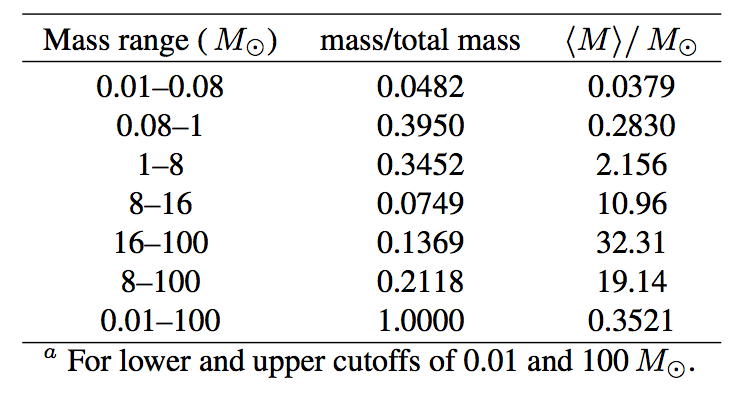
\includegraphics[width=10cm]{figures/ChabrierTable.png}
    \caption{\footnotesize{Some Properties of the Chabrier (2003) IMF$^a$. Table taken from Draine (2011).}}
    \label{table:chabrier}
\end{table}

{\noindent}As with theoretical models of the star formation rate, there is at present no completely satisfactory theory for the origin of the IMF, just different ideas that do better or worse at various aspects of the problem. To recall, the things we would really like to explain most are (1) the slope of the power-law at high masses, and (2) the location of the peak mass. We would also like to explain the little-to-zero variation in these quantities with galactic environment. Furthermore, we would like to explain the origin of the distribution of binary properties.

{\noindent}\textbf{The power-law tail}: Let us begin by considering the power-law tail at high masses, $\mathrm{d}N/\mathrm{d}M\propto M^{-\alpha}$ with $\alpha\approx2.3$. There are two main classes of theories for how this power-law tail is set: competitive accretion, and turbulence. Both are scale-free processes that could plausibly produce a power-law distribution of masses comparable to what is observed.

{\noindent}\textit{Competitive accretion}: One hypothesis for how to produce a power-law mass distribution is to consider what will happen in a region where a bunch of small ``seed'' stars are formed, but then begin to accrete at a rate that is a function of their current mass. Quantitatively, and for simplicity, suppose that every star accretes at a rate proportional to some power of its current mass, i.e.,

\begin{align*}
    \frac{dM}{dt} \propto M^\eta ~ [{\rm M_\odot\,yr^{-1}}].
\end{align*}

{\noindent}If we start with a mass $M_0$ and accretion rate $\dot{M}_0$ at time $t_0$, this ODE is easy to solve for the mass at later times. We get

\begin{equation*}
M(t) = M_o
\left\{
\begin{aligned}
[1-(\eta-1)\tau]^{1/(1-\eta)} ~ [{\rm M_\odot}], ~~~~~& \mathrm{if}\,\eta\neq1 \\
\exp(\tau) ~ [{\rm M_\odot}], ~~~~~& \mathrm{if}\,\eta=1
\end{aligned}
\right.
,
\end{equation*}

{\noindent}where $\tau=t/(M_0/\dot{M}_0)$ is the time measured in units of the initial mass-doubling time. The case for $\eta=1$ is the usual exponential growth, and the case for $\eta>1$ is even faster, running away to infinite mass in a finite amount of time $\tau=1/(\eta-1)$.

{\noindent}Now suppose that we start with a collection of stars that all begin at mass $M_0$, but have slightly different values of $\tau$ at which they stop growing, corresponding either to growth stopping at different physical times from one star to another, to stars stopping at the same time but having slightly different initial accretion rates $\dot{M}_0$, or some combination of both. What will the mass distribution of the resulting population be? If $dN/d\tau$ is the distribution of stopping times, then we will have

\begin{align*}
    \frac{dN}{d\tau} \propto \frac{dN/d\tau}{dM/\tau}M(\tau)^{-\eta}\frac{dN}{d\tau} ~ [{\rm dimensionless}].
\end{align*}

{\noindent}Thus the final distribution of masses will be a power-law in mass, with index $-\eta$, going from $M(\tau_\mathrm{min})$ to $M(\tau_\mathrm{max})$. Thus a power-law distribution naturally results.

{\noindent}The index of this power-law will depend on the index of the accretion law, $\eta$. What should this be? In the case of a point mass accreting from a uniform, infinite medium at rest, the accretion rate onto a point mass was worked out by Hoyle; Bondi generalized to the case of a moving medium. In either case, the accretion rate scales as $\dot{M}\propto M^2$, so if this process describes how stars form, then the expected mass distribution should follow $dN/dM\propto M^{-2}$, not so far from the actual slope of $-2.3$ that we observe. A number of authors have argued that this difference can be made up by considering the effects of a crowded environment, where the feeding regions of smaller stars get tidally truncated, and thus the growth law winds up begin somewhat steeper than $\dot{M}\propto M^2$.

{\noindent}This is an extremely simple model, requiring no physics but hydrodynamics and gravity, and thus it is easy to simulate. Simulations done based on this model do sometimes return a mass distribution that looks much like the IMF, as illustrated in Figure \ref{fig:imf}. However, this appears to depend on the choice of initial conditions. Generally speaking, one gets about the right IMF if one stars with something with a viral ratio $\alpha_\mathrm{vir}\sim1$ and no initial density structure, just velocities. Simulations that start with either super-virial or sub-virial initial conditions, or that begin with turbulent density structures, do not appear to grow as predicted by competitive accretion.

\begin{figure}[t]
    \floatbox[{\capbeside\thisfloatsetup{capbesideposition={right,top},capbesidewidth=4cm}}]{figure}[\FBwidth]
    {\caption{\footnotesize{The IMF measured in a simulation of the collapse of a $500\,{\rm M_\odot}$ initially uniform density cloud (Bate, 2009a). The single-hatched histogram shows all objects in the simulation, while the double-hatched one shows objects that have stopped accreting. Figure taken from Draine (2011).}}
    \label{fig:imf}}
    {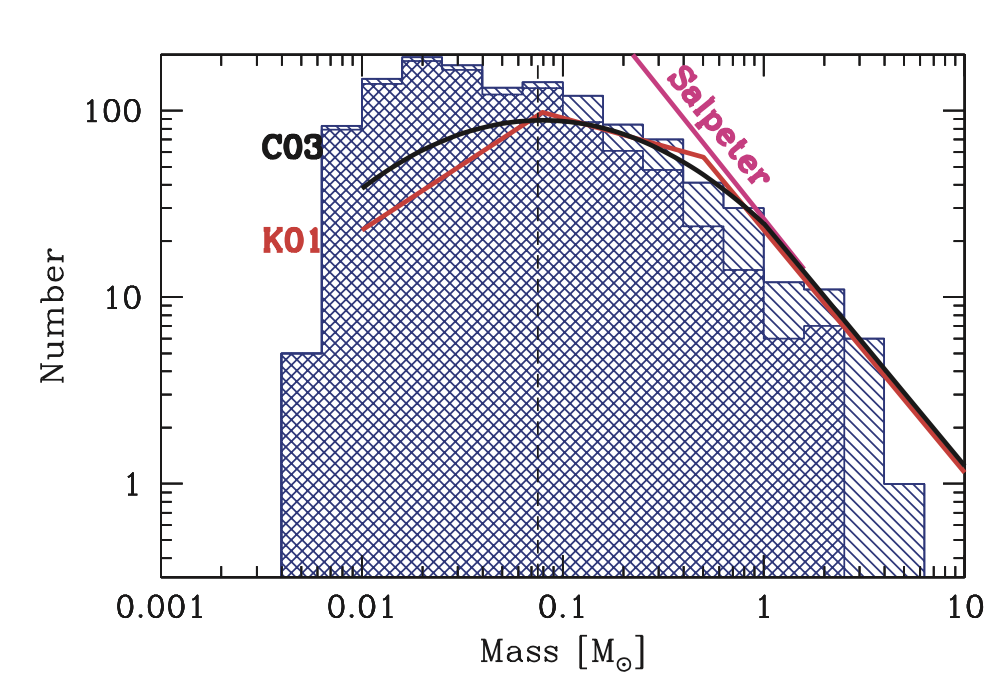
\includegraphics[width=12cm]{figures/IMF.png}}
\end{figure}

{\noindent}Another potential problem with this model is that it only seems to work in environments where there is no substantial feedback to drive the turbulence or eject the gas. In simulations where this is not true, there appears to be no competitive accretion. The key issue is that competitive accretion seems to require a global collapse where all the stars fall together into a region where they can compete, and this is hard to accomplish in the presence of feedback.

{\noindent}\textit{Turbulent fragmentation}: A second class of models for the origin of the power-law slope is based on the physics of turbulence. The first of these models was proposed by Padoan et al. (1997), and there have been numerous refinements since. The basic assumption in the turbulence models is that the process of shocks repeatedly passing through an isothermal medium leads to a broad range of density distributions, and that stars form wherever a local region happens to be pushed to the point where it becomes self-gravitating. We then proceed as follows. Suppose we consider the density field smoothed on some size scale $\ell$. The mass of an object of density $\rho$ in this smoothed field is

\begin{align*}
    M \sim \rho\ell^3 ~ [{\rm M_\odot}],
\end{align*}

{\noindent}and the total mass of objects with characteristic density between $\rho$
and $\rho+d\rho$ is

\begin{align*}
    dM_\mathrm{tot} \sim \rho p(\rho)d\rho ~ [{\rm M_\odot}],
\end{align*}

{\noindent}where $p(\rho)$ is the density PDF. Then the total number of objects in the mass range from $M$ to $M+dM$ on size scale $\ell$ can be obtained just by dividing the total mass of objects at a given density by the mass per object, and integrating over the density PDF on that size scale,

\begin{align*}
    \frac{dN_\ell}{dM} = \frac{dM_\mathrm{tot}}{M} \sim \ell^{-3} \int p(\rho)d\rho ~ [{\rm dimensionless}].
\end{align*}

{\noindent}Not all of these structures will be bound. To filter out the ones that are, we can impose a density threshold. We assert that an object will be bound only if its gravitational energy exceeds its kinetic energy, that is, only if the density exceeds a critical value given by

\begin{align*}
    \frac{GM^2}{\ell} \sim M\sigma_v(\ell)^2 ~ [{\rm J}] ~~~~~ \Rightarrow ~~~~~ \rho_\mathrm{crit} \sim \frac{\sigma_v(\ell)^2}{G\ell^2} ~ [{\rm g\,cm^{-3}}],
\end{align*}

{\noindent}where $\sigma_v(\ell)$ is the velocity dispersion on size scale $\ell$, which we take from the linewidth-size relation, $\sigma_v(\ell) = c_s\sqrt{(\ell/\ell_s)}$. Thus we have a critical density

\begin{align*}
    \rho_\mathrm{crit} \sim \frac{c_s^2}{G\ell_s\ell} ~ [{\rm g\,cm^{-3}}],
\end{align*}

{\noindent}and this forms a lower limit on the integral.

{\noindent}There are two more steps in the argument. One is simple: just integrate over all length scales to get the total number of objects. That is, 

\begin{align*}
    \frac{dN}{dM} \propto \frac{dN_\ell}{dM}d\ell ~ [{\rm M_\odot^{-1}}]. 
\end{align*}

{\noindent}The second is that we must know the functional form of $p(\rho)$ for the smoothed density PDF. One can get this in a couple of different ways, but there isn't a fully rigorous calculation. Hopkins get it by assuming that the PDF is log-normal smoothed on all scales with a dispersion that is an integral over the dispersions on smaller scales. Hennebelle \& Chabrier, in their model, assume that the density power spectrum is a power-law, and derive the density PDF from that. The assumptions yield similar but not identical results. 

{\noindent}At this point we will simply assert that one can evaluate all the integrals to get an IMF. The result clearly depends only on two dimensional quantities: the sound speed $c_s$ and the sonic length $\ell_s$. However, at masses much greater than the sonic mass $M_s \approx c_s^2\ell_s/G$, the result is close to a power-law with approximately the right index. Figure \ref{fig:imfmodel} shows an example prediction.

\begin{figure}[t]
    \floatbox[{\capbeside\thisfloatsetup{capbesideposition={right,top},capbesidewidth=4cm}}]{figure}[\FBwidth]
    {\caption{\footnotesize{The IMF predicted by an analytic model of turbulent fragmentation by Hopkins (2012). Figure taken from Draine (2011).}}
    \label{fig:imfmodel}}
    {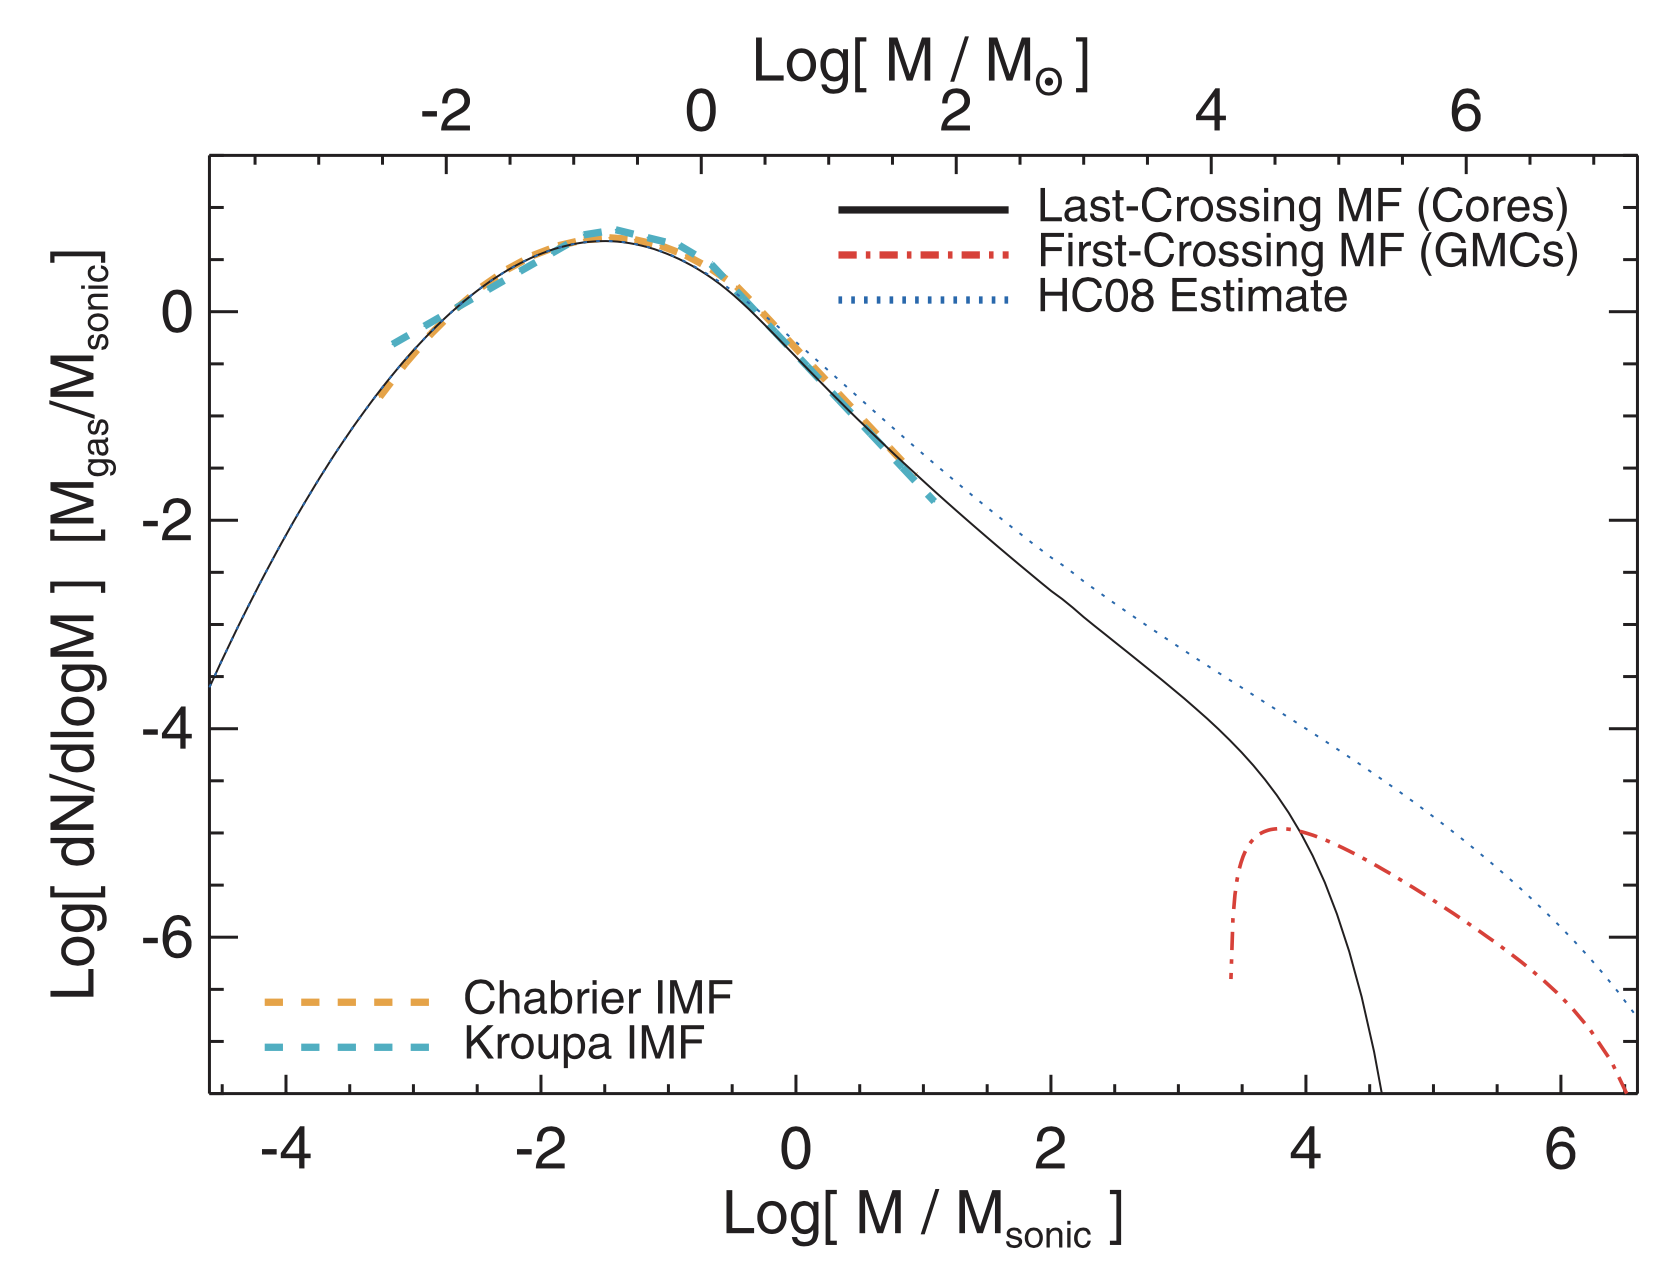
\includegraphics[width=12cm]{figures/IMFmodel.png}}
\end{figure}

{\noindent}As with the competitive accretion model, this hypothesis encounters certain difficulties. First, there is the technical problem that the choice of smoothed density PDF estimate is not at all rigorous, and there are noticeable differences between on how the choice is made. Second, the dependence on the sonic length is potentially problematic, because real molecular clouds do not really have constant sonic lengths. Regions of massive star formation are observed to be systematically more turbulent.

{\noindent}Third, the theory does not address the question of why gravitationally-bound regions don’t sub-fragment as they collapse. Finally, the model has trouble explaining the IMF peak, for the exact same reason as competitive accretion.

{\noindent}\textbf{The peak of the IMF}: A power-law is scale-free, but the peak has a definite mass scale. This mass scale is one basic observable that any theory of star formation must be able to predict. This immediately tells us something about the physical processes that must be involved. We have thus far thought of molecular clouds as consisting mostly of isothermal, turbulent, magnetized, self-gravitating gas. However, we can show that there must be additional processes beyond these at work in setting a peak mass.

{\noindent}We can see this in a few ways. First we'll demonstrate it in a more intuitive but not rigorous manner, and then we can demonstrate it rigorously. The intuitive arguments is as follows. In the system we have described, there are four energies in the problem: thermal energy, bulk kinetic energy, magnetic energy, and gravitational potential energy. From these energies we can define three dimensionless ratios, and the behavior of the system will be determined by these three ratios. As an example, we might define

\begin{align*}
    \mathcal{M}=\frac{\sigma_v}{c_s} ~ [{\rm dimensionless}] ~~~~~ \beta=\frac{8\pi\rho c_c^2}{B^2} ~ [{\rm dimensionless}] ~~~~~ n_J=\frac{\rho L^2}{c_s^3/\sqrt{G^3\rho}} ~ [{\rm dimensionless}].
\end{align*}

{\noindent}The ratios describe the ratio of kinetic to thermal energy, the ratio of thermal to magnetic energy, and the ratio of thermal to gravitational energy. (This last quantity is called the Jeans number: it is the ratio of the cloud mass to the Jeans mass.) Other ratios can be derived from these, e.g., the Alfv\'enic Mach number $\mathcal{M}=\mathcal{M}\sqrt{\beta/2}$ is the ratio of the kinetic to magnetic energy.

{\noindent}Now notice the scalings of these numbers with density $\rho$, velocity dispersion $\sigma_v$, magnetic field strength $B$, and length scale $L$:

\begin{align*}
    \mathcal{M}\propto\sigma_v ~ [{\rm dimensionless}] ~~~~~ \beta\propto\rho B^{-2} ~ [{\rm dimensionless}] ~~~~~ n_J\propto\rho^{3/2}L^3 ~ [{\rm dimensionless}].
\end{align*}

{\noindent}Notice that if we scale the problem by $\rho\rightarrow x\rho$, $L\rightarrow x^{-1/2}L$, $B\rightarrow x^{1/2}B$, all of these dimensionless numbers remain fixed. Thus the behavior of two systems, one with density a factor of $x$ times larger than the other one, length a factor of $x^{-1/2}$ smaller, and magnetic field a factor of $x^{1/2}$ stronger, are simply rescaled versions of one another. If the first system fragments to make a star out of a certain part of its gas, the second system will too. Notice, however, that the masses of those stars will not be the same! The first star will have a mass that scales as $\rho L^3$, while the second will have a mass that scales as $(x\rho)(x^{-1/2}L)^3=x^{-1/2}\rho L^3$.

{\noindent}We learn from this an important lesson: isothermal gas is scale-free. If we have a model involving only isothermal gas with turbulence, gravity, and magnetic fields, and this model produces stars of a given mass $M_*$, then we can rescale the system to obtain an arbitrarily different mass. Explaining the IMF peak requires appealing to some physics beyond that of isothermal, magnetized turbulence plus self-gravity. This immediately shows that the competitive accretion and turbulence theories we outlined to explain the power-law tail of the IMF cannot be adequate to explaining the IMF peak, at least not by themselves. Something must be added, and models for the origin of the IMF peak can be broadly classified based on what extra physics they choose to add.

{\noindent}\textbf{The outer scale of turbulence}: One option is hypothesize that the IMF is set at the outer scale of the turbulence, where the molecular clouds join to the atomic ISM (in a galaxy like the MW), or on sizes of the galactic scale-height (for a molecule-dominated galaxy). Something in this outer scale picks out the characteristic mass of stars at the IMF peak.

{\noindent}This hypothesis comes in two flavors. The simplest is that characteristic mass is simply set by the Jeans mass at the mean density of the cloud, so that

\begin{align*}
    M_\mathrm{peak} \propto \frac{c_s^3}{\sqrt{G^3\bar{\rho}}} ~ [{\rm M_\odot}].
\end{align*}

{\noindent}While simple, this hypothesis immediately encounters problems. Molecular clouds have about the same temperature everywhere, but they do not all have the same density -- indeed, the density should vary with cloud mass as $M^{1/2}$. Thus at face value this hypothesis would seem to predict a factor of $\sim3$ difference in characteristic peak mass between $10^4$ and $10^6\,{\rm M_\odot}$ clouds in the MW. This is pretty hard to reconcile with observations. The problem is even worse if we think about other galaxies, where the range of density variation is much greater and thus the predicted IMF variation is too. One can hope for a convenient cancellation, whereby an increase in the density is balanced by an increase in temperature, but this seems to require a coincidence.

{\noindent}A somewhat more refined hypothesis, which is adopted by all the turbulence models, is that the IMF peak is set by the sound speed and the normalization of the linewidth-size relation. As discussed above, in the turbulence models the only dimensional free parameters are $c_s$ and $\ell_s$, and from them one can derive a mass in only one way:

\begin{align*}
    M_\mathrm{peak} \propto \frac{c_s^2\ell_s}{G} ~ [{\rm M_\odot}].
\end{align*}

{\noindent}Hopkins calls this quantity the sonic mass, but it’s the same thing as the characteristic masses in the other models.

{\noindent}This value can be expressed in a few ways. Suppose that we have a cloud of characteristic mass $M$ and radius $R$. We can write the velocity dispersion in terms of the virial parameter:

\begin{align*}
    \alpha_\mathrm{vir} \sim \frac{\sigma_vR}{GM} ~ [{\rm dimensionless}].
\end{align*}

{\noindent}This is the velocity dispersion on the outer scale of the cloud, so we can also define the Mach number on this scale as

\begin{align*}
    \mathcal{M} = \frac{\sigma_v}{c_s} \sim \sqrt{\alpha_\mathrm{vir}\frac{GM}{Rc_s^2}} ~ [{\rm dimensionless}].
\end{align*}

{\noindent}The sonic length is just the length scale at which $\mathcal{M}\sim1$, so if the velocity dispersion scales with $\ell^{1/2}$, then we have

\begin{align*}
    \ell_s \sim \frac{R}{\mathcal{M}^2} \sim \frac{c_s^2}{\alpha_\mathrm{vir}G\Sigma} ~ [{\rm pc}].
\end{align*}

{\noindent}Substituting this in, we have

\begin{align*}
    M_\mathrm{peak} \sim \frac{c_s^4}{\alpha_\mathrm{vir}G^2\Sigma} ~ [{\rm M_\odot}],
\end{align*}

{\noindent}and thus the peak mass simply depends on the surface density of the cloud. We can obtain another equivalent expression by noticing that

\begin{align*}
    \frac{M_J}{\mathcal{M}} \sim \frac{c_s^3}{\sqrt{G^3\bar{\rho}}} \sqrt{\frac{Rc_s^2}{\alpha_\mathrm{vir}GM}} \sim \frac{c_s^4}{\alpha_\mathrm{vir}G^2\Sigma} \sim M_\mathrm{peak} ~ [{\rm M_\odot}].
\end{align*}

{\noindent}Thus, up to a factor of order unity, this hypothesis is also equivalent to assuming that the characteristic mass is simply the Jeans mass divided by the Mach number.

{\noindent}An appealing aspect of this argument is that it naturally explains why molecular clouds in the MW all make stars at about the same mass. A less appealing result is that it would seem to predict that the masses could be quite different in regions of different surface density, and we observe that there are star-forming regions where $\Sigma$ is indeed much higher than the mean of the MW GMCs. This is doubly-true if we extend our range to extragalactic environments. One can hope that this will cancel because the temperature will be higher and thus $c_s$ will increase, but this again seems to depend on a lucky cancellation, and there is no a priori reason why it should.

{\noindent}\textbf{Non-isothermal fragmentation}: The alternative to breaking the isothermality at the outer scale of the turbulence is to relax the assumption that the gas is isothermal on small scales. This has the advantage that it avoids any ambiguity about what constitutes the surface density or linewidth-size relation normalization for a ``cloud''.

{\noindent}The earliest versions of these models were proposed by Larson (2005), and followed up by Jappsen et al. (2005). The basic idea of these models is that the gas in star-forming clouds is only approximately isothermal. Instead, there are small deviations from isothermality, which can pick out preferred mass scales. There are two places where significant deviations from isothermality are expected (Figure \ref{fig:sf_tvsrho}).

\begin{figure}[t]
    \floatbox[{\capbeside\thisfloatsetup{capbesideposition={right,top},capbesidewidth=4cm}}]{figure}[\FBwidth]
    {\caption{\footnotesize{Temperature versus density found in a one-dimensional calculation of the collapse of a $1\,{\rm M_\odot}$ gas cloud, at the moment immediately before a central protostar forms. Figure taken from Draine (2011).}}
    \label{fig:sf_tvsrho}}
    {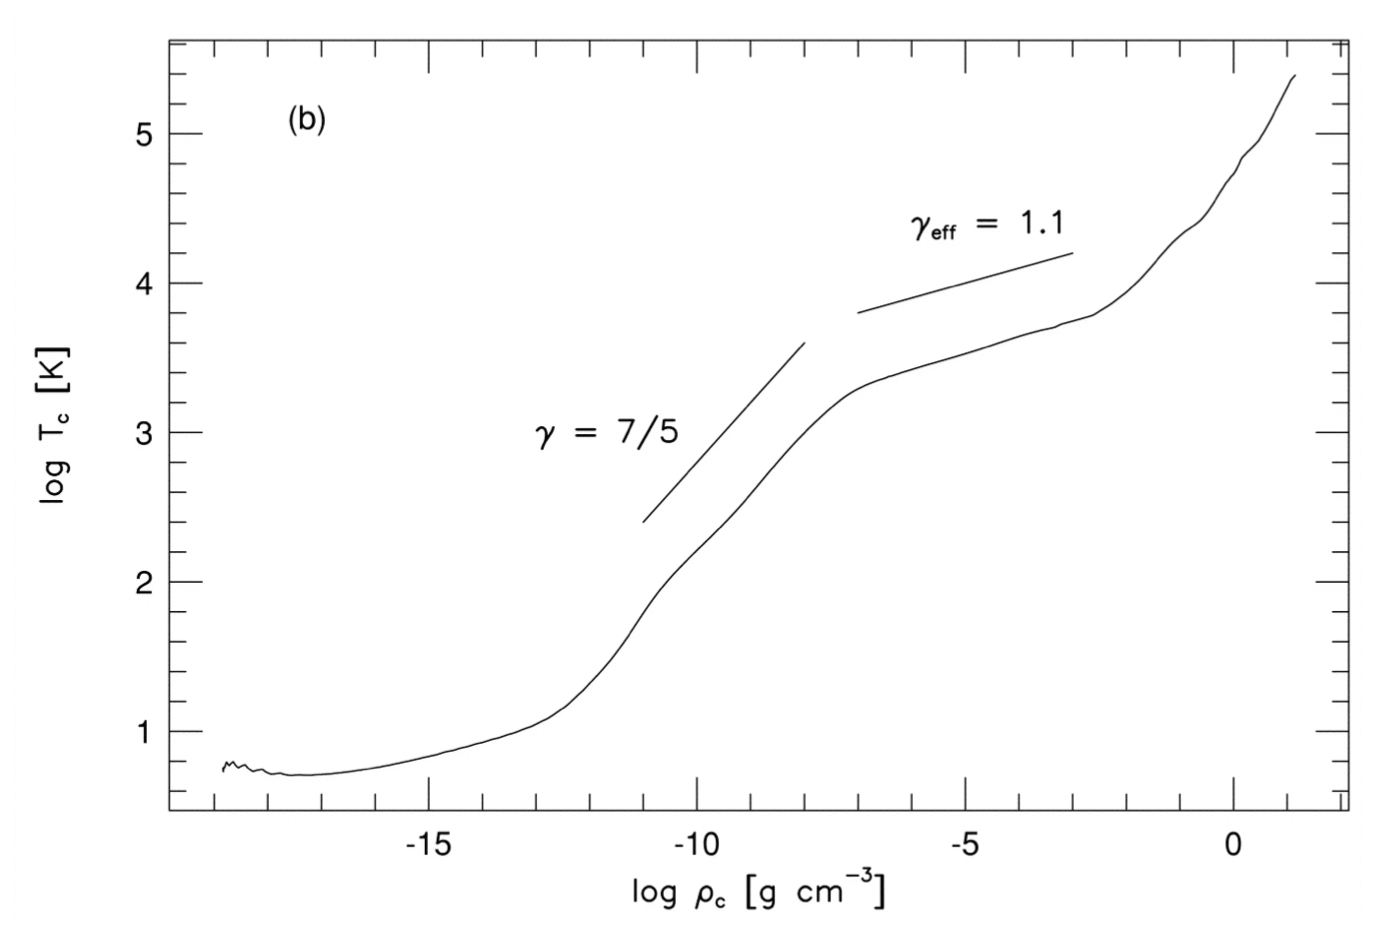
\includegraphics[width=12cm]{figures/SF_TvsRho.png}}
\end{figure}

{\noindent}At low density the main heating source is cosmic rays and UV photons, both of which produce a constant heating rate per nucleus if attenuation is not significant. This is because the flux of CRs and UV photons is about constant, and the rate of energy deposition is just proportional to the number of target atoms or dust grains for them to interact with. Cooling is primarily by lines, either of CO once the gas is mostly molecular, or of C$_\mathrm{II}$ or O where it is significantly atomic.

{\noindent}In both cases, at low density the gas is slightly below the critical density of the line, so the cooling rate per nucleus or per molecule is an increasing function of density. Since heating per nucleus is constant but cooling per nucleus increases, the equilibrium temperature decreases with density. As one goes to higher density and passes the CO critical density this effect ceases. At that point one generally starts to reach densities such that shielding against UV photons is significant, so the heating rate goes down and thus the temperature continues to drop with density.

{\noindent}This begins to change at a density of around $10^{18}\,{\rm g\,cm^{-3}}$, $n\sim10^5--10^6\,{\rm cm^{-3}}$. By this point the gas and dust have been thermally well-coupled by collisions, and the molecular lines are extremely optically thick, so dust is the main thermostat. As long as the gas is optically thin to thermal dust emission, which it is at these densities, the dust cooling rate per molecule is fixed, since the cooling rate just depends on the number of dust grains. Heating at these densities comes primarily from compression as the gas collapses, i.e., it is just $P{\rm d}V$ work. If the compression were at a constant rate, the heating rate per molecule would be constant. However, the free-fall time decreases with density, so the collapse rate and thus the heating rate per molecule increase with density. The combination of fixed cooling rate and increasing heating rate causes the temperature to begin rising with density. At still higher densities, $10^{13}\,{\rm g\,cm^{-3}}$, the gas becomes optically thick to dust thermal emission. At this point the gas simply acts adiabatically, with all the $PdV$ work being retained, so the heating rate with density rises again.

{\noindent}Larson (2005) pointed out that deviations from isothermality are particularly significant for filamentary structures, which dominate in turbulent flows. It is possible to show that a filament cannot go into runaway collapse if $T$ varies with $\rho$ to a positive number, while it can collapse if $T$ varies as $\rho$ to a negative number. This suggests that filaments will collapse indefinitely in the low-density regime, but that their collapse will then halt around $10^{18}\,{\rm g\,cm^{-3}}$, forcing them to break up into spheres in order to collapse further. The upshot of all these arguments is that the Jeans or Bonnor-Ebert mass one should be using to estimate the peak of the stellar mass spectrum is the one corresponding to the point where there is a changeover from sub-isothermal to super-isothermal.

{\noindent}In other words, the $\rho$ and $T$ that should be used to evaluate $M_J$ or $M_{BE}$ are the values at that transition point. Larson proposes an approximate equation of state to represent the first break in the EOS: Combining all these effects, Larson (2005) proposed a single simple equation of state

\begin{equation*}
T =
\left\{
\begin{aligned}
4.4\rho_{18}^{-0.27} ~ [{\rm K}], ~~~~~& \mathrm{if}\,\rho_{18}<1 \\
4.4\rho_{18}^{0.07} ~ [{\rm K}], ~~~~~& \mathrm{if}\,\rho_{18}\geq1
\end{aligned}
\right.
,
\end{equation*}

{\noindent}where $\rho_{18}=\rho/(10^{18}\,{\rm g\,cm^{-33}})$. Conveniently enough, the Bonnor-Ebert mass at the minimum temperature here is $M_{BE}=0.067\,{\rm M_\odot}$, which is not too far off from the observed peak of the IMF at $M_\mathrm{peak}=0.2\,{\rm M_\odot}$. (The mass at the second break is a bit less promising. At $\rho=10^{13}\,{\rm g\,cm^{13}}$ and $T=10\,{\rm K}$, we have $M_{BE}=7\times10^{-4}\,{\rm M_\odot}$).

{\noindent}Simulations done adopting this proposed equation of state seem to verify the conjecture that the characteristic fragment mass does depend critically on the break on the EOS (Figure \ref{fig:imfmodels}).

\begin{figure}[t!]
    \centering
    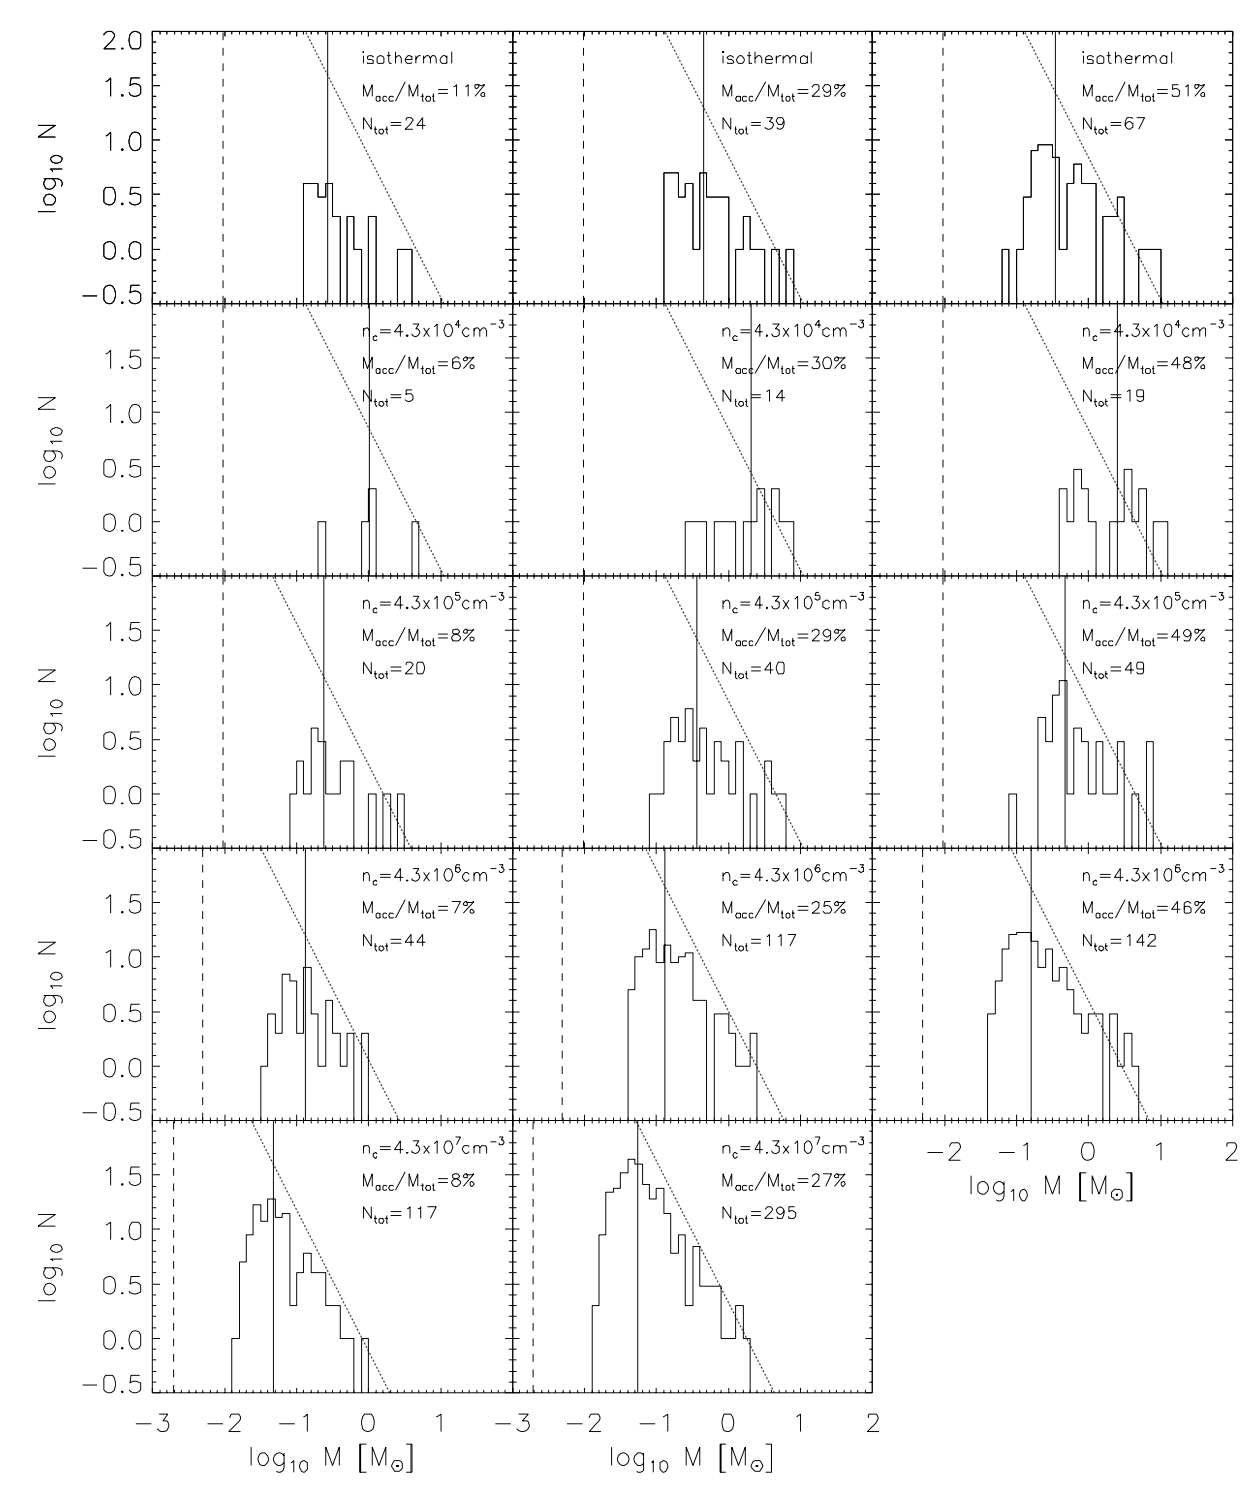
\includegraphics[width=16cm]{figures/IMFmodels.png}
    \caption{\footnotesize{Measured stellar mass distributions in a series of simulations of turbulent fragmentation using non-isothermal EOSs. Each row shows a single simulation, measured at a series of times, characterized by a particular mass in stars as indicated in each panel. Different rows use different EOSs, with the vertical line in each panel indicating the Jeans mass evaluated at the temperature minimum of the equation of state. Histograms show the mass distributions measured for the stars. Figure taken from Draine (2011).}}
    \label{fig:imfmodels}
\end{figure}

{\noindent}While this is a very interesting result, there are two problems. First, the proposed break in the EOS occurs at $n=4\times10^5\,{\rm cm^{-3}}$. This is a fairly high density in a low mass star-forming region, but it is actually quite a low density in more typical, massive star-forming regions. For example, the Orion Nebula cluster (ONC) now consists of $4600\,{M_\odot}$ of stars in a radius of $0.8\,{\rm pc}$, giving a mean density $n=3.7\times10^4\,{\rm cm^{-3}}$. Since the SF efficiency was less than unity and the cluster is probably expanding due to mass loss, the mean density was almost certainly higher while the stars were still forming. Moreover, recall that, in a turbulent medium, the bulk of the mass is at densities above the volumetric mean density. The upshot of all this is that almost all the gas in Orion was probably over Larson (2005)'s break density while the stars were forming. Since Orion managed to form a normal IMF, it's not clear how the break temperature could be relevant.

{\noindent}A second problem is that, in dense regions like the ONC, the simple model proposed by Larson (2005) is a very bad representation of the true temperature structure, because it ignores the effects of radiative feedback from stars. In dense regions the stars that form will heat the gas around them, raising the temperature. Figure \ref{fig:tvsrho_feedback} shows the density-temperature distribution of gas in simulations that include radiative transfer, and that have conditions chosen to be similar to those of the ONC.

\begin{figure}[t]
    \centering
    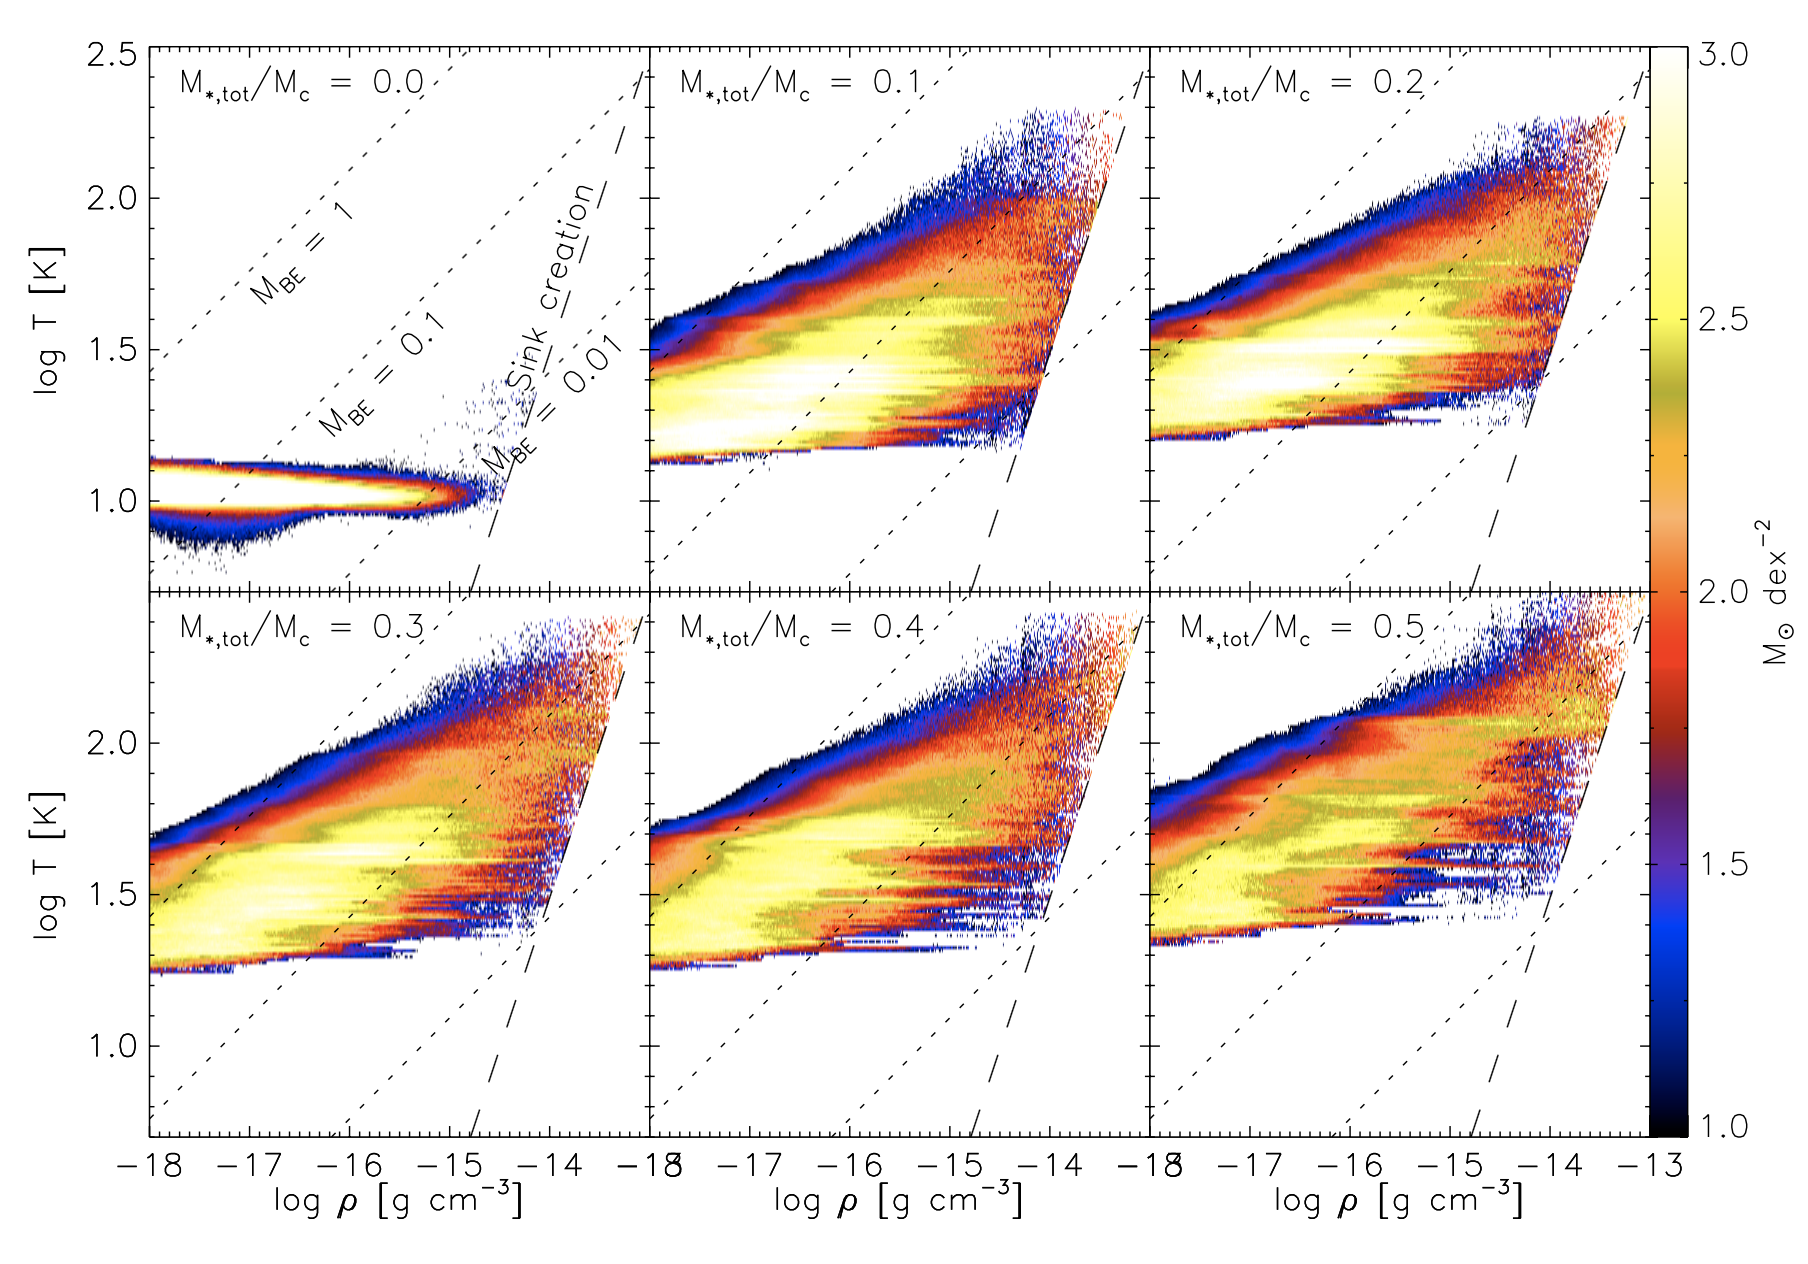
\includegraphics[width=16cm]{figures/TvsRho_feeback.png}
    \caption{\footnotesize{Density-temperature distributions measured from a simulation of the formation of an ONC-like star cluster, including radiative transfer and stellar feedback (Krumholz et al., 2011a). The panels show the distribution at different times in the simulation, characterized by the fraction of mass that has been turned into stars. Doted lines show lines of constant Bonnor-Ebert mass (in ${\rm M_\odot}$), while dashed lines show the threshold for sink particle formation in the simulation. Histograms show the mass distributions measured for the stars. Figure taken from Draine (2011).}}
    \label{fig:tvsrho_feedback}
\end{figure}

{\noindent}These two observations suggest that one can build a model for the IMF around radiative feedback. There are a few numerical and analytic papers that attempt to do so, including Bate (2009b, 2012), Krumholz (2011), and Krumholz et al. (2012b). The central idea for these models is that radiative feedback shuts off fragmentation at a characteristic mass scale that sets the peak of the IMF.

{\noindent}The basic idea is as follows. Suppose that we form a first, small protostellar that radiates at a rate $L$. The temperature of the material at a distance $R$ from it, assuming the gas is optically thick, will be roughly

\begin{align*}
    L\approx 4\pi R^2\sigma T^4 ~ [{\rm erg\,s^{-1}}].
\end{align*}

{\noindent}Now let us compute the Bonnor-Ebert mass using the temperature $T$:

\begin{align*}
    M_{BE} \approx \frac{c_s^3}{\sqrt{G^3\rho}} = \sqrt{\left(\frac{k_BT}{\mu m_HG}\right)^3\frac{1}{\rho}},
\end{align*}

{\noindent}where $\mu=2.33$ is the mean particle mass, and we are omitting the factor of $1.18$ for simplicity. Note that $M_{BE}$ here is a function of $R$. At small $R$, $T$ is large and thus $M_{BE}$ is large, while at larger distances the gas is cooler and $M_{BE}$ falls.

{\noindent}Now let us compare this mass to the mass enclosed within the radius $R$, which is $M=(4/3)\pi R^3\rho$. At small radii, $M_{BE}$ greatly exceeds the enclosed mass, while at large radii $M_{BE}$ is much less than the enclosed mass. A reasonable hypothesis is that fragmentation will be suppressed out to the point where $M\approx M_{BE}$. If we solve for the radius $R$ and mass $M$ at which this condition is met, we obtain

\begin{align*}
    M\approx \left(\frac{1}{36\pi}\right)^{1/10} \left(\frac{k_B}{G\mu m_H}\right)^{6/5} \left(\frac{L}{\sigma}\right)^{3/10} \rho^{-1/5} ~ [{\rm M_\odot}].
\end{align*}

{\noindent}To go further, we need to know the luminosity $L$. The good news is that the luminosity is dominated by accretion, and the energy produced by accretion is simply the accretion rate multiplied by a roughly fixed energy yield per unit mass. In other words, we can write

\begin{align*}
    L \approx \phi\dot{M} ~ [{\rm erg\,s^{-1}}].
\end{align*}

{\noindent}where $\phi=10^{14}\,{\rm erg\,g^{-1}}$, and can in fact be written in terms of fundamental constants. Taking this on faith for now, if we further assume that stars form over a time of order a free-fall time, then

\begin{align*}
    \dot{M}\approx M\sqrt{G\rho} ~ [{\rm M_\odot\,yr^{-1}}],
\end{align*}

{\noindent}and substituting this into the equation for $M$ above and solving gives

\begin{align*}
    M\approx \left(\frac{1}{36\pi}\right)^{1/7} \left(\frac{k_B}{G\mu m_H}\right)^{12/7} \left(\frac{\phi}{\sigma}\right)^{3/7} \rho^{-1/14} = 0.3\left(\frac{n}{100\,{\rm cm^{-3}}}\right)^{-1/14} ~ [{\rm M_\odot}],
\end{align*}

{\noindent}where $n=\rho/(\mu m_H)$. Thus we get a characteristic mass that is a good match to the IMF peak, and that depends only very, very weakling on the ambient density.

{\noindent}Simulations including radiation seem to support the idea that this effect can pick out a characteristic peak ISM mass. The main downside to this hypothesis is that it has little to say by itself about the power-law tail of the IMF. This is not so much a problem with the model as an omission, and a promising area of research seems to be joining a non-isothermal model such as this onto a turbulent fragmentation or competitive accretion model to explain the full IMF.

{\noindent}\textbf{Measuring the IMF}: There are two major strategies for measuring the IMF. One is to use direct star counts in regions where we can resolve individual stars. The other is to use integrated light from more distant regions where we cannot. The former itself contains two different methods, one using field stars and the other using young clusters.

{\noindent}\textit{Field stars (resolved stars)}: The first attempts to measure the IMF were by Salpeter (1955) (for those counting, nearly 5000 citations as of this writing), using stars in the Solar neighborhood, and the use of Solar neighborhood stars remains one of the main strategies for measuring the IMF today. Suppose that we want to measure the IMF of the field stars within some volume or angular region around the Sun. What steps must we carry out?

{\noindent}The first step is to construct a luminosity function for the stars in our survey volume in one or more photometric bands. This by itself is a non-trivial task, because we require absolute luminosities, which means we require distances. If we are carrying out a volume-limited instead of a flux-limited survey, we also require distances to determine if the target stars are within our survey volume.

{\noindent}The most accurate distances available are from parallax, but this presents a challenge. To measure the IMF, we require a sample of stars that extends down to the lowest masses we wish to measure. As one proceeds to lower masses, the stars very rapidly become dimmer, and as they become dimmer it becomes harder and harder to obtain parallax distances. For $\sim0.1\,{\rm M_\odot}$ stars, typical absolute V band magnitudes are $M_V\sim14$, and parallax catalogues at such magnitudes are only complete out to $\sim5-10\,{\rm pc}$. A survey of this volume only contains $200-300$ stars and brown dwarfs, and this sample size presents a fundamental limit on how well the IMF can be measured. If one reduces the mass range being studied, parallax catalogues can go out somewhat further, but then one is trading off sample size against the mass range that the study can probe. Hopefully Gaia will improve this situation significantly.

{\noindent}For these reasons, more recent studies have tended to rely on less accurate spectroscopic or photometric distances. These introduce significant uncertainties in the luminosity function, but they are more than compensated for by the vastly larger number of stars available, which in the most recent studies can be $>10^6$. The general procedure for photometric distances is to construct color-magnitude (CMD) diagrams in one or more colors for Solar neighborhood stars using the limited sample of stars with measured parallax distances, perhaps aided by theoretical models. Each observed star with an unknown distance is then assigned an absolute magnitude based on its color and the CMD. The absolute magnitude plus the observed magnitude also gives a distance. The spectroscopic parallax method is analogous, except that one uses spectral type - magnitude diagrams (STMD) in place of color-magnitude ones to assign absolute magnitudes. This can be more accurate, but requires at least low resolution spectroscopy instead of simply photometry.

{\noindent}Once that procedure is done, one has in hand an absolute luminosity function, either over a defined volume or (more commonly) a defined absolute magnitude limit. The next step is to correct it for a series of biases. We will not go into the technical details of how the corrections are made, but it is worth going through the list just to understand the issues, and why this is not a trivial task:

\begin{itemize}
    \item \textbf{Metallicity bias}: The reference CMDs or STMDs used to assign absolute magnitudes are constructed from samples very close to the Sun with parallax distances. However, there is a known negative metallicity gradient with height above the galactic plane, so a survey going out to larger distances will have a lower average metallicity than the reference sample. This matters because stars with lower metallicity have higher effective temperature and earlier spectral type than stars of the same mass with lower metallicity. (They have slightly higher absolute luminosity as well, but this is a smaller effect.) As a result, if the CMD or STMD used to assign absolute magnitudes is constructed for Solar metallicity stars, but an actual star being observed is sub-Solar, then we will tend to assign too high an absolute luminosity based on the color, and, when comparing with the observed luminosity, too large a distance. We can correct for this bias if we know the vertical metallicity gradient of the galaxy.
    \item \textbf{Extinction bias}: The reference CMDs/STMDs are constructed for nearby stars, which are systematically less extincted than more distant stars because their light travels through less of the dusty galactic disk. Dust extinction reddens starlight, which causes the more distant stars to be assigned artificially red colors, and thus artificially low magnitudes. This in turn causes their absolute magnitudes and distances to be underestimated, moving stars from their true luminosities to lower values. These effects can be mitigated with knowledge of the shape of the dust extinction curve and estimates of how much extinction there is likely to be as a function of distance.
    \item \textbf{Malmquist bias}: There is some scatter in the magnitudes of stars at fixed color, both due to the intrinsic physical width of the main sequence (e.g., due to varying metallicity, age, stellar rotation) and due to measurement error. Thus at fixed color magnitudes can scatter up or down. Consider how this affects stars that are near the distance of magnitude limit for the survey: stars whose true magnitude should place them just outside the survey volume or flux limit will be artificially scatter into the survey if they scatter up but not if they scatter down, and those whose true magnitude should place them within the survey will be removed if they scatter to lower magnitude. This asymmetry means that, for stars near the distance or magnitude cutoff of the survey, the errors are not symmetric; they are much more likely to be in the direction of positive than negative flux. This effect is known as Malmquist bias. It can be corrected to the extent that one has a good idea of the size of the scatter in magnitude and understands the survey selection.
    \item \textbf{Binarity}: Many stars are members of binary systems, and all but the most distant of these will be unresolved in the observations and will be mistaken for a single star. This has a number of subtle effects, which we can think of in two limiting cases. If the binary is far from equal mass, say $M2/M1\sim0.3$ or less, then the colors and absolute magnitude will not be that different from those of the primary stuff. Thus the main effect is that we do not see the lower mass member of the system at all. We get a reasonable estimate for the properties of the primary, but we miss the secondary entirely, and therefore under-count the number of low luminosity stars. On the other hand, if the mass ratio $M2/M1\sim1$ then the main effect is that the color stays about the same, but using our CMD we assign the luminosity of a single star when the true luminosity is actually twice that. We therefore underestimate the distance, and artificially scatter things into the survey (if it is volume limited) or out of the survey (if it is luminosity limited). At intermediate mass ratios, we get a little of both effects. The means of correcting for this, if we have a reasonable estimate of the binary fraction of mass ratio distribution, to guess a true luminosity function, determine which stars are binaries, add them together as they would be added in observations, filter the resulting catalogue through the survey selection, and compare to the observed luminosity function. This procedure is then repeated, adjusting the guessed luminosity function, until the simulated observed luminosity function matches the actually observed one.
\end{itemize}

{\noindent}Once all these bias corrections are made, the result is a corrected luminosity function that (should) faithfully reproduce the actual luminosity function in the survey volume. Figure \ref{fig:lumfunc} shows an example of raw and corrected luminosity functions.

\begin{figure}[h!]
    \centering
    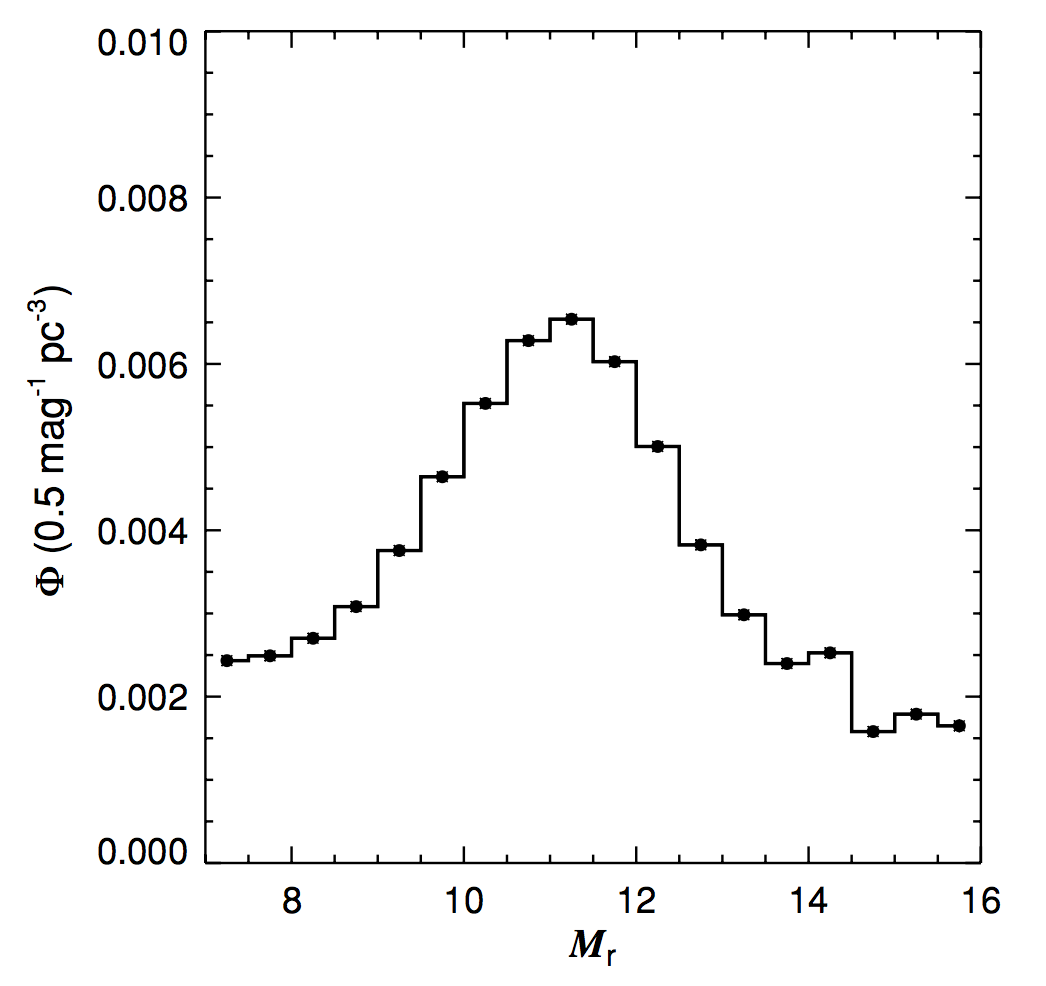
\includegraphics[width=7cm]{figures/lumfunc_before.png} 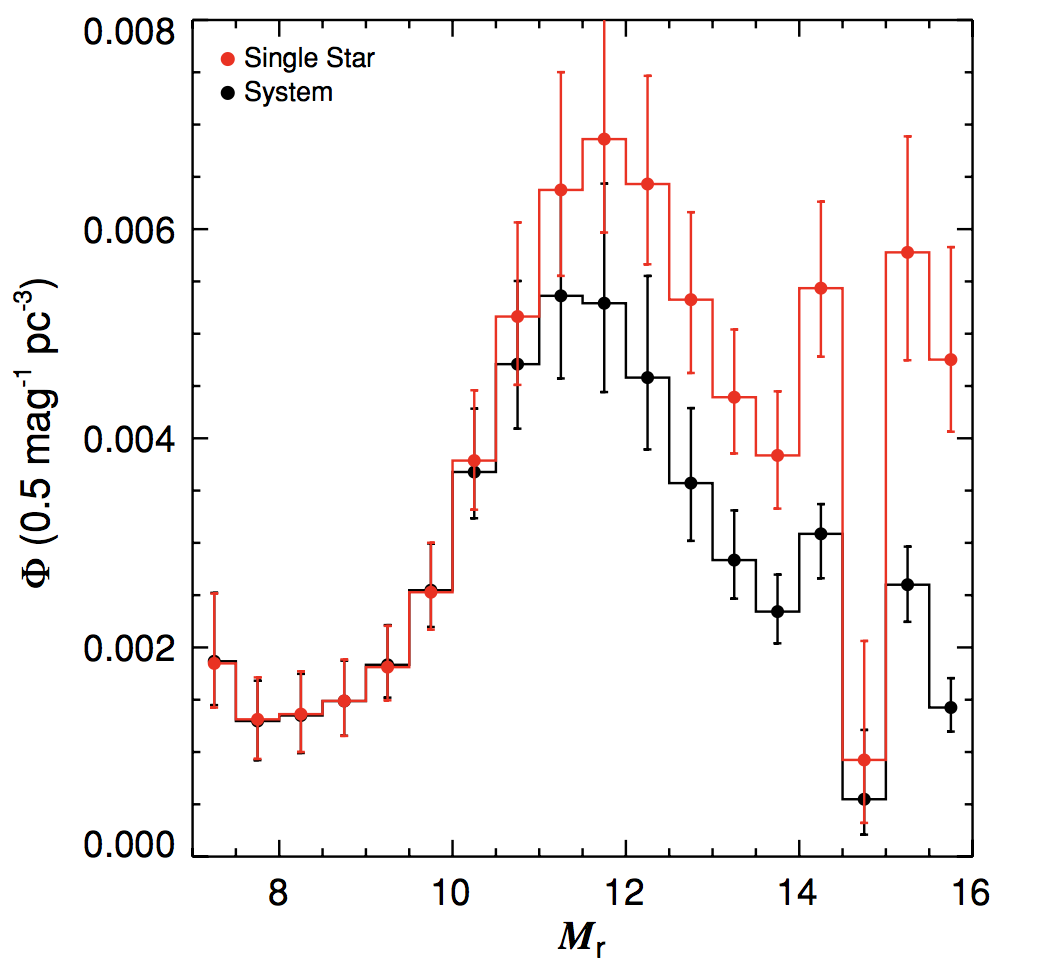
\includegraphics[width=7cm]{figures/lumfunc_after.png}
    \caption{\footnotesize{Luminosity function for MW stars before (left) and after (right) bias correction. Figure taken from Draine (2011).}}
    \label{fig:lumfunc}
\end{figure}

{\noindent}The next step is to convert the luminosity function into a mass function, which requires knowledge of the mass-magnitude relation (MMR) in whatever photometric band we have used for our luminosity function. This must either be determined by theoretical modeling, empirical calibration, or both. Particularly at the low-mass end, the theoretical models tend to have significant uncertainties arising from complex atmospheric chemistry that affects the optical and even NIR colours. For empirical calibrations, the data are only as good as the empirical mass determinations, which must come from orbit modeling. This requires the usual schemes for measuring stellar masses from orbits, e.g., binaries that are both spectroscopic and eclipsing, and thus have known inclinations, or visual binaries with measured radial velocities. 

{\noindent}As with the luminosity function, there are a number of possible biases because the stars are not uniform in either age or metallicity, and as a result there is no true single MMR. This would only introduce a random error if the age and metallicity distribution of the sample used to construct the MMR were the same as that in the IMF survey, but there is no reason to believe that this is actually
the case. The selection function used to determine the empirical mass-magnitude sample is complex and poorly characterized, but
it is certainly biased towards systems closer to the Sun, for example. Strategies to mitigate this are similar to those used to mitigate the corresponding biases in the luminosity function.
Once the mass-magnitude relationship and any bias corrections have been applied, the result is a measure of the field IMF. The results appear to be well-fit by a log-normal distribution or a broken power-law, along the lines of the Chabrier (2005) and Kroupa \& Boily (2002) IMFs.

{\noindent}The strategy we have just described works fine for stars up to $\sim0.7\,{\rm M_\odot}$ in mass. However, it fails with higher mass stars, for one obvious reason: stars with masses larger than this can evolve off the main sequence on timescales comparable to the mean stellar age in the Solar neighborhood. Thus the quantity we measure from this procedure is the present-day mass function (PDMF), not the IMF. Even that is somewhat complicated because stars' luminosities start to evolve non-negligibly even before they leave the main sequence, so there are potential errors in assigning masses based on a MMR calibrated from younger stars.

{\noindent}One option in this case is simply to give up and not say anything about the IMF at higher masses. However, there is another option, which is to try to correct for the bias introduced by stellar evolution. Suppose that we think we know both the star formation history of the region we're sampling, $\dot{M}_*(t)$, and the initial mass-dependent main-sequence stellar lifetime, $t_{MS}(M)$. Let $dN/dM$ be the IMF. In this case, the total number of stars formed of the full lifetime of the galaxy in a mass bin from $M$ to $M+dM$ is

\begin{align*}
    \frac{dN_\mathrm{form}}{dM} = \frac{dN}{dM} \int\limits_{-\infty}^0 \dot{M}_*(t){\rm d}t ~ [{\rm M_\odot^{-1}}]
\end{align*}

{\noindent}where $t=0$ represents the present. In contrast, the number of stars per unit mass still on the main sequence is

\begin{align*}
    \frac{dN_\mathrm{MS}}{dM} = \frac{dN}{dM} \int\limits_{-t_\mathrm{MS}(M)}^0 \dot{M}_*(t){\rm d}t ~ [{\rm M_\odot^{-1}}].
\end{align*}

{\noindent}Thus if we measure the main sequence mass distribution $dN_\mathrm{MS}/dM$, we can correct it to the IMF just by multiplying:

\begin{align*}
    \frac{dN}{dM} \propto \left(\frac{dN_\mathrm{MS}}{dM}\right) \frac{\int\limits_{-t_\mathrm{MS}(M)}^0 \dot{M}_*(t){\rm d}t}{\int\limits_{-\infty}^0 \dot{M}_*(t){\rm d}t} ~ [{\rm M_\odot^{-1}}].
\end{align*}

{\noindent}This simply reduces to scaling the number of observed stars by the fraction of stars in that mass bin that are still alive today.

{\noindent}Obviously this correction is only as good as our knowledge of the star formation history, and it becomes increasingly uncertain as the correction factor becomes larger. Thus attempts to measure the IMF from the galactic field even with age correction are generally limited to masses of no more than a few ${\rm M_\odot}$.

{\noindent}\textit{Young clusters (resolved stars)}: To measure the IMF for more massive stars requires a different technique: surveys of young star clusters. The overall outline of the technique is essentially the same as for the field: construct a luminosity function, correct for biases, then use a mass-magnitude relation to convert to a mass function. However, compared to the field, studying a single cluster offers numerous advantages:

\begin{itemize}
    \item If the population is young enough, then even the most massive stars will remain on the main sequence, so there is no need to worry about correcting from the PDMF to the IMF. Even for somewhat older clusters, one can probe to higher masses than would be possible with the $\sim5\,{\rm Gyr}$ old field population.
    \item The stellar population is generally uniform in metallicity or very close to it, so there are no metallicity biases.
    \item The entire stellar population is at roughly the same distance, so there are no Malmquist or extinction biases. Moreover, in some cases the distance to the cluster is known to better than 10\% from radio parallax -- some young stars flare in the radio, and with radio interferometry it is possible to obtain parallax measurements at much larger distances than would be possible for the same stars in the optical.
    \item Low-mass stars and brown dwarfs are significantly more luminous at young ages, and so the same magnitude limit will correspond to a much lower mass limit, making it much easier to probe into the brown dwarf regime.
\end{itemize}

{\noindent}These advantages also come with some significant costs:

\begin{itemize}
    \item The statistics are generally much worse than for the field. The most populous young cluster that is close enough for us to resolve individual stars down to the hydrogen burning limit is the ONC, and it contains only $\sim10^3-10^4$ stars, as compared to $\sim10^6$ for the largest field surveys.
    \item The MMR that is required to convert an observed magnitude into a mass is much more complex in a young cluster, because a significant fraction of the stars may be pre-main sequence. For such stars, the magnitude is a function not just of the mass but also the age, and one must fit both simultaneously, and with significant theoretical uncertainty. How much of a problem this is depends on the cluster age -- for a $100\,{\rm Myr}$ old cluster like the Pleiades, all the stars have reached the main sequence, while for a $\sim1-2\,{\rm Myr}$ old cluster like Orion, almost none have. However, there is an obvious trade-off here: in a Pleiades-aged cluster, the correction for stars leaving the main sequence is significant, while for an Orion-aged cluster it is negligible.
    \item For the youngest clusters, there is usually significant dust in the vicinity of the stars, which introduces extinction and reddening that is not the same from star to star. This introduces scatter, and also potentially bias because the extinction may vary with position, and there is a systematic variation between position and mass (see next point).
    \item Mass segregation can be a problem. In young clusters, the most massive stars are generally found closer to the center -- whether this is a result of primordial mass segregation (the stars formed there), dynamical mass segregation (they formed elsewhere but sank to the center), the result is the same. Conversely, low mass stars are preferentially on the cluster outskirts. This means that studies must be extremely careful to measure the IMF over the full cluster, not just its outskirts or core; this can be hard in the cluster center due to problems with crowding. Moreover, if the extinction is not spatially uniform, more massive stars toward the cluster center are likely to suffer systematically more extinction that low-mass ones.
    \item Dynamical effects can also be a problem. A non-trivial fraction of O and B stars are observed to be moving with very high spatial velocities, above $50\,{\rm km\,s^{-1}}$. There are known as runaways. They are likely created by close encounters between massive stars in the core of a newly-formed cluster that lead to some stars being ejected at speeds comparable to the orbital velocities in the encounter. Regardless of the cause, the fact that this happens means that, depending on its age and how many ejections occurred, the cluster may be missing some of its massive stars. Conversely, because low-mass stars are further from the center, if there is any tidal stripping, that will preferentially remove low-mass stars.
    \item Binary correction is harder for young stars because the binary fraction as a function of mass is much less well known for young clusters than it is for field stars.
\end{itemize}

{\noindent}Probably the best case for studying a very young cluster is the Orion Nebula Cluster, which is $415\,{\rm pc}$ from the Sun. Its distance is known to a few percent from radio interferometry. It contains several thousand stars, providing relatively good statistics, and it is young enough that all the stars are still on the main sequence. It is close enough that we can resolve all the stars down to the brown dwarf limit, and even beyond. However, the ONC's most massive star is only $38\,{\rm M_\odot}$, so to study the IMF at even higher masses requires the use of more distant clusters within which we can't resolve down to to low masses.

{\noindent}For somewhat older clusters, the best case is almost certainly the Pleiades, which has an age of about $120\,{\rm Myr}$. It obviously has no very massive stars left, but there are still $\sim10\,{\rm M_\odot}$ stars present, and it is also close and very well-studied. The IMF inferred for the Pleiades appears to be consistent with that measured in the ONC.

\subsubsection{Follow-up Questions}

\begin{itemize}
    \item How did Salpeter determine the IMF?
    \item How do you normalize the IMF?
    \item Is the upper or lower limit on mass more important for normalization?
\end{itemize}

% --------------------------------------------------------------
%               2. 
% --------------------------------------------------------------

\newpage
\subsection{Question 2}

Describe the orbits of stars in a galactic disk and in galactic spheroid.

\subsubsection{Short answer}

As a first approximation, the stars in the disk move around the Galactic center on circular orbits. However, these orbits are not perfectly circular: besides the orbital velocity (which is about $220\,{km\,s^{-1}}$ in the Solar vicinity), they have additional random velocity components. 

\subsubsection{Additional context}

Although galaxies are composed of stars, we shall neglect the forces from individual stars and consider only the large-scale forces from the overall mass distribution, which is made up of thousands of millions of stars. In other words, we assume that the gravitational fields of galaxies are smooth, neglecting small-scale irregularities due to individual stars or larger objects like globular clusters or molecular clouds. The gravitational fields of galaxies are sufficiently smooth that these irregularities can affect the orbits of stars only after many crossing times.

{\noindent}\textbf{Disk galaxies}

{\noindent}\textbf{1. Orbits in symmetric potentials} 

{\noindent}We first consider orbits in a static, spherically symmetric gravitational field. Such fields are appropriate for globular clusters, which are usually nearly spherical, but, more important, the results we obtain provide an indispensable guide to the behavior of orbits in more general fields.

{\noindent}The motion of a star in a centrally directed gravitational field is greatly simplified by the familiar law of conservation of angular momentum. Thus if

\begin{align*}
    \vec{r} = r\hat{e}_r ~ [{\rm pc}]
\end{align*}

{\noindent}denotes the position vector of the star with respect to the center, and the radial acceleration is

\begin{align*}
    \vec{g} = g(r)\hat{e}_r ~ [{\rm m\,s^{-2}}],
\end{align*}

{\noindent}the equation of motion of the star is

\begin{align*}
    \frac{{\rm d}^2\vec{r}}{{\rm d}t^2} = g(r)\hat{e}_r ~ [{\rm m^2\,s^{-2}}].
\end{align*}

{\noindent}If we remember that the cross product of any vector with itself is zero, we have

\begin{align*}
    \frac{{\rm d}}{{\rm d}t}\left(\vec{r}\times\frac{{\rm d}\vec{r}}{{\rm d}t}\right) = \frac{{\rm d}\vec{r}}{{\rm d}t}\times\frac{{\rm d}\vec{r}}{{\rm d}t}+\vec{r}\times\frac{{\rm d^2}\vec{r}}{{\rm d}t^2} = g(r)\vec{r}\times\hat{e}_r = 0.
\end{align*}

{\noindent}This equation says that $\vec{r}\times\vec{\dot{r}}$ is some constant vector which we will denote $\vec{L}$:

\begin{align*}
    \vec{r}\times\frac{{\rm d}\vec{r}}{{\rm d}t} \equiv \vec{L} ~ [{\rm m^2\,s^{-1}\,kg^{-1}}].
\end{align*}

{\noindent}Of course, $\vec{L}$ is simply the \textbf{angular momentum per unit mass}, a vector perpendicular to the plane defined by the star's instantaneous position and velocity vectors. Since this vector is constant, we conclude that the star moves in a plane, the orbital plane. This finding greatly simplifies the determination of the star's orbit, for now that we have established that the star moves in a plane, we may simply use plane polar coordinates $(r,\psi)$ in which the center of attraction is at $r=0$ and $\psi$ is the \textbf{azimuthal angle} in the orbital plane. In terms of these coordinates, the \textbf{Lagrangian per unit mass} is

\begin{align*}
    \mathcal{L} = \frac{1}{2}[\vec{\dot{r}}^2 + (r\dot{\psi})^2] - \Phi(r) ~ [{\rm J\,kg^{-1}}],
\end{align*}

{\noindent}where $\Phi(r)$ is the \textbf{gravitational potential} and $g(r)=−{\rm d}\Phi/{\rm d}r$. The equations of motion are

\begin{align*}
    0 &= \frac{{\rm d}}{{\rm d}t}\frac{\partial\mathcal{L}}{\partial\vec{\dot{r}}} - \frac{\partial\mathcal{L}}{\partial\vec{r}} = \vec{\ddot{r}} - r\dot{\psi}^2 + \frac{{\rm d}\Phi}{{\rm d}r} \\
    0 &= \frac{{\rm d}}{{\rm d}t}\frac{\partial\mathcal{L}}{\partial\dot{\psi}} - \frac{\partial\mathcal{L}}{\partial\psi} = \frac{{\rm d}}{{\rm d}t}(r^2\dot{\psi}).
\end{align*}

{\noindent}The second of these equations implies that

\begin{align*}
    r^2\dot{\psi} = {\rm constant} \equiv L.
\end{align*}

{\noindent}It is not hard to show that $L$ is actually the length of the vector $\vec{r}\times\vec{\dot{r}}$, and hence that $r^2\dot{\psi}\equiv L$ is just a restatement of the conservation of angular momentum. Geometrically, $L$ is equal to twice the rate at which the radius vector sweeps out area.

{\noindent}To proceed further we use $r^2\dot{\psi} = {\rm constant} \equiv L$ to replace time $t$ by angle $\psi$ as the independent variable in the first EOM. Since the former implies

\begin{align*}
    \frac{{\rm d}}{{\rm d}t} = \frac{L}{r^2}\frac{{\rm d}}{{\rm d}\psi},
\end{align*}

{\noindent}the first EOM becomes

\begin{align*}
    \frac{L^2}{r^2}\frac{{\rm d}}{{\rm d}\psi} \left(\frac{1}{r^2}\frac{{\rm d}r}{{\rm d}\psi}\right) - \frac{L^2}{r^3} = -\frac{{\rm d}\Phi}{{\rm d}r}.
\end{align*}

{\noindent}This equation can be simplified by the substitution

\begin{align*}
    u\equiv\frac{1}{r},
\end{align*}

{\noindent}which puts the EOM into the form

\begin{align*}
    \frac{{\rm d}^2u}{{\rm d}\psi^2} + u = \frac{1}{L^2u^2}\frac{{\rm d}\Phi}{{\rm d}r}\left(\frac{1}{u}\right).
\end{align*}

{\noindent}The solutions of this equation are of two types: along unbound orbits $r\rightarrow\infty$ and hence $u\rightarrow0$, while on bound orbits $r$ and $u$ oscillate between finite limits. Thus each bound orbit is associated with a periodic solution of this equation. We give several analytic examples later in this section, but in general the solutions of this EOM must be obtained numerically.

{\noindent}Some additional insight is gained by deriving a ``radial energy'' equation from this EOM in much the same way as we can derive the conservation of kinetic plus potential energy; we multiply the EOM by ${\rm d}u/{\rm d}\psi$ and integrate over $\psi$ to obtain

\begin{align*}
    \left(\frac{{\rm d}u}{{\rm d}\psi}\right)^2 + \frac{2\Phi}{L^2} + u^2 = {\rm constant} \equiv \frac{2E}{L^2},
\end{align*}

{\noindent}where we have used the relation ${\rm d}\Phi/{\rm d}r=−u^2({\rm d}\Phi/{\rm d}u)$.

{\noindent}This result can also be derived using Hamiltonians.
From the original EOMs we have that the momenta are $p_r=\partial\mathcal{L}/\partial\dot{r}=\dot{r}$ and $p_\psi=\partial\mathcal{L}/\partial\dot{\psi}=r^2\dot{\psi}$, so we find that the \textbf{Hamiltonian per unit mass} is

\begin{align*}
    H(r,p_r,p_\psi) &= p_r\dot{r} + p_\psi\dot{\psi} - \mathcal{L} ~ [{\rm J\,kg^{-1}}] \\
    &= \frac{1}{2}\left(p_r^2+\frac{p_\psi^2}{r^2}\right) + \Phi(r) \\
    &= \frac{1}{2}\left(\frac{{\rm d}r}{{\rm d}t}\right)^2 + \frac{1}{2}\left(r\frac{{\rm d}\psi}{{\rm d}t}\right)^2 + \Phi(r).
\end{align*}

{\noindent}We find that the constant $E$ in this equation is simply the numerical value of the Hamiltonian, which we refer to as the energy of that orbit.

{\noindent}For bound orbits the equation ${\rm d}u/{\rm d}\psi=0$ or

\begin{align*}
    u^2 + \frac{2[\Phi(1/u)-E]}{L^2} = 0,
\end{align*}

{\noindent}will normally have two roots $u_1$ and $u_2$ between which the star oscillates radially as it revolves in $\psi$. Thus the orbit is confined between an inner radius $r_1=u_1^{-1}$, known as the \textbf{pericenter} distance, and an outer radius $r_2=u_2^{-1}$, called the \textbf{apocenter} distance. The pericenter and apocenter are equal for a circular orbit. When the apocenter is nearly equal to the pericenter, we say that the orbit has small eccentricity, while if the apocenter is much larger than the pericenter, the eccentricity is said to be near unity. The term ``eccentricity'' also has a mathematical definition, but only for Kepler orbits.

{\noindent}The radial period $T_r$ is the time required for the star to travel from apocenter to pericenter and back. To determine $T_r$ we use equation $L\equiv r^2\dot{\psi}$ to eliminate $\dot{\psi}$ from the Hamiltonian. We find

\begin{align*}
    \left(\frac{{\rm d}r}{{\rm d}t}\right)^2 = 2(E-\Phi) - \frac{L^2}{r^2},
\end{align*}

{\noindent}which may be rewritten

\begin{align*}
    \frac{{\rm d}r}{{\rm d}t} = \pm\sqrt{2[E-\Phi(r)]-\frac{L^2}{r^2}}.
\end{align*}

{\noindent}The two possible signs arise because the star moves alternately in and out. Comparing this equation with the equation that has roots $u_1$ and $u_2$, we see that $\dot{r}=0$ at the pericenter and apocenter distances $r_1$ and $r_2$, as of course it must. It follows from the last equation that the radial period is

\begin{align*}
    T_r = 2\int\limits_{r_1}^{r_2} \frac{{\rm d}r}{\sqrt{2[E-\Phi(r)]-\dfrac{L^2}{r^2}}} ~ [{\rm yr}].
\end{align*}

{\noindent}In traveling from pericenter to apocenter and back, the azimuthal angle $\psi$ increases by an amount

\begin{align*}
    \Delta\psi = 2\int\limits_{r_1}^{r_2}\frac{{\rm d}\psi}{{\rm d}r}{\rm d}r = 2\int\limits_{r_1}^{r_2} \frac{L}{r^2}\frac{{\rm d}t}{{\rm d}r}{\rm d}r ~ [{\rm rad}].
\end{align*}

{\noindent}Substituting for ${\rm d}t/{\rm d}r$ from above, this becomes

\begin{align*}
    \Delta\psi = 2L\int\limits_{r_1}^{r_2} \frac{{\rm d}r}{r^2\sqrt{2[E-\Phi(r)]-\dfrac{L^2}{r^2}}} ~ [{\rm rad}].
\end{align*}

{\noindent}The \textbf{azimuthal period} is

\begin{align*}
    T_\psi = \frac{2\pi}{\lvert\Delta\psi\rvert}T_r ~ [{\rm yr}];
\end{align*}

{\noindent}in other words, the mean angular speed of the particle is $2\pi/T_\psi$. In general $\Delta\psi/2\pi$ will not be a rational number. Hence the orbit will not be closed: a typical orbit resembles a rosette and eventually passes close to every point in the annulus between the circles of radii $r_1$ and $r_2$ (see Figure \ref{fig:rosette}). There are, however, two and only two potentials in which all bound orbits are closed.

\begin{figure}[H]
    \floatbox[{\capbeside\thisfloatsetup{capbesideposition={right,top},capbesidewidth=4cm}}]{figure}[\FBwidth]
    {\caption{\footnotesize{A typical orbit in a spherical potential forms a rosette. Figure taken from Binney \& Tremaine (2011).}}
    \label{fig:rosette}}
    {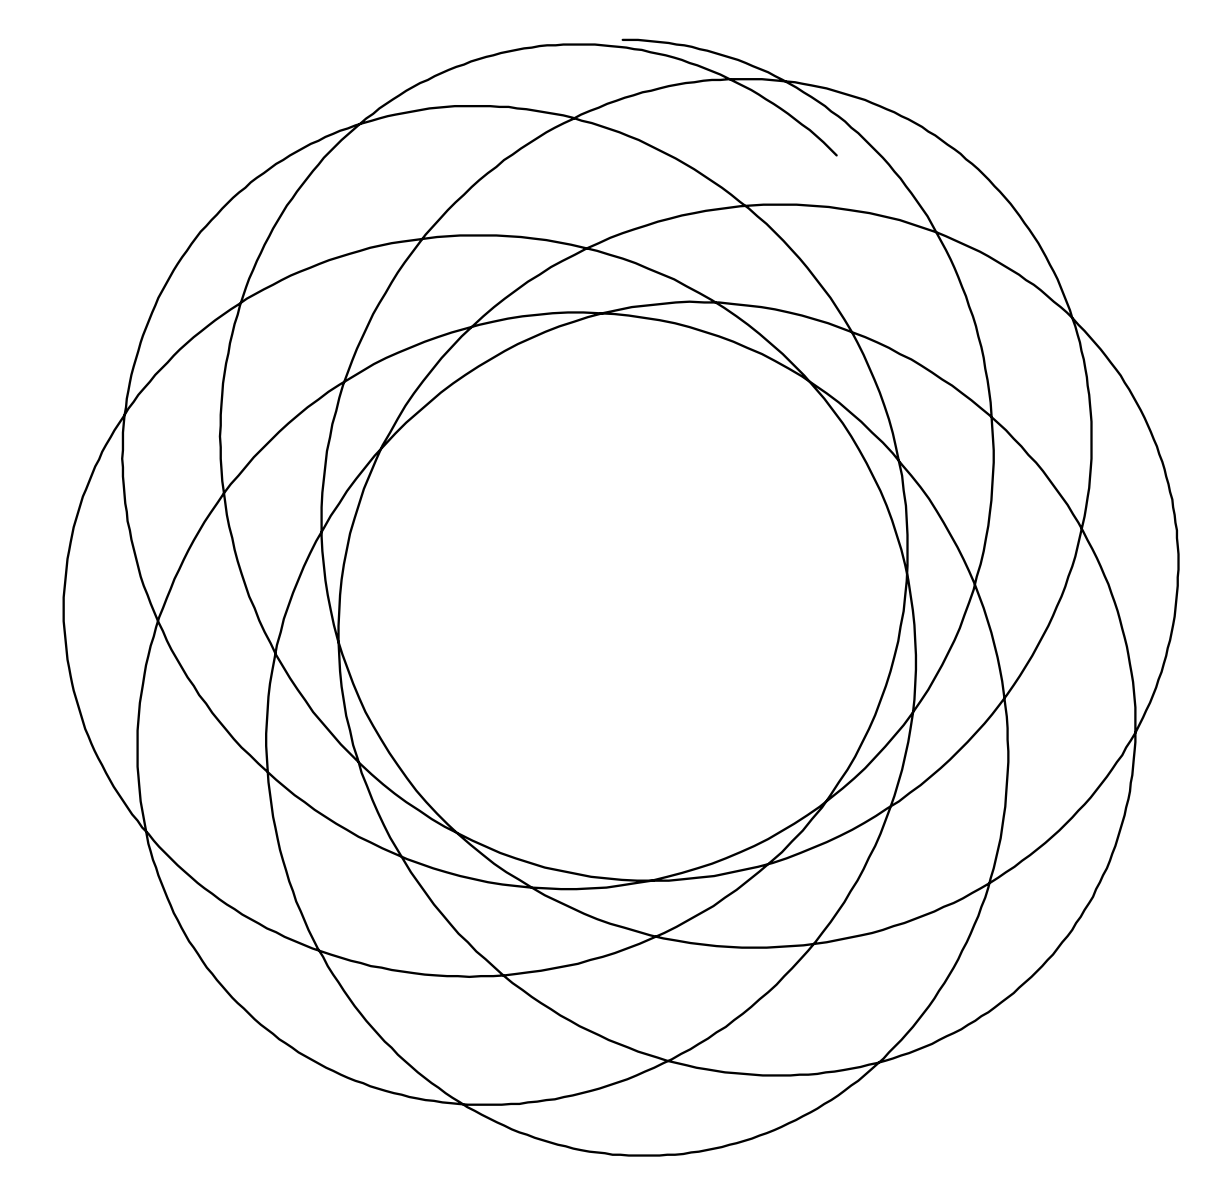
\includegraphics[width=6cm]{figures/rosette.png}}
\end{figure}

{\noindent}\textbf{Spherical harmonic oscillator}

{\noindent}We call a potential of the form

\begin{align*}
    \Phi(r) = \frac{1}{2}\Omega^2r^2 + {\rm constant} ~ [\rm J]
\end{align*}

{\noindent}a spherical harmonic oscillator potential. This potential is generated by a homogeneous sphere of matter. Our modified EOM could be solved analytically in this case, but it is simpler to use Cartesian coordinates A$(x,y)$ defined by $x=r\cos\psi$, $y=r\sin\psi$. In these coordinates, the equations of motion are simply

\begin{align*}
    \ddot{x} = -\Omega^2x; ~~~ \ddot{y} = -\Omega^2y,
\end{align*}

{\noindent}with solutions

\begin{align*}
    x = X\cos(\Omega t+\epsilon_x); ~~~ y = Y\cos(\Omega t+\epsilon_y),
\end{align*}

{\noindent}where $X$, $Y$ , $\epsilon_x$, and $\epsilon_y$ are arbitrary constants. Every orbit is closed since the periods of the oscillations in $x$ and $y$ are identical. The orbits form ellipses centered on the center of attraction. The azimuthal period is $T_\psi=2\pi/\Omega$ because this is the time required for the star to return to its original azimuth. During this time, the particle completes two in-and-out cycles, so the radial period is

\begin{align*}
    T_r = \frac{1}{2}T_\psi = \frac{\pi}{\Omega} ~ [{\rm yr}].
\end{align*}

{\noindent}\textbf{Kepler potential}: When the star is acted on by an inverse-square field $g(r)=−GM/r2$ due to a point mass $M$, the corresponding potential is $\Phi=−GM/r=−GMu$. Motion in this potential is often called \textbf{Kepler motion}. Our modified EOM becomes

\begin{align*}
    \frac{{\rm d}^2u}{{\rm d}\psi^2} + u = \frac{GM}{L^2},
\end{align*}

{\noindent}the general solution of which is

\begin{align*}
    u(\psi) = C\cos(\psi-\psi_0) + \frac{GM}{L^2},
\end{align*}

{\noindent}where $C>0$ and $\psi_0$ are arbitrary constants. Defining the orbit's \textbf{eccentricity} by

\begin{align*}
    e \equiv \frac{CL^2}{GM} ~ [{\rm dimensionless}],
\end{align*}

{\noindent}and its \textbf{semi-major axis} by

\begin{align*}
    q \equiv \frac{L^2}{GM(1-e^2)} ~ [{\rm AU}],
\end{align*}

{\noindent}the general solution may now be written as

\begin{align*}
    r(\psi) = \frac{a(1-e^2)}{1+e\cos(\psi-\psi_0)} ~ [{\rm AU}].
\end{align*}

{\noindent}An orbit for which $e\geq1$ is unbound, since $r\rightarrow\infty$ as $(\psi−\psi_0)\rightarrow\pm\cos^{-1}(−1/e)$. Bound orbits have $e<1$ and along them $r$ is a periodic function of $\psi$ with period $2\pi$, so the star returns to its original radial coordinate after exactly one revolution in $\pi$. Thus bound Kepler orbits are closed, and one may show that they form ellipses with the attracting center at one focus. The pericenter and apocenter distances are

\begin{align*}
    r_1 = a(1-e) ~ [{\rm AU}]; ~~~ r_2 = a(1+e) ~ [{\rm AU}].
\end{align*}

{\noindent}In many applications, $r(\psi)$ for $r$ along a bound Kepler orbit is less convenient than the parameterization

\begin{align*}
    r = a(1-e\cos\eta) ~ [{\rm AU}],
\end{align*}

{\noindent}where the parameter $\eta$ is called the eccentric anomaly to distinguish it from the true anomaly, $\psi-\psi_0$. By equating $r(\psi)$ with this parameterization and using the identity $\cos\theta=(1−\tan^2(\theta/2))/(1+\tan^2(\theta/2))$, it is straightforward to show that the true and eccentric anomalies are related by

\begin{align*}
    \sqrt{1-e}\tan\frac{1}{2}(\psi-\psi_0) = \sqrt{1+e}\tan\frac{1}{2}\eta.
\end{align*}

{\noindent}Taking $t=0$ to occur at pericenter passage, from $L=r^2\dot{\psi}$ we have

\begin{align*}
    t = \int\limits_{\psi_0}^\psi \frac{{\rm d}\psi}{\dot{\psi}} = \int\frac{r^2}{L}{\rm d}\psi = \frac{a^2}{L}\int\limits_0^\eta \frac{{\rm d}\psi}{{\rm d}\eta}(1-e\cos\eta)^2{\rm d}\eta ~ [{\rm yr}].
\end{align*}

{\noindent}Evaluating ${\rm d}\psi/{\rm d}\eta$, integrating, and using trigonometrical identities to simplify the result, we finally obtain

\begin{align*}
    t = \frac{a^2}{L}\sqrt{1-e^2}(\eta-e\sin\eta) = \frac{T_r}{2\pi}(\eta-e\sin\eta) ~ [{\rm yr}],
\end{align*}

{\noindent}where the second equality follows because the bracket on the right increases by $2\pi$ over an orbital period. This is called \textbf{Kepler's equation}, and the quantity $2\pi t/T_r$ is sometimes called the \textbf{mean anomaly}. Hence

\begin{align*}
    T_r = T_\psi = \frac{a^2}{L}\sqrt{1-e^2} = 2\pi\sqrt{\frac{a^3}{GM}} ~ [{\rm yr}].
\end{align*}

{\noindent}The energy per unit mass of a particle on a Kepler orbit is

\begin{align*}
    E = -\frac{GM}{2a} ~ [{\rm J\,kg^{-1}}].
\end{align*}

{\noindent}To unbind the particle, we thus must add the binding energy $−E$.

{\noindent}The study of motion in nearly Kepler potentials is central to the dynamics of planetary systems.

{\noindent}We have shown that a star on a Kepler orbit completes a radial oscillation in the time required for $\psi$ to increase by $\Delta\psi=2\pi$, whereas a star that orbits in a harmonic-oscillator potential has already completed a radial oscillation by the time $\psi$ has increased by $\Delta\psi=\pi$. Since galaxies are more extended than point masses, and less extended than homogeneous spheres, a typical star in a spherical galaxy completes a radial oscillation after its angular coordinate has increased by an amount that lies somewhere in between these two extremes; $\pi<\Delta\psi<2\pi$. Thus, we expect a star to oscillate from its apocenter through its pericenter and back in a shorter time than is required for one complete azimuthal cycle about the galactic center.

{\noindent}It is sometimes useful to consider that an orbit in a non-Kepler force field forms an approximate ellipse, though one that precesses by $\psi_p=\Delta\psi−2\pi$ in the time needed for one radial oscillation. For the orbit shown in Figure \ref{fig:rosette}, and most galactic orbits, this precession is in the sense opposite to the rotation of the star itself. The angular velocity $\Omega_p$ of the rotating frame in which the ellipse appears closed is

\begin{align*}
    \Omega_p = \frac{\psi_p}{T_r} = \frac{\Delta\psi-2\pi}{T_r} ~ [{\rm rad\,yr^{-1}}].
\end{align*}

{\noindent}Hence we say that $\Omega_p$ is the \textbf{precession rate} of the ellipse. The concept of closed orbits in a rotating frame of reference is crucial to the theory of spiral structure -- see Figure \ref{fig:closedorbits}.

\begin{figure}[t]
    \centering
    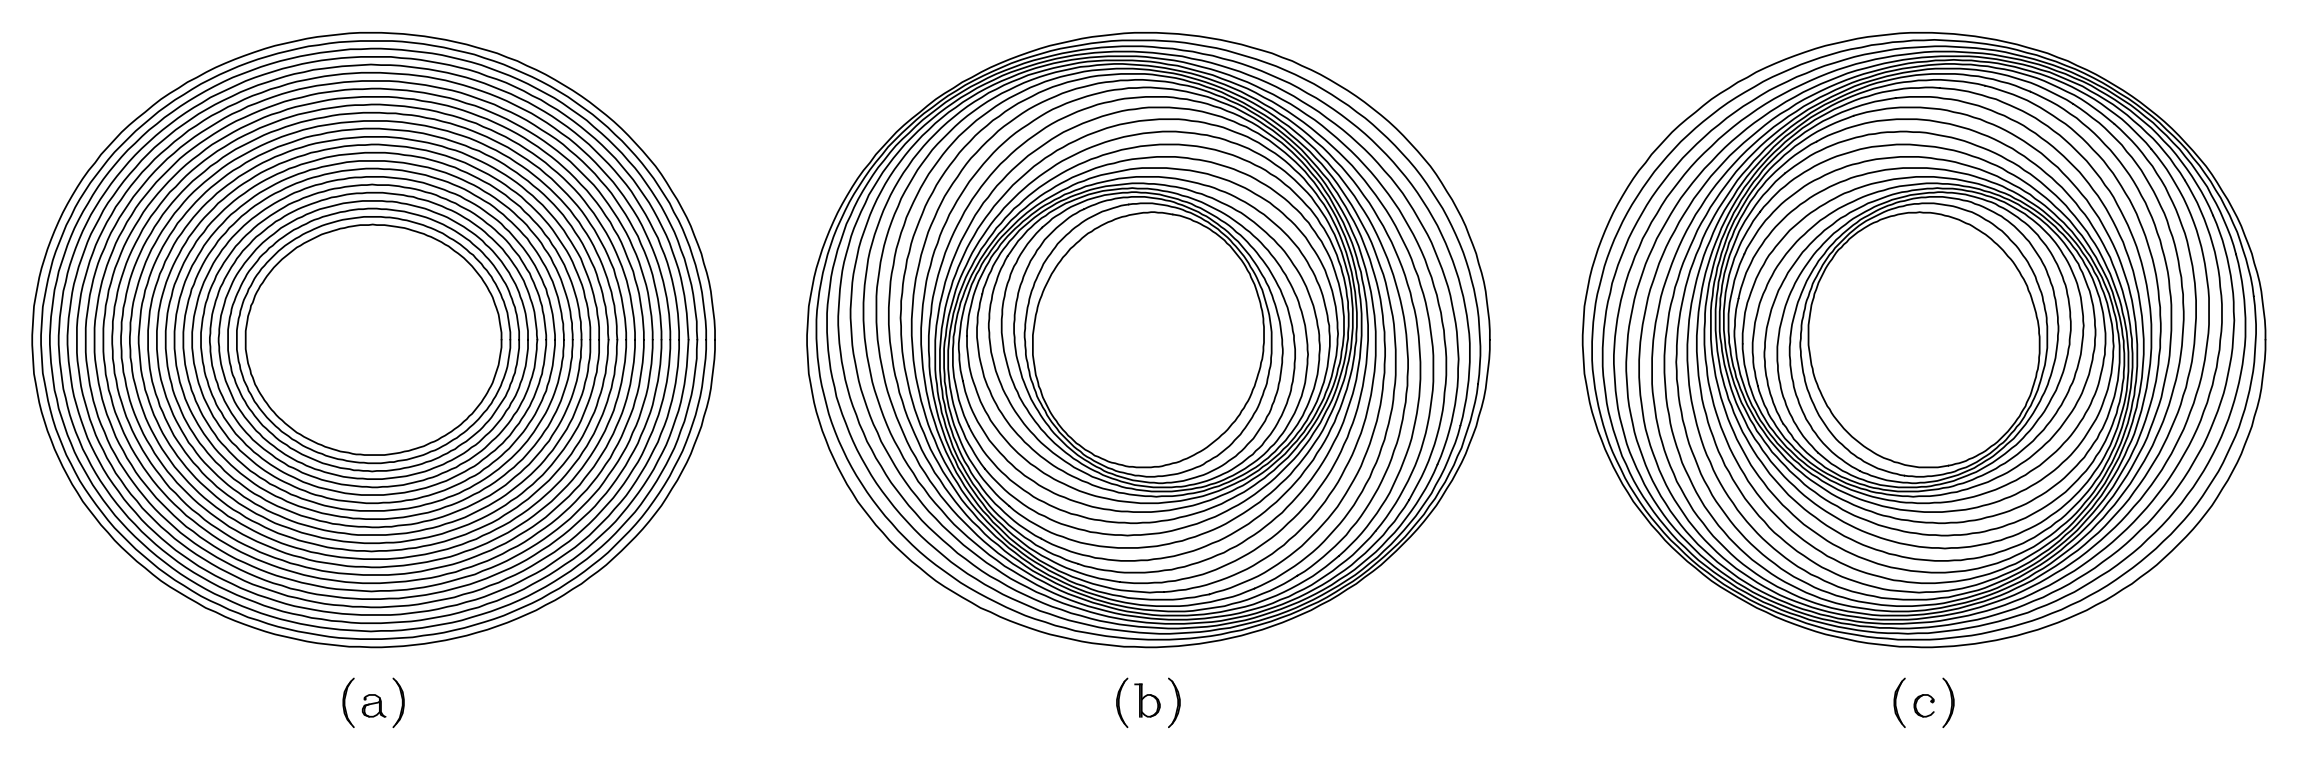
\includegraphics[width=16cm]{figures/ClosedOrbits.png}
    \caption{\footnotesize{Arrangement of closed orbits in a galaxy to create bars and spiral patterns. Figure taken from Binney \& Tremaine (2011).}}
    \label{fig:closedorbits}
\end{figure}

{\noindent}\textbf{Isochrone potential}

{\noindent}The harmonic oscillator and Kepler potentials are both generated by mass distributions that are qualitatively different from the mass distributions of galaxies. The only known potential that could be generated by a realistic stellar system for which all orbits are analytic is the isochrone potential:

\begin{align*}
    \Phi(r) = - \frac{GM}{b + \sqrt{b^2+r^2}} ~ [{\rm J}].
\end{align*}

{\noindent}\textbf{2. Orbits in axisymmetric potentials}

{\noindent}Few galaxies are even approximately spherical, but many approximate figures of revolution. Thus we begin to explore the types of orbits that are possible in many real galaxies. We shall usually employ a cylindrical coordinate system $(R,\phi,z)$ with origin at the galactic center, and shall align the $z$ axis with the galaxy's symmetry axis.

{\noindent}Stars whose motions are confined to the equatorial plane of an axisymmetric galaxy have no way of perceiving that the potential in which they move is not spherically symmetric. Therefore their orbits will be identical with in symmetric potentials; the radial coordinate $R$ of a star on such an orbit oscillates between fixed extrema as the star revolves around the center, and the orbit again forms a rosette figure.

{\noindent}\textbf{Motion in the meridional plane}

{\noindent}The situation is much more complex and interesting for stars whose motions carry them out of the equatorial plane of the system. The study of such general orbits in axisymmetric galaxies can be reduced to a two-dimensional problem by exploiting the conservation of the $z$-component of angular momentum of any star. Let the potential, which we assume to be symmetric about the plane $z=0$, be $\Phi(R,z)$. Then the motion is governed by the Lagrangian

\begin{align*}
    \mathcal{L} = \frac{1}{2}[\dot{R}^2+(R\dot{\phi})^2+\dot{z}^2] - \Phi(R,z) ~ [{\rm J}].
\end{align*}

{\noindent}The momenta are

\begin{align*}
    p_R=\dot{R}; ~~~ p_\phi=R^2\dot{\phi}; ~~~ p_z=\dot{z},
\end{align*}

{\noindent}so the Hamiltonian is

\begin{align*}
    H = \frac{1}{2}\left(P_R^2+\frac{p_\phi^2}{R^2}+p_z^2\right) + \Phi(R,z) ~ [{\rm J}].
\end{align*}

{\noindent}From Hamilton's equations we find that the equations of motion are

\begin{align*}
    \dot{p_r} &= \ddot{R} = \frac{p_\phi^2}{R^3} - \frac{\partial\Phi}{\partial R} \\
    \dot{p_\phi} &= \frac{{\rm d}}{{\rm d}t}(R^2\dot{\phi}) = 0 \\
    \dot{p_z} &= \ddot{z} = - \frac{\partial\Phi}{\partial z}.
\end{align*}

{\noindent}The second of these EOMs expresses conservation of the component of angular momentum about the $z$ axis, $p_\phi=L_z$ (a constant), while the first and second describe the coupled oscillations of the star in the $R$ and $z$-directions.

{\noindent}After replacing $p_\phi$ in the first of these EOMs by its numerical value $L_z$, the first and last of these EOMs can be written

\begin{align*}
    \ddot{R}=-\frac{\partial\Phi_{\rm eff}}{\partial R}; ~~~ \ddot{z}=-\frac{\partial\Phi_{\rm eff}}{\partial z},
\end{align*}

{\noindent}where

\begin{align*}
    \Phi_{\rm eff} \equiv \Phi(R,z) + \frac{L_z^2}{2R^2}
\end{align*}

{\noindent}is called the \textbf{effective potential}. Thus the three-dimensional motion of a star in an axisymmetric potential $\Phi(R,z)$ can be reduced to the two-dimensional motion of the star in the $(R,z)$ plane (the meridional plane) under the Hamiltonian

\begin{align*}
    H_{\rm eff} = \frac{1}{2}(p_R^2+p_z^2) + \Phi_{\rm eff}(R,z) ~ [{\rm J}]. 
\end{align*}

{\noindent}Notice that $H_{\rm eff}$ differs from the full Hamiltonian only in the substitution of the constant $L_z$ for the azimuthal momentum $p_\phi$. Consequently, the numerical value of $H_{\rm eff}$ is simply the orbit's total energy $E$. The difference $E−\Phi_{\rm eff}$ is the kinetic energy of motion in the $(R,z)$ plane, equal to $(p_R^2+p_z^2)/2$. Since kinetic energy is non-negative, the orbit is restricted to the area in the meridional plane satisfying the inequality $E\geq\Phi_{\rm eff}$. The curve bounding this area is called the zero-velocity curve, since the orbit can only reach this curve if its velocity in the $(R,z)$ plane is instantaneously zero.

\begin{figure}[t]
    \centering
    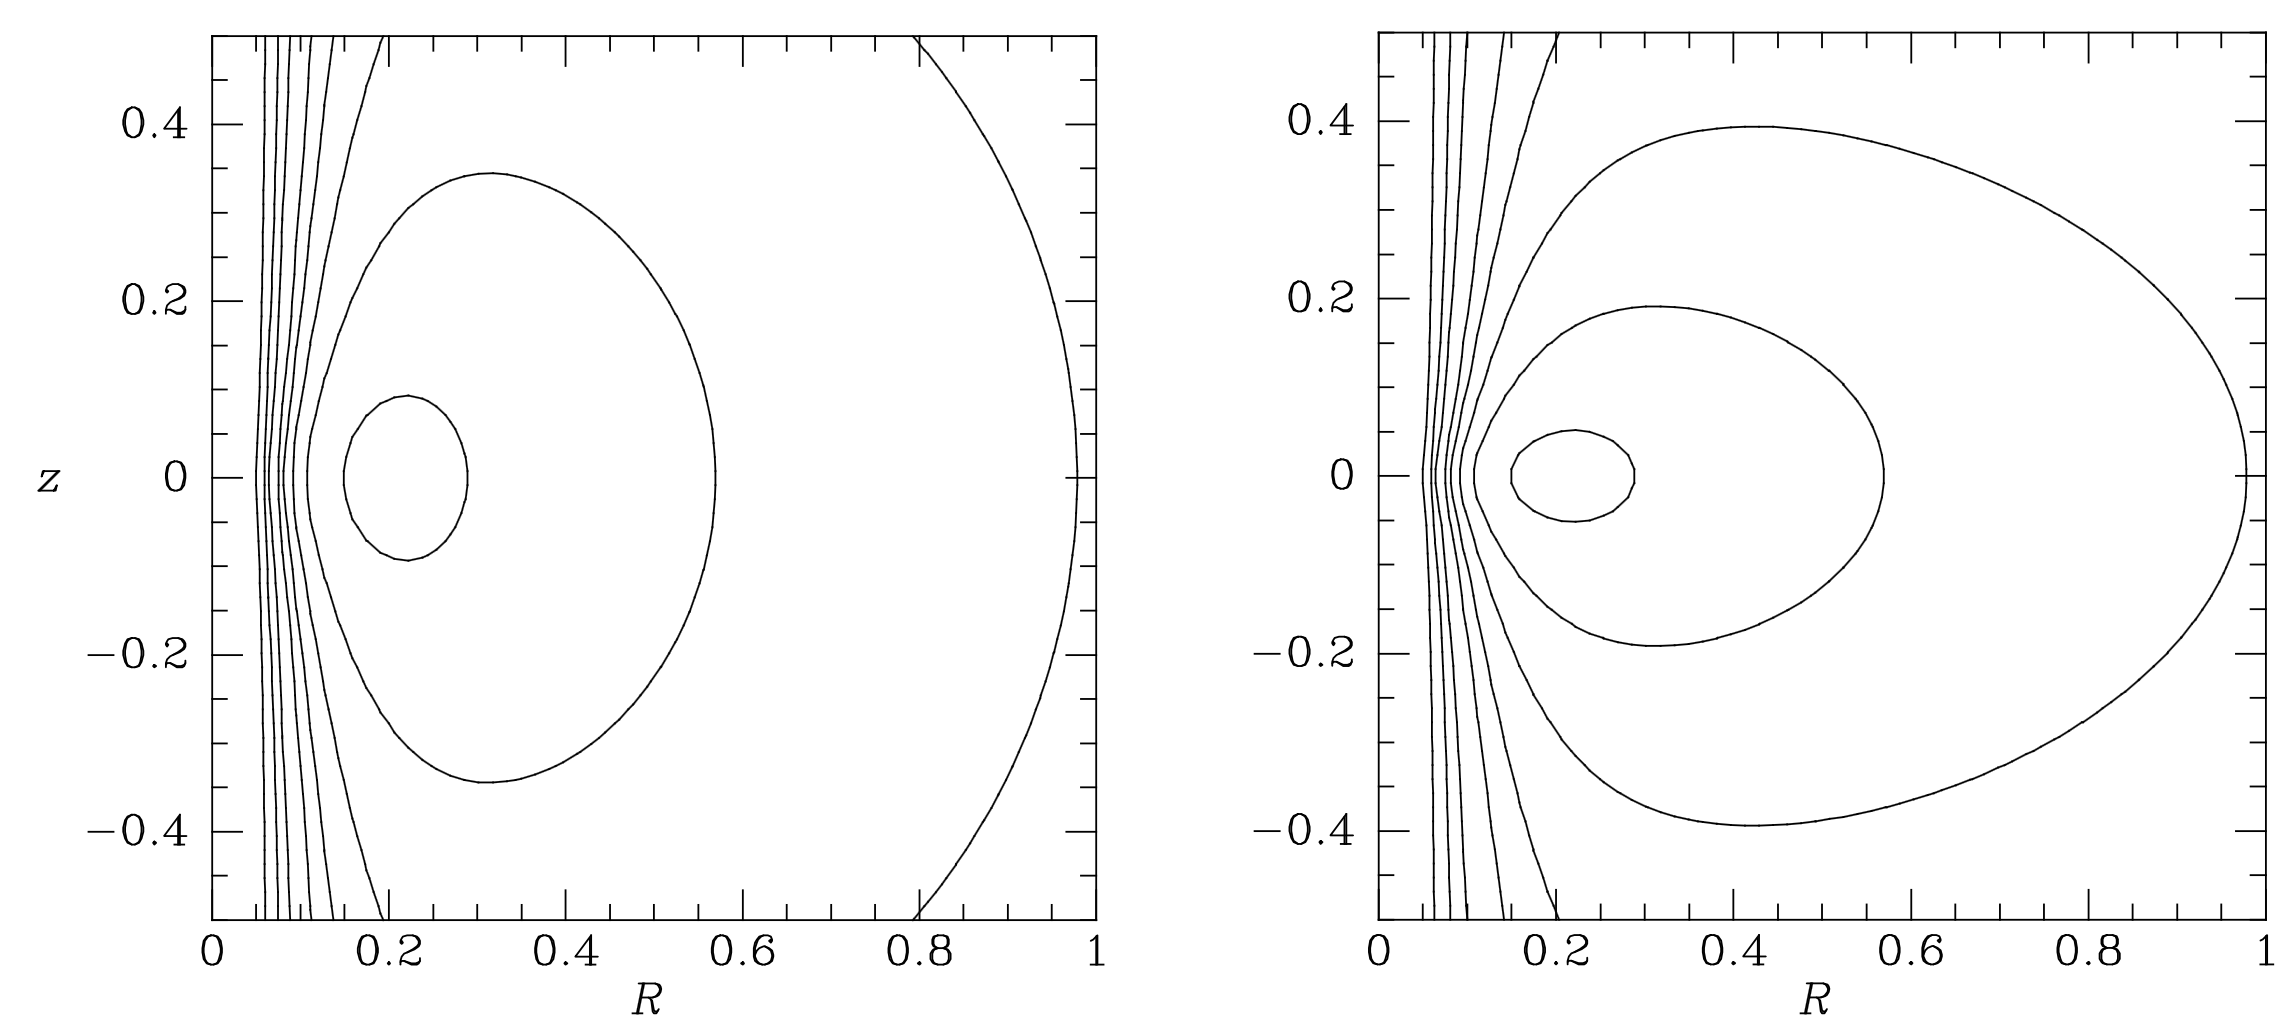
\includegraphics[width=16cm]{figures/EffPot.png}
    \caption{\footnotesize{Two orbits in an effective potential $\Phi_{\rm eff}$ with $q=0.9$. Both orbits are at energy $E=−0.8$ and angular momentum $L_z=0.2$, and we assume $v_0=1$. Figure taken from Binney \& Tremaine (2011).}}
    \label{fig:effpot}
\end{figure}

{\noindent}Figure \ref{fig:effpot} shows contour plots of the effective potential

\begin{align*}
    \Phi_{\rm eff} = \frac{1}{2}v_0^2\ln \left(R^2 + \frac{z^2}{q^2}\right) + \frac{L_z^2}{2R^2} ~ [{\rm J}],
\end{align*}

{\noindent}for $v_0=1$, $L_z=0.2$ and axial ratios $q=0.9$ and $0.5$. This resembles the effective potential experienced by a star in an oblate spheroidal galaxy that has a constant circular speed $v_0$. Notice that $\Phi_{\rm eff}$ rises very steeply near the $z$ axis, as if the axis of symmetry were protected by a \textbf{centrifugal barrier}.

{\noindent}The minimum in $\Phi_{\rm eff}$ has a simple physical significance. The minimum occurs where

\begin{align*}
    \frac{\partial\Phi_{\rm eff}}{\partial R} = \frac{\partial\Phi}{\partial R} - \frac{L_z^2}{R^3} = 0; ~~~ \frac{\partial\Phi_{\rm eff}}{\partial z} = 0.
\end{align*}

{\noindent}The second of these conditions is satisfied anywhere in the equatorial plane $z=0$ on account of the assumed symmetry of $\Phi$ about this place, and the first is satisfied at the guiding-center radius $R_g$ where

\begin{align*}
    \left(\frac{\partial\Phi}{\partial R}\right)_{(R_g,0)} = \frac{L_z^2}{R_g^3} = R_g\dot{\phi}^2.
\end{align*}

{\noindent}This is simply the condition for a circular orbit with angular speed $\dot{\phi}$. Thus the minimum of $\Phi_{\rm eff}$ occurs at the radius at which a circular orbit has angular momentum $L_z$, and the value of $\Phi_{\rm eff}$ at the minimum is the energy of this circular orbit.

\begin{figure}[t]
    \centering
    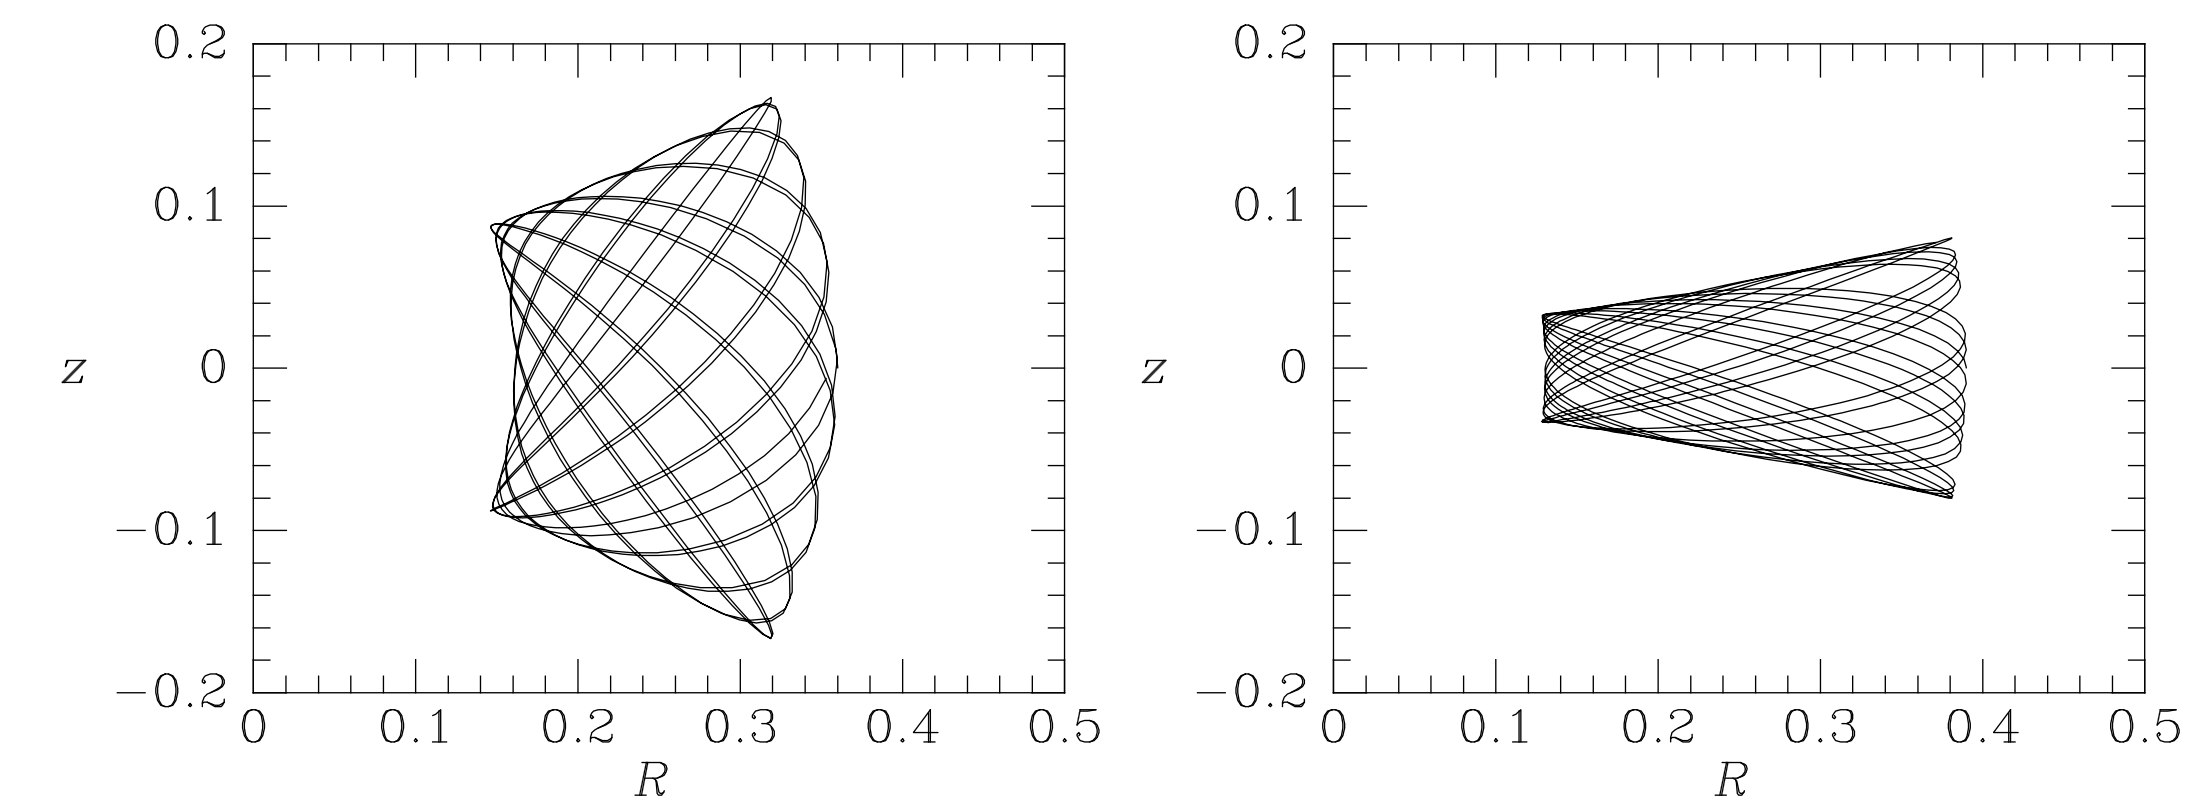
\includegraphics[width=16cm]{figures/AxisymmOrbits.png}
    \caption{\footnotesize{Two orbits in the effective potential $\Phi_{\rm eff}$ with $q=0.9$. Both orbits are at energy $E=−0.8$ and angular momentum $L_z=0.2$, and we assume $v_0=1$. Figure taken from Binney \& Tremaine (2011).}}
    \label{fig:axisymmorbits}
\end{figure}

{\noindent}Unless the gravitational potential $\Phi$ is of some special form, the EOMs for $\ddot{R}$ and $\ddot{z}$ cannot be solved analytically. However, we may follow the evolution of $R(t)$ and $z(t)$ by integrating them numerically, starting from a variety of initial conditions. Figure \ref{fig:axisymmorbits} shows the result of two such integrations for the effective potential $\Phi_{\rm eff}$ with $q=0.9$. The orbits shown are of stars of the same energy and angular momentum, yet they look quite different in real space, and hence the stars on these orbits must move through different regions of phase space. Is this because the equations of motion admit a third isolating integral $I(R,z,p_R,p_z)$ in addition to $E$ and $L_z$?

{\noindent}\textbf{Surfaces of section}

{\noindent}The phase space associated with the motion we are considering has four dimensions, $R$, $z$, $p_R$, and $p_z$, and the four-dimensional motion of the phase-space point of an individual star is too complicated to visualize. Nonetheless, we can determine whether orbits in the $(R,z)$ plane admit an additional isolating integral by use of a simple graphical device. Since the Hamiltonian $H_{\rm eff}(R,z,p_R,p_z)$ is constant, we could plot the motion of the representative point in a three-dimensional reduced phase space, say $(R,z,p_R)$, and then $p_z$ would be determined (to within a sign) by the known value $E$ of $H_{\rm eff}$. However, even three-dimensional spaces are difficult to draw, so we simply show the points where the star crosses some plane in the reduced phase space, say the plane $z=0$; these points are called \textbf{consequents}. To remove the sign ambiguity in $p_z$, we plot the $(R,p_R)$ coordinates only when $p_z>0$. In other words, we plot the values of $R$ and $p_R$ every time the star crosses the equator going upward. Such plots were first used by Poincar\'e and are called \textbf{surfaces of section}. The key feature of the surface of section is that, even though it is only two-dimensional, no two distinct orbits at the same energy can occupy the same point. Also, any orbit is restricted to an area in the surface of section defined by the constraint $Heff\geq(\dot{R}^2+\Phi_{\rm eff})/2$; the curve bounding this area is often called the zero-velocity curve of the surface of section, since it can only be reached by an orbit with $p_z=0$.

\begin{figure}[t]
    \floatbox[{\capbeside\thisfloatsetup{capbesideposition={right,top},capbesidewidth=4cm}}]{figure}[\FBwidth]
    {\caption{\footnotesize{Points generated by the orbit of the left panel of Figure \ref{fig:axisymmorbits} in the $(R,p_R)$ surface of section. If the total angular momentum $L$ of the orbit were conserved, the points would fall on the dashed curve. The full curve is the zero-velocity curve at the energy of this orbit. The $\times$ marks the consequent of the shell orbit. Figure taken from Binney \& Tremaine (2011).}}
    \label{fig:surfacesection}}
    {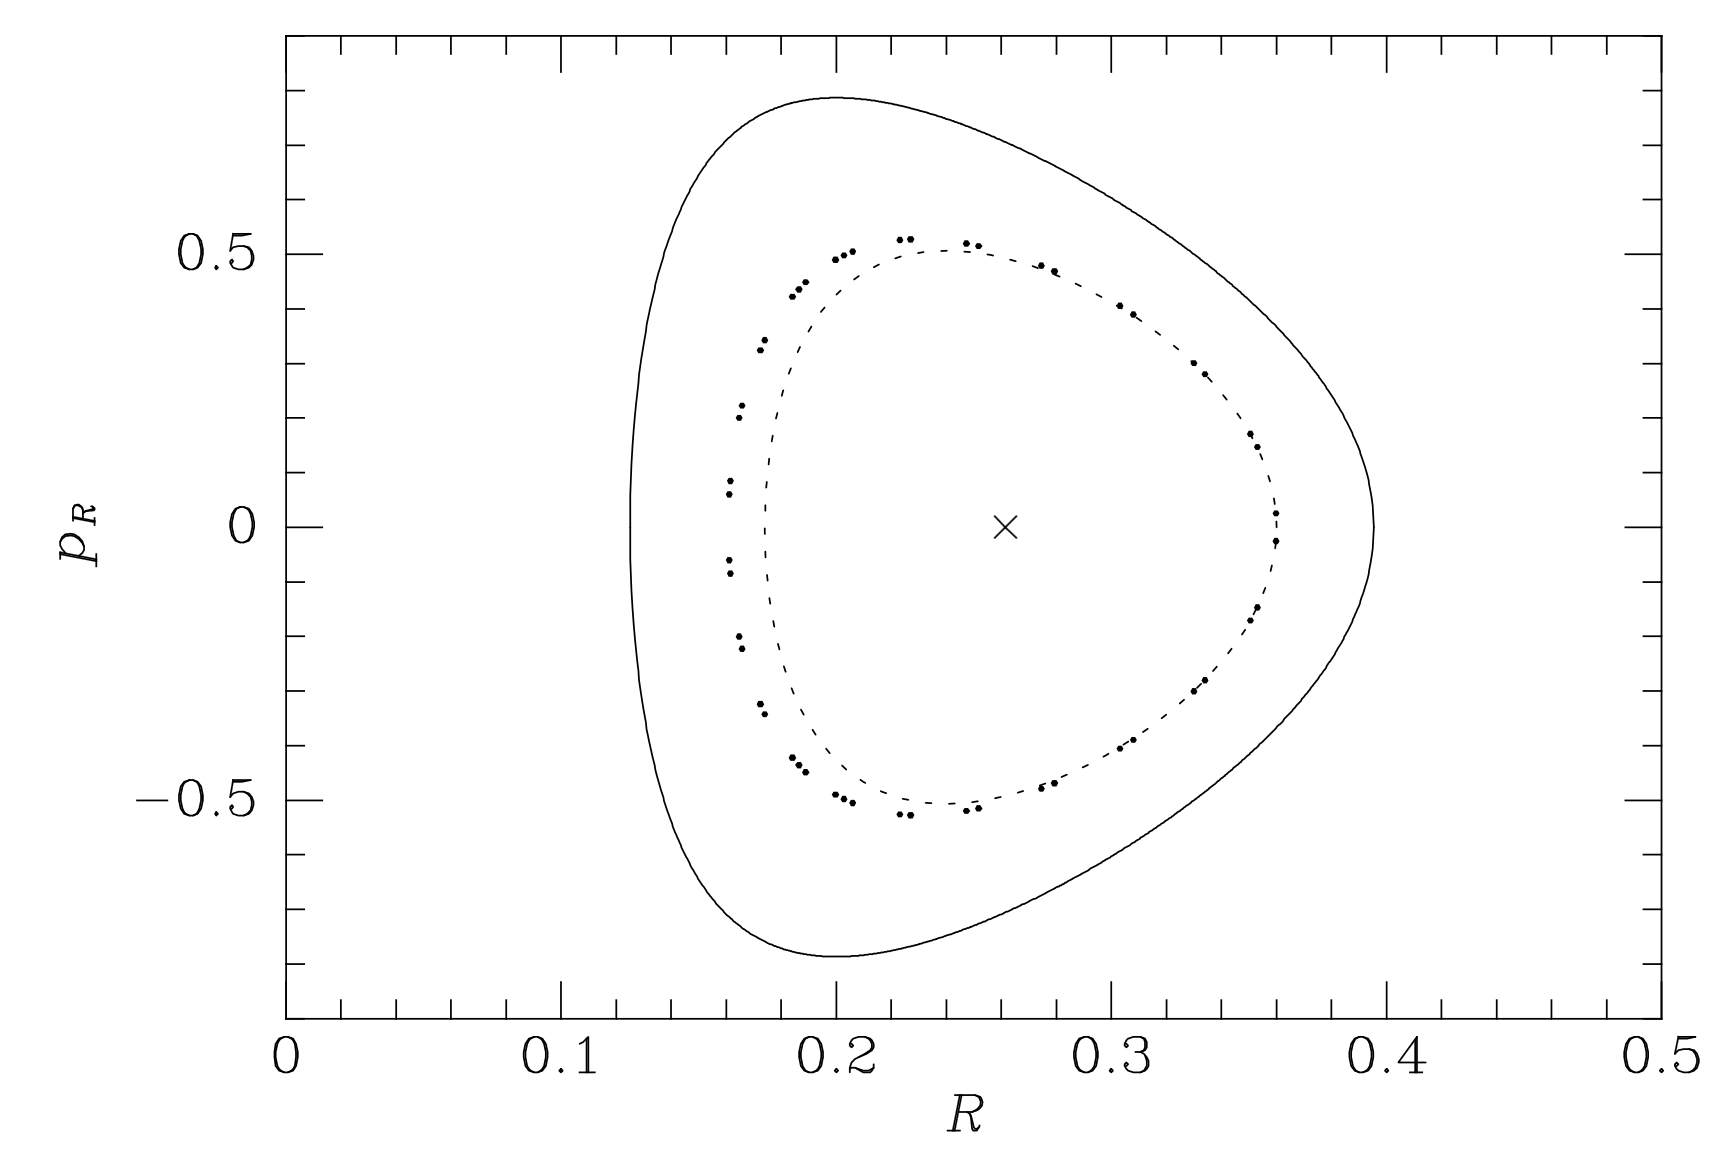
\includegraphics[width=10cm]{figures/SurfaceSection.png}}
\end{figure}

\begin{figure}[t]
    \floatbox[{\capbeside\thisfloatsetup{capbesideposition={left,top},capbesidewidth=4cm}}]{figure}[\FBwidth]
    {\caption{\footnotesize{The total angular momentum is almost constant along the orbit shown in the left panel of Figure \ref{fig:axisymmorbits}. For clarity $L(t)$ is plotted only at the beginning and end of a long integration. Figure taken from Binney \& Tremaine (2011).}}
    \label{fig:lvst}}
    {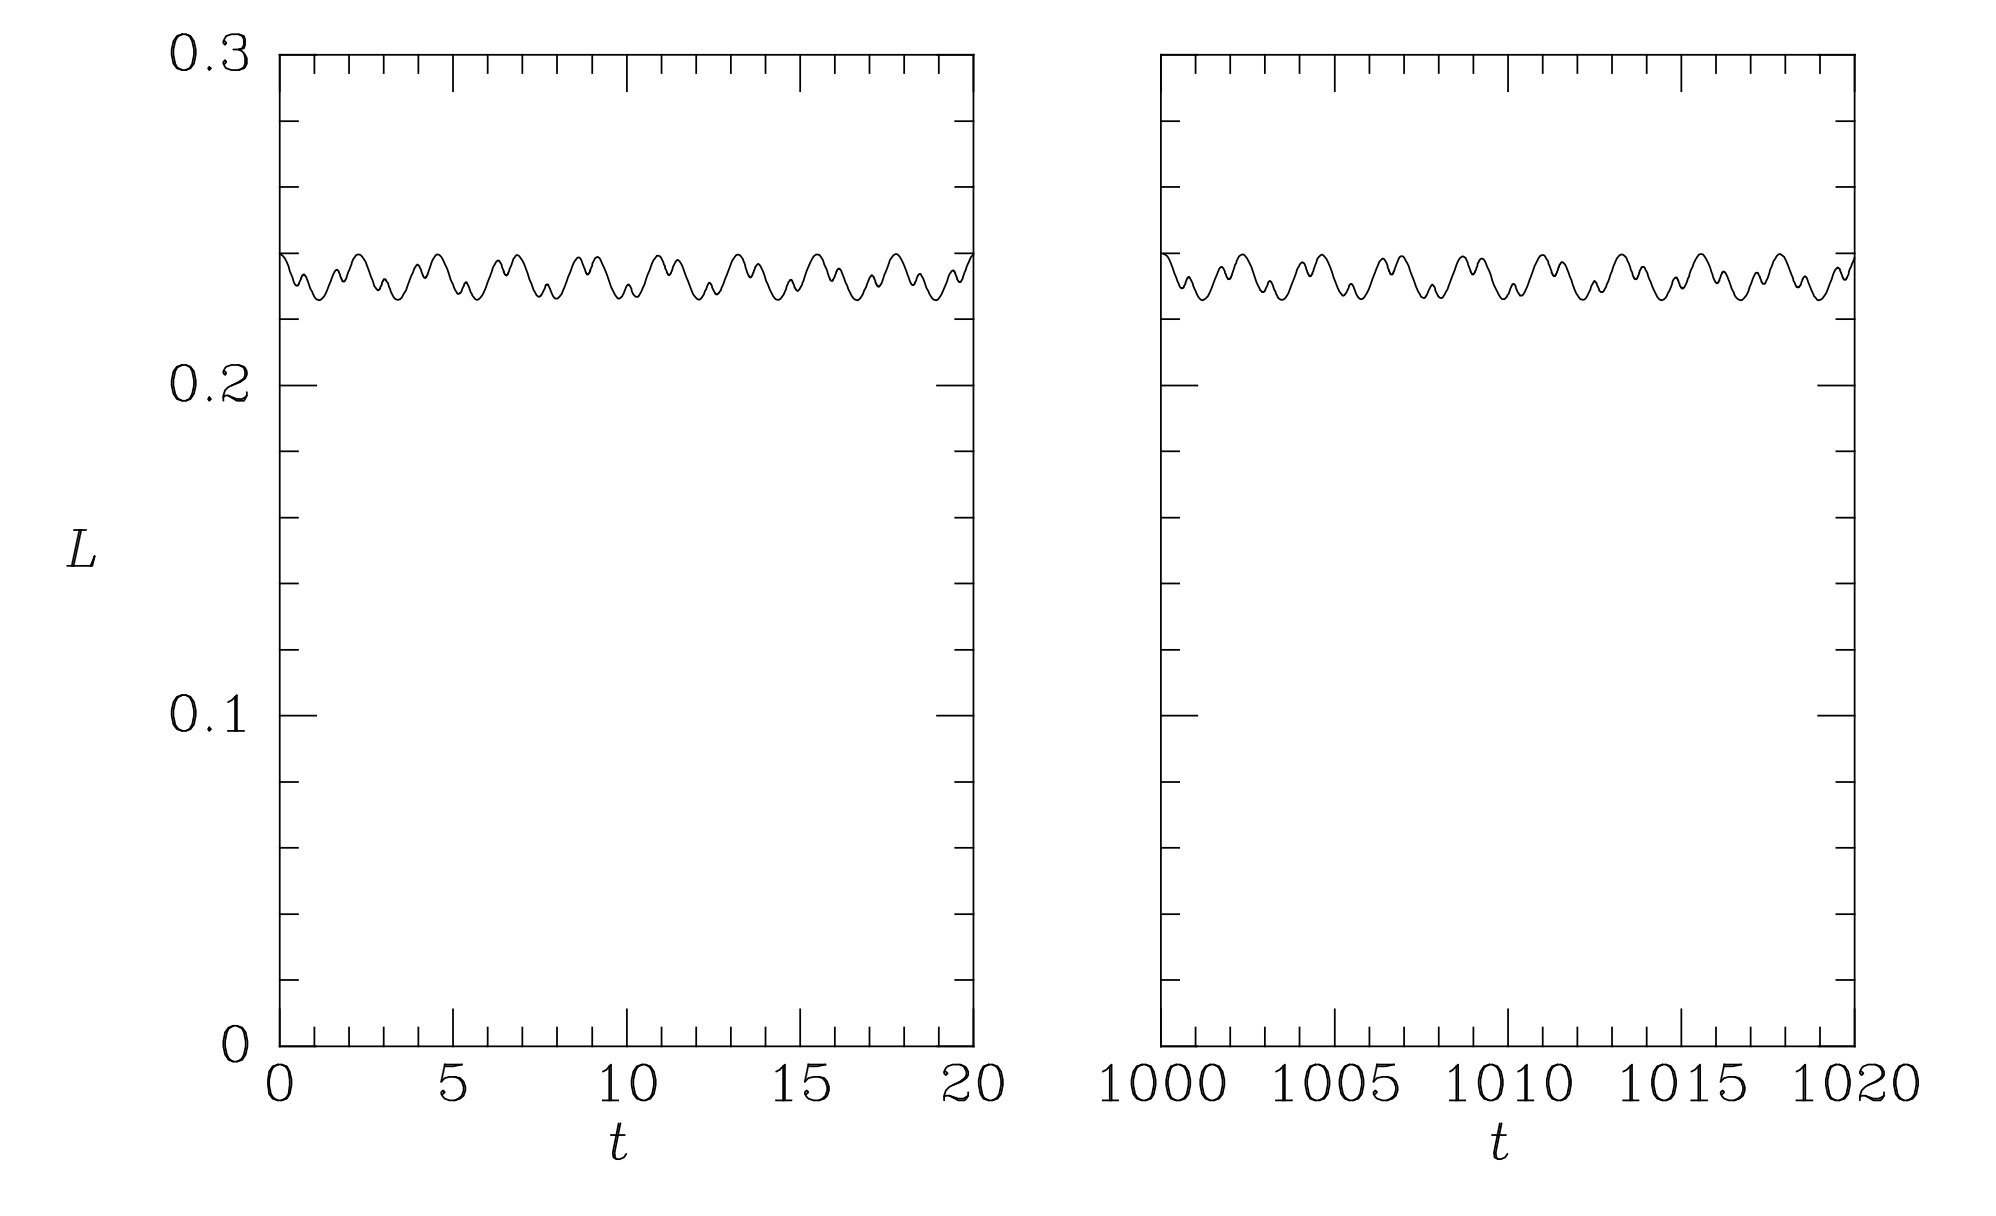
\includegraphics[width=10cm]{figures/Lvst.png}}
\end{figure}

{\noindent}Figure \ref{fig:surfacesection} shows the $(R,p_R)$ surface of section at the energy of the orbits of Figure \ref{fig:axisymmorbits}: the full curve is the zero-velocity curve, while the dots show the consequents generated by the orbit in the left panel of Figure \ref{fig:axisymmorbits}. The cross near the center of the surface of section, at $(R=0.26,p_R=0)$, is the single consequent of the shell orbit, in which the trajectory of the star is restricted to a two-dimensional surface. The shell orbit is the limit of orbits such as those shown in Figure \ref{fig:axisymmorbits} in which the distance between the inner and outer boundaries of the orbit shrinks to zero.

{\noindent}In Figure \ref{fig:surfacesection} the consequents of the orbit of the left panel of Figure \ref{fig:axisymmorbits} appear to lie on a smooth curve, called the invariant curve of the orbit. The existence of the invariant curve implies that some isolating integral $I$ is respected by this orbit. The curve arises because the equation $I={\rm constant}$ restricts motion in the two-dimensional surface of section to a one-dimensional curve (or perhaps to a finite number of discrete points in exceptional cases). It is often found that for realistic galactic potentials, orbits do admit an integral of this type. Since $I$ is in addition to the two classical integrals $H$ and $p_\phi$, it is called the \textbf{third integral}. In general there is no analytic expression for $I$ as a function of the phase-space variables, so it is called a \textbf{non-classical integral}.

{\noindent}We may form an intuitive picture of the nature of the third integral by considering two special cases. If the potential $\Phi$ is spherical, we know that the total angular momentum $|\vec{L}|$ is an integral. This suggests that for a nearly spherical potential (this one has axis ratio $q=0.9$) the third integral may be approximated by $|\vec{L}|$. The dashed curve in Figure \ref{fig:surfacesection} shows the curve on which the points generated by the orbit of the left panel of Figure \ref{fig:axisymmorbits} would lie if the third integral were $|\vec{L}|$, and Figure \ref{fig:lvst} shows the actual time evolution of $|\vec{L}|$ along that orbit -- notice that although $|\vec{L}|$ oscillates rapidly, its mean value does not change even over hundreds of orbital times. From these two figures we see that $|\vec{L}|$ is an approximately conserved quantity, even for orbits in potentials that are significantly flattened. We may think of these orbits as approximately planar and with more or less fixed peri- and apocenter radii. The approximate orbital planes have a fixed inclination to the $z$ axis but precess about this axis, at a rate that gradually tends to zero as the potential becomes more and more nearly spherical.

{\noindent}The second special case is when the potential is separable in $R$ and $z$:

\begin{align*}
    \Phi(R,z)=\Phi_R(R)+\Phi_z(z) ~ [{\rm J}].
\end{align*}

{\noindent}Then the third integral can be taken to be the energy of vertical motion

\begin{align*}
    H_z = \frac{1}{2}p_z^2 + \Phi_z(z) ~ [{\rm J}].
\end{align*}

{\noindent}Along nearly circular orbits in a thin disk, the potential is approximately separable, so this equation provides a useful expression for the third integral.

{\noindent}\textbf{Elliptical galaxies}

{\noindent}Elliptical galaxies nearly always have cusps in their central density profiles in which $\rho\sim r^{-\alpha}$ with $0.3\lesssim\alpha\lesssim2$. Black holes with masses $\sim0.2\%$ of the mass of the visible galaxy are believed to reside at the centers of these cusps. Further out the mass distributions of many elliptical galaxies are thought to be triaxial. These features make the orbital dynamics of elliptical dynamics especially rich.

{\noindent}A useful basic model of the orbital dynamics of a triaxial elliptical galaxy is provided by extensions to three dimensions of the two-dimensional St\"{a}ckel potentials. The simplest three-dimensional system that generates a St\"{a}ckel potential through Poisson's equation is the \textbf{perfect ellipsoid}, in which the density is given by

\begin{align*}
    \rho(x) = \frac{\rho_0}{(1+m^2)^2}
\end{align*}

{\noindent}where

\begin{align*}
    m^2 \equiv \frac{x^2+(y/q_1)^2+(z/q_2)^2}{a_0^2}.
\end{align*}

{\noindent}In this formula $q_1$ and $q_2$ are the axis ratios of the ellipsoidal surfaces of constant density, and $a_0$ is a scale length. At radii significantly smaller than $a_0$, the density is approximately constant, while at $r\gg a_0$ the density falls off $\propto r^{4-}$. Since these asymptotic forms differ from those characteristic of elliptical galaxies, we have to expect the orbital structures of real galaxies to differ in detail from that of the perfect ellipsoid, but nevertheless the model exhibits much of the orbital structure seen in real elliptical galaxies.

\begin{figure}[t!]
    \centering
    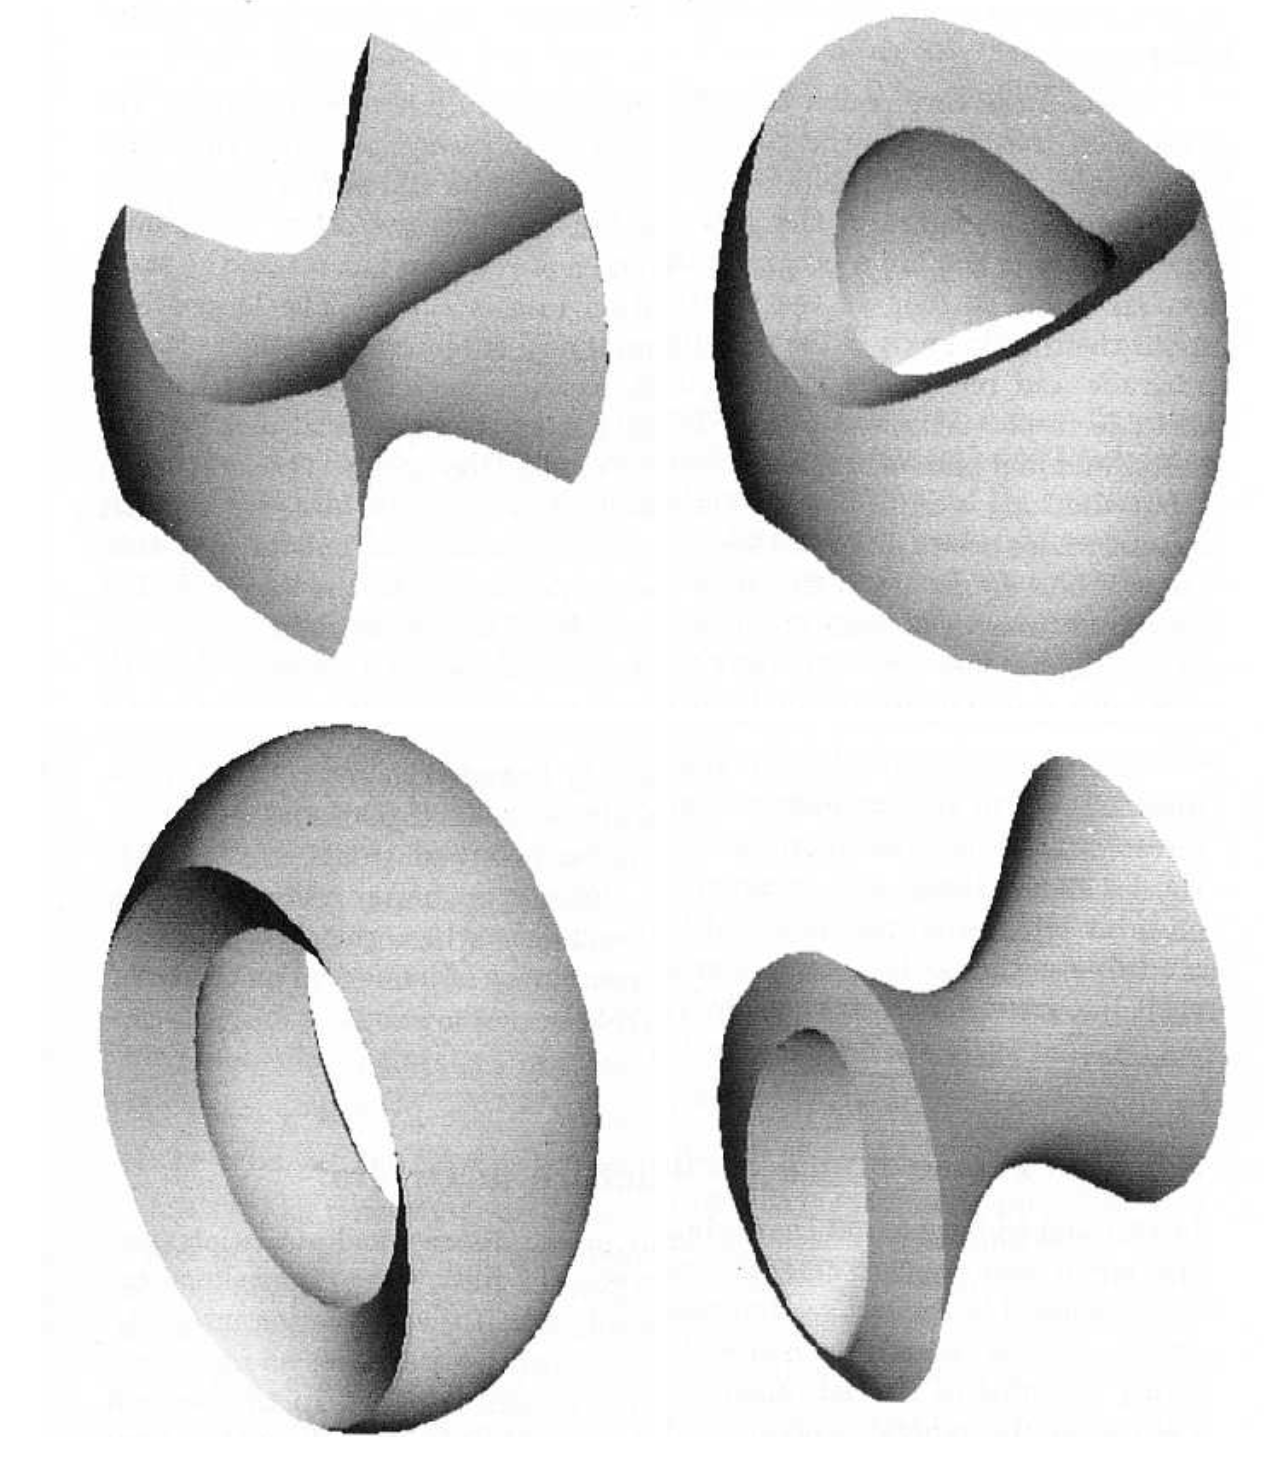
\includegraphics[width=8cm]{figures/TriaxialOrbits.png}
    \caption{\footnotesize{Orbits in a non-rotating triaxial potential. Clockwise from top left: (a) box orbit; (b) short-axis tube orbit; (c) inner long-axis tube orbit; (d) outer long-axis tube orbit. From Statler (1987), by permission of the AAS. Figure taken from Binney \& Tremaine (2011).}}
    \label{fig:triaxialorbits}
\end{figure}

{\noindent}By an analysis similar to that used to explore the potential of a planar bar, one can show that the perfect ellipsoid supports four types of orbits. Figure 3.46 depicts an orbit of each type. At top left we have a box orbit. The key feature of a box orbit is that it touches the isopotential surface for its energy at its eight corners. Consequently, the star comes to rest for an instant at these points; a box orbit is conveniently generated numerically by releasing a star from rest on the equipotential surface. The potential's longest axis emerges from the orbit’s convex face. The other three orbits are all tube orbits: stars on these orbits circulate in a fixed sense around the hole through the orbit's center, and are never at rest. The most important tube orbits are the short-axis loops shown at top right, which circulate around the potential's shortest axis. These orbits are mildly distorted versions of the orbits that dominate the phase space of a flattened axisymmetric potential. The tube orbits at the bottom of Figure 3.46 are called outer (left) and inner long-axis tube orbits, and circulate around the longest axis of the potential. Tube orbits around the intermediate axis are unstable. All these orbits can be quantified by a single system of angle-action coordinates $(J_\lambda,J_\mu,J_\nu)$ that are generalizations of the angle-action coordinates for spherical potentials $(J_r,J_\theta,J_\phi)$.

\begin{itemize}
    \item If we perturb a star in the disk in the z-direction, what happens?
    \item If we perturb a star in the disk in the radial-direction, what happens?
    \item What are the observed quantities in each scenario?
    \item How many integrals of motion are there in the disk?
    \item What symmetry leads to energy conservation?
\end{itemize}


% --------------------------------------------------------------
%               3. 
% --------------------------------------------------------------

\newpage
\subsection{Question 3}

Every now and then a supernova explosion occurs within $3\,\mathrm{pc}$ of the Earth. Estimate how long one typically has to wait for this to happen. Why are newborn stars likely to experience this even when they are much younger than the waiting time you have just estimated?

\subsubsection{Short answer}

Answer.

\subsubsection{Additional context}

Additional context.

% --------------------------------------------------------------
%               4. 
% --------------------------------------------------------------

\newpage
\subsection{Question 4}

Galactic stars are described as a collision-less system. Why? (Don’t forget the influence of gravity.)

\subsubsection{Short answer}

Answer.

\subsubsection{Additional context}

Additional context.

\subsubsection{Follow-up Questions}

\begin{itemize}
    \item What happens when stars collide?
    \item Why choose a cross-section that's larger than the star's radius?
    \item What impact parameter do we need for the stars to end up physically touching (calculate it)?
\end{itemize}

% --------------------------------------------------------------
%               5. 
% --------------------------------------------------------------

\newpage
\subsection{Question 5}

Given that only a tiny fraction of the mass of the interstellar medium consists of dust, why is dust important to the chemistry of the medium and to the formation of stars?

\subsubsection{Short answer}

Dust is understood to play many critical roles in galactic evolution. By sequestering selected elements in the solid grains, and by catalyzing formation of the H$_2$ molecule, dust grains are central to the chemistry of interstellar gas. Photoelectrons from dust grains can dominate the heating of gas in regions where UV starlight is present, and in dense regions the infrared emission from dust can be an important cooling mechanism. Last, dust grains can be important in interstellar gas dynamics, communicating radiation pressure from starlight to the gas, and coupling the magnetic field to the gas in regions of low fractional ionization.

\subsubsection{Additional context}

Our strongest constraints on interstellar dust come from observations of its interaction with electromagnetic radiation:

\begin{itemize}
    \item Wavelength-dependent attenuation (``extinction'') of starlight by absorption and scattering, now observable at wavelengths as long as $20\,\mu{\rm m}$ (``mid-infrared''), and as short as $0.1\,\mu{\rm m}$ (``vacuum ultraviolet''). The extinction includes a number of spectral features that provide clues to grain composition.
    \item Polarization-dependent attenuation of starlight, resulting in wavelength-dependent polarization of light reaching us from reddened stars.
    \item Scattered light in reflection nebulae.
    \item Thermal emission from dust, at wavelengths ranging from the sub-mm to $2\,\mu{\rm m}$.
    \item Small-angle scattering of x-rays, resulting in ``scattered halos'' around x-ray point sources.
    \item Microwave emission from dust, probably from rapidly spinning ultra-small grains.
    \item Luminescence when dust is illuminated by starlight -- the so-called extended red emission.
\end{itemize}

{\noindent}In addition to these electromagnetic studies, our knowledge of dust is also informed by other, less direct, evidence:

\begin{itemize}
    \item Pre-solar grains preserved in meteorites -- a selective but not well-understood sampling of the interstellar grains that were present in the Solar nebula $4.5\,{\rm Gyr}$ ago.
    \item ``Depletion'' of certain elements from the interstellar gas, with the missing atoms presumed to be contained in dust grains.
    \item The observed abundance of H$_2$ in the ISM, which can only be understood if catalysis on dust grains is the dominant formation avenue.
    \item The temperature of interstellar diffuse HI and H$_2$, in part a result of heating by photo-electrons ejected from interstellar grains.
\end{itemize}

{\noindent}\textbf{Interstellar extinction}: 

{\noindent}\textbf{Starlight polarization}: The polarization of starlight was discovered serendipitously in 1949. When it was realized that the degree of polarization tended to be larger for stars with greater reddening, and that stars in a given region of the sky tended to have similar polarization directions, it became obvious that the polarization is produced by the ISM: initially upolarized light propagating through the ISM becomes linearly polarized as a result of preferential extinction of one linear polarization mode relative to the other. Figure \ref{fig:starpol} shows the direction of polarization and the strength of polarization for 5453 stars with galactic latitudes $b$ between $-80^\circ$ and $+80^\circ$. The large-scale organization of the polarization vectors can be understood if dust grains are somehow aligned by the interstellar magnetic field. 

\begin{figure}[t]
    \centering
    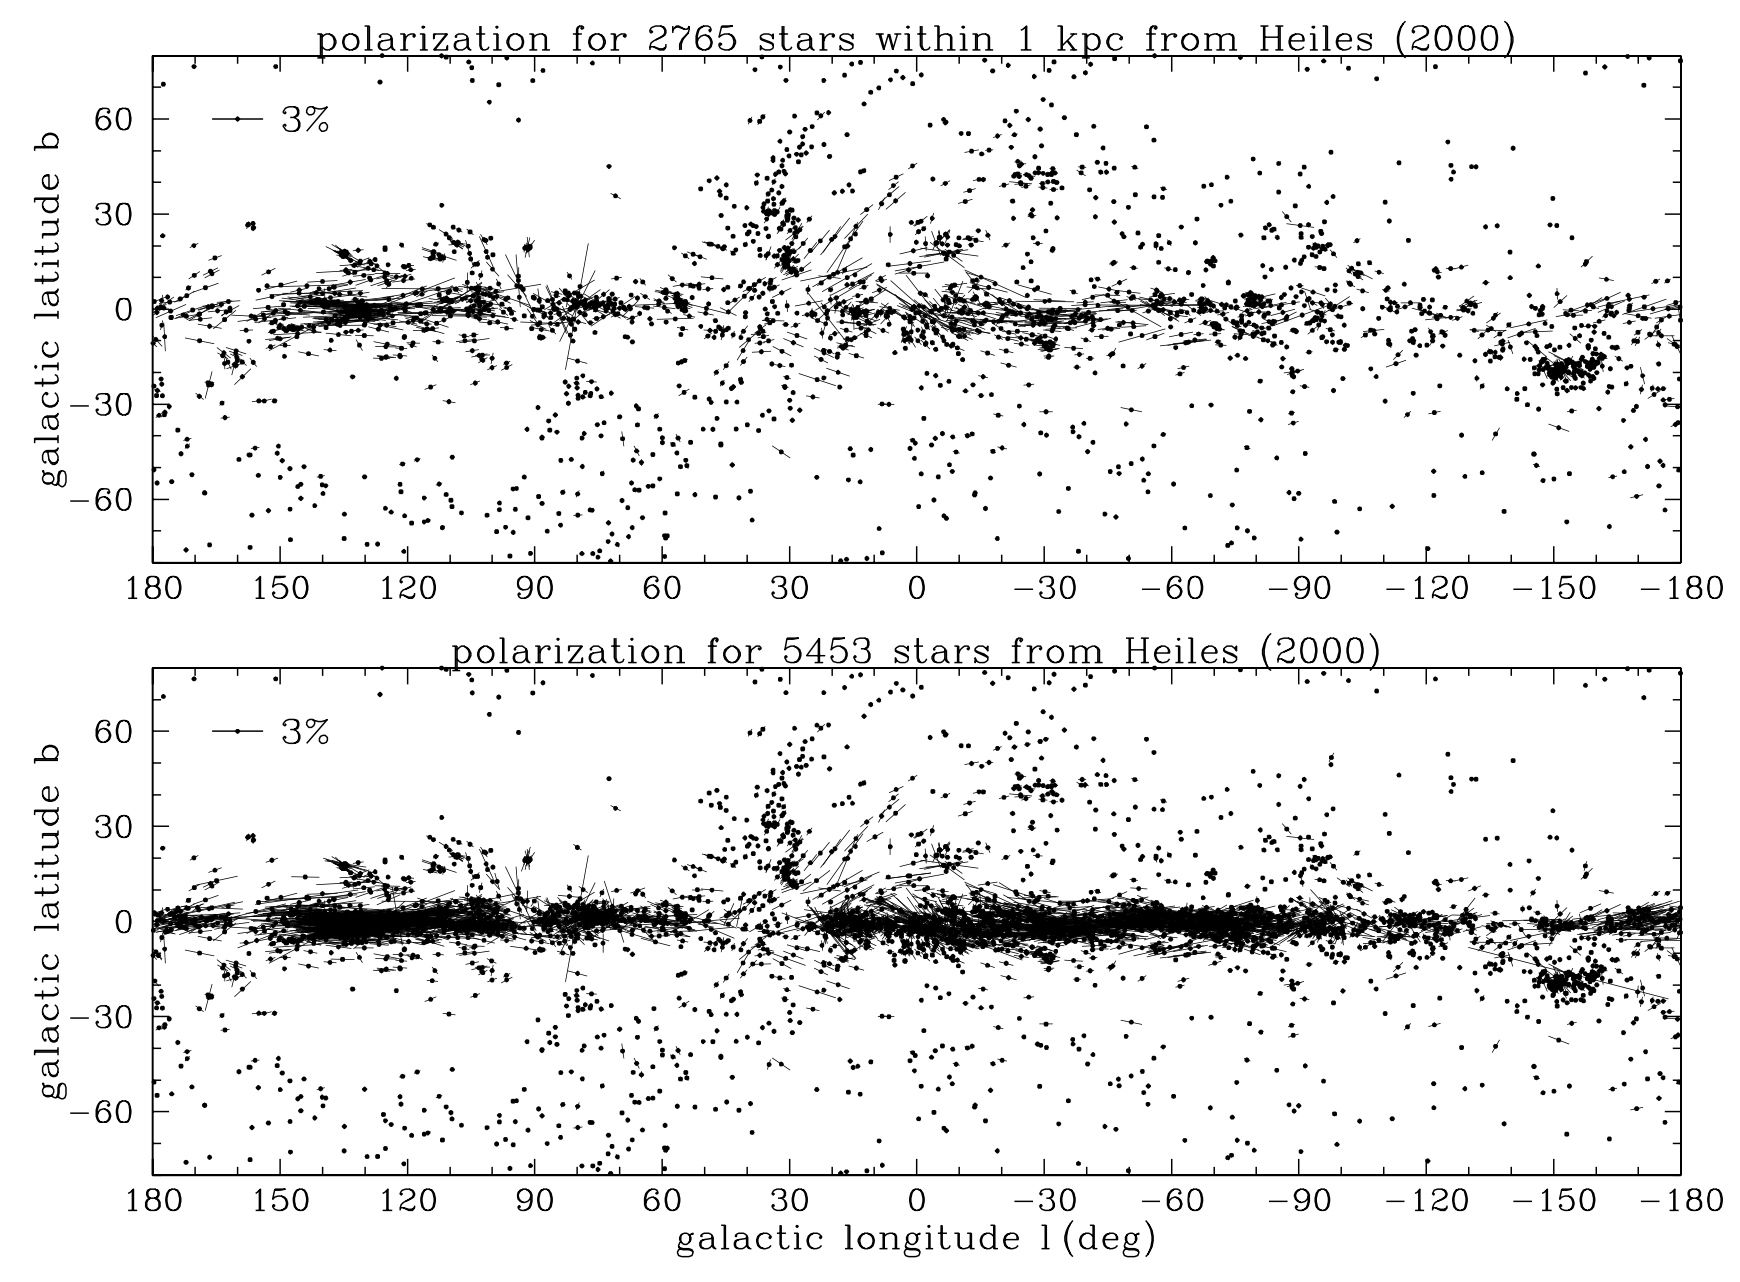
\includegraphics[width=14cm]{figures/starpol.png}
    \caption{\footnotesize{Linear polarization of starlight plotted in galactic coordinates, for stars within $1\,{\rm kpc}$, and for all stars in the catalogue of Heiles (2000). The length of each line segment is proportional to the degree of polarization. Figure taken from Draine (2011).}}
    \label{fig:starpol}
\end{figure}

{\noindent}The polarization percentage typically peaks near the V band ($5,500$\AA), and can be empirically described by the ``Serkowski law'':

\begin{align*}
    p(\lambda) \approx p_\mathrm{max}\exp \left[-K\ln^2\left(\frac{\lambda}{\lambda_\mathrm{max}}\right)\right] ~ [{\rm dimensionless}]
\end{align*}

{\noindent}with $\lambda_\mathrm{max}\approx5500$\AA~and $K\approx1.15$. The peak polarization $p_\mathrm{max}$ is found to fall within an envelope

\begin{align*}
    0 < &p_\mathrm{max} \leq 0.09 \left[\frac{E(B-V)}{{\rm mag}}\right] \approx 0.03\left[\frac{A_V}{{\rm mag}}\right] ~ [{\rm dimensionless}] \\
    0 < &p_V \lesssim 0.03\tau_V ~ [{\rm dimensionless}].
\end{align*}

{\noindent}The polarization is produced by dust grains that are somehow partially aligned by the interstellar magnetic field. It appears that the grains are aligned with their shortest axes tending to be parallel to the magnetic field direction. The largest values of $p_\mathrm{max}/E(B-V)$ are presumed to arise on sightlines where the magnetic field is uniform and perpendicular to the line of sight. While the Serkowski law was originally put forward as an empirical fit to the observed polarization at $0.3\,\mu{\rm m}\lesssim \lambda \lesssim 1\,\mu{\rm m}$, it turns out to give a surprisingly good approximation to the measured linear polarization in the vacuum UV, although there are some sightlines where the Serkowski law under-predicts the UV polarization, and one sightline where the $2175$\AA~feature appears to be weakly polarized.

{\noindent}The mechanism responsible for the grain alignment remains a fascinating puzzle . Independent of the grain alignment mechanism, however, we can infer the sizes of the interstellar grains responsible for this polarization by noting that the extinction rises rapidly into the UV whereas the polarization declines . This can be understood if the grains responsible for the polarization have diameters $2a$ such that $a\approx(\lambda_{\rm max}/2\pi)\approx0.1\,\mu{\rm m}$: as one proceeds into the UV, one moves toward the ``geometric optics'' limit where both polarization modes suffer the same extinction, so the polarization goes to zero. Thus we conclude that:

\begin{itemize}
    \item The extinction at $\lambda\approx0.55\,\mu{\rm m}$ has an appreciable contribution from grains with sizes $a\approx0.1\,\mu{\rm m}$. These grains are non-spherical and substantially aligned.
    \item The grains with $a\lesssim0.05\,\mu{\rm m}$, which dominate the extinction at $\lambda\lesssim0.3\,\mu{\rm m}$, are either spherical (which seems unlikely) or minimally aligned.
\end{itemize}

{\noindent}\textbf{Scattering of Starlight}: When an interstellar cloud happens to be unusually near one or more bright stars, we have a reflection nebula, where we see starlight photons that have been scattered by the dust in the cloud. The spectrum of the light coming from the cloud surface shows the stellar absorption lines, thus demonstrating that scattering rather than some emission process is responsible. By comparing the observed scattered intensity with the estimated intensity of the starlight incident on the cloud, it is possible to infer the albedo $\omega$ of the dust -- the ratio of scattering cross section to extinction cross section. It is also possible to infer $\langle\cos\theta\rangle$ for the dust, where $\theta$ is the scattering angle.

{\noindent}Figure \ref{fig:albedo} shows $\omega$ and $\langle\cos\theta\rangle$ for (1) the dust in the general diffuse ISM producing the ``diffuse galactic light,'' (2) dust in individual clouds illuminated by the general starlight, and (3) dust in clouds that are illuminated by a nearby bright star. In the optical, the interstellar dust mixture has an albedo $\omega\approx0.5$ (scattering is about as important as absorption) and the grains are somewhat forward-scattering, with $\langle\cos\theta\rangle\approx0.5$. Rayleigh scattering by particles small compared to the wavelength has $\langle\cos\theta\rangle\approx0$, so this tells us that the particles dominating the scattering at $\lambda\approx0.6\,\mu{\rm m}$ have $a\gtrsim\lambda/2\pi\approx0.1\,\mu{\rm m}$.

\begin{figure}[t]
    \centering
    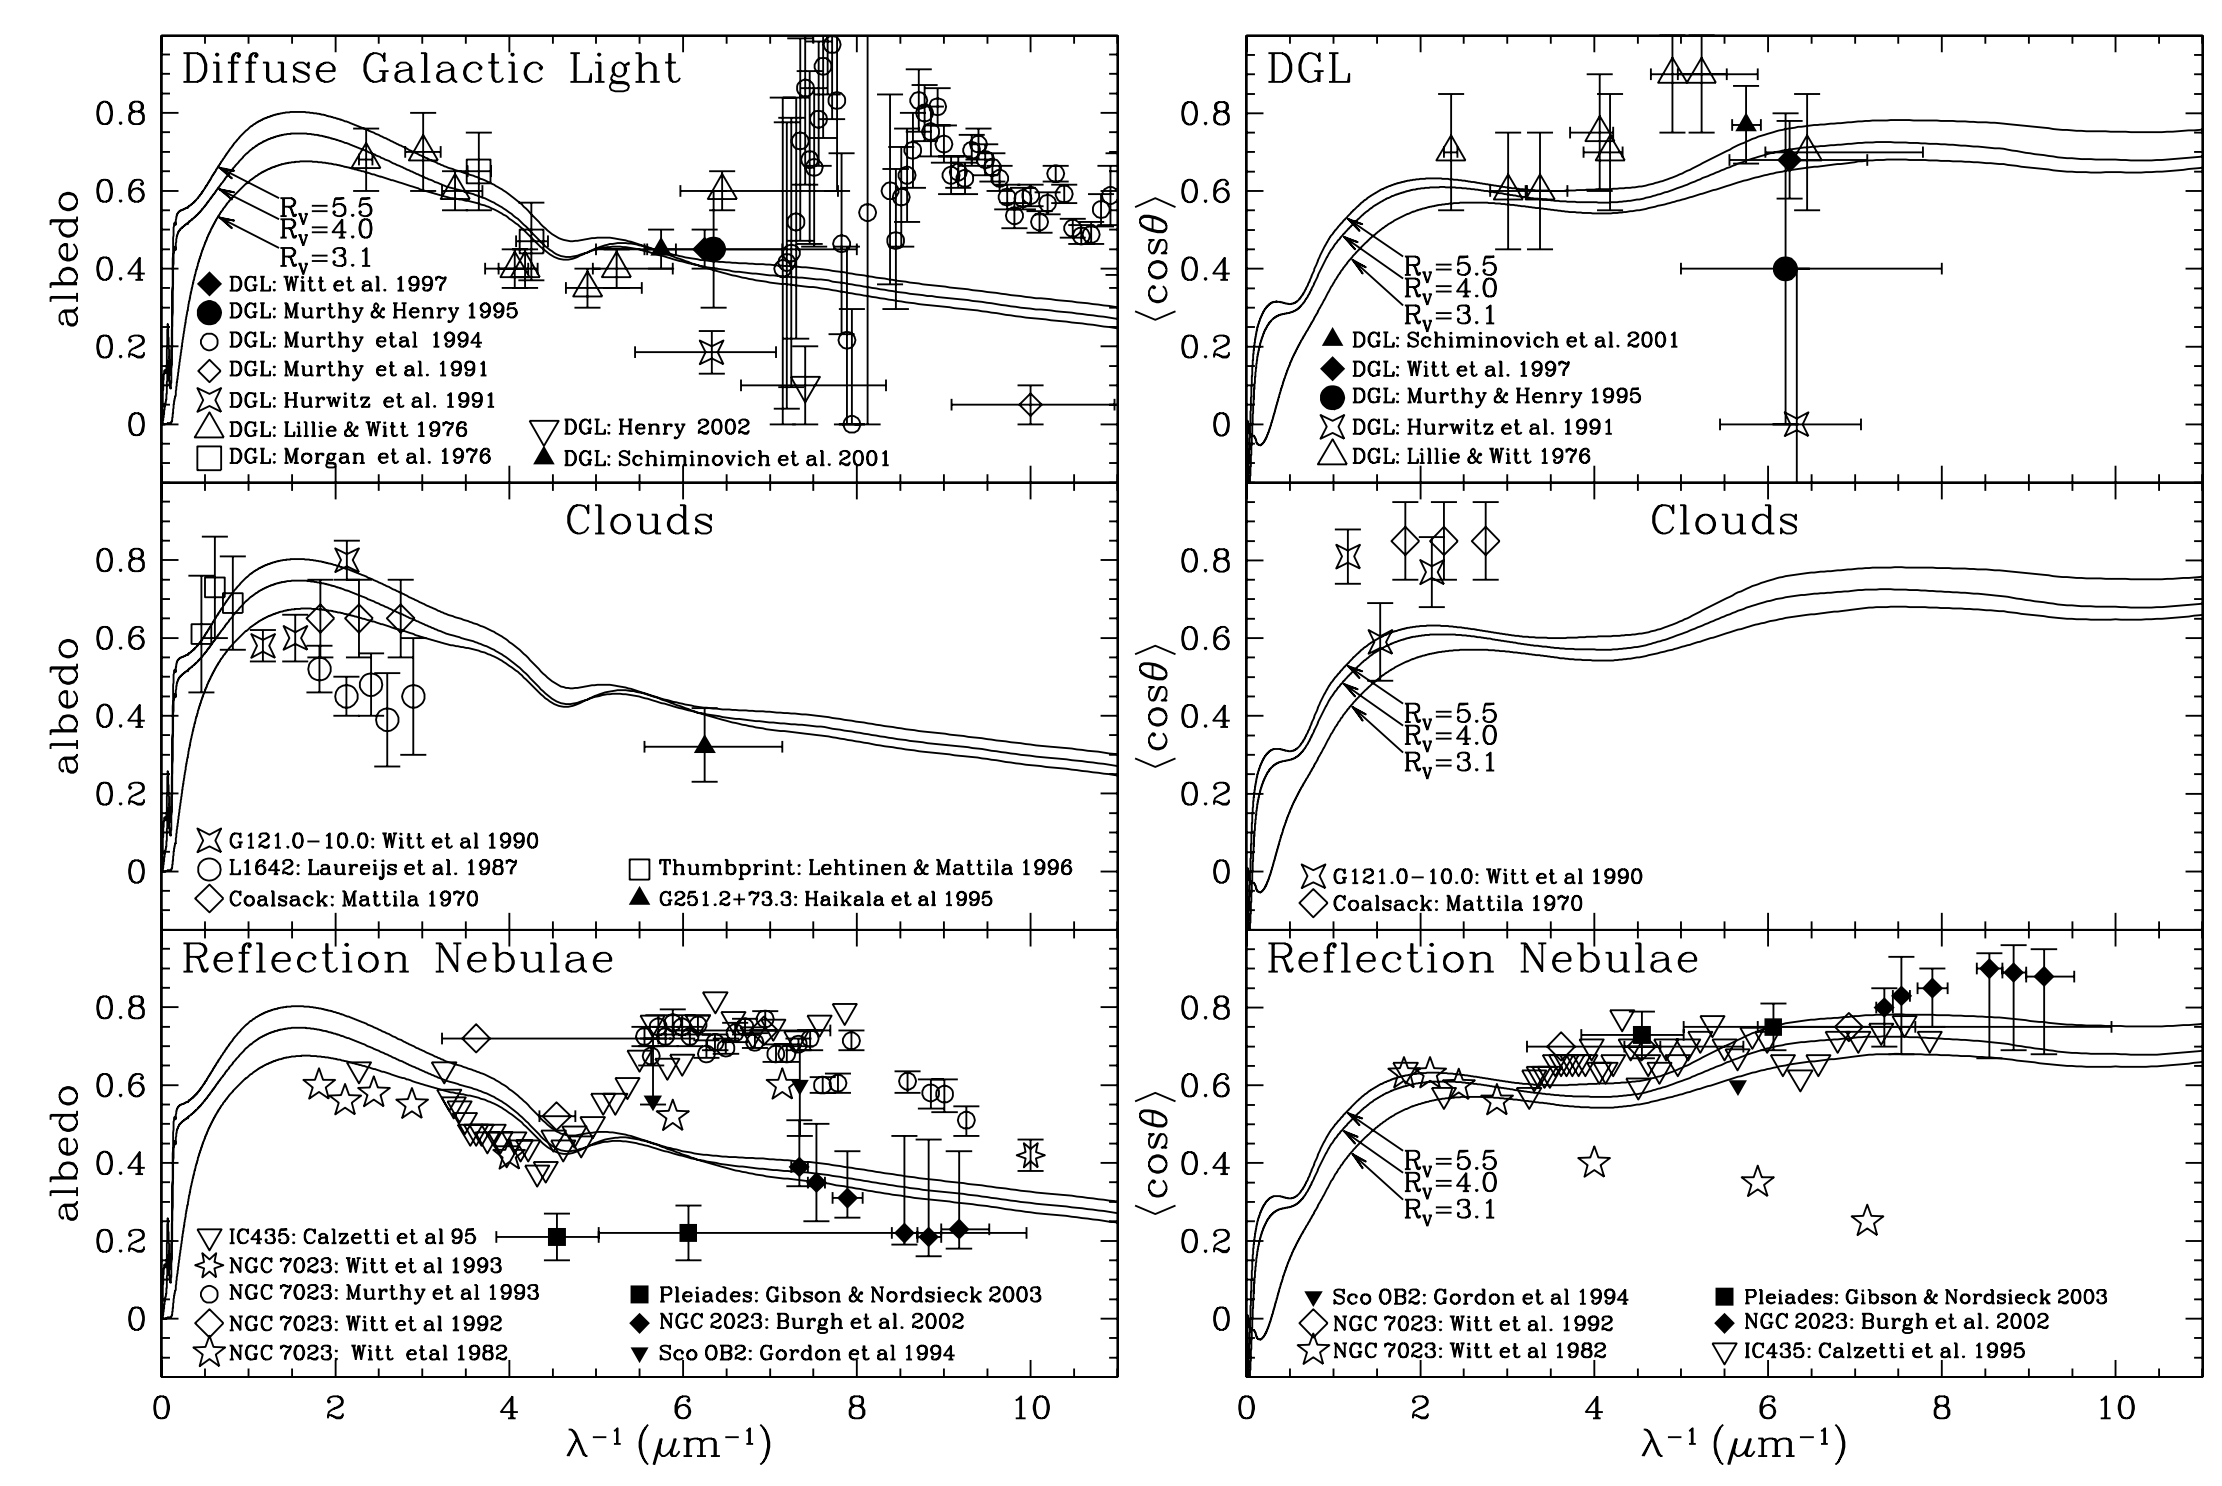
\includegraphics[width=16cm]{figures/albedo.png}
    \caption{\footnotesize{Albedo and scattering asymmetry factor $\langle\cos\theta\rangle$ inferred from observations of the diffuse galactic light, reflection nebulae, and dark clouds. Figure taken from Draine (2011).}}
    \label{fig:albedo}
\end{figure}

{\noindent}\textbf{IR emission}: Dust grains are heated by starlight, and cool by radiating in the IR. The emission from dust at high galactic latitudes has been studied by a number of satellites. Figure \ref{fig:dustir} shows the emission spectrum from $800\,\mu{\rm m}$ to $3\,\mu{\rm m}$. The $3$ to $12\,\mu{\rm m}$ spectrum is estimated from observations of the Galactic plane near $l\approx45^\circ$, if we assume that the ratio of $3$ to $12\,\mu{\rm m}$ emission to the $100\,\mu{\rm m}$ emission is unchanged in going from observations of the Galactic plane to high galactic latitudes. The correlation of the IR emission with HI $21\,{\rm cm}$ emission at high latitudes is used to estimate the power radiated per H nucleon: $5.0\times10^{-24}\,{\rm erg\,s^{-1}\,H^{-1}}$.

\begin{figure}[t]
    \floatbox[{\capbeside\thisfloatsetup{capbesideposition={right,top},capbesidewidth=4cm}}]{figure}[\FBwidth]
    {\caption{\footnotesize{Observed IR emission per H nucleon from dust heated by the average starlight background in the local MW. Crosses: IRAS; squares: COBE-FIRAS; diamonds: COBE-DIRBE; heavy curve: IRTS;. The interpolated dotted line is used to estimate the total power. Figure taken from Draine (2011).}}
    \label{fig:dustir}}
    {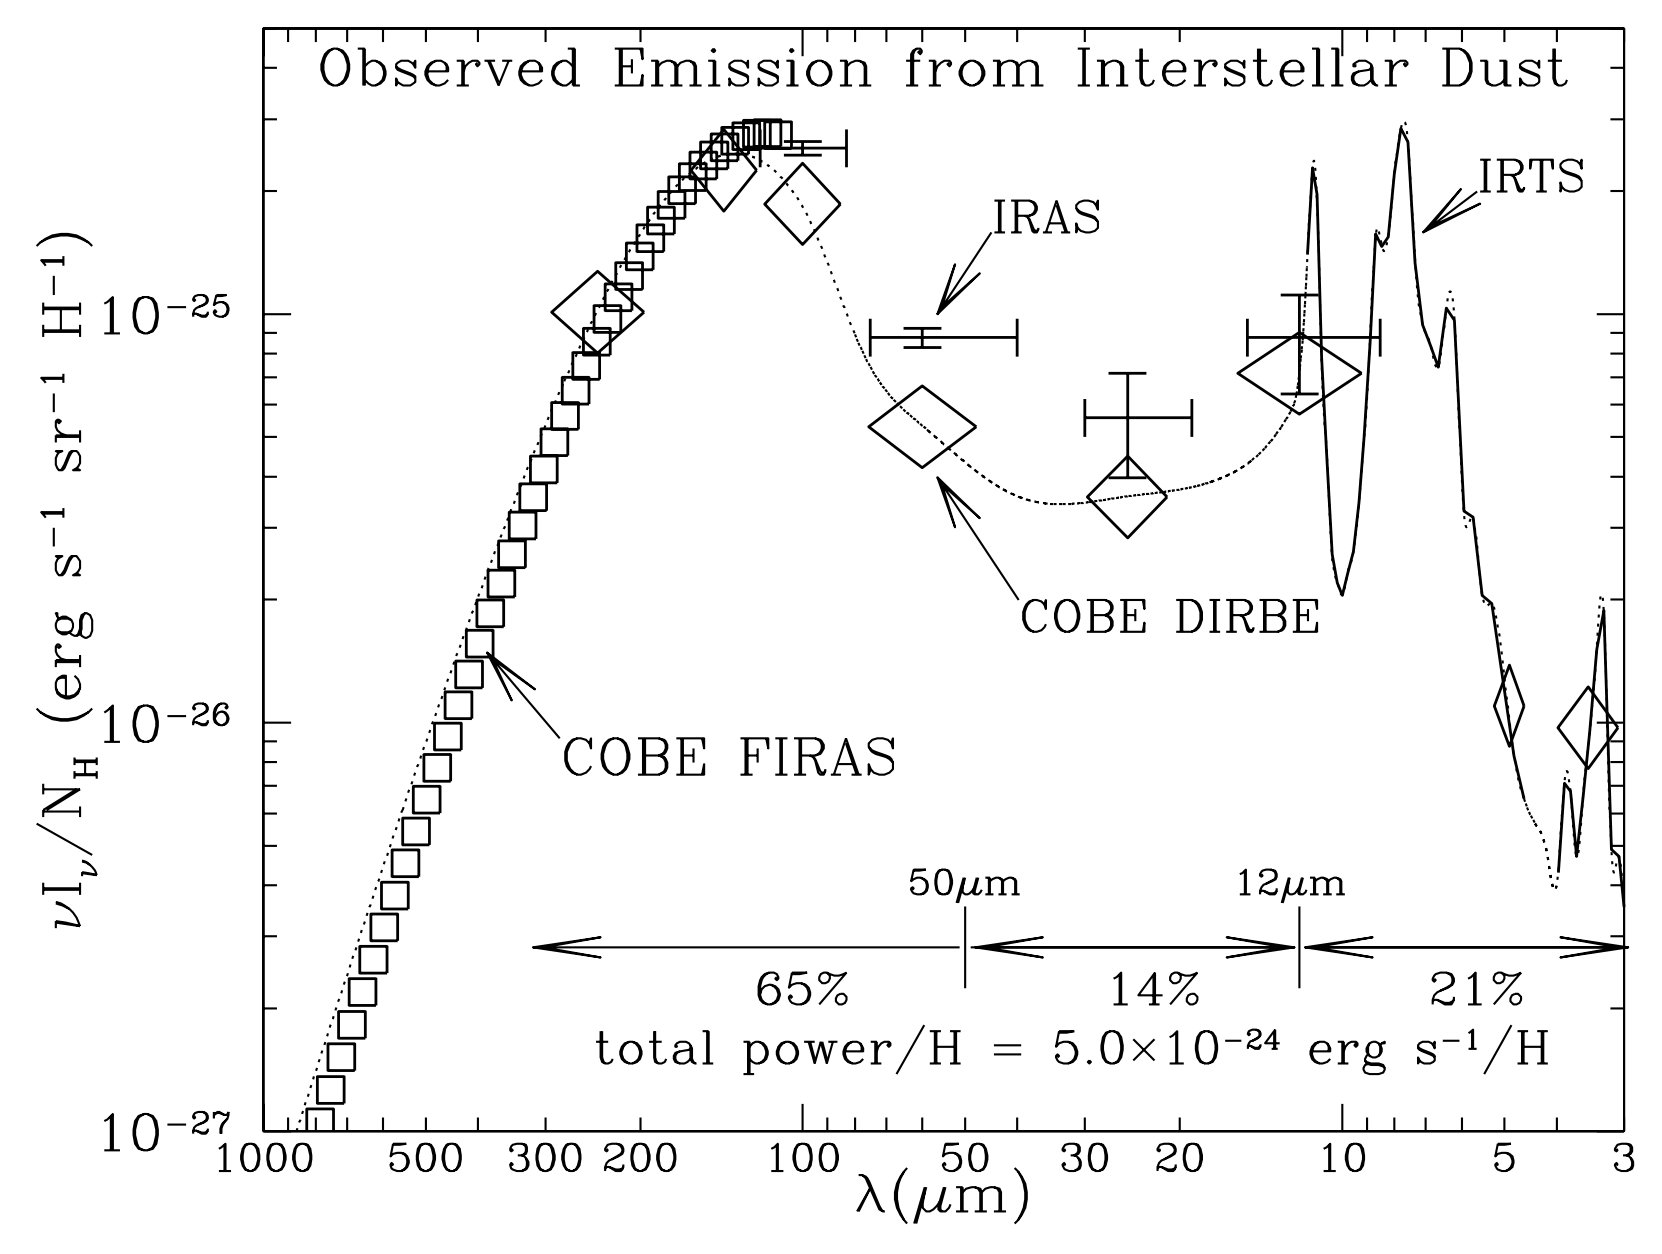
\includegraphics[width=12cm]{figures/dustIR.png}}
\end{figure}

{\noindent}Interstellar dust is heated primarily by starlight, and the total power radiated requires, therefore, that the absorption cross section of interstellar dust be such that the power absorbed per H (for the estimated spectrum of the starlight heating the dust) match the observed emission, $5.0\times10^{-24}\,{\rm erg\,s^{-1}\,H^{-1}}$. The IR spectrum provides very strong constraints on grain models, as the dust must include a component that can account for the fact that $\sim35\%$ of the radiated power is short-ward of $50\,\mu{\rm m}$, including the strong emission features at $\sim12\,\mu{\rm m}$ and $6-8\,\mu{\rm m}$.

{\noindent}\textbf{Luminescence}: The energy absorbed by dust grains is primarily reradiated in the mid- and far-IR, but there is evidence that dust grains also emit light at optical and near-IR wavelengths. Studies of reflection nebulae indicate that there is more light emerging at wavelengths $6000-8000$\AA~than can be accounted for by scattering alone, and this excess is ascribed to luminescence from dust grains following absorption of shorter-wavelength photons. Luminescence at $6000-8000$\AA~is also termed ``extended red emission,'' or ERE. Luminescence in the blue has also been reported. Candidate materials to explain this luminescence must of course reproduce the observed luminescence spectrum. The luminescing materials have not yet been conclusively identified. The blue luminescence may be produced by neutral PAHs, and PAH di-cations (PAH$^{++}$) may be responsible for the ERE.


{\noindent}\textbf{H$_2$ formation}: Molecular hydrogen is a lower energy state than atomic hydrogen, so an isolated box of hydrogen left for an infinite amount of time will eventually become predominantly molecular. In interstellar space, though, the atomic versus molecular fraction in a gas is determined by a balance between formation and destruction processes.

{\noindent}Atomic hydrogen can turn into molecular hydrogen in the gas phase, but this process is extremely slow. This is ultimately due to the symmetry of the hydrogen molecule. To form an H$_2$ molecule, two H atoms must collide and then undergo a radiative transition that removes enough energy to leave the resulting pair of atoms in a bound state. However, two H atoms that are both in the ground state constitute a symmetric system, as does an H$_2$ molecule in its ground state. Because both the initial and final states are symmetric, one can immediately show from symmetry considerations that the system cannot emit dipole radiation.

{\noindent}Due to this limitation, the dominant formation process is instead formation on the surfaces of dust grains. In this case the excess energy released by forming the molecule is transferred into vibrations in the dust grain lattice, and there is no need for forbidden photon emission.

{\noindent}\textbf{Composition of interstellar dust}: There is ample evidence for the presence of substantial amounts of submicron-sized dust particles in interstellar space. What is this dust made of? This question has been difficult to answer.

{\noindent}The preferred approach would be spectroscopy: ideally, we would observe spectroscopic features that would uniquely identify the materials, and, furthermore, allow us to measure the amounts of each material present. This is the approach that is followed for atoms, ions, and small molecules, but unfortunately it is difficult to apply to solid materials because: (1) the optical and UV absorption is largely a continuum; and (2) the spectral features that do exist are broad, making them difficult to identify conclusively.

{\noindent}An alternative approach is to ask: what materials could plausibly be present in the ISM in quantities sufficient to account for the observed extinction? A Kramers-Kronig integral over the observed extinction indicates that the total grain mass relative to total hydrogen mass $M_{\rm dust}/M_{\rm H}\gtrsim0.0083$.

{\noindent}Additionally, certain elements appear to be underabundant, or ``depleted,'' in the gas phase; observed depletions can tell us about the major elemental composition of interstellar dust. The available evidence indicates that the overall abundances in the ISM are close to the values in the solar photosphere. Because there is no way to have hydrogen contribute appreciably to the grain mass (even polyethylene $(C{\rm H}_2)_n$ is 86\% carbon by mass), and He and Ne are chemically inert, the only way to have a dust/H mass ratio of $0.0056$ or higher is to build the grains out of the most abundant condensible elements: C, O, Mg, Si, S, and Fe.

{\noindent}With the elements providing the bulk of the grain volume identified, we can limit consideration to the following possible materials:

\begin{itemize}
    \item Silicates (e.g., pyroxene composition or olivine composition)
    \item Oxides of silicon, magnesium, and iron (e.g., SiO$_2$, MgO, Fe$_3$O$_4$)
    \item Carbon solids (graphite, amorphous carbon, and diamond)
    \item Hydrocarbons (e.g., PAHs)
    \item Carbides, particularly silicon carbide (SiC)
    \item Metallic Fe
\end{itemize}

{\noindent}Other elements (e.g., Ti, Cr) are also present in interstellar grains, but, because of their low abundances, they contribute only a minor fraction of the grain mass.

{\noindent}\textbf{The sources of dust grains}: It is apparent that even though dust grains make up only about one percent of the mass of the ISM, they are important constituents in determining its chemistry and physics. The question of the source of these grains then naturally arises. Although observations indicate that grains can be formed in the enveloped of very cool stars, aided by the enhanced density in those environments relative to molecular clouds, grains can also be easily destroyed by UV and X-ray photons. Dust grains are also formed as a product of SN explosions and stellar winds. However, none of these sources appear to be able to provide the abundance of massive grains found in molecular clouds. Rather, it appears that grains probably grow by a process of coagulation within the molecular clouds themselves. Dust grain formation represents just one of many active areas of research into the nature of dust grains and ISM physics.

\subsubsection{Follow-up Questions}

\begin{itemize}
    \item Why is molecular hydrogen (H$_2$) so difficult to detect?
    \item What are other ways in which molecular cloud cores cool?
\end{itemize}

% --------------------------------------------------------------
%               6. 
% --------------------------------------------------------------

\newpage
\subsection{Question 6}

The ISM mainly consists of hydrogen and helium, which are very poor coolants. How, then, do molecular cloud cores ever manage to lose enough heat to collapse and form stars? Why are H
and He such poor coolants?

\subsubsection{Short answer}

Answer.

\subsubsection{Additional context}

{\noindent}\textbf{Cooling of atomic gas:}

{\noindent}Most of the interstellar gas in the Milky Way is neutral, and $\sim78\%$ of the neutral hydrogen is atomic, or HI. The most abundant elements in the Universe after H and He are O, C, and N. Just as in the bulk of the ISM hydrogen is mostly H, in the bulk of the ISM the oxygen is mostly O and the carbon is mostly C$^+$. It's C$^+$ rather than C because the ionization potential of carbon is less than that of hydrogen, and as a result it tends to be ionized by starlight.

{\noindent}An example of the ``\textbf{cooling function}'' $\Lambda$ for predominantly neutral gas, as a function of temperature, is shown in Figure \ref{fig:coolingfunction_HI} for abundances appropriate to diffuse HI in the Milky Way, and for two different fractional ionizations: $x_e=0.017$ (WNM conditions) and $x_e=4\times10^{-4}$ (CNM conditions). For $10\lesssim T\lesssim10^4\,{\rm K}$, the [CII]$158\,\mu{\rm m}$ fine structure line is a major coolant. The [OI]$63\,\mu{\rm m}$ fine structure line is important for $T\gtrsim100\,{\rm K}$. Lyman$\alpha$ cooling dominates only at $T\gtrsim1\times10^4{\rm K}$. 

{\noindent}The critical densities for [CII]$158\,\mu{\rm m}$ and [OI]$63\,\mu{\rm m}$ are $\sim4\times10^3\,{\rm cm^{-3}}$ and $\sim10^5\,{\rm cm^{-3}}$, respectively, implying that collisional de-excitation of these levels is unimportant in the diffuse ISM of the MW. Thus, for fixed composition (and ionization fraction $x_e$), the cooling power per volume $\Lambda\propto n_{\rm H}^2\times\lambda(T)$, where the cooling rate coefficient $\lambda$ depends only on $T$.

\begin{figure}[h!]
    \centering
    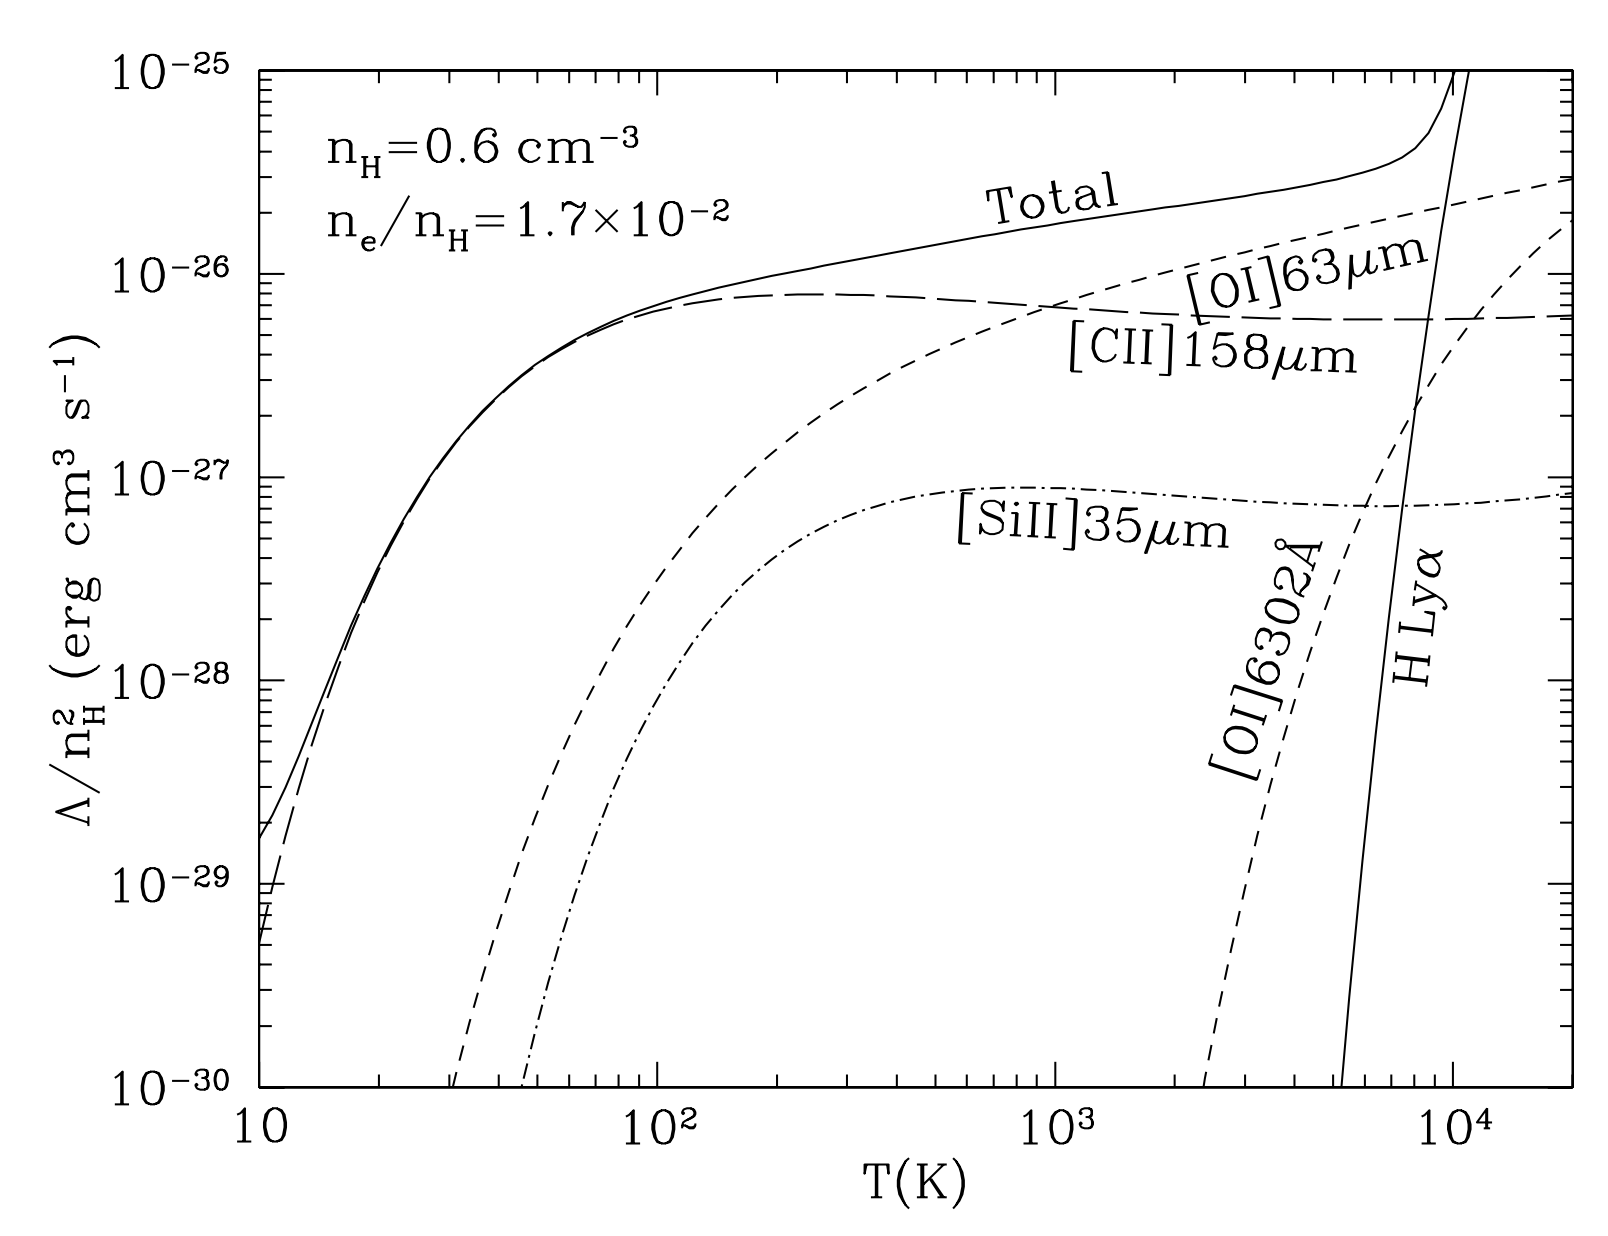
\includegraphics[width=7.5cm]{figures/CoolingFunction_HI_top.png} 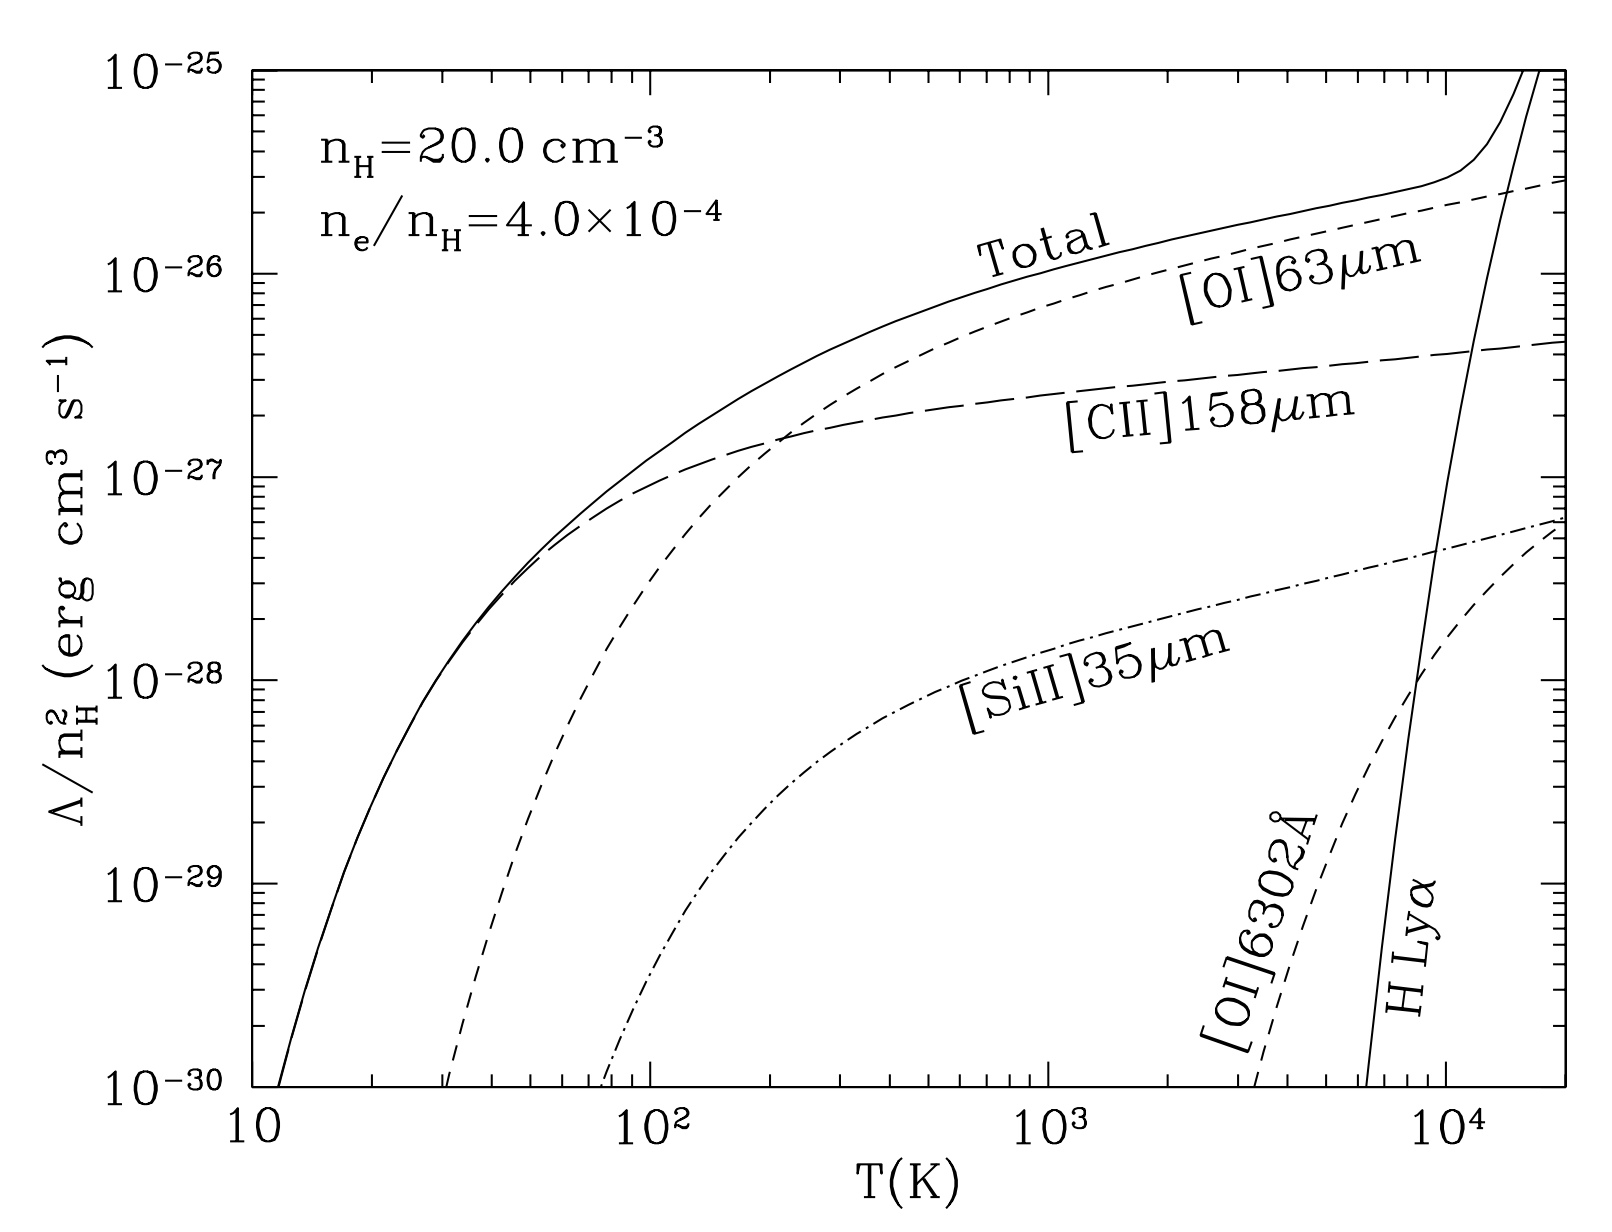
\includegraphics[width=7.5cm]{figures/CoolingFunction_HI_bottom.png}
    \caption{\footnotesize{Cooling rate for neutral HI gas at temperatures $10\lesssim T\lesssim2\times10^4\,{\rm K}$ for two fractional ionizations. For $T<10^4\,{\rm K}$, the cooling is dominated by two fine structure lines: [CII]$158\,\mu{\rm m}$ and [OI]$63\,\mu{\rm m}$. Figure taken from Draine (2011).}}
    \label{fig:coolingfunction_HI}
\end{figure}

{\noindent}\textbf{Cooling of molecular gas:}

{\noindent}At the high densities where stars form, hydrogen tends to be molecular rather than atomic, and H$_2$ very rarely emits radiation via de-excitation. To understand why, we can look at an energy level diagram for rotational levels of H$_2$ (Figure \ref{fig:Henergies}). A diatomic molecule like H$_2$ has three types of excitation: \textbf{electronic} (corresponding to excitations of one or more of the electrons), \textbf{vibrational} (corresponding to vibrational motion of the two nuclei), and \textbf{rotational} (corresponding to rotation of the two nuclei about the center of mass). Generally electronic excitations are highest in energy scale, vibrational are next, and rotational are the lowest in energy.

\begin{figure}[h]
    \floatbox[{\capbeside\thisfloatsetup{capbesideposition={right,top},capbesidewidth=4cm}}]{figure}[\FBwidth]
    {\caption{\footnotesize{Level diagram for the rotational levels of para- and ortho-H$_2$, showing the energy of each level. Level data are taken from \href{http://www.gemini.edu/sciops/instruments/nir/wavecal/h2lines.dat}{http://www.gemini.edu/sciops\\/instruments/nir/wavecal\\/h2lines.dat}. Figure taken from Draine (2011).}}
    \label{fig:Henergies}}
    {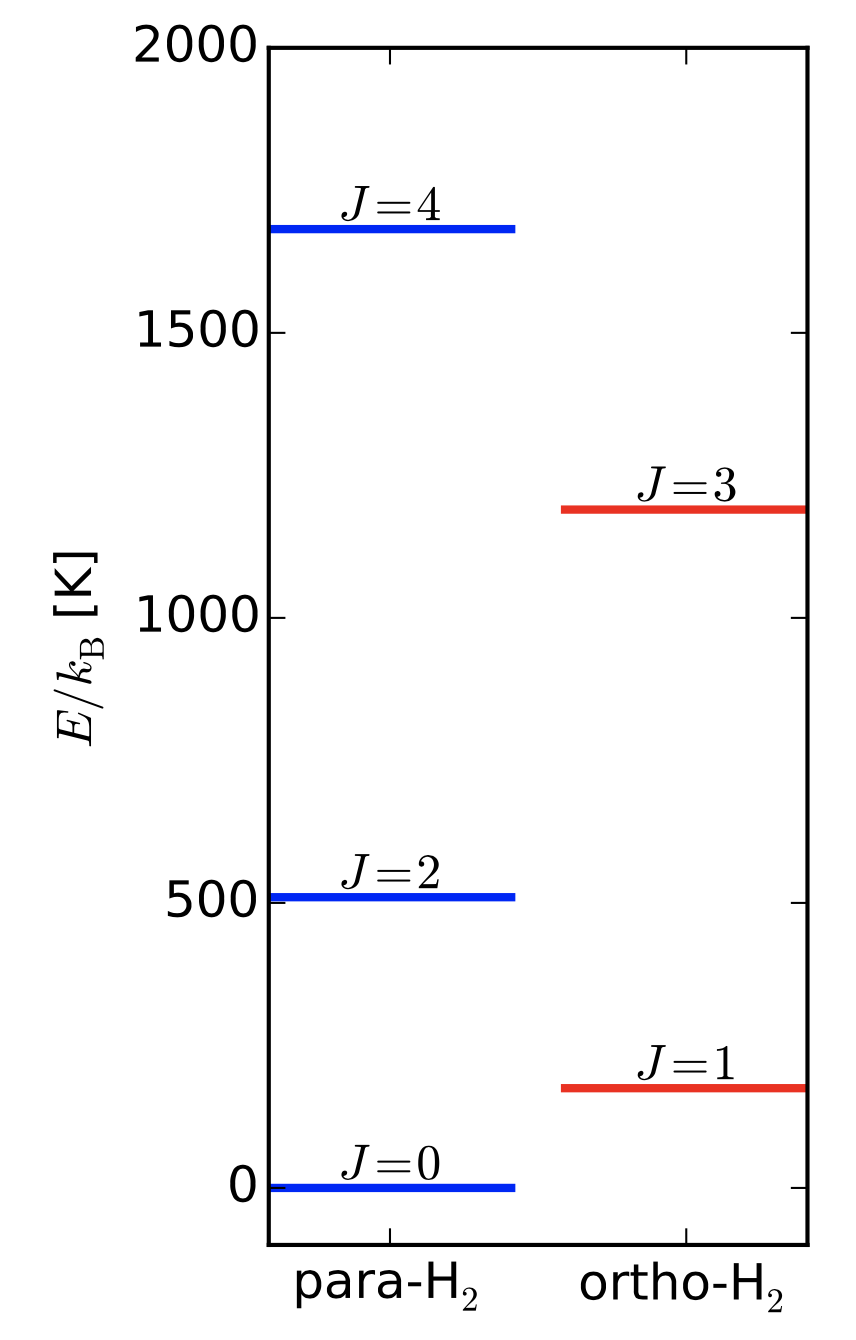
\includegraphics[width=5cm]{figures/Henergies.png}}
\end{figure}

{\noindent}For H$_2$, the first thing to notice is that the first excited state, the $J=1$ rotational state, is $175\,{\rm K}$ above the ground state. Since the dense ISM where molecules form is often also cold, $T\sim10\,{\rm K}$, almost no molecules will be in this excited state. However, it gets even worse: H$_2$ is a \textbf{homonuclear molecule}, and for reasons of symmetry $\Delta J=1$ radiative transitions are forbidden in homonuclear molecules. Indeed, there is no electronic process by which a hydrogen molecule with odd $J$ to turn into one with even $J$, and vice versa, because the allowed parity of $J$ is determined by the spins of the hydrogen nuclei. We refer to the even $J$ state as \textbf{para-H}$\mathbf{_2}$, and the odd $J$ state as \textbf{ortho-H}$\mathbf{_2}$.

{\noindent}The significance of this is that \textit{there is no $J=1\rightarrow0$ emission}. Instead, the lowest-lying transition is the $J=2\rightarrow0$ quadrupole. This is very weak, because it's a quadrupole. More importantly, however, the $J=2$ state is $510\,{\rm K}$ above the ground state. This means that, for a population in equilibrium at a temperature of $10\,{\rm K}$, the fraction of molecules in the $J=2$ state is $\sim e^{-510/10}\approx10^{-22}$! In effect, in a molecular cloud there are simply no H$_2$ molecules in states capable of emitting and therefore cannot cool the gas. The very high temperature required to excite the H$_2$ molecular is its low mass: for a quantum oscillator or rotor the level spacing varies with reduced mass as $m^{-1/2}$. It is the low mass of the hydrogen atom that creates our problems.

{\noindent}In molecular clouds there are two main cooling processes: molecular lines and dust radiation. Dust can cool the gas efficiently because dust grains are solids, so they are thermal emitters. However, dust is only able to cool the gas if collisions between dust grains and hydrogen molecules occur often enough to keep them thermally well-coupled. Otherwise the grains cool off, but the gas stays hot. The density at which grains and gas become well-coupled is around $10^4-10^5\,{\rm cm^{-3}}$ which is higher than the typical density in a GMC.

{\noindent}The remaining cooling process is line emission, and by far the most important molecule for this purpose is CO. H$_2$ is the dominant species in molecular regions, but it is very hard to observe directly -- the temperatures are too low for it to be excited. Moreover, H$_2$ is also not the dominant coolant for the same reason. Instead, that role falls to the CO molecule. The physics is fairly simple. CO molecules are excited by inelastic collisions with hydrogen molecules, and such collisions convert kinetic energy to potential energy within the molecule. If the molecule de-excites radiatively, and the resulting photon escapes the cloud, the cloud loses energy and cools.


% --------------------------------------------------------------
%               7. 
% --------------------------------------------------------------

\newpage
\subsection{Question 7}

The stars in the solar neighbourhood, roughly the $300\,\mathrm{pc}$ around us, have a range of ages, metallicities and orbital properties. How are those properties related?

\subsubsection{Short answer}

Answer.

\subsubsection{Additional context}

{\noindent}\textbf{Age-metallicity relation:} Assuming that at the beginning of its evolution the MW had a chemical composition with only low metal content, the metallicity should be strongly related to the age of a stellar population. With each new generation of stars, more metals are produced and ejected into the ISM, partially by stellar winds, but mainly by SN explosions. Stars that are formed later should therefore have a higher metal content than those that were formed in the early phase of the Galaxy. One would thus expect that a relation exists between the age of a star and its metallicity.

{\noindent}For instance, under this assumption the iron abundance [Fe/H] can be used as an age indicator for a stellar population, with the iron predominantly being produced and ejected in SNe of Type Ia. Therefore, a newly formed generation of stars has a higher fraction of iron than their predecessors, and the youngest stars should have the highest iron abundance. Indeed one finds [Fe/H]$=4.5$ (i.e., $3\times10^{-5}$ of the Solar iron abundance) for extremely old stars, whereas very young stars have [Fe/H]$=1$, so their metallicity can significantly exceed that of the Sun.

{\noindent}However, this age-metallicity relation is not very tight. On the one hand, SNe Ia occur only $\gtrsim10^9\,{\rm yr}$ after the formation of a stellar population. The exact time-span is not known because even if one accepts the accretion scenario for SN Ia described above, it is unclear in what form and in what systems the accretion of material onto the white dwarf takes place and how long it typically takes until the limiting mass is reached. On the other hand, the mixing of the SN ejecta in the ISM occurs only locally, so that large inhomogeneities of the [Fe/H] ratio may be present in the ISM, and thus even for stars of the same age. An alternative measure for metallicity is [O/H], because oxygen is produced and ejected mainly in supernova explosions of massive stars. These happen just $\sim10^7\,{\rm yr}$ after the formation of a stellar population, which is virtually instantaneous.

{\noindent}\textbf{Velocity dispersion of stars:} The dispersion of stellar velocities relative to the LSR can be determined, i.e., the mean square deviation of their velocities from the velocity of the LSR. For young stars (A stars, for example), this dispersion happens to be small. For older K giants it is larger, and is larger still for old, metal-poor red dwarf stars. We observe a very well-defined velocity-metallicity relation which, when combined with the age-metallicity relation, suggests that the oldest stars have the highest peculiar velocities. This effect is observed in all three coordinates and is in agreement with the relation between the age of a stellar population and its scale-height, the latter being linked to the velocity dispersion via $\sigma_z$.

{\noindent}\textbf{Stellar populations:} The chemical composition of stars in the thin and the thick disks differs: we observe the clear tendency that stars in the thin disk have a higher metallicity than those in the thick disk. In contrast, the metallicity of stars in the Galactic halo and in the bulge is smaller. To paraphrase these trends, one distinguishes between stars of population I (pop I) which have a Solar-like metallicity ($Z\sim0.02$) and are mainly located in the thin disk, and stars of population II (pop II) that are metal-poor ($Z\sim0.001$) and predominantly found in the thick disk, in the halo, and in the bulge. In reality, stars cover a wide range in $Z$, and the figures above are only characteristic values. For stellar populations a somewhat finer separation was also introduced, such as ``extreme population I'', ``intermediate population II'', and so on. The populations also differ in age (stars of pop I are younger than those of pop II), in scale height (as mentioned above), and in the velocity dispersion perpendicular to the disk ($\sigma_z$ is larger for pop II stars than for pop I stars).

{\noindent}\textbf{Stellar age distribution in the bulge:} The stars in the bulge cover a large range in metallicity,$-1\lesssim {\rm [Fe=H]} \lesssim0.6$, with a mean of about $0.3$, i.e., the mean metallicity is about twice that of the Sun. The metallicity also changes as a function of distance from the center, with more distant stars having a smaller value of [Fe/H]. 

{\noindent}The high metallicity means that either the stars of the bulge formed rather late, according to the age-metallicity relation, or that it is an old population with very intense star formation activities at an early cosmic epoch. We can distinguish between these two possibilities from the chemical composition of stars in the bulge, obtained from spectroscopy. Bulge stars have a significantly higher abundance of Mg, relative to iron, than the stars from the thin disk, but much more similar to thick disk stars. This implies that the enrichment must have occurred predominantly by core-collapse supernovae, since they produce a high ratio of elements like magnesium compared to iron, whereas Type Ia SNe produce mainly iron-group elements. Therefore, most of the bulge stars must have formed before the Type Ia SNe exploded. Whereas the time lag between the birth of a stellar population and the explosion of the bulk of Type Ia SN is not well known (it depends on the evolution of binary systems), it is estimated to be between $1$ and $3\,{\rm Gyr}$. Hence, most of the bulge stars must have formed on a rather short time-scale: the bulge consists mainly of an old stellar population, formed within $\sim1\,{\rm Gyr}$.

% --------------------------------------------------------------
%               8. 
% --------------------------------------------------------------

\newpage
\subsection{Question 8}

What are the main sources of heat in the interstellar medium?

\subsubsection{Short answer}

Possible mechanisms for heating HI regions include:

\begin{itemize}
    \item Ionization by cosmic rays
    \item Photoionization of H and He by x rays
    \item Photoionization of dust grains by starlight UV
    \item Photoionization of C, Mg, Si, Fe, etc., by starlight UV
    \item Heating by shock waves and other MHD phenomena
\end{itemize}

\subsubsection{Additional context}

{\noindent}\textbf{Ionization by cosmic rays:} The great advantage of cosmic rays over FUV photons is that, because they are relativistic particles, they have much lower interaction cross sections, and thus are able to penetrate into regions where light cannot. The process of cosmic ray heating works as follows. The first step is the interaction of a cosmic ray with an electron, which knocks the electron off a molecule:

\begin{align*}
    {\rm CR + H_2 \rightarrow H_2^+ + e^- + CR}.
\end{align*}

{\noindent}The free electron's energy depends only weakly on the CR's energy, and is typically $\sim30\,{\rm eV}$.

{\noindent}The electron cannot easily transfer its energy to other particles in the gas directly, because its tiny mass guarantees that most collisions are elastic and transfer no energy to the impacted particle. However, the electron also has enough energy to ionize or dissociate other hydrogen molecules, which provides an inelastic reaction that can convert some of its $\sim30\,{\rm eV}$ to heat. Secondary ionizations do indeed occur, but in this case almost all the energy goes into ionizing the molecule ($15.4\,{\rm eV}$), and the resulting electron has the same problem as the first one: it cannot effectively transfer energy to the much more massive protons. Instead, there are a number of other channels that allow electrons to dump their energy into motion of protons.

{\noindent}\textbf{Photoionization of dust grains by starlight UV:} The dominant heating process in the atomic ISM is the \textbf{grain photoelectric effect}: photons from stars with energies of $\sim8-13.6\,{\rm eV}$ hit dust grains and eject fast electrons via the photoelectric effect. The fast electrons then thermalize and deposit their energy as heat in the gas. The rate per H nucleus at which this process deposits energy can be written approximately as

\begin{align*}
    \Gamma_{\rm PE} \approx 4.0\times10^{-26}\chi_{\rm FUV}Z_d'e^{-\tau_d} ~ [{\rm erg\,s^{-1}}],
\end{align*}

{\noindent}where $\chi_{\rm FUV}$ is the intensity of the FUV radiation field scaled to its value in the Solar neighborhood, $Z_d'$ is the dust abundance scaled to the Solar neighborhood value, and $\tau_d$ is the dust optical depth to FUV photons. The result is, not surprisingly, proportional to the radiation field strength (and thus the number of photons available for heating), the dust abundance (and thus the number of targets for those photons),and the $e^{-\tau_d}$ factor by which the radiation field is attenuated.

{\noindent}At FUV wavelengths, typical dust opacities are $\kappa_d\approx500\,{\rm cm^2\,g^{-1}}$, so at a typical molecular cloud surface density $\Sigma\approx50-100\,{\rm M_\odot\,pc^2}$, $\tau_d\sim5-10$, and thus $e^{-\tau_d}\approx10^{-3}$. Thus in the interiors of molecular clouds, photoelectric heating is strongly suppressed simply because the FUV photons cannot get in. Typical photoelectric heating rates are therefore of order a few $10^{29}\,{\rm erg\,s^{-1}}$ per H atom deep in cloud interiors, though they can obviously be much larger at cloud surfaces or in regions with stronger radiation fields.

{\noindent}\textbf{Shocks:} Before discussing individual feedback mechanisms in detail, it is also helpful to lay out two general categories that can be used to understand them. Let us consider a population of stars surrounded by initially-uniform interstellar gas. Those stars eject both photons and baryons (in the form of stellar winds) into the surrounding gas, and these photons and baryons carry both momentum and energy. We want to characterize how the ISM will respond. One important consideration is that it is very hard to raise the temperature of molecular gas (or even dense atomic gas) because it is able to radiate so efficiently. A factor of 10 increase in the radiative heating rate might yield only a tens of percent increase in temperature. This is true as long as the gas is cold and dense, but at sufficiently high temperatures or if the gas is continuously illuminated then the cooling rate begins to drop off, and it is possible for gas to remain hot.

{\noindent}A critical distinction is therefore between mechanisms that are able to keep the gas hot for a time that is long enough to be significant (generally of order the crossing time of the cloud or longer), and those where the cooling time is much shorter. For the latter case, the energy delivered by the photons and baryons will not matter, only the momentum delivered will. The momentum cannot be radiated away. We refer to feedback mechanism where the energy is lost rapidly as momentum-driven feedback, and to the opposite case where the energy is retained for at least some time as energy-driven, or explosive, feedback. 

{\noindent}To understand why the distinction between the two is important, let us consider two extreme limiting cases. We place a cluster of stars at the origin and surround it by a uniform region of gas with density $\rho$. At time $t=0$, the stars ``turn on'' and begin emitting energy and momentum, which is then absorbed by the surrounding gas. Let the momentum and energy injection rates be $\dot{p}_w$ and $\dot{E}_w$; it does not matter if the energy and momentum are carried by photons or baryons, so long as the mass swept up is significantly greater than the mass carried by the wind.

{\noindent}The wind runs into the surrounding gas and causes it to begin moving radially outward, which in turn piles up material that is further away, leading to an expanding shell of gas. Now let us compute the properties of that shell in the two extreme limits of all the energy being radiated away, and all the energy being kept. If all the energy is radiated away, then at any time the radial momentum of the shell must match the radial momentum injected up to that time, i.e.,

\begin{align*}
    p_{\rm sh} = M_{\rm sh}v_{\rm sh} = \dot{p}_{\rm sh}t ~ [{\rm kg\,m\,s^{-1}}].
\end{align*}

{\noindent}The kinetic energy of the shell is

\begin{align*}
    E = \dot{p}_{\rm sh}^2 2M_{\rm sh} = \frac{1}{2}v_{\rm sh}\dot{p}_wt ~ [{\rm J}].
\end{align*}

{\noindent}For comparison, if none of the energy is radiated away, the energy is simply

\begin{align*}
    E = \dot{E}_wt ~ [{\rm J}].
\end{align*}

{\noindent}Thus the energy in the energy-conserving case is larger by a factor of

\begin{align*}
    \frac{1}{v_{\rm sh}}\cdot\frac{2\dot{E}_w}{\dot{p}_w}.
\end{align*}

{\noindent}If the energy injected by the stars is carried by a wind of baryons, then $2\dot{E}_w/\dot{p}_w$ is simply the speed of that wind, while if it is carried by photons, then $2\dot{E}_w/\dot{p}_w=2c$. Thus the energy in the energy-conserving case is larger by a factor of $2c/v_{sh}$ for a photon wind, and $v_w/v_{\rm sh}$ for a baryon wind. These are not small factors: observed expanding shells typically have velocities of at most a few tens of $km\,s^{-1}$, while wind speeds from massive stars, for example, can be thousands of $km\,s^{-1}$. Thus it matters a great deal where a particular feedback mechanism lies between the energy- and momentum-conserving limits.

{\noindent}Momentum-driven feedback mechanisms include radiation pressure (probably, since the majority of the radiant energy deposited in the ISM will be re-radiated immediately), protostellar jets (due to their characteristic speeds) while energy-driven feedback mechanisms include ionizing radiation, stellar winds, and supernovae.

\subsubsection{Follow-up Questions}

\begin{itemize}
    \item Are there any non-ionization sources of heat in the ISM? (shocks)
    \item How do shock waves heat the gas?
    \item Are shock waves adiabatic?
    \item Where do the x-rays for x-ray photoionization come from?
    \item What phases and temperatures of the ISM apply to each example?
\end{itemize}

% --------------------------------------------------------------
%               9. 
% --------------------------------------------------------------

\newpage
\subsection{Question 9}

Draw an interstellar extinction curve (i.e., opacity), from the X-ray to the infrared. What are the physical processes responsible?

\subsubsection{Short answer}

\begin{figure}[h!]
    \centering
    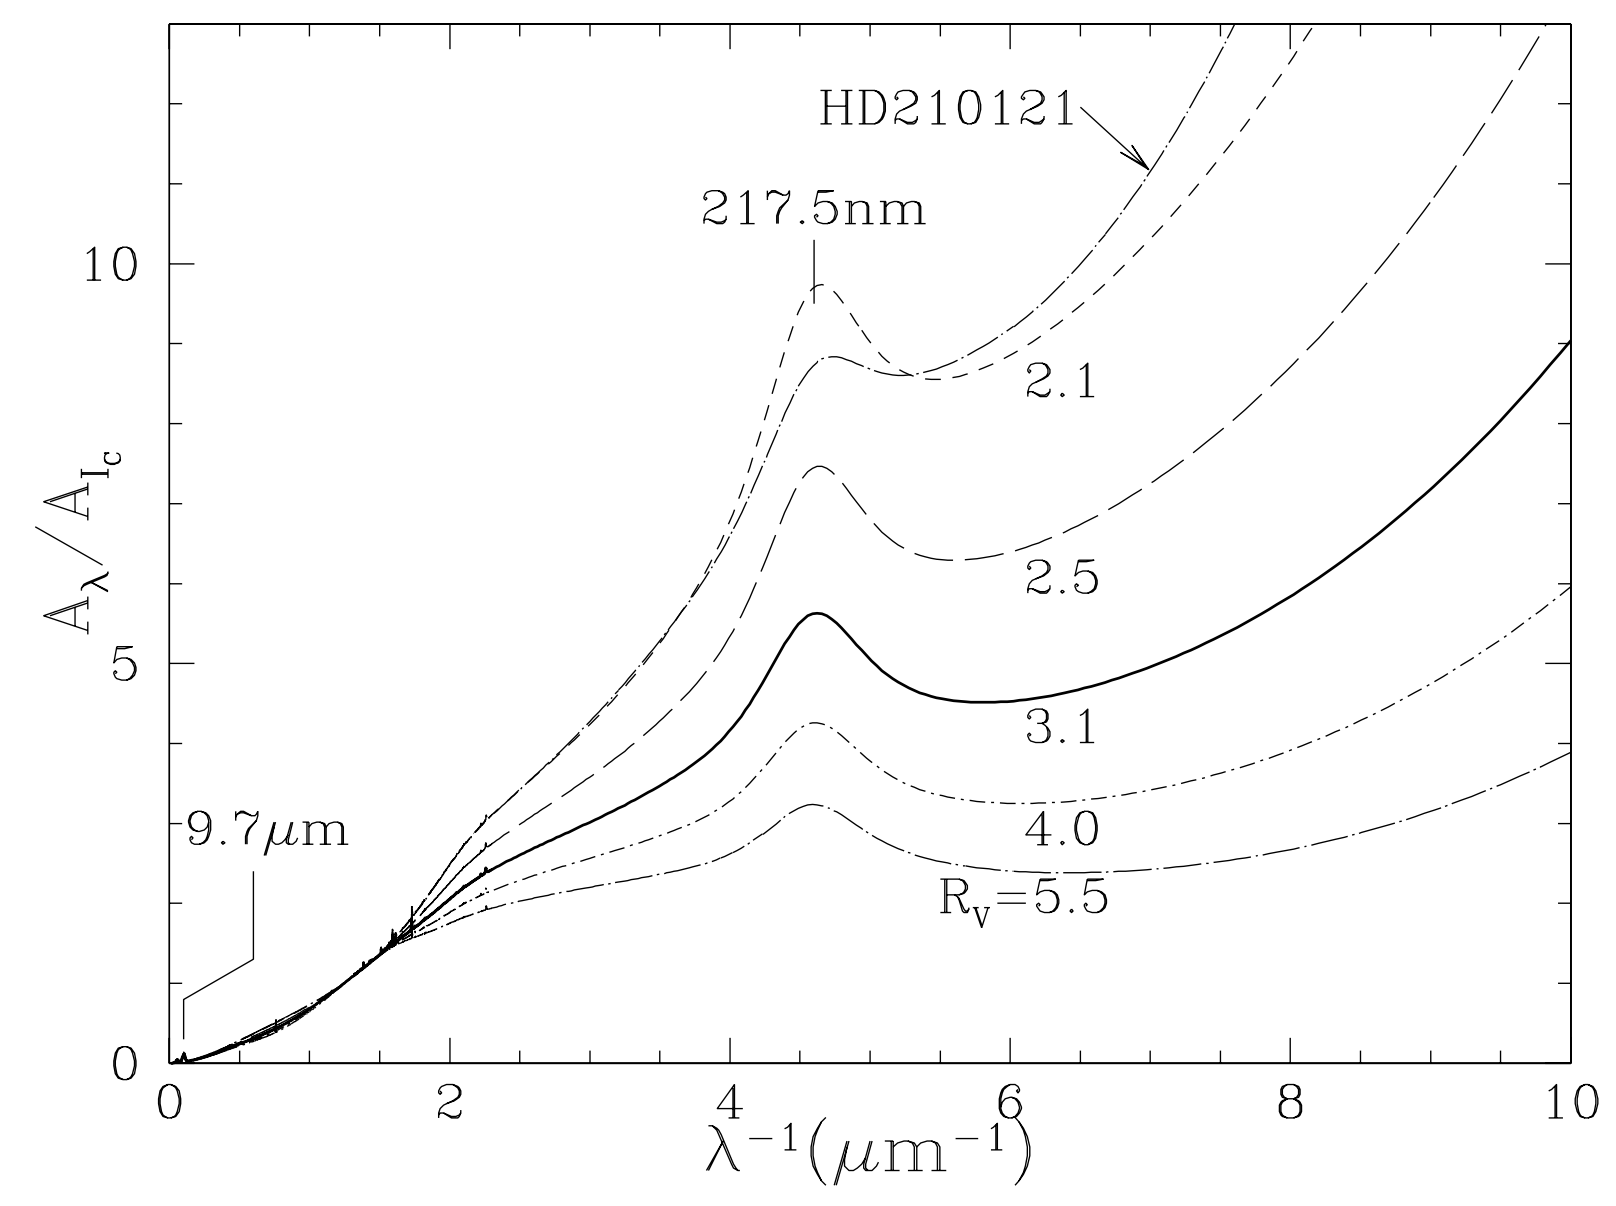
\includegraphics[width=12cm]{figures/ExtinctionCurve.png}
    \caption{\footnotesize{Extinction at wavelength $\lambda$, relative to the extinction in the Cousins I band ($I_C=8020$\AA), as a function of inverse wavelength $\lambda^{-1}$, for Milky Way regions characterized by different values of $R_V\equiv AV/(AB-AV)\equiv AV/E(B−V)$, where $A_B$ is the extinction at $B=0.44\,\mu{\rm m}$, $A_V$ is the extinction at $V=0.55\,\mu{\rm m}$, and the ``reddening'' $E(B−V)\equiv A_B−A_V$. The curves shown are from the one-parameter family of curves $f_1^{\rm CCM}(\lambda)$ parameterized by $R_V$. Also shown is the extinction curve toward the star HD210121 (with $R_V=2.1$), showing that it differs from the CCM extinction curve $f_1^{\rm CCM}$ for $R_V=2.1$. Note the rapid rise in extinction in the vacuum ultraviolet ($\lambda\lesssim0.15\,\mu{\rm m}$) for regions with $R_V\lesssim4$. The normalization per H nucleon is approximately $A_{I_C}/N_H\approx2.9\times10^{-22}\,{\rm mag\,cm^2\,H^{-1}}$. The silicate absorption feature at $9.7\,\mu{\rm m}$ and the diffuse interstellar bands are barely visible. Figure taken from Draine (2011).}}
    \label{fig:extinctioncurve}
\end{figure}

\subsubsection{Additional context}

Dust plays an important role in astrophysics, and the need to characterize and understand dust is increasingly appreciated. Historically, interstellar dust was first recognized for its obscuring effects, and the need to correct observed intensities for attenuation by dust continues today. But with the increasing sensitivity of IR, FIR, and sub-mm telescopes, dust is increasingly important as a diagnostic, with its emission spectrum providing an indicator of physical conditions, and its radiated power bearing witness to populations of obscured stars of which we might otherwise be unaware.

{\noindent}More fundamentally, dust is now understood to play many critical roles in galactic evolution. By sequestering selected elements in the solid grains, and by catalyzing formation of the H2 molecule, dust grains are central to the chemistry of interstellar gas. Photoelectrons from dust grains can dominate the heating of gas in regions where ultraviolet starlight is present, and in dense regions the infrared emission from dust can be an important cooling mechanism. Last, dust grains can be important in interstellar gas dynamics, communicating radiation pressure from starlight to the gas, and coupling the magnetic field to the gas in regions of low fractional ionization.

{\noindent}Barnard was apparently the first to realize that some stars were dimmed by an “absorbing medium.” This was confirmed by Trumpler who showed that the stars in distant open clusters were dimmed by something in addition to the inverse square law, and concluded that interstellar space in the galactic plane contained ``fine cosmic dust particles of various sizes... producing the observed selective absorption.'' Over the succeeding eight decades, we have built on these pioneering studies, but many aspects of interstellar dust (including its chemical composition!) remain uncertain. Let us, therefore, begin by reviewing the different ways in which nature permits us to study interstellar dust.

{\noindent}Trumpler analyzed the interaction of light with interstellar dust, and this remains our most direct way to study interstellar dust. Using stars as ``standard candles,'' we study the ``selective extinction'' (or “reddening'') of starlight by the dust. It is assumed that we know what the spectrum of the star is before reddening by dust takes place; this is usually accomplished by observation of another star with similar spectral features in its atmosphere but with negligible obscuration between us and the star. (This is known as the ``\textbf{pair method}''.)

{\noindent}With the assumption that the extinction ($\equiv$ absorption + scattering) goes to zero at wavelengths $\lambda\rightarrow\infty$, and including observations of the star at sufficiently long wavelength where extinction is negligible, one can determine the attenuation of the starlight by dust as a function of wavelength. Because atomic hydrogen absorbs strongly for $h\nu>13.6\,{\rm eV}$, it is possible to measure the contribution of dust to the attenuation of light only at $h\nu<13.6\,{\rm eV}$, or $\lambda>912$\,\AA. Astronomers customarily characterize the attenuating effects of dust by the ``extinction'' $A_\lambda$ at wavelength $\lambda$. The extinction $A_\lambda$ (measured in ``magnitudes'') is defined by

\begin{align*}
    A_\lambda = 2.5\log_{10}\left(\frac{F_{\lambda,0}}{F_\lambda}\right) ~ [{\rm mag}],
\end{align*}

{\noindent}where $F_\lambda$ is the observed flux from the star, and $F_{\lambda,0}$ is the flux that would have been observed had the only attenuation been from the inverse square law. The extinction measured in magnitudes is proportional to the optical depth:

\begin{align*}
    A_\lambda = 2.5\log(e)\tau_\nu = 1.086\tau_\nu ~ [{\rm mag}].
\end{align*}

{\noindent}A typical ``extinction curve'' (the extinction $A_\lambda$ as a function of wavelength or frequency) is shown in Figure \ref{fig:extinctioncurve}, showing the rapid rise in extinction in the vacuum ultraviolet. Because the extinction increases from red to blue, the light reaching us from stars will be ``reddened'' owing to greater attenuation of the blue light. The detailed wavelength dependence of the extinction (the ``reddening law'') is sensitive to the composition and size distribution of the dust particles. 

{\noindent}Observed extinction curves vary in shape from one line of sight to another. The slope of the extinction at visible wavelengths is characterized by the dimensionless ratio

\begin{align*}
    R_V \equiv \frac{A_V}{A_B-A_V} \equiv \frac{A_V}{E(B-V)} ~ [{\rm dimensionless}],
\end{align*}

{\noindent}where $A_B$ and $A_V$ are the extinctions measured in the $B$ ($4405$\,\AA) and $V$ ($5470$\,\AA) photometric bands, and $E(B-V)\equiv A_B-A_V$ is the ``reddening.''

\begin{table}[t]
    \centering
    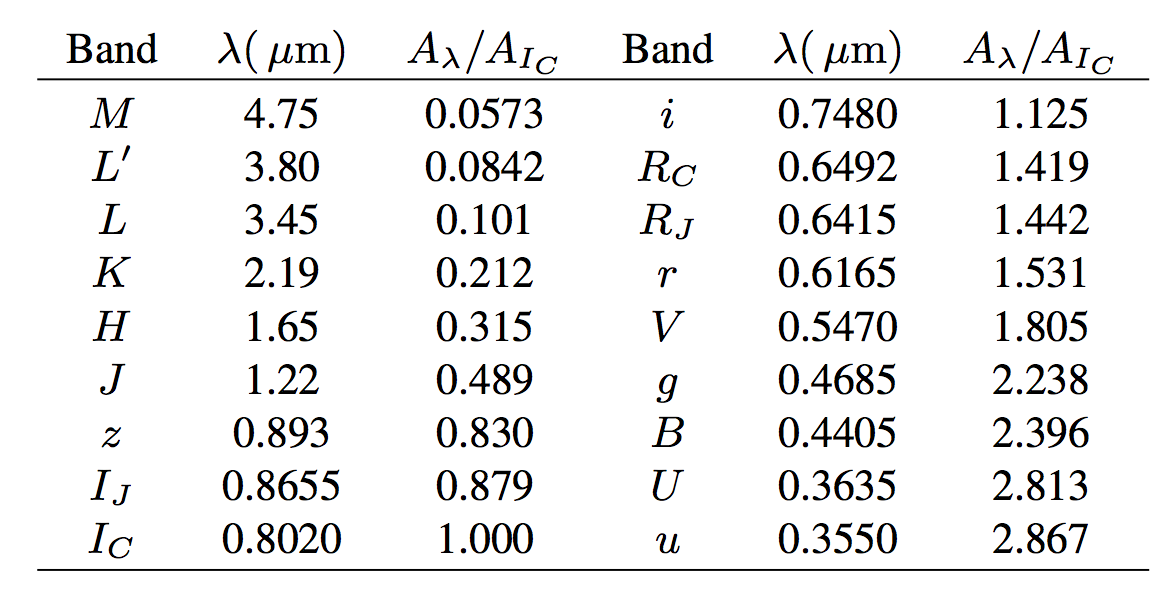
\includegraphics[width=10cm]{figures/ExtinctionTable.png}
    \caption{\footnotesize{Extinction for Standard Photometric Bands for $R_V=3.1$. Figure taken from Draine (2011).}}
    \label{table:extinctiontable}
\end{table}

{\noindent}Sightlines through diffuse gas in the MW have $R_V\approx3.1$ as an average value. The extinction $A_\lambda$, relative to $A_V$, is given in Table \ref{table:extinctiontable} for a number of standard photometric bands for sightlines characterized by $R_V\approx3.1$. The smallest well-determined value is $R_V=2.1$ toward the star HD 210121; the extinction toward HD 201021 is shown in \ref{fig:extinctioncurve}. Sightlines through dense regions tend to have larger values of $R_V$; the sightline toward HD 36982 has $R_V\approx5.7$.

{\noindent}A very useful parametrization of the extinction curve within the MW was provided by Cardelli et al. (1989), who showed that the extinction relative to some reference wavelength $\lambda_{\rm ref}$ can be well-described as a function of $\lambda$ by a fitting function

\begin{align*}
    \frac{A_\lambda}{A_{\rm ref}} \approx f_7^{\rm CCM}(\lambda) ~ [{\rm mag}],
\end{align*}

{\noindent}where $f_7^{\rm CCM}$ has seven adjustable parameters. At wavelengths $3.5\,\mu{\rm m}>\lambda>3030$\,\AA, the function $f_7^{\rm CCM}(\lambda)$ depends only on $\lambda$ and the single parameter $R_V$.

{\noindent}Six parameters are required to describe the UV extinction. Three parameters specify the strength, central wavelength, and width of the $2175$\,\AA\,``bump'' (relative to $A_V$), and three specify the slope and curvature of the continuous extinction underlying the bump and extending to shorter wavelengths. So-called \textbf{CCM extinction curves} are obtained using the function $f_7^{\rm CCM}$ with suitable choices for the $7$ seven fit parameters.

{\noindent}Cardelli et al. (1989) showed that if the single quantity $R_V$ is known, it is possible to estimate the values of the other six parameters so that the optical-UV extinction can be approximated by a one-parameter family of curves:

\begin{align*}
    \frac{A_\lambda}{A_{\rm ref}} \approx f_1^{\rm CCM}(\lambda;R_V) ~ [{\rm mag}],
\end{align*}

{\noindent}It is clear that if the dust grains were large compared to the wavelength, we would be in the ``geometric optics'' limit, and the extinction cross section would be independent of wavelength, with $R_V=\infty$. The tendency for the extinction to rise with decreasing $\lambda$, even at the shortest UV wavelengths where we can measure it, tells us that grains smaller than the wavelength must be making an appreciable contribution to the extinction at all observed wavelengths, down to $\lambda=0.1\,\mu{\rm m}$. ``Small'' means (approximately) that $2\pi a/\lambda\lesssim1$. Thus interstellar dust must include a large population of grains with $a\lesssim0.015\,\mu{\rm m}$.

{\noindent}A number of different quantities are used to characterize the absorption, scattering, and emission of electromagnetic radiation by a (non-rotating) dust grain:

\begin{itemize}
    \item The absorption cross section at wavelength $\lambda$: $C_{\rm abs}(\lambda)$
    \item The scattering cross section: $C_{\rm sca}(\lambda)$
    \item The extinction cross section: $C_{\rm ext}(\lambda) \equiv C_{\rm abs}(\lambda)+C_{\rm sca}(\lambda)$
    \item The albedo:
\end{itemize}

\begin{align*}
    \omega \equiv \frac{C_{\rm sca}(\lambda)}{C_{\rm abs}(\lambda)+C_{\rm sca}(\lambda)} = \frac{C_{\rm sca}(\lambda)}{C_{\rm ext}(\lambda)} ~ [{\rm dimensionless}].
\end{align*}

\begin{itemize}
    \item The differential scattering cross section:
\end{itemize}

\begin{align*}
   \frac{{\rm d}C_{\rm sca}}{{\rm d}\Omega}
\end{align*}

for incident unpolarized light to be scattered by an angle $\theta$. This is related to the dimensionless Muller matrix element $S_{11}$ by

\begin{align*}
   \frac{{\rm d}C_{\rm sca}}{{\rm d}\Omega} \equiv \frac{S_{11}(\theta)}{k^2}
\end{align*}

where $k\equiv2\pi/\lambda$.

\begin{itemize}
    \item The mean value of $\cos\theta$ for scattered light:
\end{itemize}

\begin{align*}
   \langle\cos\theta\rangle = \frac{1}{C_{\rm sca}}\int\limits_0^\pi \cos\theta \frac{{\rm d}C_{\rm sca}}{{\rm d}\Omega} 2\pi\sin\theta{\rm d}\theta ~ [{\rm dimensionless}].
\end{align*}

\begin{itemize}
    \item The radiation pressure cross section:
\end{itemize}

\begin{align*}
   C_{\rm pr}(\lambda) \equiv C_{\rm abs}(\lambda) + (1-\langle\cos\theta\rangle)C_{\rm sca}(\lambda) ~ [{\rm cm^2}].
\end{align*}

\begin{itemize}
    \item The degree of polarization $P(\theta)$ for light scattered through an angle $\theta$ (for incident unpolarized light).
\end{itemize}

{\noindent}For a given direction of incidence relative to a fixed grain, we would obviously need two angles $(\theta,\phi)$ to fully specify the scattering direction. However, for spherical grains, or for an ensemble of randomly oriented grains, the scattering properties can be described as a function of a single scattering angle $\theta$.

{\noindent}In some cases, one wants to consider scattering of polarized light. For this case, it is usual to use the four-element \textbf{Stokes vector} to specify the intensity and state of polarization of radiation propagating in a particular direction. The ability of a grain to scatter radiation with incident Stokes vector $V_{\rm in}$ to outgoing Stokes vector $V_{\rm sca}$ is conveniently specified by a $4\times4$ dimensionless scattering matrix $S_{ij}$, known as the Muller matrix.

{\noindent}It is convenient to normalize the absorption and scattering cross sections $C_{\rm abs}$ and $C_{\rm sca}$ to some area characterizing the grain. In the case of a spherical grain, it is natural to use the grain geometric cross section $\pi a^2$.

{\noindent}For non-spherical grains, some authors choose to normalize using the geometric cross section as seen from the direction of the incident radiation; other authors choose to normalize using the average geometric cross section for random orientations.

{\noindent}Here, we will instead normalize to the geometric cross section of an equal-solid-volume sphere. For a target with solid volume $V$ (V does not include the volume of any voids, if present), we define efficiency factors $Q_{\rm sca}$, $Q_{\rm abs}$ and $Q_{\rm ext} \equiv Q_{\rm abs} + Q_{\rm sca}$ by

\begin{align*}
    Q_{\rm sca} &\equiv \frac{C_{\rm sca}}{\pi a_{\rm eff}^2} ~ [{\rm cm^{-2}}] \\
    Q_{\rm abs} &\equiv \frac{C_{\rm abs}}{\pi a_{\rm eff}^2} ~ [{\rm cm^{-2}}] \\
    a_{\rm eff} &\equiv \left(\frac{3V}{4\pi}\right)^{1/3}  ~ [{\rm \mu m}].
\end{align*}

{\noindent}Here, $a_{\rm eff}$ is the radius of an equal-volume sphere. This is a natural choice, because it relates the scattering and absorption cross sections directly to the actual volume of grain material.

{\noindent}In order to calculate scattering and absorption of electromagnetic waves by targets, we need to characterize the response of the target material to the local oscillating electric and magnetic fields. At submillimeter frequencies and above, real materials have only a negligible response to an applied magnetic field -- this is because the magnetization of materials is the result of aligned electron spins and electron orbital currents, and an electron spin (or orbit) can change direction only on time scales longer than the period for the electron spin (or orbit) to precess in the local (microscopic) magnetic fields within atoms and solids. These fields are at most $B_i\lesssim10\,{\rm kG}$, and the precession frequencies are $\omega_p\approx \mu_BB_i/\hbar\lesssim10^{10}\,{\rm s^{-1}}$, where $\mu_B$ is the \textbf{Bohr magneton} given by the equation

\begin{align*}
    \mu_B \equiv \frac{e\hbar}{2m_ec} ~ [{\rm erg\,G^{-1}}].
\end{align*}

{\noindent}When a weak applied field oscillates at frequencies$\omega\ll10^{10}\,{\rm s^{-1}}$, the magnetization of the material cannot respond. As a result, for frequencies $\nu\geq10\,{\rm GHz}$ we normally set the magnetic permeability $\mu=1$, and consider only the material's response to the oscillating electric field.

{\noindent}The response of material to an applied oscillating electric field $E=E_0e^{-i\omega t}$ is characterized by a complex \textbf{dielectric function} of the permittivity $\epsilon$:

\begin{align*}
    \epsilon(\omega) = \epsilon_1 + i\epsilon_2 ~ [{\rm F\,m^{-1}}].
\end{align*}

{\noindent}The electrical conductivity $\sigma$, if any, can be absorbed within the imaginary part of the dielectric function, with the replacement

\begin{align*}
    \epsilon \rightarrow \frac{4\pi i\sigma}{\omega} ~ [{\rm S\,m^{-1}}].
\end{align*}

{\noindent}The complex \textbf{refractive index} $m(\omega)$ is related to the complex dielectric function by $m=\sqrt{\sigma}$.

\begin{figure}[t!]
    \centering
    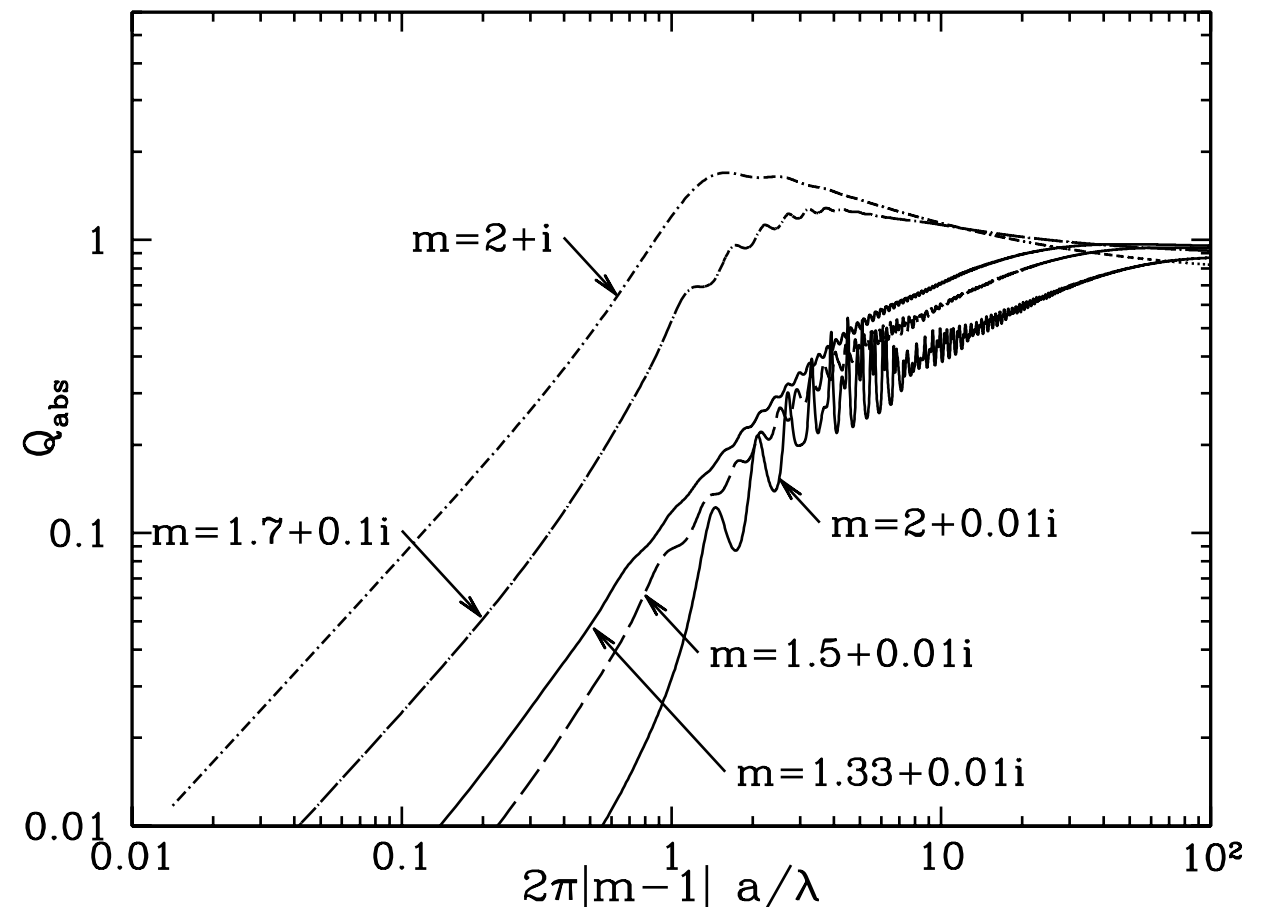
\includegraphics[width=7.5cm]{figures/Qabs.png}
    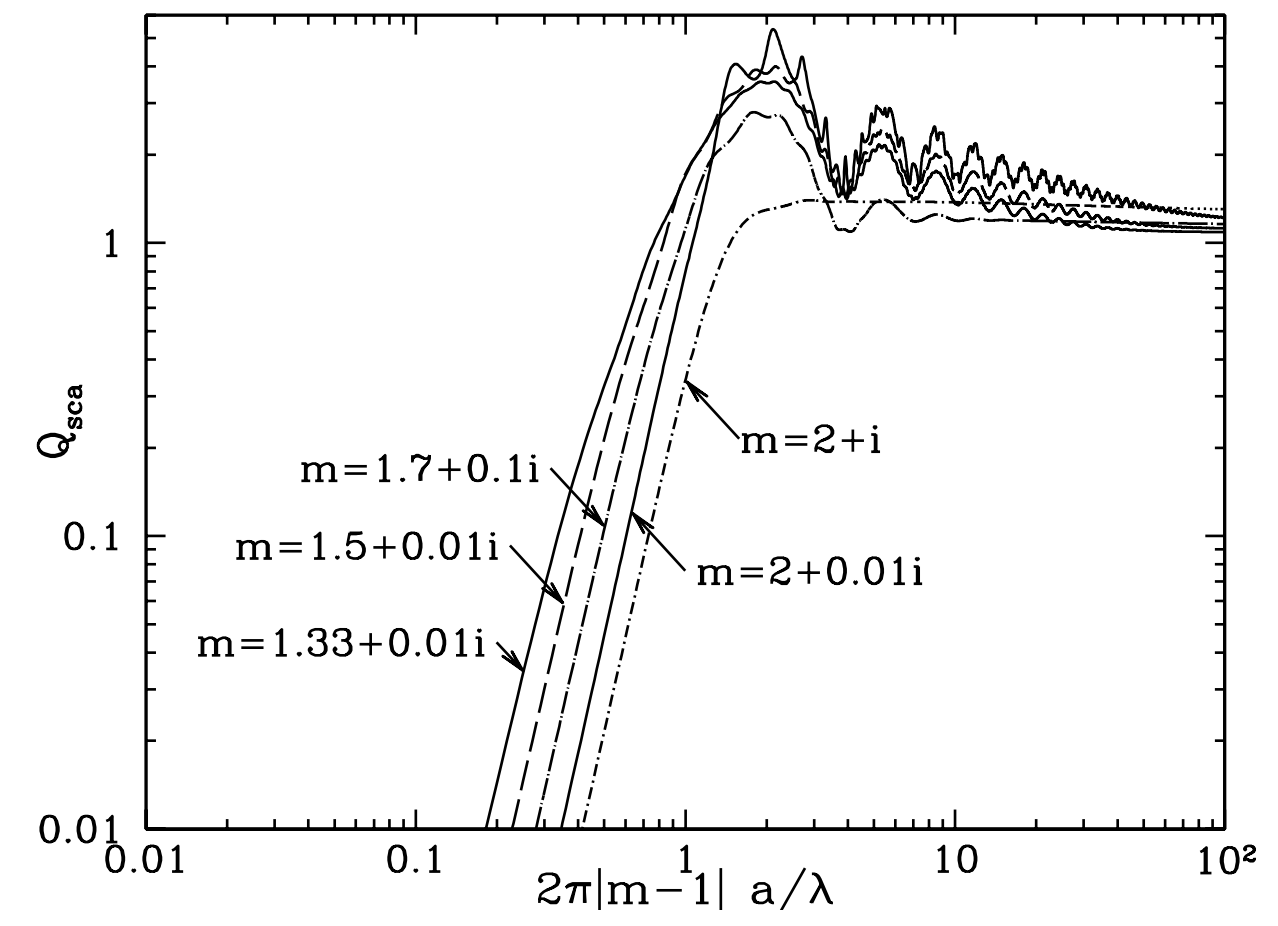
\includegraphics[width=7.5cm]{figures/Qsca.png}
    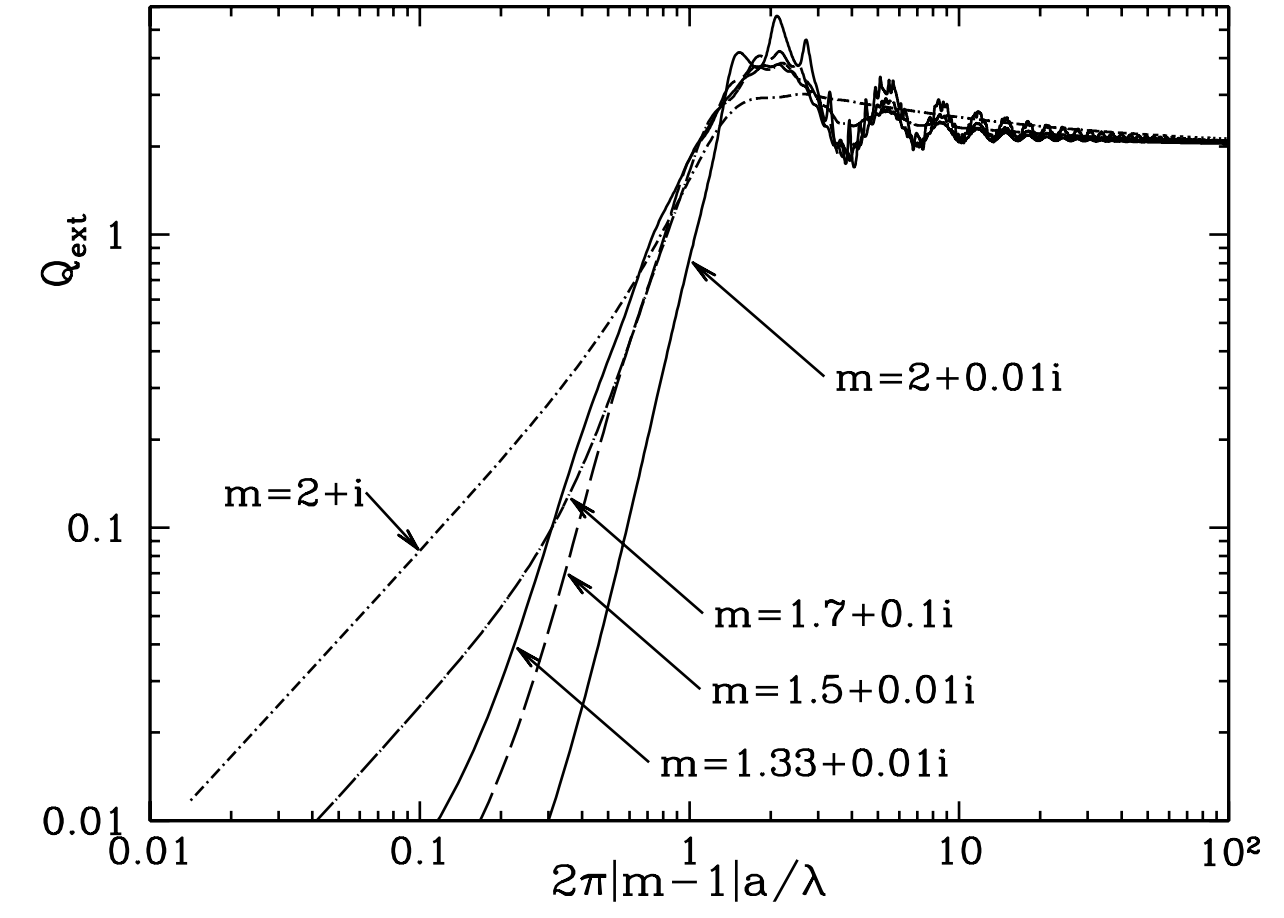
\includegraphics[width=7.5cm]{figures/Qext.png}
    \caption{\footnotesize{\textbf{Top left}: Absorption efficiency factors $Q_{\rm abs}$ for spheres with various refractive indices $m$. \textbf{Top right}: Scattering efficiency factors $Q_{\rm sca}$ for spheres with various refractive indices $m$. \textbf{Bottom}: Extinction efficiency factors $Q_{\rm ext}$ for spheres with various refractive indices $m$. Note that $Q_{\rm ext}\rightarrow2$ for $|m-1|a/\lambda\rightarrow\infty$. Figure taken from Draine (2011).}}
    \label{fig:Q}
\end{figure}

{\noindent}There are two sign conventions for the imaginary part of the dielectric function or refractive index. If we choose to write oscillating quantities $\propto e^{i\vec{k}\cdot\vec{r}}-i\omega t$, then ${\rm Im}(\epsilon)>0$ and ${\rm Im}(m)>0$ for absorbing, dissipative materials, where a propagating wave is attenuated. This is the convention that we will use. In terms of the refractive index, the wave vector

\begin{align*}
    k = m(\omega) \frac{\omega}{c} ~ [{\rm m^{-1}}]
\end{align*}

{\noindent}and, therefore, the electric field

\begin{align*}
    E \propto e^{i(kx-\omega t)} \propto e^{-{\rm Im}(m)\omega x/c} ~ [{\rm N\,C^{-1}}]
\end{align*}

{\noindent}and the power in the wave $(\propto|E|^2)$ decays as ${\rm exp}[−2{\rm Im}(m)\omega x/c]$. Therefore, the attenuation coefficient $\kappa$ and attenuation length $L_{\rm abs} \equiv 1/\kappa$ for the wave are simply

\begin{align*}
    \kappa(\omega) &= 2{\rm Im}(\omega)\frac{\omega}{c} \\
    L_{\rm abs}(\omega) &= \frac{c}{2\omega {\rm Im}(m)} = \frac{\lambda}{4\pi {\rm Im}(m)}
\end{align*}

{\noindent}where $\lambda=2\pi c/\omega$ is the wavelength in vacuo.

{\noindent}We are often interested in situations where the grain is much smaller than the wavelength of the incident EM wave. In this situation, the small grain is subject to an incident applied electric field that is nearly uniform in space. The electric field inside the grain will be proportional to the applied external electric field ${\rm Re}(E)0e^{-i\omega t})$. Averaged over one cycle, the rate per volume at which energy is absorbed within the grain is proportional to $\omega\epsilon 2E_0^2$.

{\noindent}The absorption and scattering cross sections can be written

\begin{align*}
    C_{\rm abs} &= \frac{4\pi\omega}{c} {\rm Im}(\alpha) ~ [{\rm cm^2}] \\
    C_{\rm sca} &= \frac{8\pi}{3}\left(\frac{\omega}{c}\right)^4 |\alpha|^2 ~ [{\rm cm^2}],
\end{align*}

{\noindent}where $\alpha$ is the electric polarizability of the grain: the electric dipole moment of the grain $\vec{\mu}=\alpha\vec{E}$, where $\vec{E}$ is the instantaneous applied electric field. Calculating the polarizability in the limit $\omega a/c\rightarrow0$ becomes a problem in electrostatics.

{\noindent}At optical and UV wavelengths, the dust particles are not necessarily small compared to the wavelength, and the electric dipole approximation is no longer applicable. We must find the solution to Maxwell's equations with an incident plane wave, for an object of specified size and shape, composed of material with a specified dielectric function $\epsilon$ or refractive index $m$.

{\noindent}For the special case of a sphere, an elegant analytic solution was found by Mie (1908) and Debye (1909), and is known as \textbf{Mie theory}. In brief, the EM field inside and outside the sphere can be decomposed into spherical harmonics with appropriate radial functions, with coefficients determined by the need to give an incident plane wave at infinity and to satisfy the continuity conditions at the surface of the sphere. Computer programs to evaluate the Mie theory solution are widely available.

{\noindent}The character of the EM scattering will depend on the dimensionless ratio $a/\lambda$ and on the dimensionless refractive index $m(\omega)$. One relevant parameter will be the phase shift of a wave traveling a distance equal to the grain radius within the grain, expressed in radians. For non-absorptive material, this would be just $2\pi a|m-1|/\lambda$. Figure \ref{fig:Q} shows five examples, where we plot the absorption (top), scattering (middle), and extinction (bottom) efficiency factors against this phase shift.

{\noindent}The details depend on the refractive index $m$, but the general trend is for $Q_{\rm ext}$ to rise to a value $Q_{\rm ext}\approx3-5$ near $|m-1|2\pi a/\lambda\approx2$. For dielectric functions with small imaginary components (i.e., weakly absorbing material, ${\rm Im}(m)\ll1$) $Q_{\rm ext}$ as a function of $a/\lambda$ shows oscillatory behavior due to interference effects, but the oscillations are minimal for strongly absorbing materials $({\rm Im}(m)\gtrsim1])$.

{\noindent}For $(a/\lambda)\rightarrow\infty$, all of these examples have $Q_{\rm ext}\rightarrow2$. This is a general result, sometimes referred to as ``\textbf{the extinction paradox}'': for $x\equiv2\pi a/\lambda\rightarrow\infty$ and $|m-1|x\rightarrow\infty$, the extinction cross section is equal to exactly twice the geometric cross section.

{\noindent}Ray-tracing arguments would lead us to expect the extinction cross section to be equal to the geometric cross section, but diffraction around the target leads to additional small-angle scattering, with the total extinction cross section equal to twice the geometric cross section.

{\noindent}Mie theory is a powerful and robust computational tool with which one can efficiently calculate scattering and absorption by spheres with a wide range of dielectric constants, for $x\equiv2\pi a/\lambda\lesssim10^4$. For $x>10^4$, cancellation in the alternating series leads to round-off errors on machines with 64-bit arithmetic, but for the size distributions that are present in the ISM, scattering by the dust mixture is usually dominated by particles with $x\approx1$, and particles with $x\gg1$ can generally be ignored except at x-ray energies.

{\noindent}However, one thing we know for certain about interstellar grains: the observed polarization of starlight implies that they are not spherical. If the grains are not spherical, how are we to calculate scattering and absorption cross sections? Elegant analytic treatments do exist for spheroids or infinite cylinders, but for more general shapes it is necessary to resort to brute force treatments. One approach that has proven useful is to approximate the actual target (with its particular geometry and dielectric function) by an array of ``point dipoles.'' For a target illuminated by an incident monochromatic EM wave, each of these dipoles is assigned a complex polarizability $\alpha(\omega)$. Each dipole has an instantaneous dipole moment $\vec{\mu}_j=\alpha_j\vec{E}_j$, where $\alpha_j$ is the polarizability tensor for dipole $j$, and $\vec{E}_j$ is the electric field at location $j$ due to the incident wave plus all of the other dipoles. This method is known as the \textbf{discrete dipole approximation} (DDA) or coupled dipole approximation.

{\noindent}DDA calculations are CPU-intensive, but many problems of practical interest can be handled by a desktop computer. For example, the DDA has been used to study absorption and scattering by graphite particles and by random agglomerates.

{\noindent}Figure 22.4 shows the real and imaginary components of the dielectric function for ${\rm Mg\,Fe\,Si\,O_4}$. In the optical and UV, normal solids have refractive indices $|m-1|\gtrsim0.3$. At x-ray energies, however, $|m-1|\ll1$, and the character of the scattering changes considerably. The wavelength $\lambda=0.00124\,({\rm keV}/h\nu)\,\mu{\rm m}$ is small compared to the sizes $a\approx0.2\,\mu{\rm m}$ of the particles containing most of the grain mass. The result is that the x-ray scattering is very strongly peaked in the forward direction, with a characteristic scattering angle

\begin{align*}
    \theta \approx \frac{\lambda}{\pi a} \approx 800'' \left(\frac{{\rm keV}}{h\nu}\right) \left(\frac{0.1\,\mu{\rm m}}{a}\right) ~ [{\rm rad}].
\end{align*}

\begin{figure}[t]
    \centering
    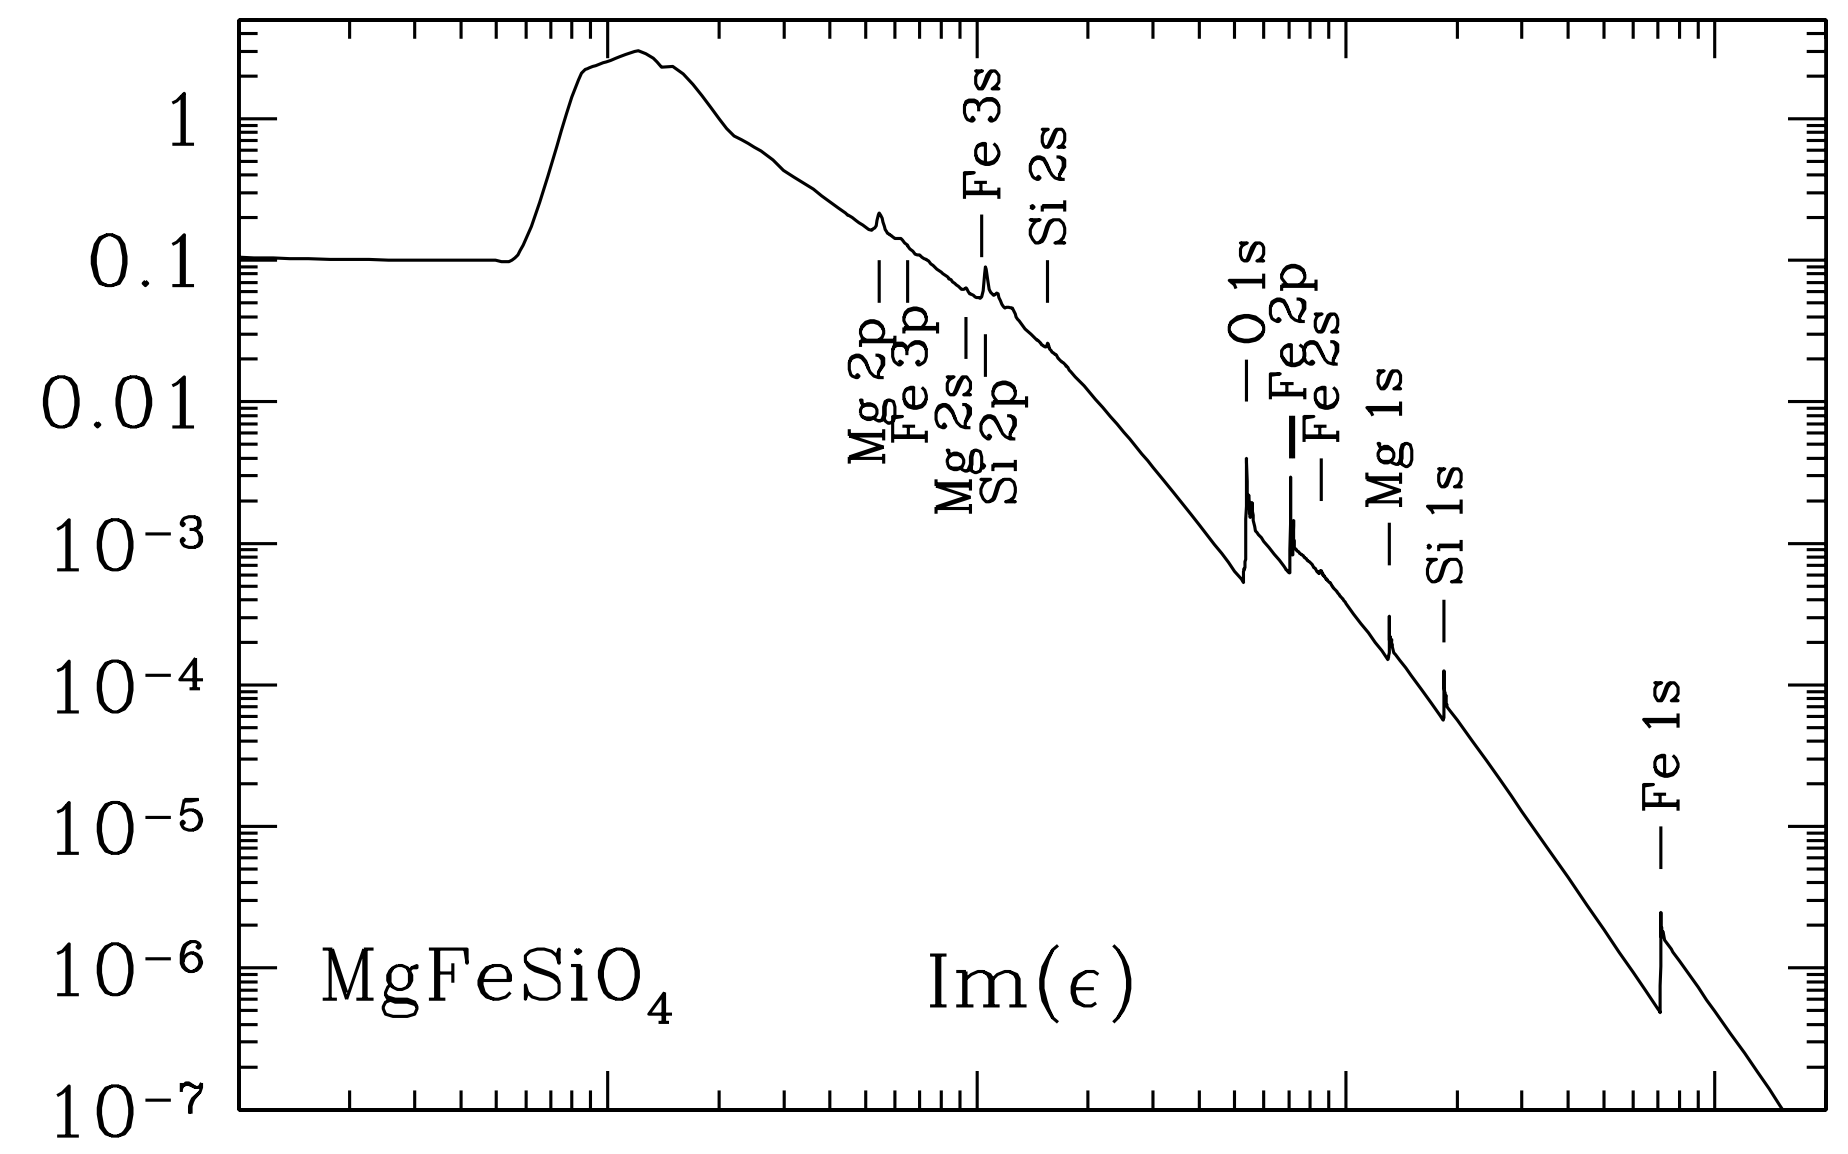
\includegraphics[width=7.5cm]{figures/MgFeSiO4_top.png} 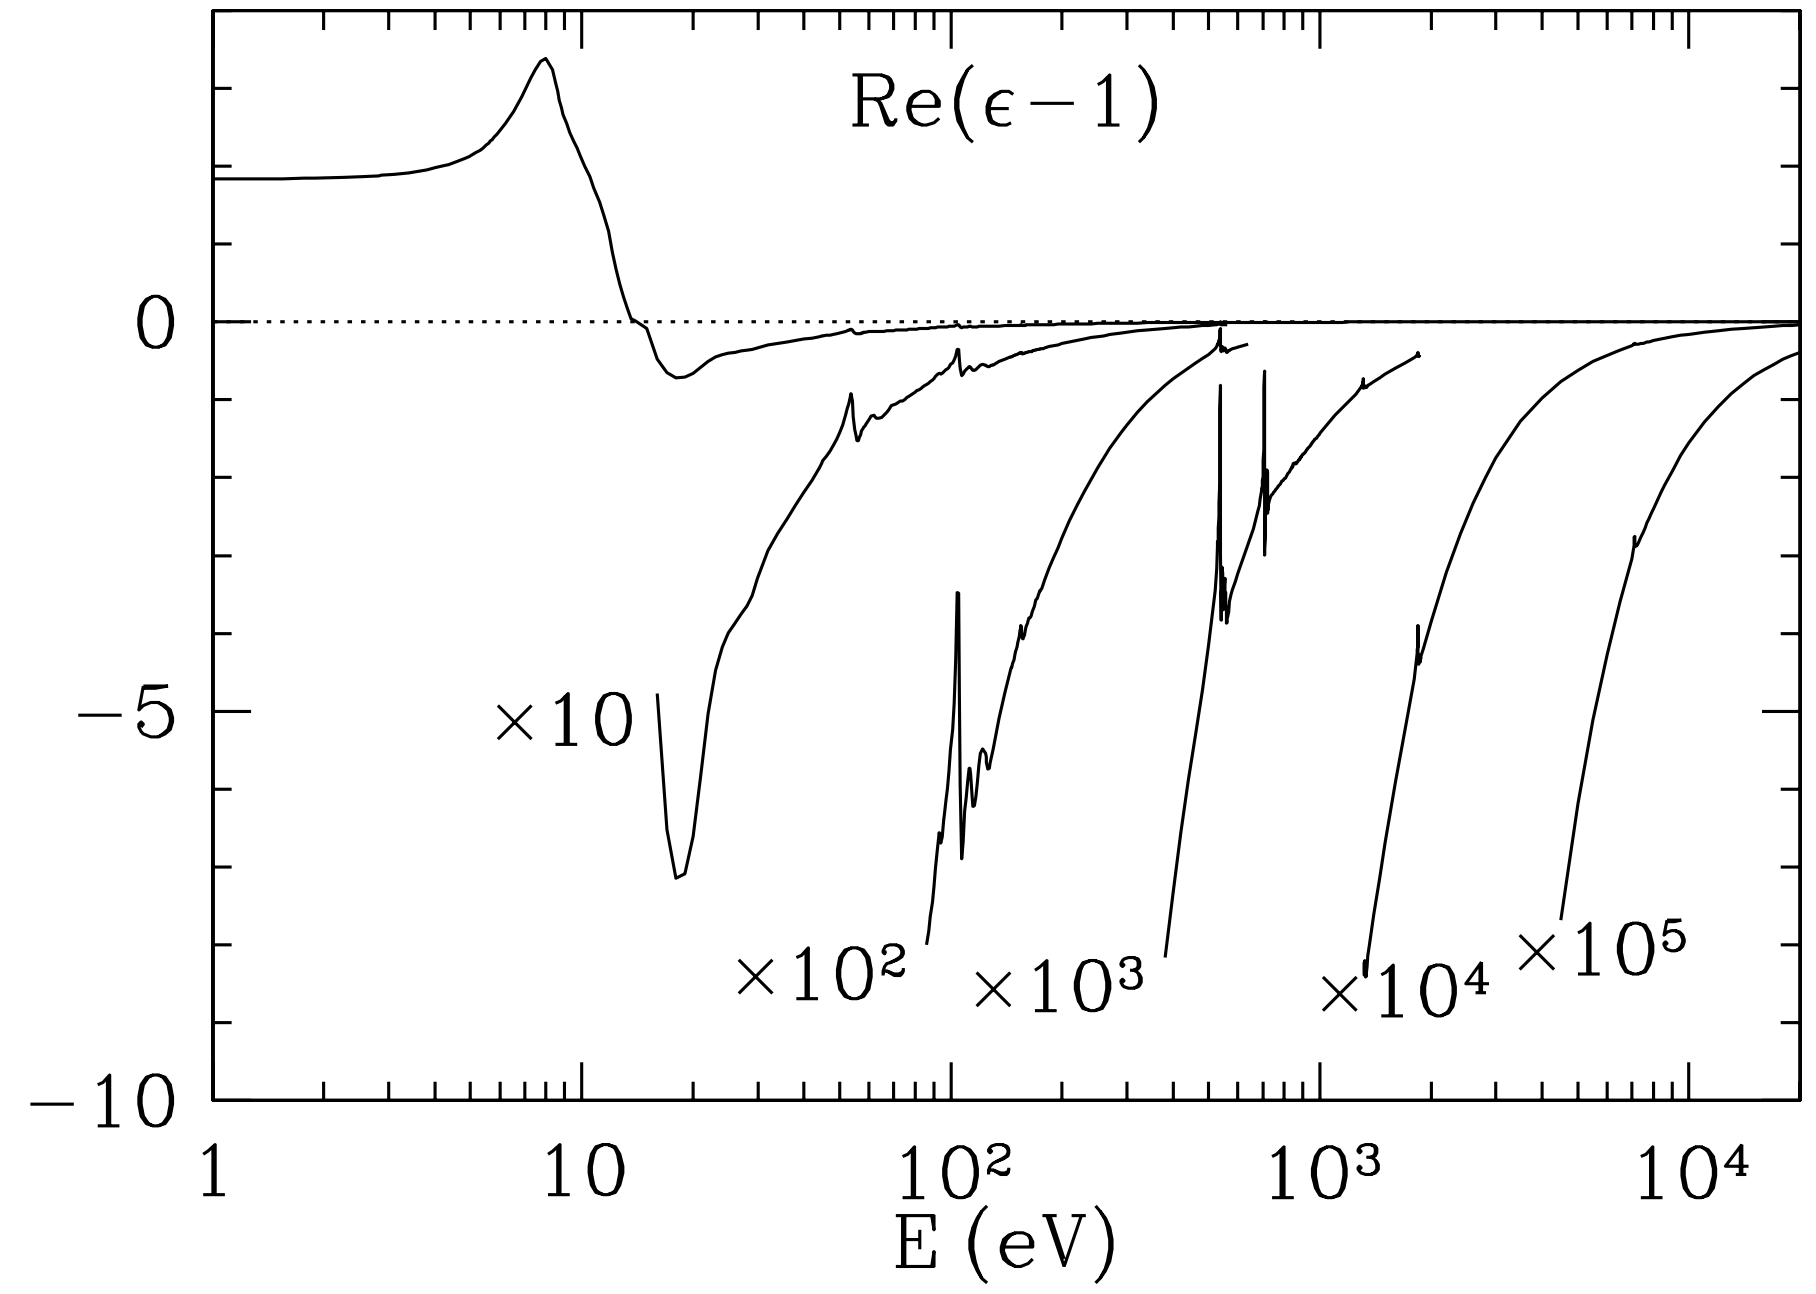
\includegraphics[width=7.5cm]{figures/MgFeSiO4_bottom.png}
    \caption{\footnotesize{Dielectric function $\epsilon$ for ${\rm Mg\,Fe\,Si\,O_4}$ material. Various absorption edges are labelled in the plot of ${\rm Im}(\epsilon)$. This dielectric function, and its continuation at lower energies, will be referred to as ``\textbf{astrosilicate}''. From Draine (2003b), reproduced by permission of the AAS. Figure taken from Draine (2011).}}
    \label{fig:MgFeSiO4}
\end{figure}

{\noindent}Above we have discussed calculational methods for various regimes. We can now calculate scattering and absorption cross sections for micron- or submicron-sized grains from x-ray to sub-mm wavelengths. Figure \ref{fig:Qextgrainsizes} shows the extinction efficiency $Q_{\rm ext}$ calculated for grains of amorphous silicate (``astrosilicate'') from the x-ray to the submm, for four different sizes. There are several noteworthy features:

\begin{itemize}
    \item $Q_{\rm ext}$ shows sharp discontinuities at x-ray absorption edges. The amorphous silicate material is assumed to have composition ${\rm Mg\,Fe\,Si\,O_4}$. Two conspicuous edges are the ${\rm Fe\,K}$ edge at $1.75$\AA~($7.1\,{\rm keV}$) and the ${\rm O\,K}$ edge at $23$\AA~($528\,{\rm eV}$). Note that the appearance of these edges depends on grain size. As the grains become larger, scattering makes an appreciable contribution to $Q_{\rm ext}$, and the long-wavelength side of the ${\rm O\,K}$ edge is ``filled in'' by scattering.
    \item $a=1\,\mu{\rm m}$ grains are, in effect, optically thick (with $Q_{\rm ext}\approx2$) for $0.001\lesssim\lambda\lesssim 2\,\mu{\rm m}$; for $\lambda < 10^{-3}\,\mu{\rm m}$ ($h\nu>1.24\,{\rm keV}$), the absorption length exceeds the grain diameter, and for $\lambda>2\,\mu{\rm m}$, the grain is smaller than the wavelength. Similarly, the $a=10\,\mu{\rm m}$ grain is optically thick for $10^{-4}\,\mu{\rm m} \lesssim\lambda\lesssim 10\,\mu{\rm m}$.
    \item The silicate absorption features at $9.7$ and $18\,\mu{\rm m}$ are prominent absorption features for the $a=0.01,\,0.1,\,1\,\mu{\rm m}$ cases shown, but are suppressed in the $a=10\,\mu{\rm m}$ example, because the grain is, in effect, optically thick at wavelengths on either side of the silicate features.
\end{itemize}

\begin{figure}[t]
    \centering
    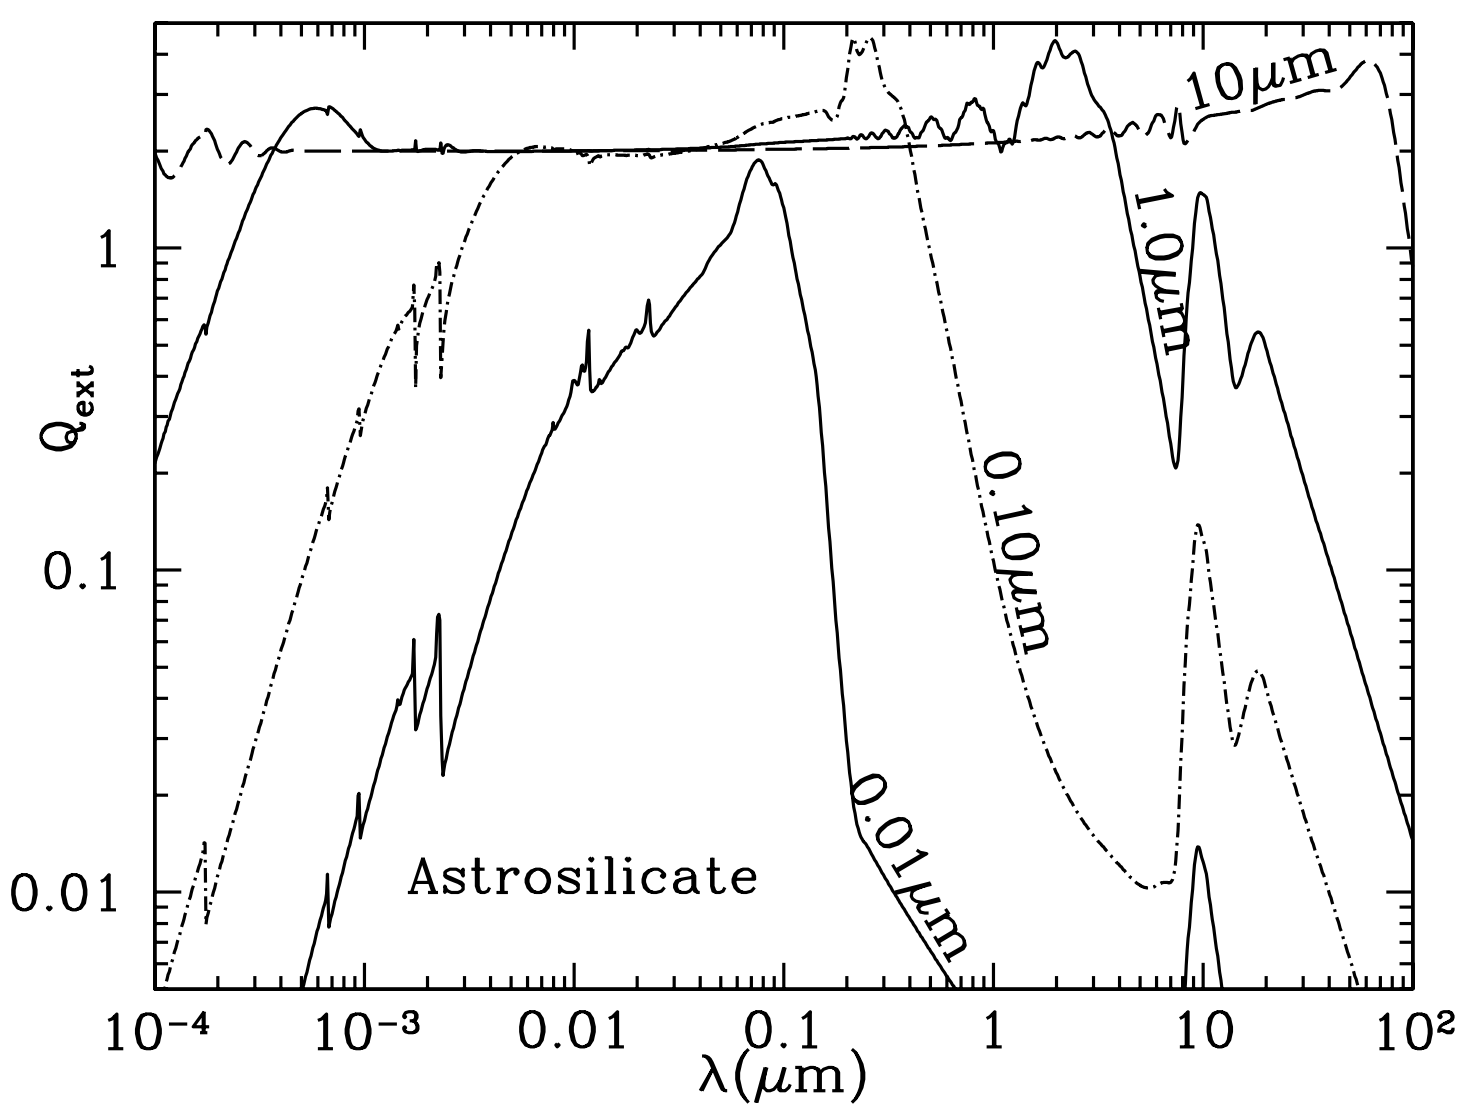
\includegraphics[width=10cm]{figures/Qext_grainsizes.png}
    \caption{\footnotesize{$Q_{\rm ext}\equiv C_{\rm ext}/\pi a2$ for $a=0.01,0.1,1,~{\rm and}~10\,\mu{\rm m}$ amorphous silicate spheres, for wavelengths ranging from $\lambda=10^{-4}\,\mu{\rm m}=1$\AA\, $(h\nu=12.4\,{\rm keV}$) to $\lambda=10^3\,\mu{\rm m}=1\,{\rm mm}$. At short wavelengths, the $a=0.01$ and $0.10\,\mu{\rm m}$ grains show discontinuities in $Q_{\rm ext}$ at x-ray absorption edges. In the IR, the $a=0.01,0.1,1\,\mu{\rm m}$ grains show prominent silicate absorption features at $9.7$ and $18\,\mu{\rm m}$, but these features are suppressed when $a=10\,\mu{\rm m}$. Figure taken from Draine (2011).}}
    \label{fig:Qextgrainsizes}
\end{figure}

\begin{figure}[b]
    \centering
    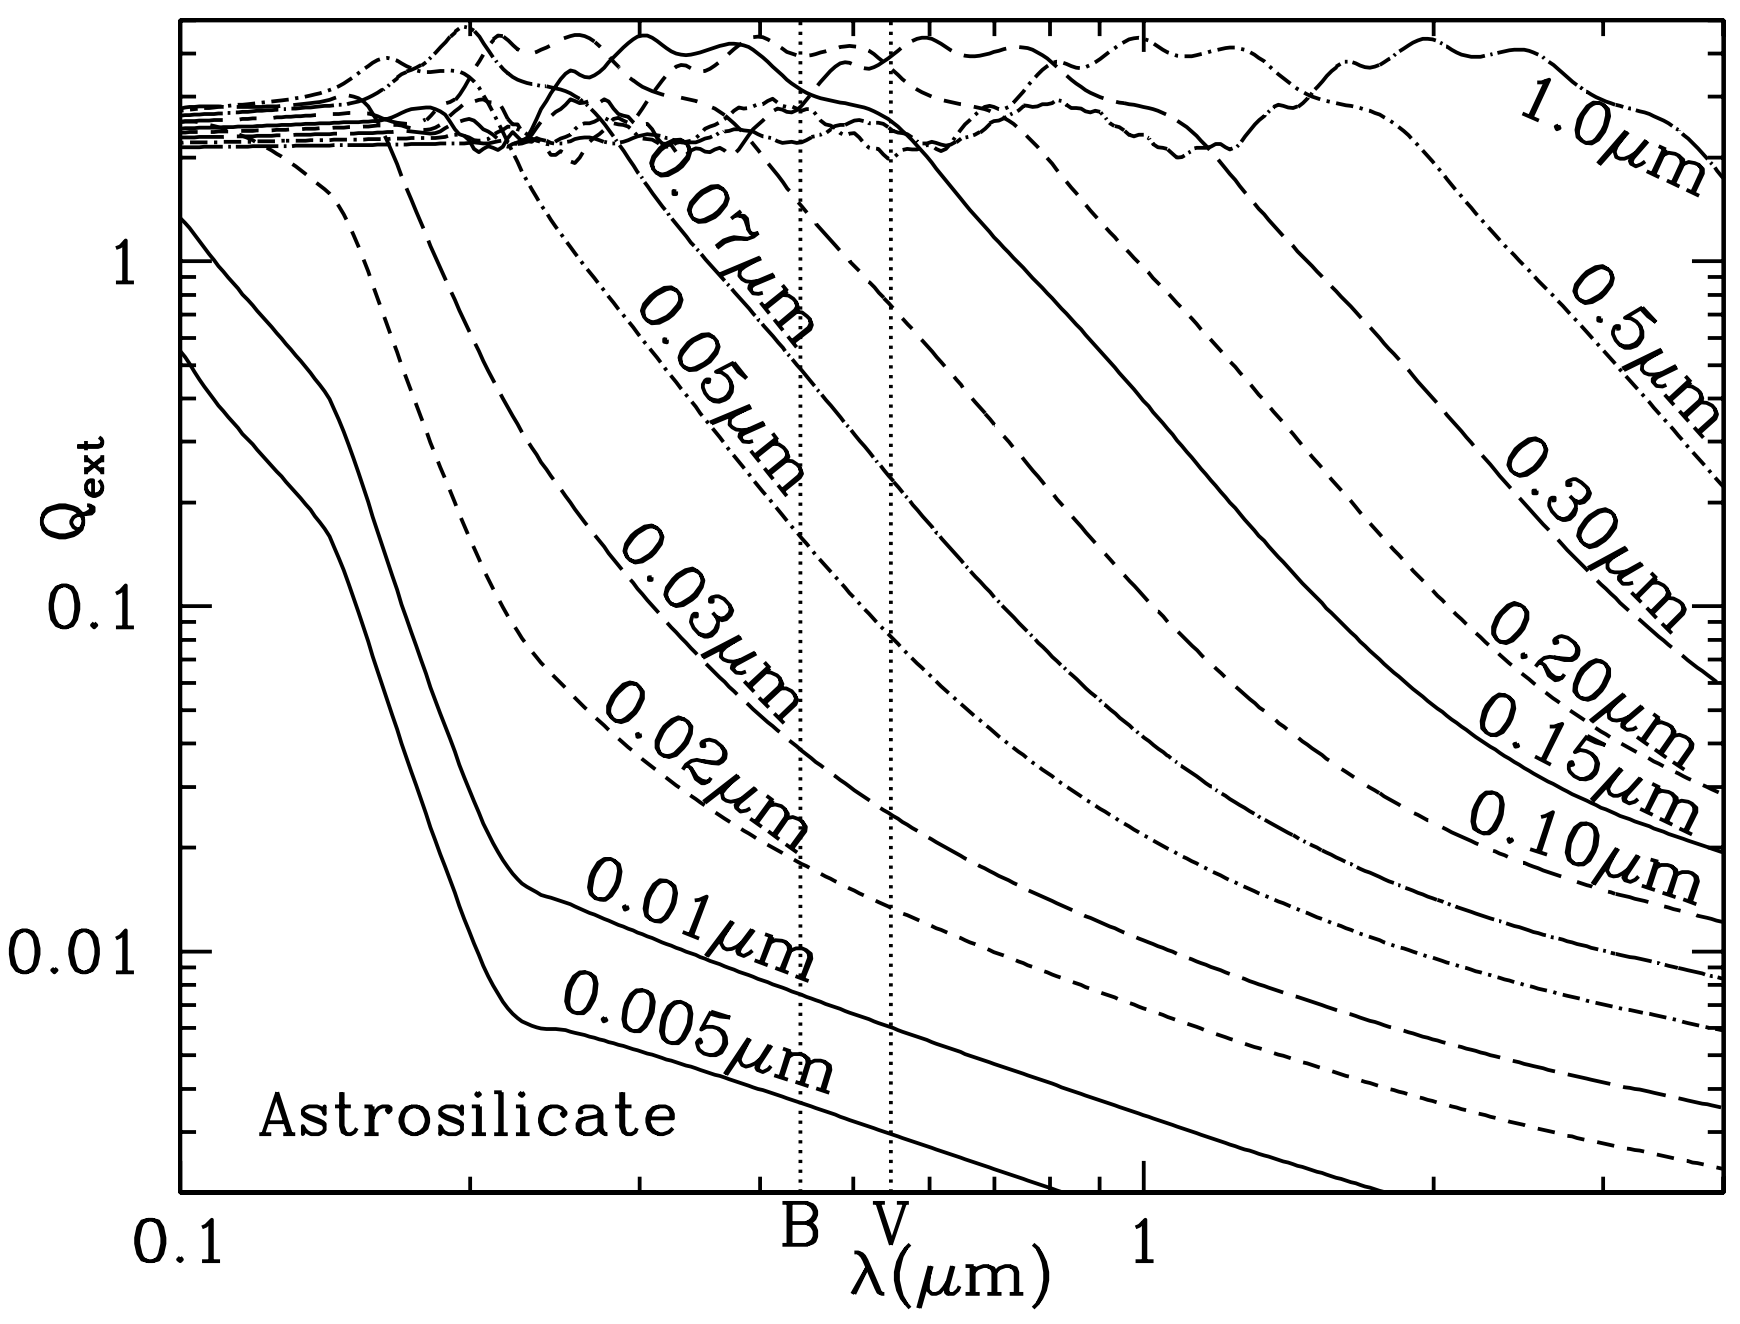
\includegraphics[width=7.5cm]{figures/Qext_BV_top.png}
    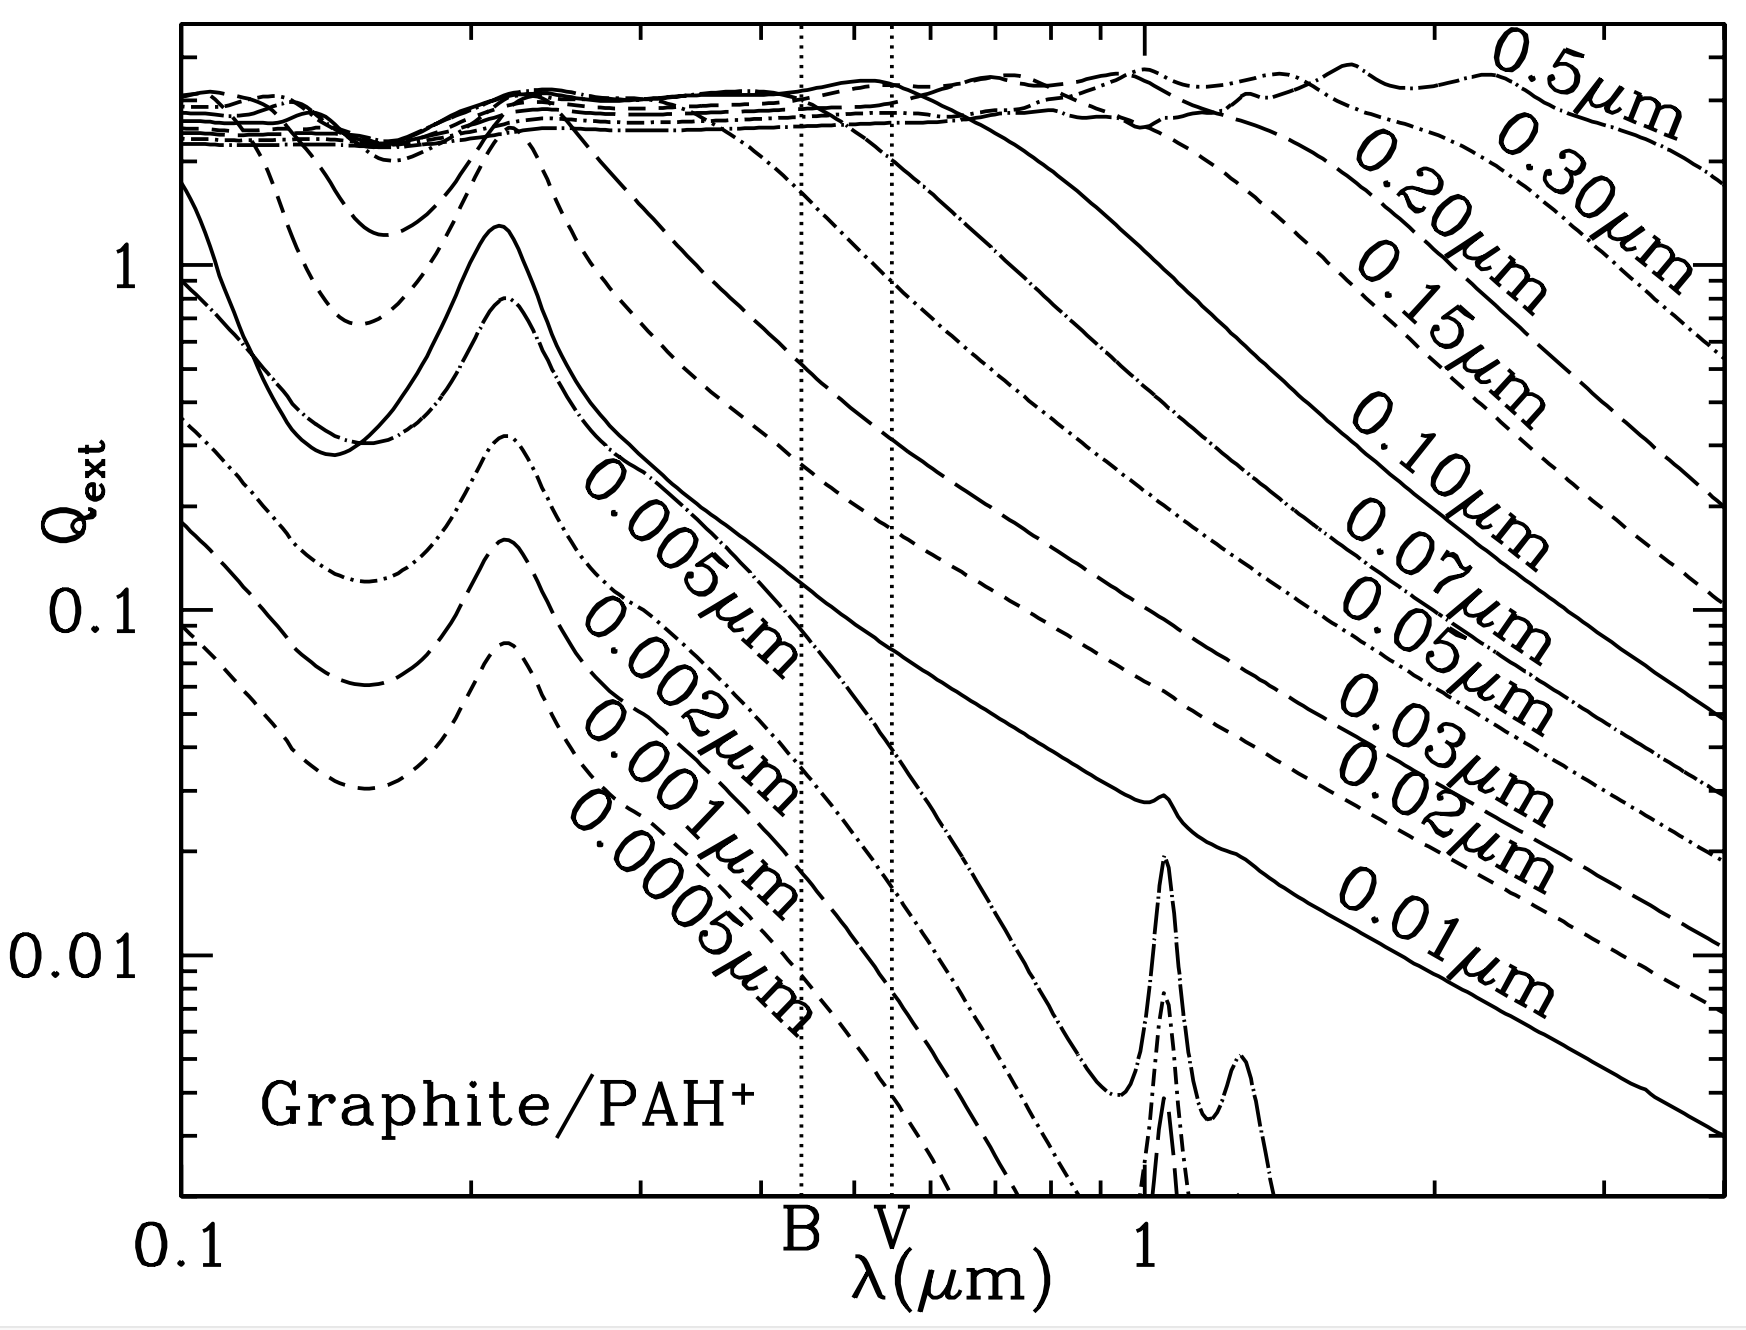
\includegraphics[width=7.5cm]{figures/Qext_BV_bottom.png}
    \caption{\footnotesize{$Q_{\rm ext}$ for astrosilicate spheres (left) and carbonaceous spheres (right) for wavelengths ranging from $\lambda=0.1,\mu{\rm m}$ to $\lambda=4,\mu{\rm m}$. The locations of the $B$ ($4405$\AA) and $V$ ($5470$\AA) bands are shown. Curves are labeled by radius $a$. Figure taken from Draine (2011).}}
    \label{fig:QextBV}
\end{figure}

{\noindent}Figure \ref{fig:QextBV} shows the behavior of $Q_{\rm ext}$ for wavelengths running from the vacuum UV into the infrared. The upper panel shows the extinction efficiency factors $Q_{\rm ext}$ for spheres with the ``astrosilicate'' dielectric function. For the wavelength range shown here, there are no spectral features, although small particles do show a rise in extinction for $\lambda\lesssim0.2,\mu{\rm m}$ due to the onset of ultraviolet absorption in silicates. Scattering becomes important for $\lambda\lesssim2\pi a$ (i.e., $x=2\pi a/\lambda\gtrsim1$), and $Q_{\rm ext}\gtrsim2$ for $\lambda\lesssim4a$.

{\noindent}For the adopted optical constants, the small ($a\lesssim0.02\,\mu{\rm m}$) carbonaceous particles show a strong absorption feature near $2175$\AA, closely matching the observed interstellar feature near this wavelength. However, the theoretically-calculated feature broadens as the grain size increases to $0.03\,\mu{\rm m}$, and disappears for larger grains because the grain becomes optically thick not only at the wavelength of the resonance, but also at wavelengths above and below the resonance.

{\noindent}As discussed earlier, interstellar extinction curves are often characterized by $R_V\equiv A_V/(A_B-A_V)$, and it is of interest to see what value of RV would apply to the extinction produced by grains of a single size and composition. Because $R_V$ is singular when $A_B=A_V$, it is preferable to instead consider $1/R_V \equiv (A_B-A_V)/A_V$, which is proportional to the slope of the extinction curve between $V$ and $B$. Figure \ref{fig:RVinv} shows $1/R_V$ versus grain radius for carbonaceous grains and astrosilicate grains. For very small grains, scattering is negligible compared to absorption, and the value of $R_V$ in the limit $a\rightarrow0$ depends on the wavelength dependence of the optical constants-- hence the very different limiting values for PAHs and astrosilicates. As the grain radius is increased, scattering begins to contribute significantly to the extinction, but we see that neither the silicate nor carbonaceous particles ever reach the value of $1/R_V=1/0.726$ appropriate to Rayleigh scattering by particles with a polarizability that is wavelength independent. This is because, for our assumed dielectric functions, when the particles are small enough to be in the Rayleigh limit, absorption makes an important contribution to the extinction.

\begin{figure}[t]
    \centering
    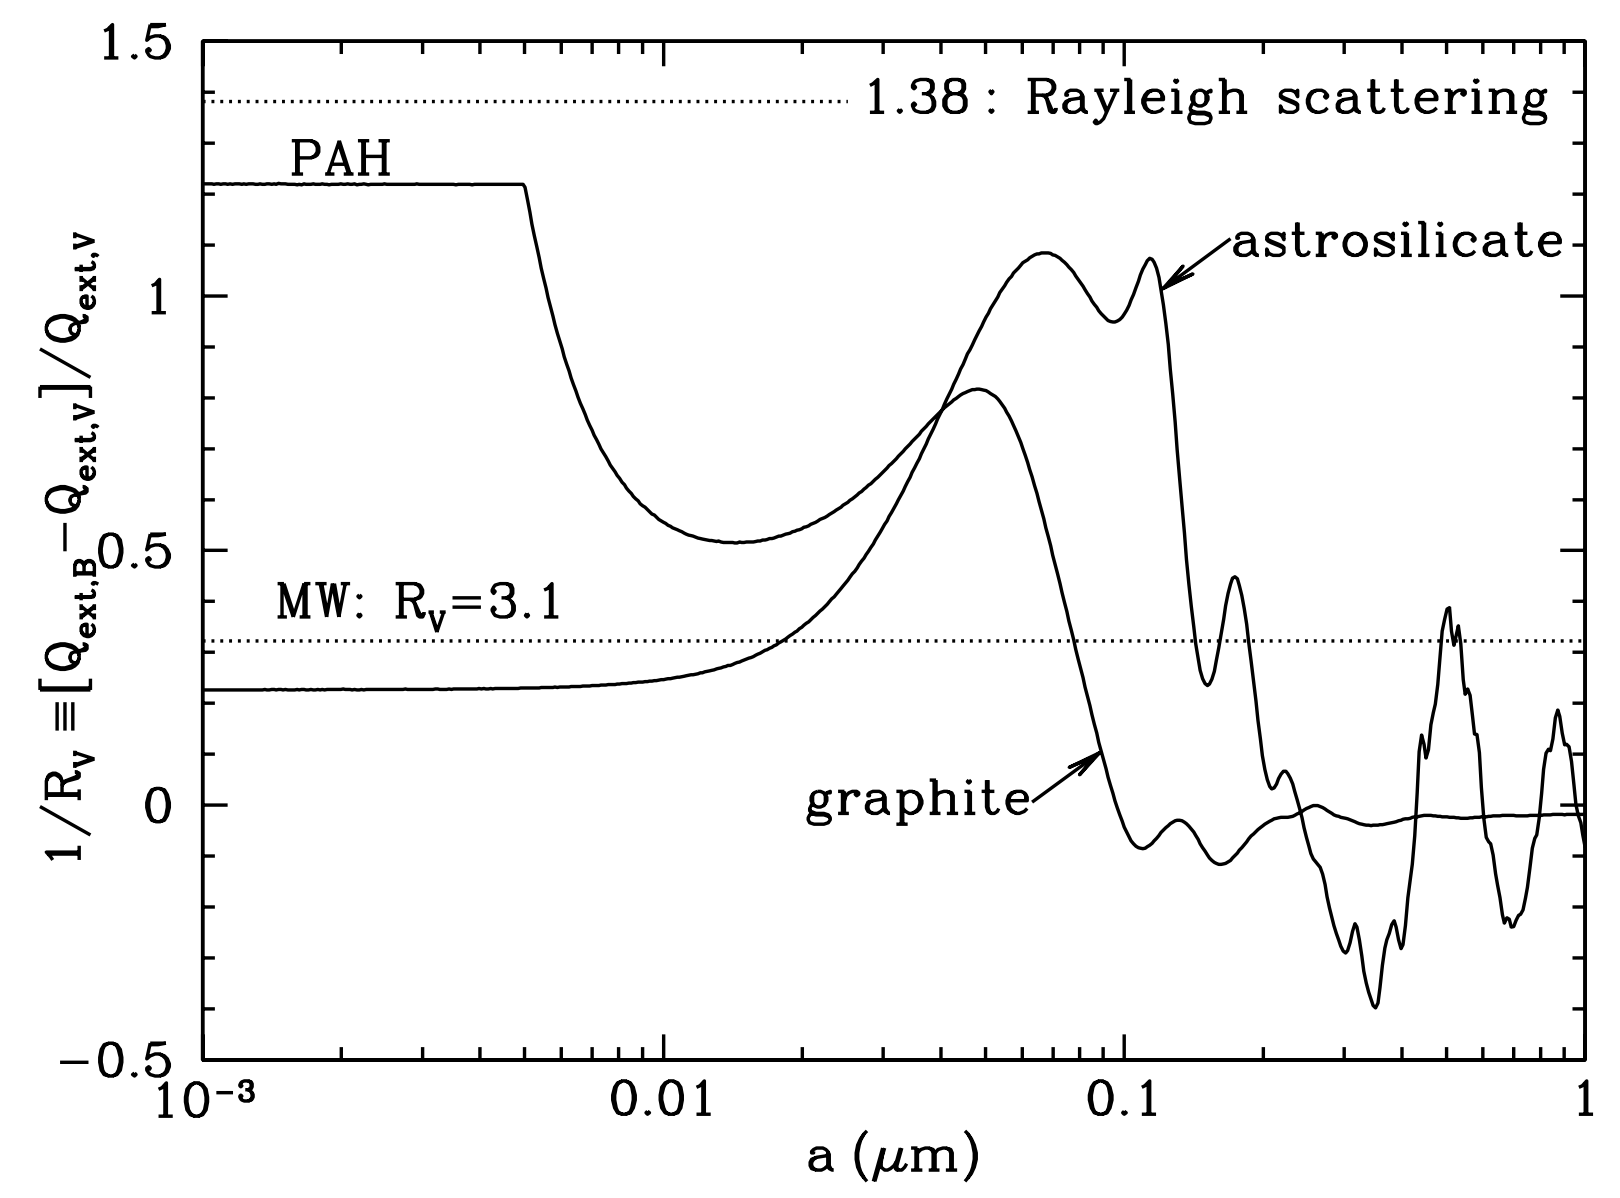
\includegraphics[width=10cm]{figures/RV_inv.png}
    \caption{\footnotesize{$1/R_V \equiv (C_{\rm ext}(B) - C_{\rm ext}(V))/C_{\rm ext}(V)$ as a function of radius a for astrosilicate and carbonaceous spheres ($B=0.44\,\mu{\rm m},\,V=0.55\,\mu{\rm m}$). The carbonaceous spheres are assumed to be graphitic for $a>0.01\,\mu{\rm m}$, and PAHs for $a<0.005\,\mu{\rm m}$, with a continuous transition between $0.005$ and $0.01\,\mu{\rm m}$. For $a\lesssim0.02\,\mu{\rm m}$, scattering is unimportant, and $R_V$ is determined by the absorptive properties of the grain material. For $a\gtrsim0.12\,\mu{\rm m}$, scattering resonances move through the wavelength range between $B$ and $V$, and $1/R_V$ has oscillatory behavior. The dust in the diffuse ISM is observed to have $R_V\approx3.1$, shown by the dotted line. $R_V\approx3.1$ for $a\approx0.08\,\mu{\rm m}$ or $0.14\,\mu{\rm m}$ for graphitic and astrosilicate grains, respectively. Figure taken from Draine (2011).}}
    \label{fig:RVinv}
\end{figure}

{\noindent}$R_V\approx3.1$ is attained by graphitic grains for $a\approx0.08\,\mu{\rm m}$, and by astrosilicate grains for $\approx0.15\,\mu{\rm m}$. Although a broad size distribution is required to match the full extinction curve, grain models that reproduce the observed extinction should have the extinction in the visible dominated by grains with $a\approx0.1\,\mu{\rm m}$.


\subsubsection{Follow-up Questions}

\begin{itemize}
    \item What happens at shorter wavelengths, like gamma rays?
\end{itemize}

% --------------------------------------------------------------
%               10. 
% --------------------------------------------------------------

\newpage
\subsection{Question 10}

What is dynamical friction? Explain how this operates in the merger of a small galaxy into a large one.

\subsubsection{Short answer}

Answer.

\subsubsection{Additional context}

Additional context.

% --------------------------------------------------------------
%               11. 
% --------------------------------------------------------------

\newpage
\subsection{Question 11}

Sketch the SED, from the radio to Gamma, of a spiral galaxy like the Milky Way. Describe the source and radiative mechanism of each feature.

\subsubsection{Short answer}

\begin{figure}[h]
    \centering
    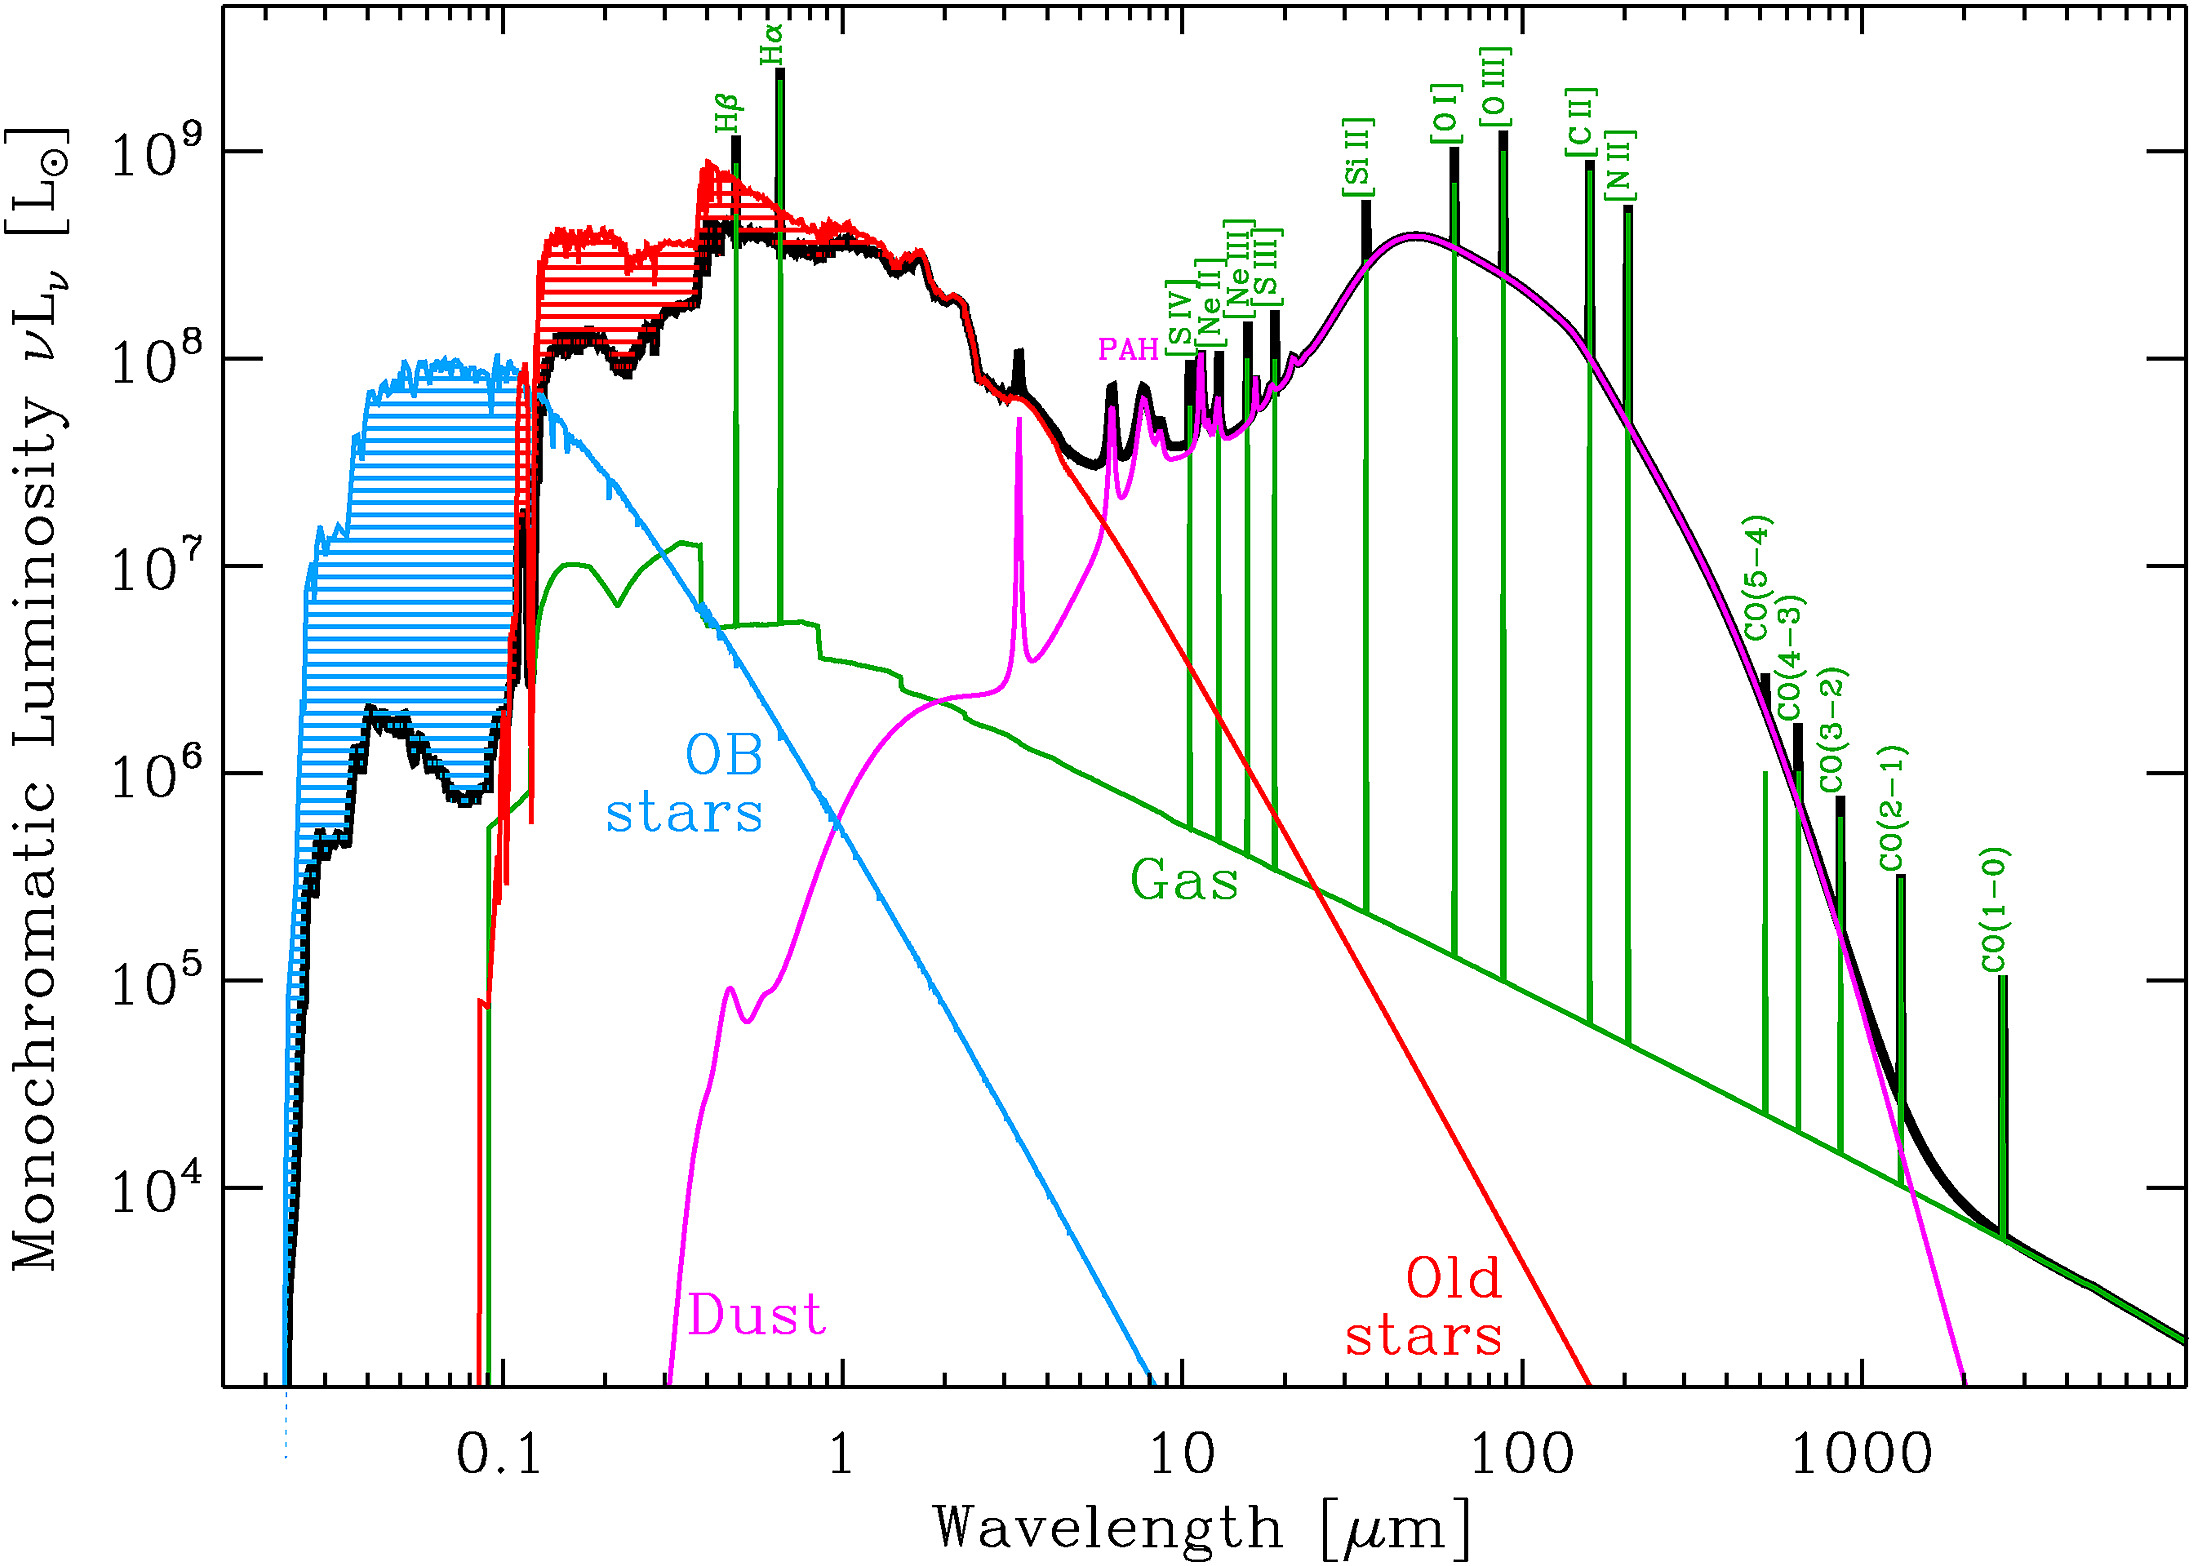
\includegraphics[width=14cm]{figures/GalaxySED.jpg}
    \caption{\footnotesize{Typical SED of a star forming galaxy. It is based on the model of NGC 1569 by Galliano et al. (2008), with the addition of a typical gas contribution, modelled with Cloudy (Ferland et al., 2013). Only the most widely observed gas lines have been shown. The hatched areas in the stellar spectra represent the fraction of light that has been absorbed by the ISM (mainly the dust). This absorbed light is re-emitted by the dust component. Figure taken from Galliano (2017).}}
    \label{fig:galaxySED}
\end{figure}

{\noindent}The spectral energy distribution (SED; see Figure \ref{fig:galaxySED}) of a typical galaxy is dominated by several processes:

\begin{itemize}
    \item \textbf{Stars.} Young OB stars are strong UV emitters, while older stellar populations dominate the visible/near-IR range. The weights of these two main components depend on the SF history of the galaxy. The fraction of light absorbed by dust is represented by the hatched area on Figure \ref{fig:galaxySED}.
    \item \textbf{Gas.} Atomic and molecular lines are numerous, but the gas also emits continuum radiation (Figure \ref{fig:galaxySED}): (i) thermal continuum in the form of free-bound and free-free emission; and (ii) non-thermal continuum, mainly synchrotron.
    \item \textbf{Dust.} Dust radiates thermally over the whole IR domain. Several molecular and solid state features can be seen, mainly in the mid-IR. Figure \ref{fig:dustpah} represents the aromatic feature emission believed to be carried by polycyclic aromatic hydrocarbons (PAH). The whole power emitted by the dust equals the absorbed stellar power (hatched areas of Figure \ref{fig:galaxySED}).
\end{itemize}

\subsubsection{Additional context}

Although only accounting for 1\% of the ISM mass, dust plays a crucial role in galactic physics. It re-radiates in the infrared (IR) about 30\% of the stellar power in normal disk galaxies, and up to 99\% in ultra-luminous IR galaxies. It is a catalyst for numerous chemical reactions, including H$_2$ formation. The photoelectrons it releases in photodissociation regions (PDR) are one of the main heating sources of the gas. However, the detailed microscopic properties of the dust (its chemical composition, size distribution, abundance, etc.) are poorly known and are evidenced to vary strongly from one environment to the other. As a consequence, we are left with large uncertainties on the physics of the ISM, and on galaxy evolution.

{\noindent}In theory, we could infer dust properties by modelling its evolution from its formation in stellar ejecta and dense ISM, to its processing by shock and UV radiation and its recycling in star formation. However, the efficiency of each individual process is not accurately enough known to provide reliable grain properties, purely based on theory. We therefore have to rely on observations to constrain the grain properties in different environments.

{\noindent}Nearby galaxies are particularly suitable environments to conduct such studies, as they harbor a wide diversity of physical conditions (star formation activity, metallicity, etc.). In addition, a wealth of data is available for them, with good spatial resolution and sensitivity. The Milky Way itself is an important laboratory, but it spans a rather narrow range of metallicity and does not contain very massive star forming regions.

{\noindent}Dust and stars are not uniformly mixed. Knowing which stellar population is responsible for the dust heating in a given regime can be observationnally inferred. For instance, by comparing select far-IR Herschel band ratios to tracers of the stellar populations (young: $24\,\mu{\rm m}$ and $H\alpha$; old: $3.6\,\mu{\rm m}$), it has been shown that the transition between dust heated by young stars and dust heated by old stars happens between $160$ and $350\,\mu{\rm m}$, in most cases. It appears that dust grains are on average hotter when heated by young stars, and colder when heated by older populations. The picture is different in more extreme objects, like low-metallicity dwarf galaxies, where the young stellar population can dominate the whole emission.

{\noindent}A more comprehensive approach to this problem is provided by panchromatic radiative transfer models. Such codes can solve the radiative transfer equation into a complex 3D spatial distribution (thin and thick disks, bulges, clumps, etc.). They estimate the dust heating in every region of the galaxy and compute the resulting escaping SED (far-IR optical depths are small). Studies have been able to reproduce the morphology of the galaxy at different wavelengths, however they were left with a deficit in emission in the far-IR. These discrepancies could be due to: (i) a lack of constraint on the 3D structure of these edge-on galaxies; (ii the presence of compact cold clumps; (iii) a higher far-IR grain emissivity.

\begin{figure}[t]
    \centering
    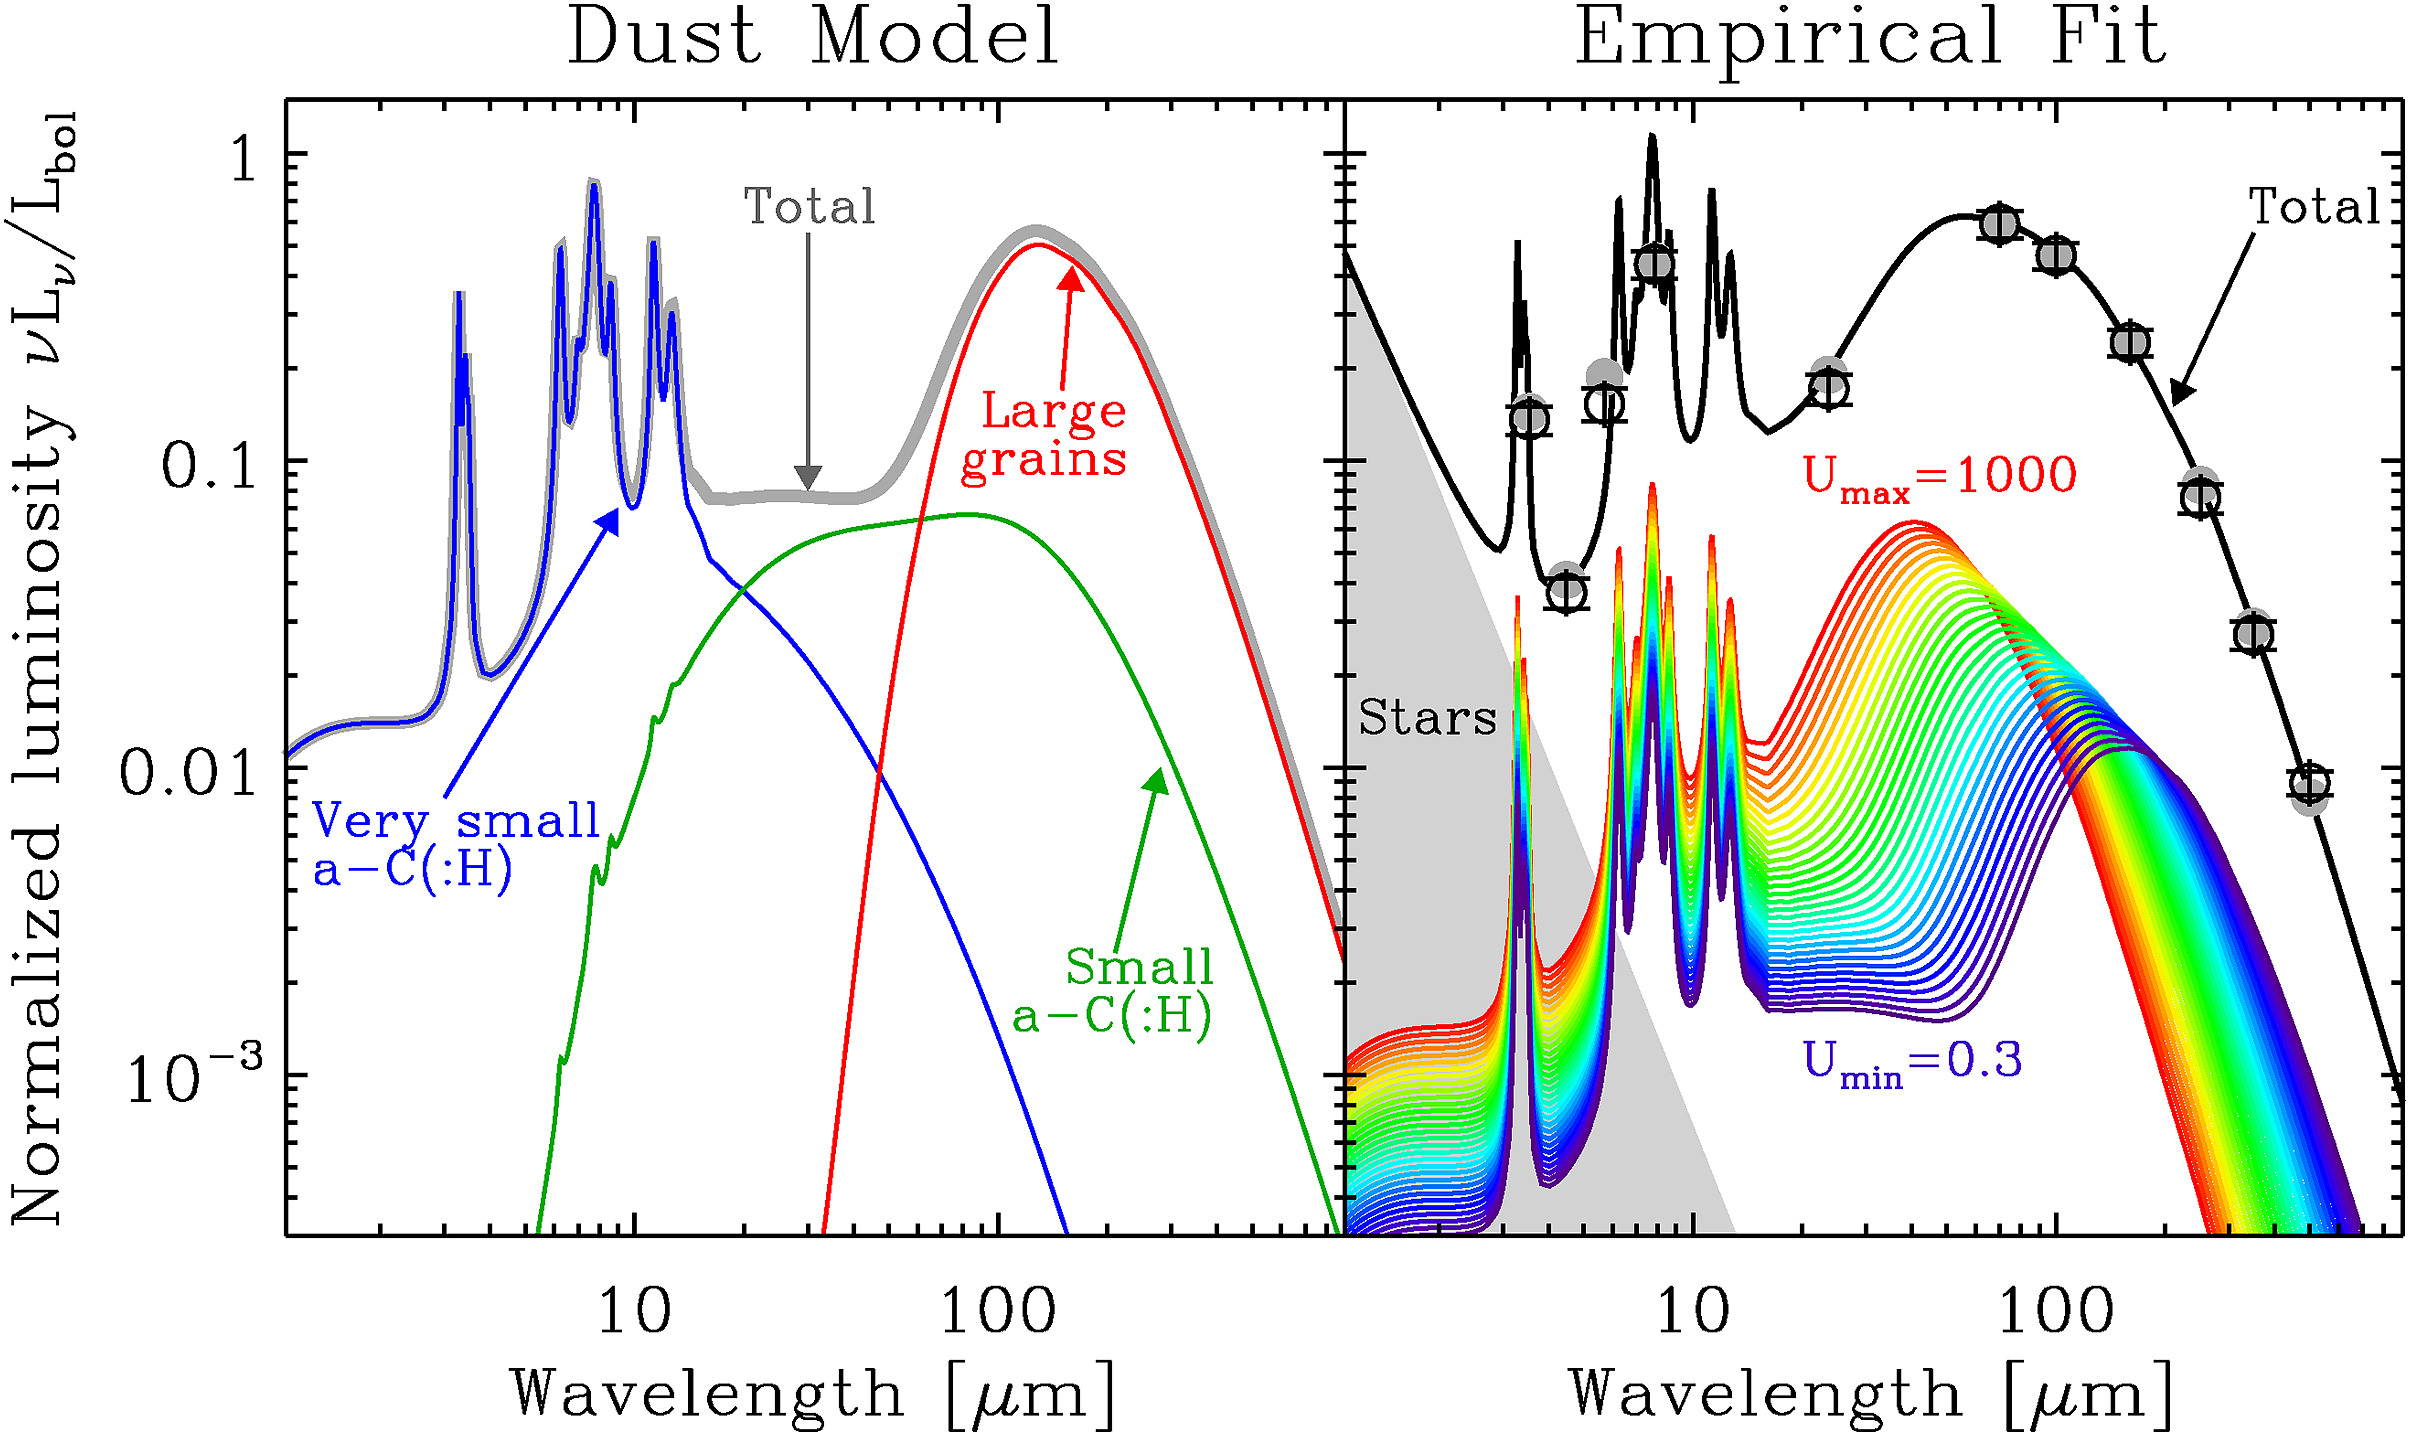
\includegraphics[width=14cm]{figures/GalaxySED_model.jpg}
    \caption{\footnotesize{Dust SED modelling. \textbf{Left:} Dust model of Jones et al. (2017) uniformly illuminated by the solar neighborhood radiation field ($U=1$). \textbf{Right:} An example of SED fit. The observations are the open circles with error bars (simulated data, for demonstration). The filled circles are the synthetic photometry of the model. The total model is the sum of uniformly illuminated SEDs with radiation field intensity ranging between $U_{\rm min}$ and $U_{\rm max}$ (rainbow curves). Figure taken from Galliano (2017).}}
    \label{fig:dustpah}
\end{figure}

{\noindent}The left panel of Figure \ref{fig:dustpah} shows the dust mixture, heated by the solar neighborhood radiation field ($U=1$). The far-IR bump is emitted by the large grains (silicates and ${\rm a-C(:H)}$), at thermal equilibrium with the radiation field. The mid-IR continuum is carried by out-of-equilibrium small ${\rm a-C(:H)}$ (radius  $a\lesssim20\,{\rm nm}$). The aromatic features are carried by the smallest ${\rm a-C(:H)}$ (radius $a\lesssim1.5\,{\rm nm}$).

{\noindent}Such a dust model can not be used, as is, to fit the SED of galaxies, since there can be significant mixing of physical conditions in the beam or along the line of sight. Ideally, we should model the radiative transfer inside the object, but we usually lack the knowledge of its actual 3D structure. An alternative is to empirically account for the mixing, focusing only on quantities that are weakly dependent on radiative transfer processes.

{\noindent}The far-IR peak is mainly emitted by large grains at thermal equilibrium. Thus, its spectrum does not depend on the spectral shape of the incident radiation field, as it depends only on the total absorbed power. On the contrary, the spectral shape is important for small stochastically heated grains, as their temperature distribution depends on the mean photon energy. Fortunately, these grains do not account for a large fraction of the mass. However, it is not the case for the carriers of the aromatic features, since they are effectively heated by a narrower wavelength range of photons.

{\noindent}SED models being highly non-linear, several degeneracies and biases are encountered with a classical $\chi^2$ minimization fit. This is well-known for modified black body models, where the monochromatic luminosity is parameterized by the dust mass ($M_{\rm dust}$), the equilibrium temperature ($T_{\rm dust}$), and the emissivity index ($\beta$):

\begin{align*}
    L_\nu = M_{\rm dust} 4\pi\kappa_0 \left(\frac{\nu}{\nu_0}\right)^\beta B_\nu (T_{\rm dust},\nu) ~ [{\rm W}],
\end{align*}

{\noindent}where $\kappa_0$ is the opacity at frequency $\nu$, and $B_\nu$ is the Planck function. There are also biases induced by our ignorance of the origin of certain physical processes. In particular, the ``\textbf{submm excess}'' is an emission excess particularly strong beyond $500\,\mu{\rm m}$ in low-metallicity environments, but it has also been detected in the MW. It can not be accounted for by regular dust models, free-free, synchrotron and molecular line emission. Its origin is still debated: (i) very cold dust, although unlikely; (ii) magnetic grains; (iii) temperature dependent grain emissivity; or (iv) intrinsic grain optical properties. The only way to avoid this excess is to not use constraints beyond $500\,\mu{\rm m}$.

{\noindent}Figure \ref{fig:galaxySEDappmodel} demonstrates a panchromatic SED model applied to a galaxy and Figure \ref{fig:galaxySEDgeometry} illustrates its geometry.

\begin{figure}[h]
    \centering
    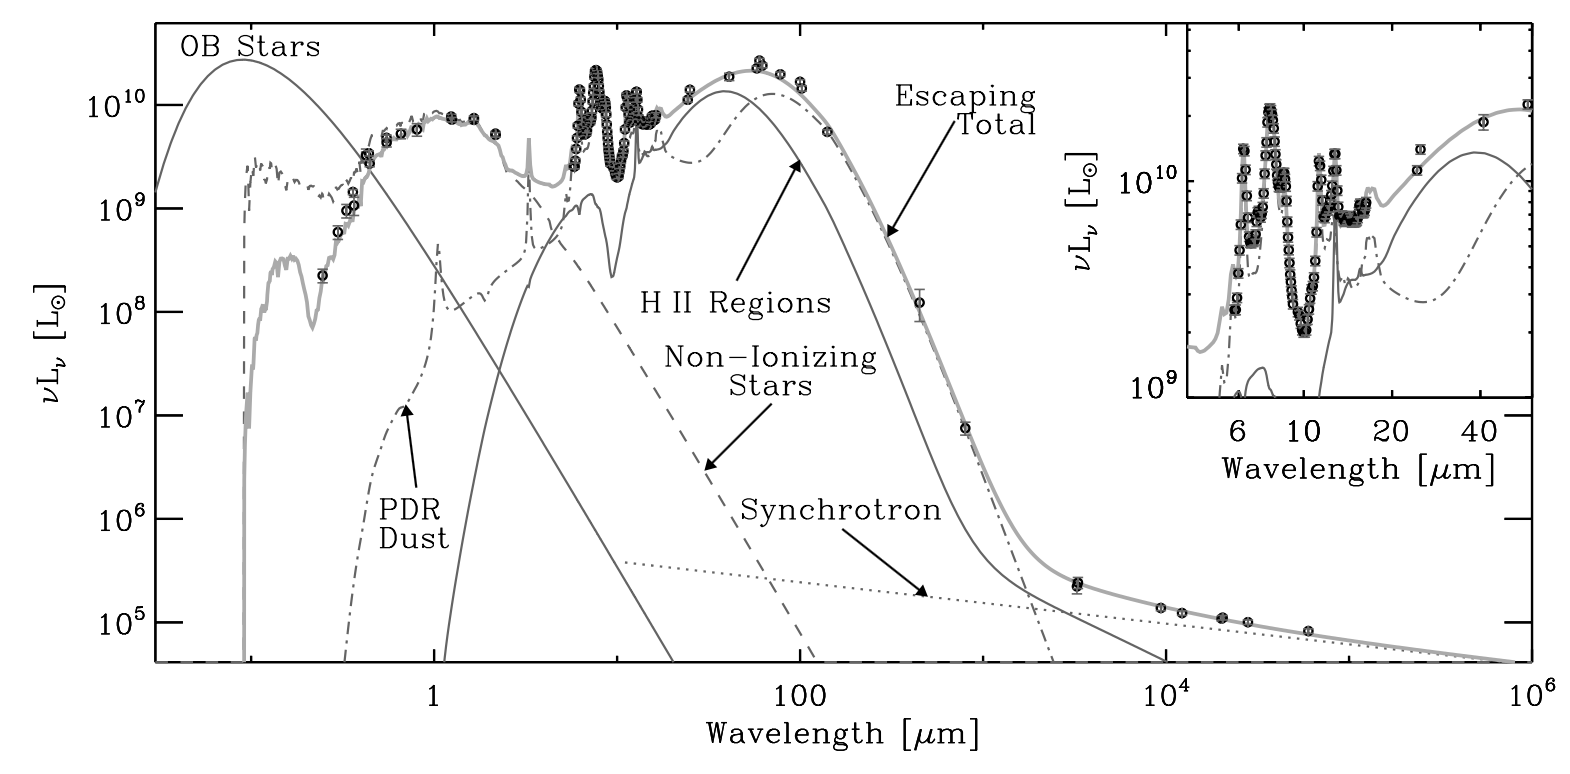
\includegraphics[width=14cm]{figures/GalaxySED_appmodel.png}
    \caption{\footnotesize{Demonstration of a panchromatic SED model applied to a galaxy. Figure taken from Galliano (2008).}}
    \label{fig:galaxySEDappmodel}
\end{figure}

\begin{figure}[t!]
    \centering
    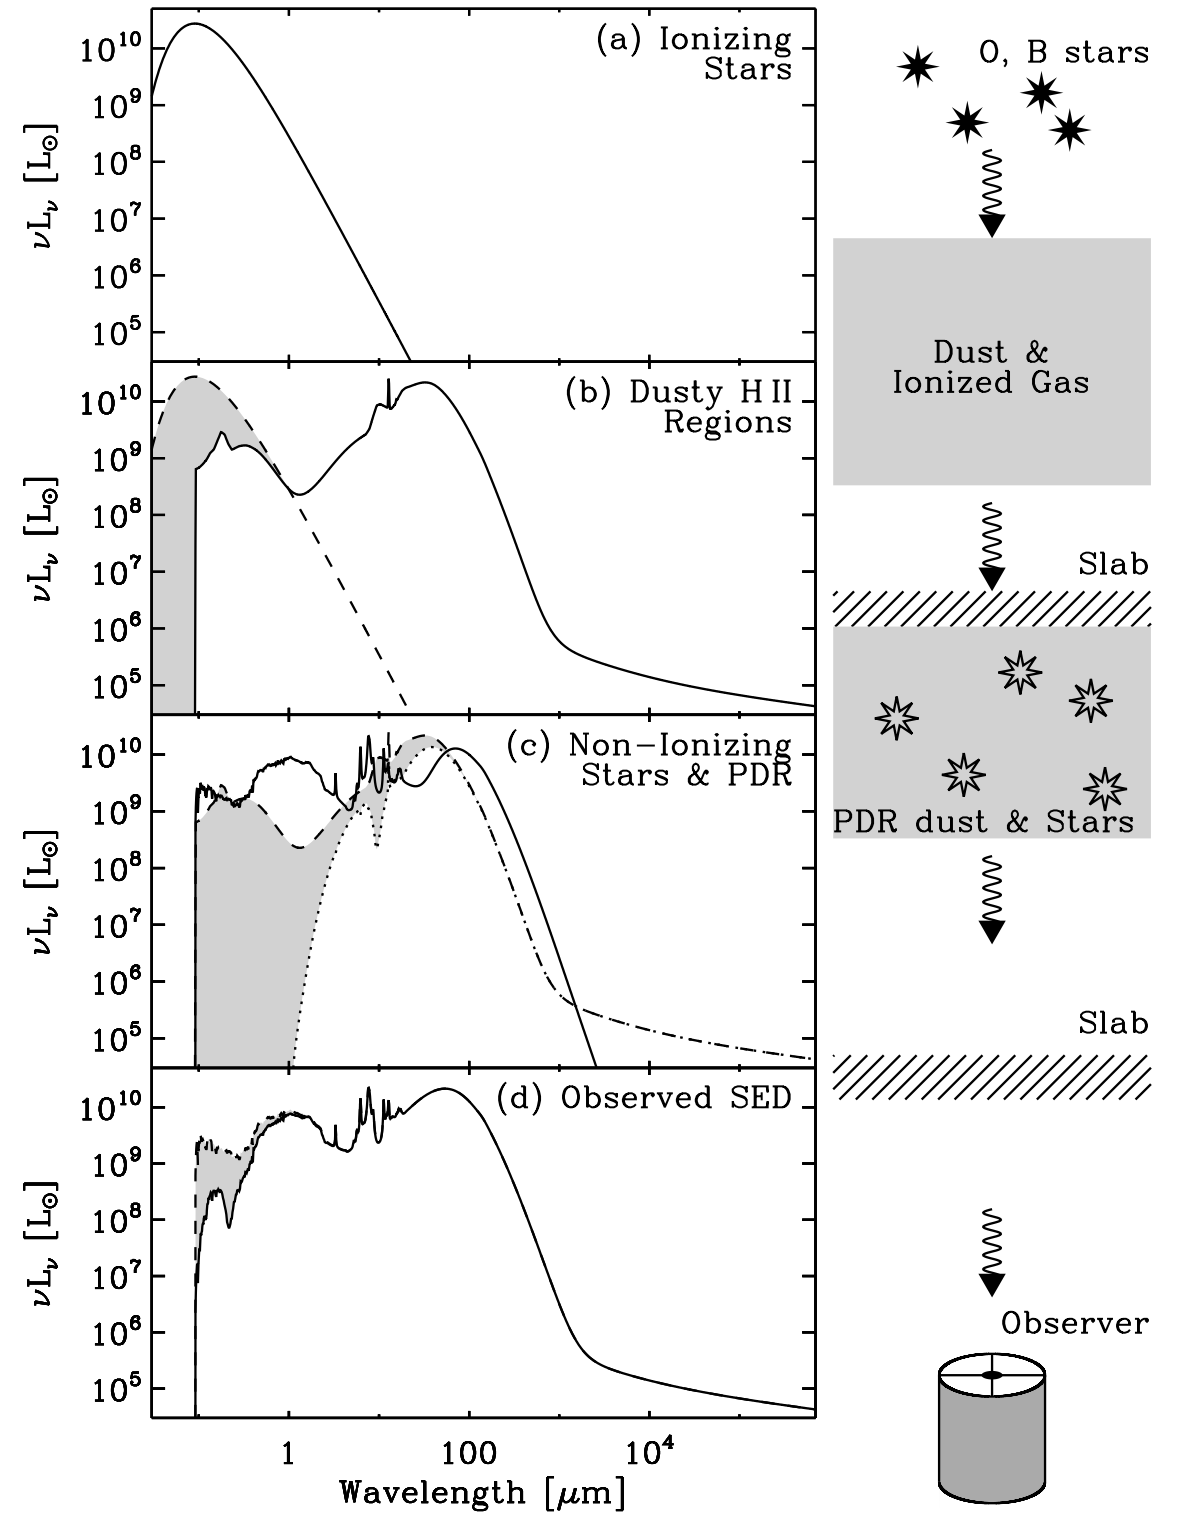
\includegraphics[width=14cm]{figures/GalaxySED_geometry.png}
    \caption{\footnotesize{Illustration of the geometry of a panchromatic SED model. The left panels, from top to bottom, show the combination of the various SED building blocks moving from the massive star clusters to the observer. The solid lines are the total SED at each step; the dashed lines are the SED of the previous step; and the part of the SED that has been absorbed is shown in gray. The right panel illustrates the path of the photons from the star clusters to the observer. Figure taken from Galliano (2008).}}
    \label{fig:galaxySEDgeometry}
\end{figure}

\newpage
\subsubsection{Follow-up Questions}

\begin{itemize}
    \item How do the relative heights of the optical/FIR peaks change?
\end{itemize}

% --------------------------------------------------------------
%               12. 
% --------------------------------------------------------------

\newpage
\subsection{Question 12}

How many stars does one expect to find within $100\,\mathrm{pc}$ of the Sun? If all stars are distributed evenly across the galaxy, how many of these will be B spectral type or earlier? How many are younger than $100\,\mathrm{Myrs}$?

\subsubsection{Short answer}

Answer.

\subsubsection{Additional context}

Additional context.

\subsubsection{Follow-up Questions}

\begin{itemize}
    \item Justify the assumptions made and explain why they do not match observations (e.g., number density of stars in the MW is not a flat distribution, the SFR isn't constant etc.).
    \item Where are most B-type and other early-type stars actually found?
    \item How do we know how many stars are in the MW?
    \item How do we measure the IMF?
    \item Are high- or low-mass stars more important to constrain the total number of stars?
    \item How many B stars are visible from your backyard? Are there any star forming regions visible from your backyard?
\end{itemize}

% --------------------------------------------------------------
%               13. 
% --------------------------------------------------------------

\newpage
\subsection{Question 13}

Describe what happens as a cloud starts to collapse and form a star. What is the difference between the collapse and contraction stages? What happens to the internal temperature in both? When does the contraction phase end, and why does the end point depend on the mass of the object?

\subsubsection{Short answer}

Answer.

\subsubsection{Additional context}

Gravity is responsible for gathering gas into self-gravitating structures ranging in size from stars to giant molecular cloud complexes. Star formation involves extreme compression: part of a gas cloud collapses from a size $\sim10^{18}\,{\rm cm}$ down to a stellar size, $\sim10^{11}\,{\rm cm}$, with an accompanying increase in density by a factor $\sim10^{21}$.

{\noindent}Here, we consider the conditions necessary for gravitational collapse to occur. There are several barriers to gravitational collapse. Gravity must of course overcome the resistance of pressure, both gas pressure and magnetic pressure. If the collapse is to produce a huge increase in density (as is necessary to form a star), then nearly all of the angular momentum in the collapsing gas must be transferred to nearby material. Last, the observed magnetic fields of young stars require that most of the magnetic field lines initially present in the gas not be swept into the forming protostar.

{\noindent}The \textbf{Jeans instability} occurs for a \textbf{Jeans length}

\begin{align*}
    \lambda > \lambda_J \equiv \frac{2\pi}{\kappa_J} = \sqrt{\frac{\pi c_s^2}{G\rho_0}} ~ [{\rm m}],
\end{align*}

{\noindent}where

\begin{align*}
    k_J \equiv \sqrt{\frac{4\pi G\rho_0}{c_s^2}} ~ [{\rm m^{-1}}].
\end{align*}

{\noindent}The \textbf{Jeans mass} is defined as

\begin{align*}
    M_J &\equiv \frac{4\pi}{3}\rho_0 \left(\frac{\lambda_J}{2}\right)^3 ~ [{\rm M_\odot}] \\
        &= \frac{1}{8} \left(\frac{\pi kT}{\mu G}\right)^{3/2} \rho_0^{-1/2} ~ [{\rm M_\odot}] \\
        &= 0.32 \left(\frac{T}{10\,{\rm K}}\right)^{3/2} \left(\frac{m_{\rm H}}{\mu}\right)^{3/2} \left(\frac{10^6\,{\rm cm^{-3}}}{n_{\rm H}}\right)^{1/2}  ~ [{\rm M_\odot}].
\end{align*}

{\noindent}It is gratifying that when we substitute densities and temperatures observed for quiescent dark clouds, we find a mass typical of stars! If we plug in some typical numbers for a GMC, $c_s=0.2\,{\rm km\,s^{-1}}$ and $\rho_0=100\,m_p$, we get $\lambda_J=3.4\,{\rm pc}$. Since every GMC we have seen is larger than this size, and there are clearly always perturbations present, this means that molecular clouds cannot be stabilized by gas pressure against collapse. 

{\noindent}In the limit of $k\ll k_J$ (long wavelength), the exponentiation time or ``\textbf{growth time}'' is

\begin{align*}
    \tau_J = \frac{1}{k_Jc_s} = \frac{1}{\sqrt{4\pi G\rho_0}} = 2.3\times10^4 \left(\frac{n_{\rm H}}{10^6\,{\rm cm^{-3}}}\right)^{-1/2} ~ [{\rm yr}].
\end{align*}

{\noindent}To understand the value of the growth time $\tau_J$, note that a uniform pressureless sphere of initially stationary gas with density $\rho_0$ will collapse with all shells reaching the center simultaneously in a finite time known as the \textbf{free-fall time}

\begin{align*}
    \tau_{\rm ff} = \sqrt{\frac{3\pi}{32G\rho_0}} = 4.4\times10^4 \left(\frac{n_{\rm H}}{10^6\,{\rm cm^{-3}}}\right)^{-1/2} ~ [{\rm yr}].
\end{align*}

{\noindent}The free-fall time $\tau_{\rm ff}$ is only slightly longer than the Jeans growth time $\tau_J$.

{\noindent}Self-gravitating density peaks within an isolated ``dark cloud'' are usually referred to as \textbf{cores}. The cores have masses of order $0.3\,{\rm M_\odot}$ to $10\,{\rm M_\odot}$. Each core is likely to form a single star or a binary star.

{\noindent}In the case of GMCs, the term \textbf{clump} is used to refer to self-gravitating regions with masses as large as $\sim10^3\,{\rm M_\odot}$. Clumps may or may not be forming stars; those that are, are termed \textbf{star-forming clumps}. Such clumps will generally contain a number of cores.

{\noindent}When a core becomes gravitationally unstable, it will begin to collapse. Exactly how this collapse proceeds is uncertain in detail, but we think we understand the overall outlines.

{\noindent}During the initial stages, radiative cooling in molecular lines is able to keep the gas cool. As a result, the gas pressure remains unimportant during this phase, and the matter moves inward nearly in free-fall. The velocities at this stage are not large,

\begin{align*}
    v &\lesssim \sqrt{\frac{GM_c}{R_c}} = \left(\frac{4\pi}{3}\right)^{1/3} G^{1/2} M^{1/3} \rho_c^{1/6} \\
    &\approx 0.4 \left(\frac{M_c}{{\rm M_\odot}}\right)^{1/3} n_6^{1/6} ~ [{\rm km\,s^{-1}}],
\end{align*}

{\noindent}where $M_c$ and $\rho_c=1.4n_{\rm H}m_{\rm H}$ are the mass and density of the core, and $n_{\rm H}=10^6n^6\,{cm^{-3}}$.

{\noindent}Because the density is higher in the interior, the free-fall time is shortest there, and the collapse proceeds in an ``inside-out'' manner, with the center collapsing first, and the outer material later falling onto the central matter.

{\noindent}If cores had no angular momentum, and if magnetic fields were negligible, the collapse process would be relatively simple to understand and model. However, molecular clouds appear to have magnetic energies comparable to the kinetic energy (contributed mainly by the ``turbulent'' motions), and sufficient angular momentum to become dynamically important long
before stellar densities are reached. 

{\noindent}The infalling gas will generally have nonzero angular momentum, and (if it remains cold) the material will collapse to form a rotationally supported disk, with the material with the lowest specific angular momentum collected in a ``\textbf{protostar}'' at the center of the disk. Energy is dissipated as the infalling gas hits the disk. Angular momentum transport (due to the \textbf{magneto-rotational instability} (MRI) if the gas is sufficiently ionized, or due to gravitational torques or turbulent viscosity if the ionization is too low to support the MRI) will cause some material in the disk to move inward, with additional release of gravitational energy. The energy so released will heat the disk, and will be radiated away.

{\noindent}The dominant sources of energy are (1) the gravitational energy released as material is added to the protostar and as the protostar contracts, and (2) the energy released when the protostar is able to ignite fusion reactions to first ``burn'' deuterium, and then hydrogen. The protostar will have a significant luminosity, allowing it and the surrounding core to be observed as a luminous infrared source.

{\noindent}\textbf{Thermodynamics of a Collapsing Core}: We will now focus on the structure and evolution of protostars. Our goal will be to understand when and why collapse stops to form a pressure-supported object, and how those objects subsequently evolve into main sequence stars. This chapter focuses on
the dynamics and thermal behavior of the material at the center of a collapsing core as it settles into something we can describe as a star, and on the structure of the envelope around this protostar. Later we will focus on the evolution of this object, both internally and in its appearance on the HR diagram.

{\noindent}\textbf{Thermodynamics of a Collapsing Core}: We will begin by considering what happens at the center of a collapsing core where the density in the center is rising rapidly as it collapses. We would like to understand the structure forming at the center of this collapsing object.

{\noindent}\textbf{The Isothermal-Adiabatic Transition}: The first important point to make is the assumption of isothermality for cores must break down at some point. Even at low density there are minor deviations from isothermality that result from the changeover in heating and cooling processes, but these are fairly minor, in the sense that they are unable to significantly affect collapse. 

{\noindent}In contrast, if the gas is not able to radiate at all, it will behave adiabatically. This means it will approach a polytrope with $\gamma=7/5$ or $\gamma=5/3$, depending on whether the gas temperature is high enough to excite the internal quantum mechanical states of H$_2$ or not. (In actuality the $\gamma$ for H$_2$ is more complicated than that, but that doesn't really matter for our purposes.) Either one is $>4/3$, and thus sufficient to halt collapse.

{\noindent}Let us make some estimates of when deviations from isothermality that are significant enough to put us into this regime will occur. Since we are dealing with the collapse of the first region to fall in, we can probably safely assume that this material has very low angular momentum and treat the collapse as spherical -- higher angular momentum material will only fall in later, since removal of angular momentum by the disk takes a while.

{\noindent}Let $e_{\rm th}$ be the \textbf{thermal energy per unit mass} of a particular gas parcel, and let $\Gamma$ and $\Lambda$ be the \textbf{rates of change in} $\mathbf{e_{\rm th}}$ \textbf{due to heating and cooling processes}, i.e.:

\begin{align*}
    \frac{{\rm d}e_{\rm th}}{{\rm d}} = \Gamma - \Lambda ~ [{\rm J\,kg^{-1}\,s^{-1}}].
\end{align*}

{\noindent}At high densities inside a core immediately before a central star forms and begins to radiate, the dominant source of energy is adiabatic compression of the gas. The first law of thermodynamics tells us that the \textbf{heating rate due to compression} is

\begin{align*}
    \Gamma = -p \frac{{\rm d}}{{\rm d}t} \left(\frac{1}{\rho}\right) ~ [{\rm J\,kg^{-1}\,s^{-1}}],
\end{align*}

{\noindent}where $p$ and $\rho$ are the gas pressure and density. Since $1/\rho$ is the specific volume, meaning the volume per unit mass occupied by the gas, this term is just $p\,{\rm d}V$, the work done on the gas in compressing it. If the gas is collapsing in free-fall, the compression timescale is about the free-fall timescale, $t_{\rm ff} \sim 1/\sqrt{G\rho}$, so we expect 

\begin{align*}
    \frac{{\rm d}}{{\rm d}t} \left(\frac{1}{\rho}\right) = C_1 \sqrt{\frac{4\pi G}{\rho}} 
\end{align*}

{\noindent}where $C_1$ is a number of order unity that will depend on the exact collapse solution, and the factor of $\sqrt{4\pi}$ has been inserted for future convenience. Writing $p=\rho c_s^2$ and plugging this into the heating rate, we get

\begin{align*}
    \Gamma = C_1c_s^2 \sqrt{4\pi G\rho} ~ [{\rm J\,kg^{-1}\,s^{-1}}].
\end{align*}

{\noindent}The main cooling source is thermal emission by dust grains, which at the high densities with which we are concerned are thermally very well coupled to the gas. Let us first consider the gas where the gas is optically thin to this thermal radiation. In this case the cooling rate per unit mass is simply given by the rate of thermal emission,

\begin{align*}
    \Lambda_{\rm thin} = 4\kappa_P\sigma T^4 ~ [{\rm J\,kg^{-1}\,s^{-1}}],
\end{align*}

{\noindent}where $\sigma$ is the Stefan-Boltzmann constant and $\kappa_P$ is the Planck mean opacity of the dust grains. As long as $\Lambda>\Gamma$, the gas will remain isothermal. (Strictly speaking if $\Lambda>\Gamma$ the gas will cool, but that's because we've left out other sources of heating, such as cosmic rays and the fact that the protostar is bathed in a background IR radiation field from other stars.)

{\noindent}If we equate the heating and cooling rates, using for $T$ the temperature in the isothermal gas, we therefore will obtain a characteristic density beyond which the gas can no longer remain isothermal. Doing so gives

\begin{align*}
    \rho_{\rm thin} &= \frac{4}{\pi} \frac{\kappa_P^2\sigma^2\mu^2T^4}{C_1^2Gk_B^2} \\
    &= 5\times10^{-15} C_1^{-2} \left(\frac{100\,\kappa_P}{{\rm cm^2\,g^{-1}}}\right)^2 \left(\frac{T}{10\,{\rm K}}\right)^6 ~ [{\rm g\,cm^{-3}}],
\end{align*}

{\noindent}where $\mu$ is the mean mass per particle and we have set $c_s=\sqrt{k_BT/\mu}$. Thus we find that compressional heating and optically thin cooling to balance at about $10^{14}\,{\rm g\,cm^{-3}}$.

{\noindent}A second important density is the one at which the gas starts to become optically thick to its own re-emitted IR radiation. Suppose that the optically thick region at the center of our core has some mean density $\rho$ and radius $R$. The condition that the optical depth across it be unity then reduces to

\begin{align*}
    2\kappa\rho R \approx 1.
\end{align*}

{\noindent}If this central region corresponds to the size of the region that is no longer in free-fall collapse and is instead thermally supported, then its size must be comparable to the Jeans length at its lowest temperature, i.e., $R\sim\lambda_J = \sqrt{\pi c_s^2/G\rho}$. Thus we set

\begin{align*}
    R = C_2 \frac{2\pi c_s}{\sqrt{4\pi G\rho}} ~ [{\rm pc}],
\end{align*}

{\noindent}where C2 is again a constant of order unity.

{\noindent}Plugging this into the condition for optical depth unity, we derive the \textbf{characteristic density} at which the gas transitions from optically thin to optically thick:

\begin{align*}
    \rho_{\tau\sim1} &= \frac{1}{4\pi} C_2^{-2} \frac{\mu G}{\kappa_P^2k_BT} \\
    &= 1.5\times10^{-13} \left(\frac{100\,\kappa_P}{{\rm cm^2\,g^{-1}}}\right)^{-2} \left(\frac{T}{10\,{\rm K}}\right)^{-1} ~ [{\rm g\,cm^{-3}}].
\end{align*}

{\noindent}This is not very different from the value for $\rho_{\rm thin}$, so in general for reasonable collapse conditions we expect that cores transition from isothermal to close to adiabatic at a density of $\sim10^{-13}-10^{-14}\,{\rm g\,cm^{-3}}$.

{\noindent}It is worth noting that ratio of $\rho_{\rm thin}$ to $\rho_{\tau\sim1}$ depends extremely strongly on both $\kappa_P$ (to the 4th power) and T (to the 7th), so any small change in either can render them very different. For example, if the metallicity is super-solar then $\kappa_P$ will be larger, which will increase $\rho_{\rm thin}$ and decrease $\rho_{\tau\sim1}$ Similarly, if the region is somewhat warmer, for example due to the presence of nearby massive stars, then $\rho_{\rm thin}$ will increase and $\rho_{\tau\sim1}$ will decrease.

{\noindent}If $\rho_{\tau\sim1}<\rho_{\rm thin}$ the collapsing gas will become optically thick before heating becomes faster than optically thin cooling. In this case we must compare the heating rate due to compression with the cooling rate due to optically thick cooling instead of optically thin cooling. Optically thick cooling is determined by the rate at which radiation can diffuse out of the core. If we have a central region of optical depth $\tau\gg1$, the effective \textbf{speed of the radiation} moving through it is $c/\tau$, so the time required for the radiation to diffuse out is

\begin{align*}
    t_{\rm diff} = \frac{\ell\tau}{c} = \frac{\kappa_P\rho\ell^2}{c} ~ [{\rm yr}],
\end{align*}

{\noindent}where $\ell$ is the \textbf{characteristic size} of the core.

{\noindent}Inside the optically thick region matter and radiation are in thermal balance, so the radiation energy density approaches the blackbody value $aT^4$. The radiation energy per unit mass is therefore $aT^4/\rho$. Putting all this together, and taking $\ell=2R$ as we did before in computing $\rho_{\tau\sim1}$, the optically thick cooling rate per unit mass is

\begin{align*}
    \Lambda_{\rm thick} = \frac{aT^4\rho}{t_{\rm diff}} = \frac{\sigma T^4}{\kappa_P\rho^2R^2} ~ [{\rm J\,kg^{-1}\,s^{-1}}],
\end{align*}

{\noindent}where $\sigma=ca/4$. If we equate $\Lambda_{\rm thick}$ and $\Gamma$, we get the characteristic density where the gas becomes non-isothermal in the optically thick regime

\begin{align*}
    \rho_{\rm thick} &= \left(\frac{C_1^2G\sigma^2\mu^4T^4}{4\pi^3C_2^4k_B^4\kappa_P^2}\right)^{1/3} \\
    &= 5\times10^{-14} \left(\frac{C_1^{2/3}}{C_2^{4/3}}\right) \left(\frac{100\,\kappa_P}{{\rm cm^2\,g^{-1}}}\right)^{-2/3} \left(\frac{T}{10\,{\rm K}}\right)^{4/3} ~ [{\rm g\,cm^{-3}}]
\end{align*}

{\noindent}This is much more weakly dependent on $\kappa_P$ and $T$, so we can now make the somewhat more general statement that, even for super-solar metallicity or warmer regions, we expect a transition from isothermal to adiabatic behavior somewhere in the vicinity of $10^{-14}-10^{-13}\,{\rm g\,cm^{-3}}$.

{\noindent}\textbf{The first core}: The transition to an adiabatic equation of state, with $\gamma>4/3$, means that the collapse must at least temporarily halt. The result will be a hydrostatic object that is supported by its own internal pressure. This object is known as the \textbf{first core}, or sometimes a \textbf{Larson's first core}, after Richard Larson, who first predicted this phenomenon.

{\noindent}We can model the first core reasonably well as a simple polytrope, with index $n$ defined by $n=1/(\gamma-1)$. At low mass when the temperature in the first core is low $\gamma\approx5/3$ and $\gamma\approx3/2$, and for a more massive, warmer core $\gamma\approx7/5$ ($n\approx5/2$). For a polytrope of central density $\rho_c$, the radius and mass are

\begin{align*}
    R &= a\xi_1 ~ [{\rm pc}]\\
    M &= -4\pi a^3\rho_c \left(\xi^2\frac{{\rm d}\theta}{{\rm d}\xi}\right)_1 ~ [{\rm M_\odot}],
\end{align*}

{\noindent}where $\xi=r/a$ is the \textbf{dimensionless radius}, $\theta=(\rho/\rho_c)^{1/n}$ is the \textbf{dimensionless density}, the subscript $1$ refers to the value at the edge of the sphere (where $\theta=0$), the factors $\xi_1$ and $(\xi{\rm d}\theta/{\rm d}\xi)_1$ can be determined by integrating the \textbf{Lane-Emden equation}, and the scale factor $a$ is defined by

\begin{align*}
    a = \sqrt{\frac{(n+1)K}{4\pi G}\rho_c^{(1-n)/n}} ~ [{\rm pc}].
\end{align*}

{\noindent}The factor $K=p/\rho^\gamma$ is the \textbf{polytropic constant}, which is determined by the specific entropy of the gas.

{\noindent}For our first core, the specific entropy will just be determined by the density at which the gas transitions from isothermal to adiabatic. If we let $\rho_{\rm ad}$ be the density at which the gas becomes adiabatic, then the pressure at this density is $p=\rho_{\rm ad}c_{s0}^2$, where $c_{s0}$ is the sound speed in the isothermal phase, and $K=c_{s0}^2\rho_{\rm ad}^{1-\gamma}$. For $\gamma=5/3$ ($n=1.5$) we have $\xi_1=3.65$ and ($\xi{\rm d}\theta/{\rm d}\xi)_1=2.71$, and plugging in we get

\begin{align*}
    R &= 2.2 \left(\frac{10^{10}\rho_c}{{\rm g\,cm^{-3}}}\right)^{1/6} \left(\frac{T}{10\,{\rm K}}\right)^{1/2} \left(\frac{10^{13}\rho_{\rm ad}}{{\rm cm^{-3}}}\right)^{-1/3} ~ [{\rm AU}] \\
    M &= 0.059 \left(\frac{10^{10}\rho_c}{{\rm g\,cm^{-3}}}\right)^{1/6} \left(\frac{T}{10\,{\rm K}}\right)^{1/2} \left(\frac{10^{13}\rho_{\rm ad}}{{\rm cm^{-3}}}\right)^{-1/3} ~ [{\rm M_\odot}].
\end{align*}

{\noindent}We can obtain very similar numbers by plugging in for $\gamma=7/5$ ($n=2.5$). These results show that the first core is an object a few AU in size, with a mass of a few hundredths of a solar mass.

{\noindent}\textbf{Second collapse}: The first core is a very short-lived phase in the evolution of the protostar. To see why, let us estimate its temperature. The temperature inside the sphere rises as $T\propto\rho^{\gamma-1}$, so the central temperature is

\begin{align*}
    T_c = T_0 \left(\frac{\rho_c}{\rho_{\rm ad}}\right) ^{\gamma-1} ~ [{\rm K}],
\end{align*}

{\noindent}where $T_0$ is the temperature in the isothermal phase. Thus the central temperature will be higher than the boundary temperature by a factor that is determined by how high the central density has risen, which in turn will be determined by the amount of mass that has accumulated on the core.

{\noindent}In general we have $M\propto
rho_c^{(3+n)/(2n)}$, or $M\propto\rho_c^{(3\gamma-2)/2}$. We also have $T_c\propto\rho_c^{\gamma-1}$. Combining these results, we get

\begin{align*}
    T_c \propto M^{(2\gamma-2)/(3\gamma-2)} ~ [{\rm K}].
\end{align*}

{\noindent}The exponent is $0.44$ for $\gamma=5/3$ and $0.36$ for $\gamma=7/5$.

{\noindent}Plugging in some numbers, $M=0.06\,{\rm M_\odot}$, $\rho_{\rm ad}=10^{-13}\,{\rm g\,cm^{-3}}$, and $\gamma=5/3$ gives $\rho_c=10^{-10}{\rm g\,cm^{-3}}$ and $T_c=1000\,{\rm K}$. Thus we see that by the time anything like $M=0.1\,{\rm M_\odot}$ of material has accumulated on the first core, compression will have caused its central temperature to rise to $1000\,{\rm K}$ or more.

{\noindent}This causes yet another change in the thermodynamics of the gas, because all the hydrogen is still molecular, and molecular hydrogen has a binding energy of $4.5\,{\rm eV}$. In comparison, the kinetic energy per molecule for molecular hydrogen at a temperature $T$ is $3k_BT=0.26T_3\,{\rm eV}$, where $T_3=T/(1000\,{\rm K})$. At $1000\,{\rm K}$ this means that the mean molecule still has only $\sim5\%$ of the kinetic energy that would be required to dissociate it. However, there is a non-negligible tail of the Maxwellian distribution that is moving fast enough for collisions to produce dissociation. Each of these dissociative collisions removes $4.5\,{\rm eV}$ from the kinetic energy budget of the gas and puts it into chemical energy instead. Since dissociations are occurring on the tail of the Maxwellian, any slight increase in the temperature dramatically increases the dissociation rate, moving even more kinetic energy into chemical energy.

{\noindent}This effectively acts as a thermostat for the gas, in much the same way that a boiling pot of water stays near the boiling temperature of water even when energy is added, because all the extra energy that is provided goes into changing the chemical state of the water rather than raising its temperature. Detailed numerical calculations of this effect show that at temperatures above $1000-2000\,{\rm K}$, the equation of state becomes closer to $T\propto\rho^{0.1}$, or $\gamma=1.1$. This is again below the critical value of $\gamma=4/3$ required to have a hydrostatic object, and as a result the center of the first core again goes into something like free-fall collapse.

{\noindent}This is called the \textbf{second collapse}. The time required for it is set by the free-fall time at the central density of the first core, which is only a few years. This collapse continues until all the hydrogen dissociates. The hydrogen also ionizes during this collapse, since the ionization potential of $13.6\,{\rm eV}$ isn't very different from the dissociation potential of $4.5\,{\rm eV}$. Only once all the hydrogen is dissociated and ionized can a new hydrostatic object form.

{\noindent}At this point the gas is warmer than $\sim10^4\,{\rm K}$, is fully ionized, and the new hydrostatic object is a true protostar. It is supported by degeneracy pressure at first when its mass is low, and then as more mass arrives it heats up and becomes supported by thermal pressure.

{\noindent}An important point to make there is that this discussion implies that brown dwarfs, at least those of sufficiently low mass, do not undergo a prompt second collapse. Instead, their first cores never accumulate enough mass to dissociate the molecules at their center. This isn't to say that dissociation never happens in them, and that second collapse never occurs. A brown dwarf-mass first core will still radiate from its surface and, lacking any internal energy source, this energy loss will have to be balanced by compression. As the gas compresses the temperature and entropy will rise, and, if the object does not become supported by degeneracy pressure first, the central temperature will eventually rise enough to produce second collapse. The difference for a brown dwarf is that this will only occur once slow radiative losses cause a temperature rise, which may take a very long time compared to formation. For stars, in contrast, there is enough mass to reach the critical temperature by compression during formation.

{\noindent}\textbf{Evolutionary phases for protostars}: There are generally a few distinct stages though with forming stars pass, which can be read off from how the radius evolves as the star gains mass. We will use as our primary example the case of a star undergoing hot accretion at $10^{-5}\,{\rm M_\odot\,yr^{-1}}$, as illustrated in Figure \ref{fig:RvsMprotostars}. However, note that the ordering of these phases we'll describe below can vary somewhat depending on the accretion rate and the boundary conditions assumed. Moreover, for low mass stars, some of the later phases may not occur at all, or occur only after the end of accretion.

\begin{figure}[h]
    \floatbox[{\capbeside\thisfloatsetup{capbesideposition={right,top},capbesidewidth=4cm}}]{figure}[\FBwidth]
    {\caption{\footnotesize{Kippenhahn and composition diagrams for a protostar accreting at $10^{-5}\,{\rm M_\odot\,yr^{-1}}$. In the top panel, the thick curve shows the protostellar radius as a function of mass, and gray and white bands show convective and radiative regions, respectively. Hatched areas show regions of D and H burning, as indicated. Thin dotted lines show the radii containing $0.1$, $0.3$, $1$, $3$, and $10\,{\rm M_\odot}$, as indicated. Shaded regions show four evolutionary phases: (I) convection, (II) swelling, (III) KH-contraction, and (IV) the main sequence. In the lower panel, the solid line shows the mean deuterium fraction in the star, normalized to the starting value, while the dashed line shows the D fraction only considering the convective parts of the star. The dot-dashed line shows the maximum temperature. Table taken from Krumholz (2015).}}
    \label{fig:RvsMprotostars}}
    {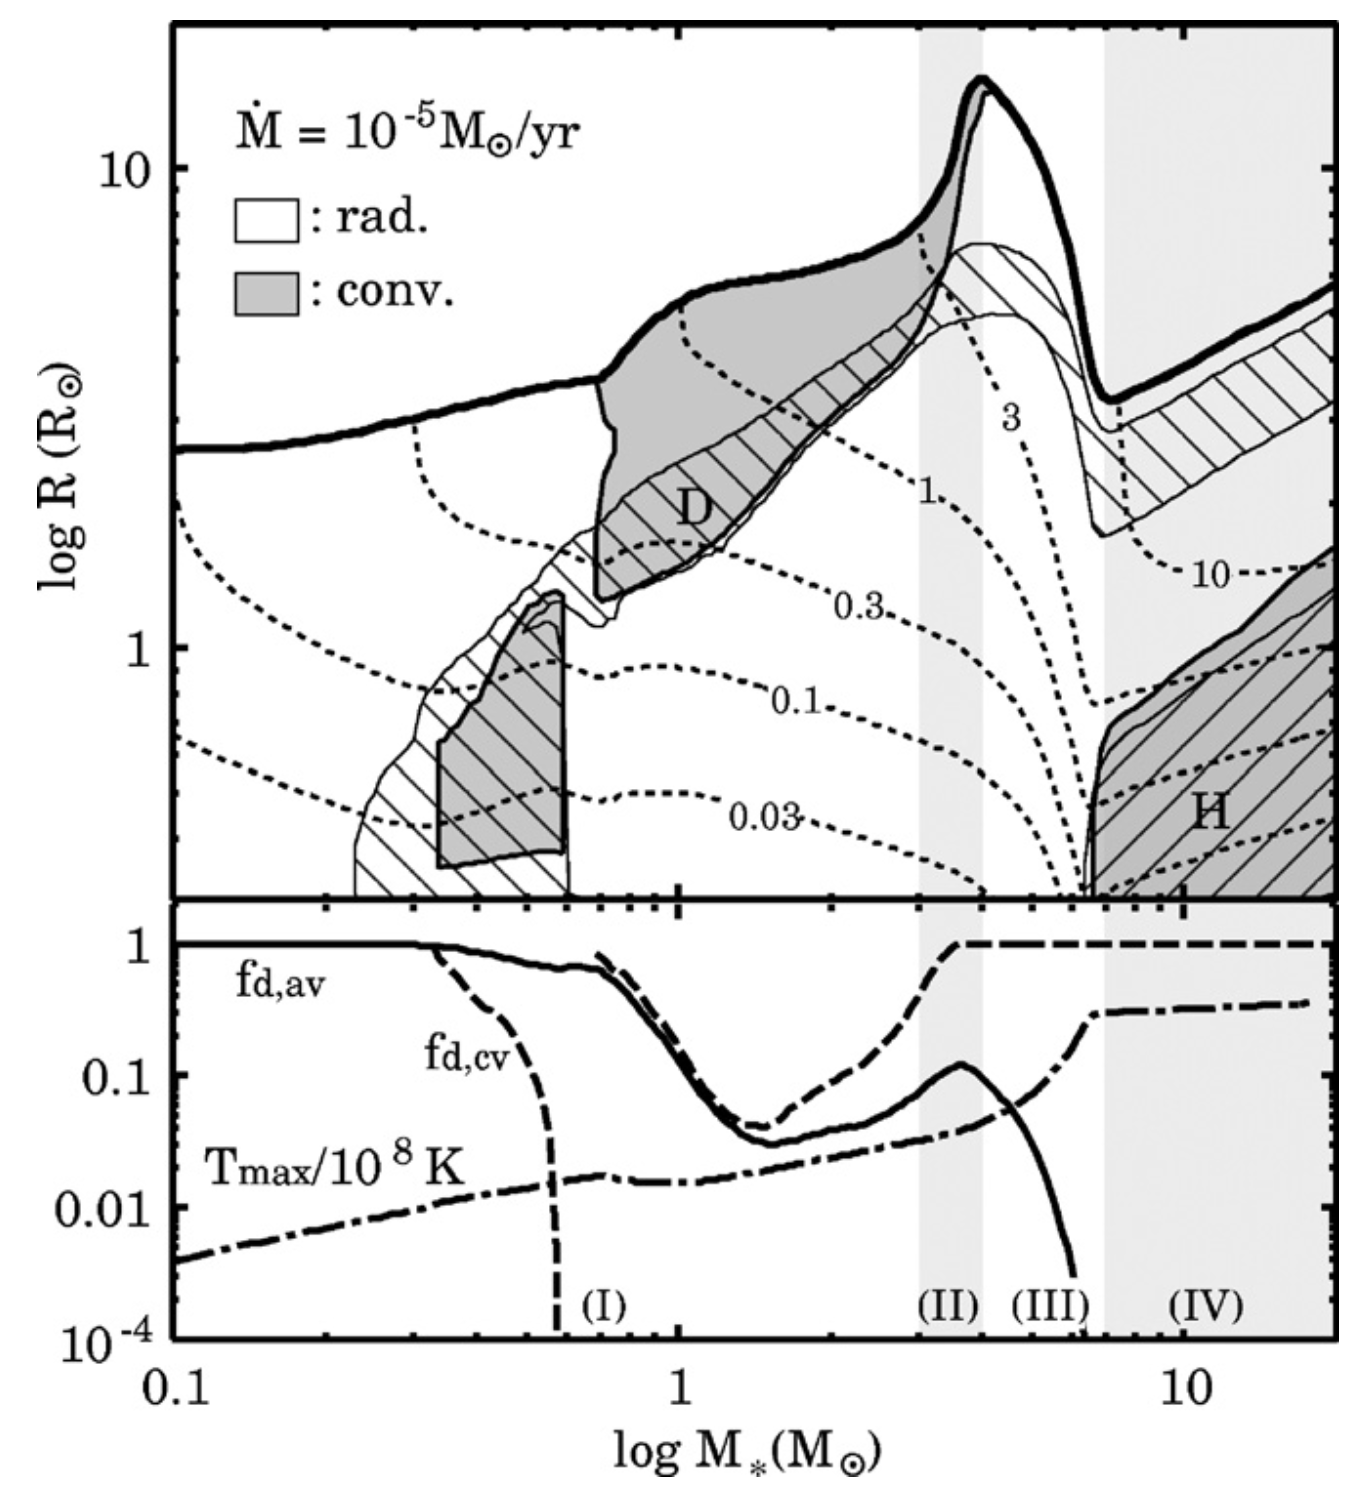
\includegraphics[width=10cm]{figures/RvsM_protostars.png}}
\end{figure}

{\noindent}The initial phase of evolution is visible in Figure \ref{fig:RvsMprotostars} as what takes place up to a mass of $\sim0.2\,{\rm M_\odot}$ for the example shown. The first thing that happens during this phase is that the star reaches a radius that is a function solely of $M_*$ and $\dot{M}_*$. This occurs regardless of the initial radius with which we initiate the model, as long as we are using the hot accretion boundary condition. The physical reason for this behavior is easy to understand. The radius of the star is determined by the entropy profile. High entropy leads to high radius. Since the internal energy generated by the star is small compared to the accretion power when the stellar mass is low (i.e., $L_{\rm bb}\ll L_{\rm acc}$), once gas is incorporated into the star it does not lose significant energy by radiation. The only entropy it loses is due to the radiation that occurs at the shock on the star's surface. We could have guessed this result from the large value of $t_{\rm KH}$ compared to the accretion time -- in effect, this means that, once a fluid element reaches the stellar surface it will be buried and reach a nearly constant entropy quite quickly. Consequently, we can treat the material falling onto the star during this phase as having an entropy per unit mass that depends only on two factors: (1) the entropy it acquires by striking the stellar surface, and (2) how much it radiates before being buried.

{\noindent}The latter factor is just determined by the accretion rate. Higher accretion rates bury accreted material more quickly, leaving it with higher entropy and producing larger radii. The former depends on the velocity of the infalling material just before it strikes the stellar surface, and thus on $v_{\rm ff} \propto \sqrt{M_*/R_*}$. However, this second factor self-regulates. If at fixed $M_*$, $R_*$ is very large, then $v_{\rm ff}$ is small, and the incoming material gains very little entropy in the shock. Small entropy leads to a smaller radius. Conversely, if $R_*$ is very small, then $v_{\rm ff}$ and the post-shock entropy will be large, and this will produce rapid swelling of the protostar. This effect means that the radius rapidly converges to a value that depends only on $M_*$ and
$\dot{M}_*$.

{\noindent}This self-regulation does not happen if the material is assumed undergoing cold accretion. In this case, the radial evolution of the star is determined solely by the amount of entropy that is assumed to remain in the accretion flow when it joins onto the star. One common practice is to assume that the entropy of the accreting material is equal to the entropy of the gas already in the star, and, under this assumption, the choice of initial condition completely determines the subsequent evolution, since the choice of initial condition then determines the entropy content of the star thereafter.

{\noindent}Regardless of the boundary condition assumed, during this phase there is no nuclear burning in the star, as the interior is too cold for any such activity. Since there is no nuclear burning, and this phase generally lasts much less than the Kelvin-Helmholtz timescale on which radiation changes the star's structure, during this phase the entropy content of the star is nearly constant. This phase can therefore be referred to as the \textbf{adiabatic stage} in the star's evolution.

\begin{figure}[t]
    \floatbox[{\capbeside\thisfloatsetup{capbesideposition={right,top},capbesidewidth=4cm}}]{figure}[\FBwidth]
    {\caption{\footnotesize{Evolution of a collapsing cloud on a $\rho-T$ diagram. Adiabatic collapse begins due to increased opacity, while H$_2$ dissociation reduces the temperature increase. Adiabatic collapse ends when the thermal adjustment time is smaller than the mass accretion timescale. During the left/upward travel near 100 K, most of the luminosity is accretion-powered. Once the flat region is reached, accretion has diminished enough that most of the energy comes from deuterium fusion and gravitational contraction Figure taken from Carroll \& Ostlie (2006).}}
    \label{fig:tvsrhoprotostars}}
    {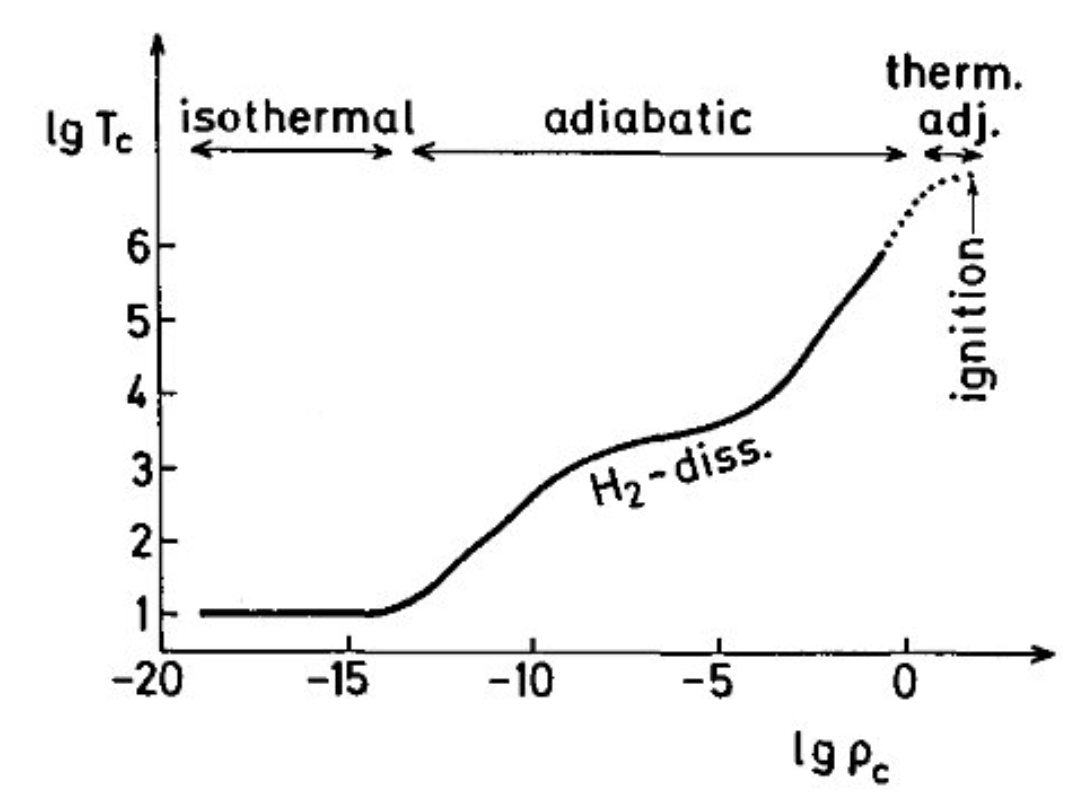
\includegraphics[width=10cm]{figures/Tvsrho_protostars}}
\end{figure}

{\noindent}\textbf{Deuterium ignition and convection:} In Figure \ref{fig:RvsMprotostars}, the next evolutionary phase begins at $0.25\,{\rm M_\odot}$, and continues to $0.7\,{\rm M_\odot}$. This stage is marked by two distinct but interrelated phenomena: the onset of nuclear burning and the onset of convection. The driving force behind both phenomena is that, as the protostar gains mass, its interior temperature rises. For a polytrope, which is not an unreasonable description of the accreting protostar, the central temperature rises with mass to the $T_c\propto M^{(2\gamma-2)/(3\gamma-2)}$. Thus even at fixed entropy the central temperature must rise as the star gains mass.

{\noindent}Once $T_c$ reaches $\sim10^6\,{\rm K}$, deuterium will ignite at the center of the protostar. This generally happens at a mass of hundredths to tenths of ${\rm M_\odot}$, depending on the choice of accretion rate and boundary condition. This has two significant effects. The first is that deuterium acts as a thermostat for the star's center, much as hydrogen does
in a main sequence star. Because the energy generation rate is so incredibly sensitive to $T$, any slight raise in the temperature causes it to jump enough to raise the pressure and adiabatically expand the star, reducing $T$. Thus, $T_c$ becomes fixed at $10^6\,{\rm K}$. The star adjusts its radius accordingly, which generally requires that the radius increase to keep $T_c$ nearly constant as the mass rises. Thus deuterium burning temporarily halts core contraction. Both effects are visible in Figure \ref{fig:RvsMprotostars}. The halting of core contraction is apparent from the way the dotted lines showing constant mass enclosed bend upward at $\sim0.3\,{\rm M}$, and the nearly constant core temperature is visible from the fact that, between
$\sim0.25\,{\rm M}$ and $3-4\,{\rm M}$, a factor of more than $10$ in mass, the central temperature stays within a factor of $2$ of $10^6\,{\rm K}$.

{\noindent}The second effect of deuterium burning that it causes a rapid rise in the entropy at the center of the star. This has the effect of starting up convection in the star. Before deuterium burning the star is generally stable against convection. That is because the entropy profile is determined by infall, and since shells that fall onto the star later arrive at higher velocities (due to the rising $M_*$), they have higher entropy. Thus $s$ is an increasing function of $M_r$, which is the condition for convective stability. Deuterium burning reverses this, and convection follows, eventually turning much of the star convective. This also ensures the star a continuing supply of deuterium fuel, since convection will drag gas from the outer parts of the star down to the core, where they can be burned.

{\noindent}An important caveat here is that, although D burning encourages convection, it is not necessary for it. In the absence of D, or for very high accretion rates, the onset of convection is driven by the increasing luminosity of the stellar core as it undergoes KH contraction. This energy must be transported outwards, and as the star's mass rises and the luminosity goes up, eventually the energy that must be transported exceeds the ability of radiation to carry it. Convection results. For very high accretion rates, this effect drives the onset of convection even before the onset of D burning.

{\noindent}A third effect of the deuterium thermostat is that it forces the star to obey a nearly-linear mass-radius relation, and thus to obey a particular relationship between accretion rate and accretion luminosity. One can show that for a polytrope the central temperature and surface escape speed are related by

\begin{align*}
    \psi = \frac{GM}{R} = \frac{1}{2} v_{\rm esc}^2 = T_n \frac{k_BT_c}{\mu m_{\rm H}} ~ [{\rm erg\,g^{-1}}]
\end{align*}

{\noindent}where $T_c$ is the core temperature, $T_n$ is a dimensionless constant of order unity that depends only on the polytropic index, and $\mu$ is the mean mass per particle in units of hydrogen masses. For $n=3/2$, expected for a fully convective star, $T_n=1.86$. Plugging in this value of $T_n$, $\mu=0.61$ (the mean molecular weight for a fully ionized gas of H and He in the standard abundance ratio), and $T_c=10^6\,{\rm K}$, one obtains $\psi=2.5\times10^{14}\,{\rm erg\,g^{-1}}$ as the energy yield from accretion.

{\noindent}\textbf{Deuterium exhaustion and formation of a radiative barrier:} The next evolutionary phase, which runs from $0.6-3\,{\rm M_\odot}$ in Figure \ref{fig:RvsMprotostars}, is marked by the exhaustion of deuterium in the stellar core. Deuterium can only hold up the star for a finite amount of time. The reason is simply that there isn't that much of it. Each deuterium burned provides $5.5\,{\rm MeV}$ of energy, comparable the $7\,{\rm MeV}$ per hydrogen provided by burning hydrogen, but there are only $2\times10^{-5}$ D nuclei per H nuclei. Thus, at fixed luminosity the ``main sequence'' lifetime for D burning is shorter than that for H burning by a factor of $2\times10^{-5}\times5.5/7 = 1.6\times10^{-5}$.

{\noindent}We therefore see that, while a main sequence star can burn hydrogen for $10^{10}\,{\rm yr}$, a comparable pre-main sequence star of the same mass and luminosity burning deuterium can only do it for only a few times $10^5\,{\rm yr}$. To be more precise, the time required for a star to exhaust its deuterium is

\begin{align*}
    t_{\rm D} = \frac{[{\rm D/H}]\Delta E_DM_*}{m_{\rm H}L_*} = 1.5\times10^6 [{\rm yr\,M_*L_{*,0}^{-1}}].
\end{align*}

{\noindent}Thus deuterium burning will briefly hold up a star's contraction, but cannot delay it for long. However, a brief note is in order here: while this delay is not long compared to the lifetime of a star, it is comparable to the formation time of the star. Recall that typical accretion rates are of order a few times $10^{-6}\,{M_\odot\,yr^{-1}}$, so a $1\,{\rm M_\odot}$ star takes a few times $10^5\,{\rm yr}$ to form. Thus stars may burn deuterium for most of the time they are accreting.

{\noindent}The exhaustion of deuterium does not mean the end of deuterium burning, since fresh deuterium that is brought to the star as it continues accreting will still burn. Instead, the exhaustion of core deuterium happens for a more subtle reason. As the deuterium supply begins to run out, the rate of energy generation in the core becomes insufficient to prevent it from undergoing further contraction, leading to rising temperatures. The rise in central temperature lowers the opacity, which is govern by Kramers' law: $\kappa\propto\rho T^{-3.5}$. This in turn makes it easier for radiation to transport energy outward. Eventually this shuts off convection somewhere within the star, leading to formation of what is called a \textbf{radiative barrier}.

{\noindent}The formation of the barrier ends the transport of D to the stellar center. The tiny bit of D left in the core is quickly consumed, and, without D burning to drive an entropy gradient, convection shuts off through the entire core. This is the physics behind the nearly-simultaneous end of central D burning and central convection that occurs near $0.6\,{\rm M}$ in Figure \ref{fig:RvsMprotostars}. After this transition, the core is able to resume contraction, and D continues to burn as fast as it accretes. However, it now does so in a shell around the core rather than in the core.

{\noindent}\textbf{Swelling:} The next evolutionary phase, which occurs from $3-4\,{\rm M}$ in Figure \ref{fig:RvsMprotostars}, is swelling. This phase is marked by a marked increase in the star's radius over a relative short period of time. The physical mechanism driving this is the radiative barrier discussed above. The radiative barrier forms because increasing temperatures drive decreasing opacities, allowing more rapid transport of energy by radiation. The decreased opacity allows the center of the star to lose entropy rapidly, and the entropy to be transported to the outer parts of the star via radiation. The result is a wave of luminosity and entropy that propagates outward through the star.

\begin{figure}[t]
    \floatbox[{\capbeside\thisfloatsetup{capbesideposition={right,top},capbesidewidth=4cm}}]{figure}[\FBwidth]
    {\caption{\footnotesize{Radius versus mass (top) and maximum temperature versus mass (bottom) for protostars accretting at different rates. The accretion rate is indicated by the line style, as illustrated in the top panel. For each accretion rate there are two lines, one thick and one thin. The thick line is for the observed Milky Way deuterium abundance, while the thin line is the result assuming zero deuterium abundance. Figure taken from Krumholtz (2015).}}
    \label{fig:swelling}}
    {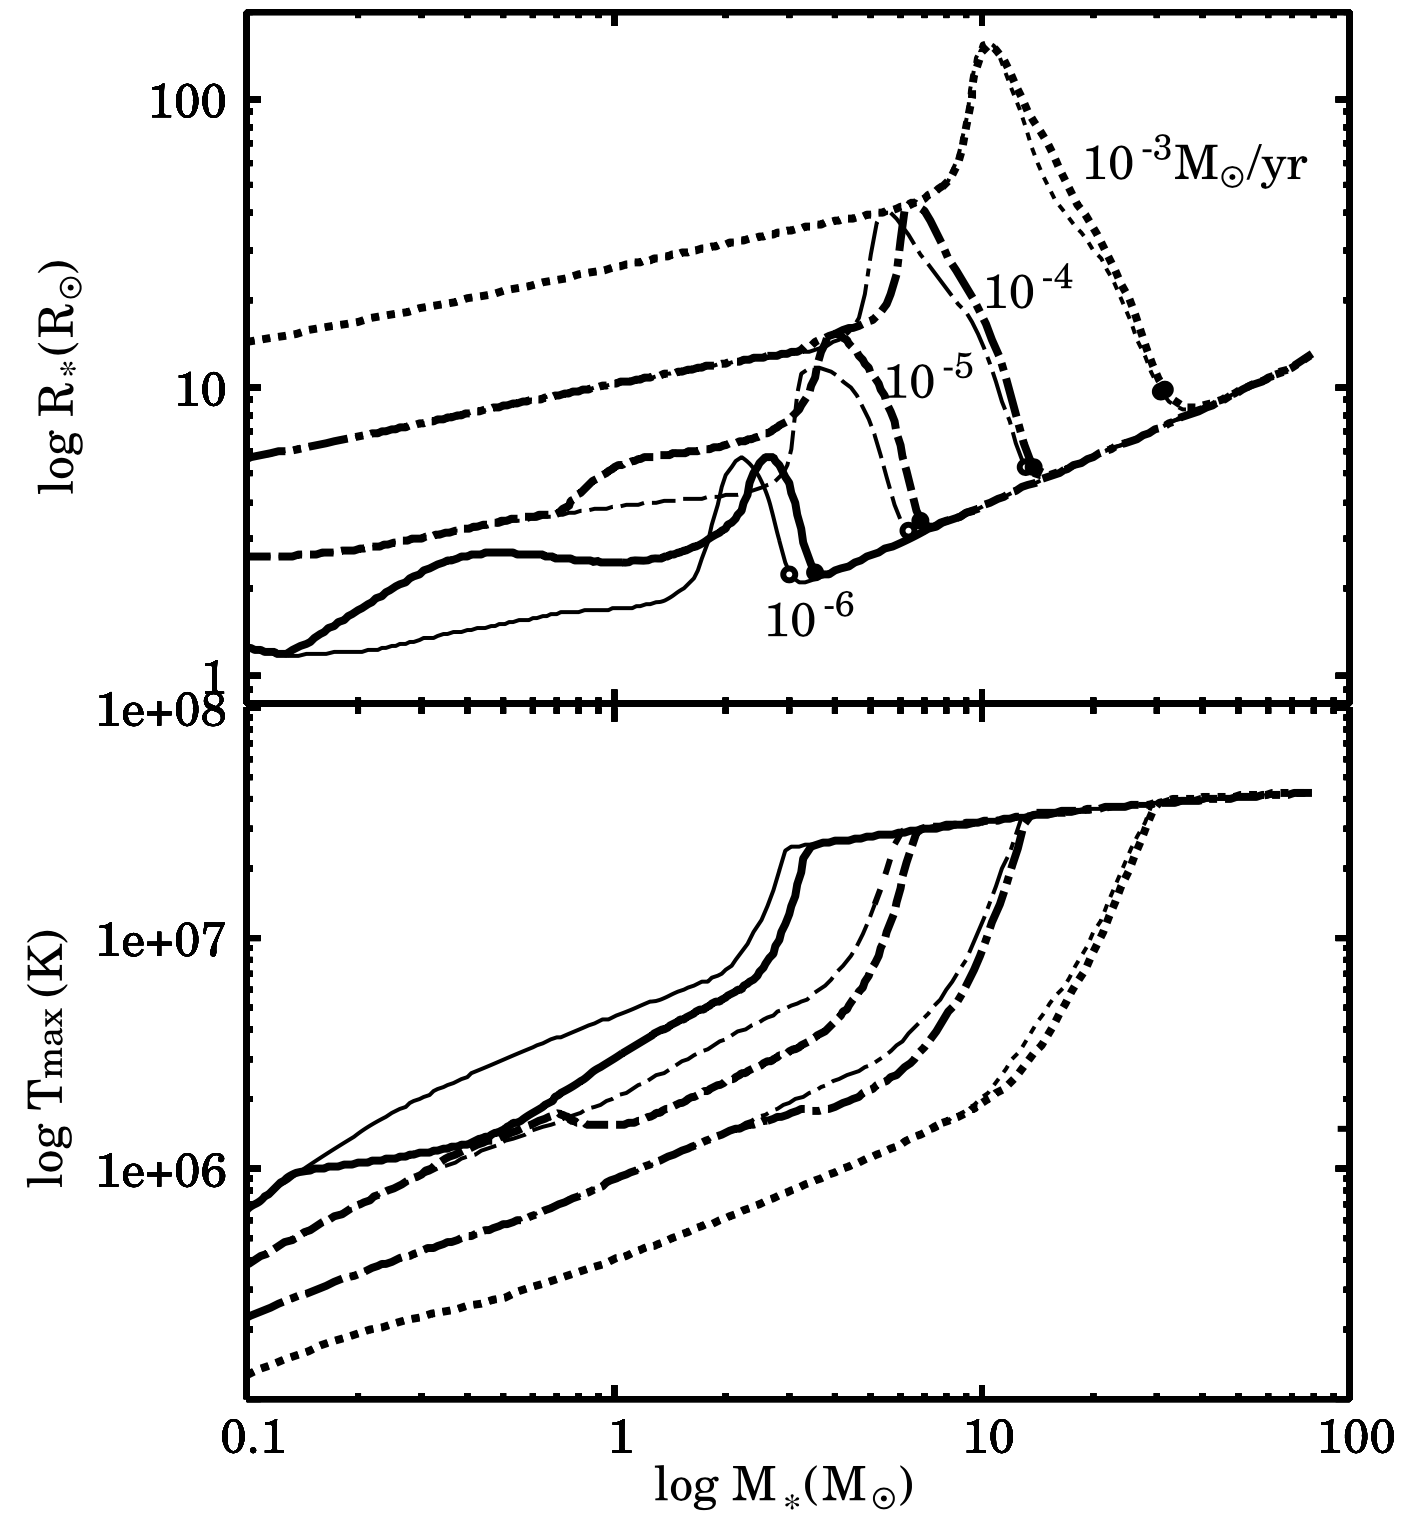
\includegraphics[width=10cm]{figures/swelling.png}}
\end{figure}

{\noindent}Once the wave of luminosity and entropy gets near the stellar surface, which is not confined by the weight of overlying material, the surface undergoes a rapid expansion, leading to rapid swelling. The maximum radius, and the mass at which the swelling phase occurs, is a strong function of the accretion rate (Figure \ref{fig:swelling}). However, even at very low accretion rates, swelling does not occur until the mass exceeds $1\,{\rm M_\odot}$.

{\noindent}\textbf{Contraction to the Main Sequence:} The final stage of protostellar evolution is contraction to the main sequence. Once the entropy wave hits the surface, the star is able to begin losing energy and entropy fairly quickly, and it resumes contraction. This marks the final phase of protostellar evolution, visible above $\sim4\,{\rm M_\odot}$ in Figure \ref{fig:RvsMprotostars}. Contraction ends once the core temperature becomes hot enough to ignite hydrogen, landing the star at least on the main sequence.

{\noindent}\textbf{Observable evolution of protostars:} We have just discussed the interior behaviour of an evolving protostar. While this is important, it is also critical to predict the observable properties of the star during this evolutionary sequence. In particular, we wish to understand the star's luminosity and effective temperature, which dictate its location on the HR diagram. The required values can simply be read off from the evolutionary models (Figure \ref{fig:HRmodels}), giving rise to a track of luminosity versus effective temperature in the HR diagram.

\begin{figure}[t]
    \floatbox[{\capbeside\thisfloatsetup{capbesideposition={right,top},capbesidewidth=4cm}}]{figure}[\FBwidth]
    {\caption{\footnotesize{Solid lines show tracks taken by stars of varying masses from $0.1\,{\rm M_\odot}$ (rightmost line) to $7\,{\rm M_\odot}$ (leftmost line) in the theoretical HR diagram of luminosity versus effective temperature. Stars begin at the upper right of the tracks and evolve to the lower left; tracks end at the main sequence. Dashed lines represent isochrones corresponding to $10^6$, $10^7$, and $10^8$ years from top right to bottom left. Figure taken from Krumholtz (2015).}}
    \label{fig:HRmodels}}
    {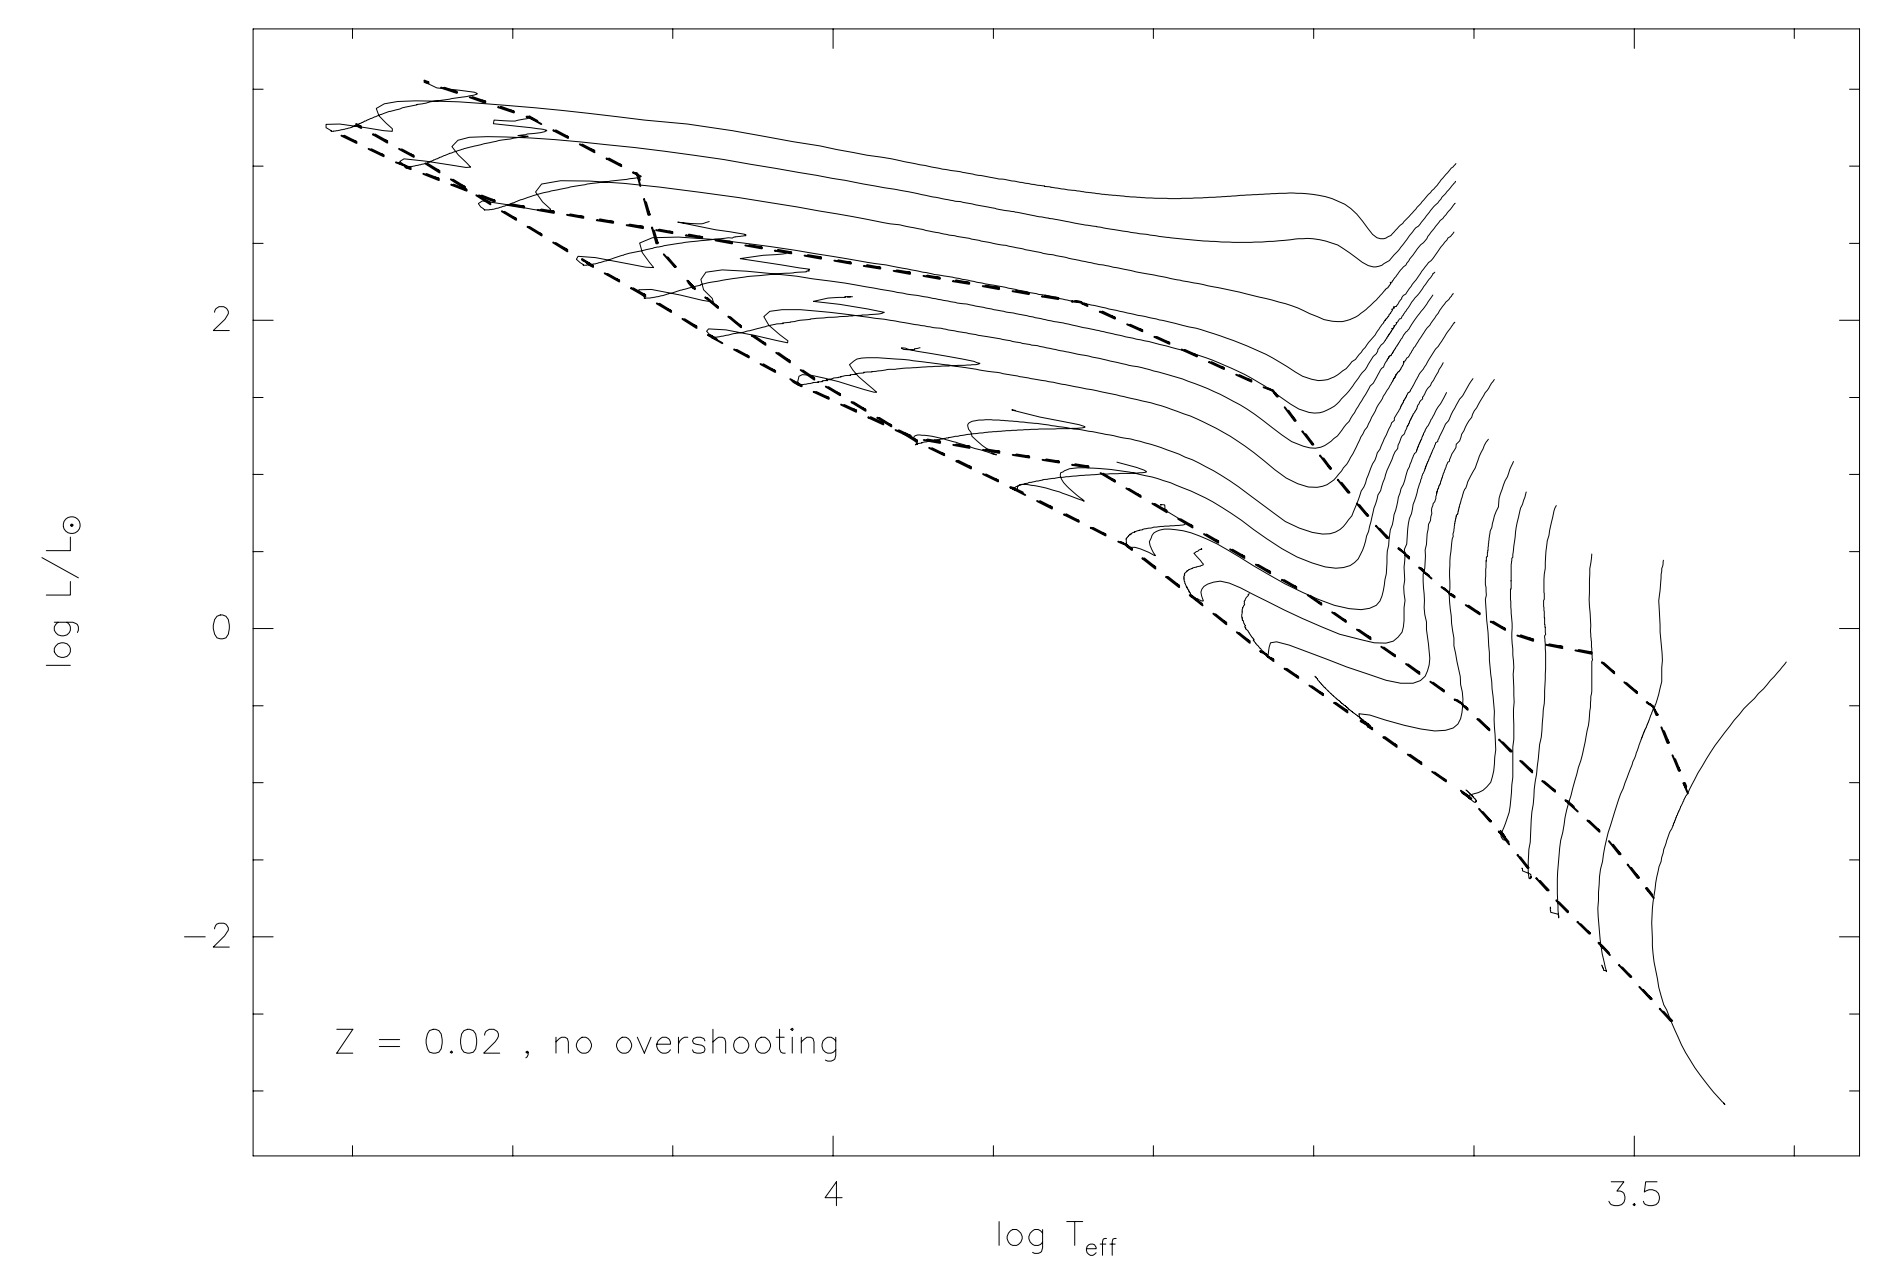
\includegraphics[width=10cm]{figures/HR_models.png}}
\end{figure}

{\noindent}\textbf{The birthline:} Before delving into the tracks themselves, we have to ask what is actually observable. As long as a star is accreting from its parent core, it will probably not be visible in the optical, due to the high opacity of the dusty gas in the core. Thus we are most concerned with stars' appearance in the HR diagram only after they have finished their main accretion phase. We refer to stars that are still accreting and thus not generally optically-observable as \textbf{protostars}, and those that are in this post-accretion phase as \textbf{pre-main sequence stars}.

{\noindent}For stars below $1\,{\rm M}$, examining Figure \ref{fig:RvsMprotostars}, we see that the transition from protostar to pre-main sequence star will occur some time after the onset of deuterium burning, either during the core or shell burning phases depending on the mass and accretion history. More massive stars will become visible only during KH contraction, or even after the onset of hydrogen burning. The lowest mass stars might be observable even before the start of deuterium burning. However, for the majority of the pre-main sequence stars that we can observe, they first become visible during the D burning phase.

{\noindent}Since there is a strict mass-radius relation during core deuterium burning (with some variation due to varying accretion rates), there must be a corresponding relationship between $L$ and $T$, just like the main sequence. We call this line in the HR diagram, on which protostars first appear, the \textbf{birthline}; see Figure \ref{fig:birthline}. Since young stars are larger and more luminous that main sequence stars of the same mass, this line lies at higher $L$ and lower $T$ than the main sequence.

{\noindent}\textbf{The Hayashi track:} Now that we understand what is observable, let us turn to the tracks themselves. The tracks shown in Figures \ref{fig:HRmodels} and \ref{fig:birthline} show several distinct features. One is that, for low mass stars, the initial phases of evolution in the HR diagram are nearly vertically, i.e., at constant $T_{\rm eff}$. The vertical tracks for different masses are very close together. This vertical part of the evolution is called the \textbf{Hayashi track}, after its discoverer, who predicted it theoretically (Hayashi, 1961). For low mass stars, the majority of the Hayashi track lies after the birthline, so it is directly observable.

\begin{figure}[t]
    \floatbox[{\capbeside\thisfloatsetup{capbesideposition={right,top},capbesidewidth=4cm}}]{figure}[\FBwidth]
    {\caption{\footnotesize{Thin lines show tracks taken by stars of varying masses (indicated by the annotation, in ${\rm M_\odot}$) in the theoretical HR diagram of luminosity versus effective temperature. Stars begin at the upper right of the tracks and evolve to the lower left; tracks end at the main sequence. The thick line crossing the tracks is the birthline, the point at which the stars stop accreting and become optically visible. Squares and circles represent the properties of observed young stars. Figure adapted from from Palla \& Stahler (1990). Figure taken from Krumholtz (2015).}}
    \label{fig:birthline}}
    {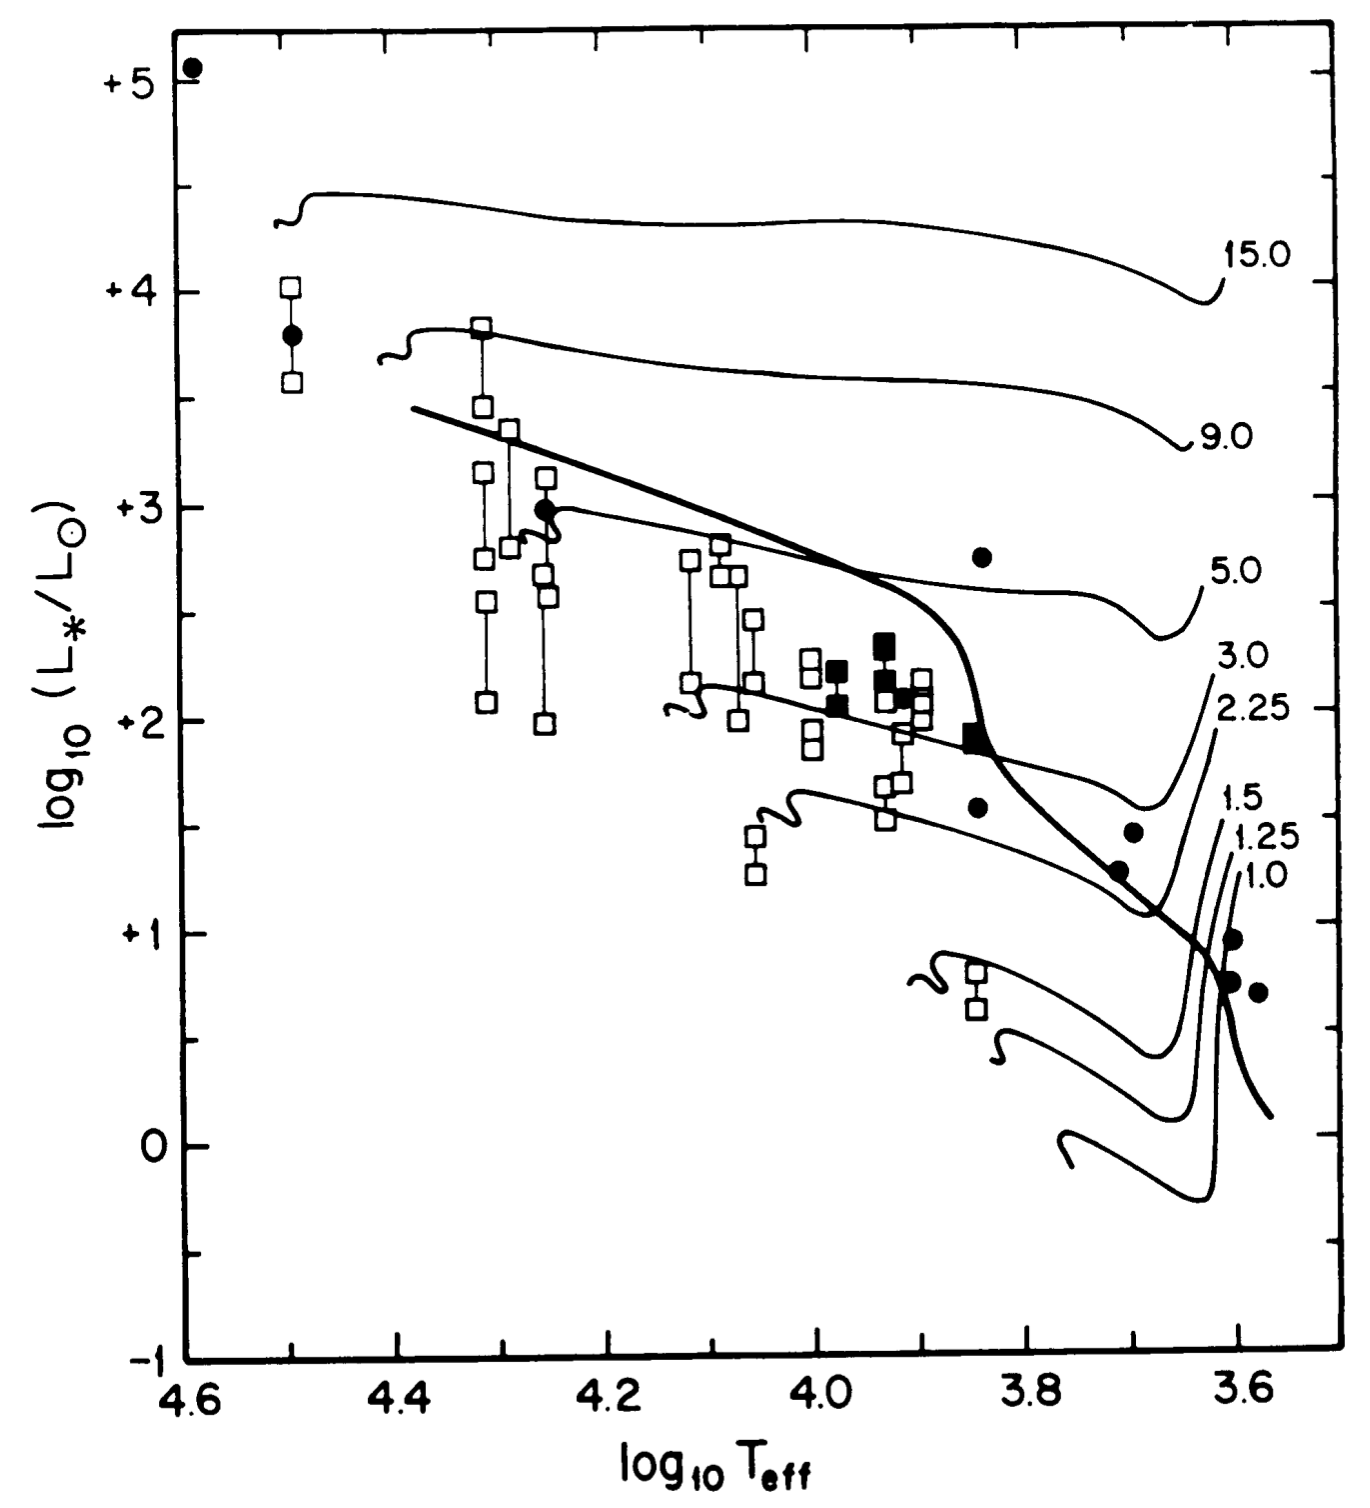
\includegraphics[width=8cm]{figures/birthline.png}}
\end{figure}

{\noindent}The origin of the Hayashi track is in the physics of opacity in stellar atmospheres at low temperature. At temperatures below about $10^4\,{\rm K}$, hydrogen becomes neutral, and the only free electrons available come from metal atoms with lower ionization energies. Some of these electrons become bound with hydrogen atoms, forming H$^-$, and this ion is the dominant source of opacity. Thus the opacity depends on the number of free electrons provided by metal atoms, which in turn depends extremely sensitively on the temperature.

{\noindent}If the temperature falls too low, the opacity will be so low that, even integrating through the rest of the star's mass, the optical depth to infinity will be $<2/3$. Since the photosphere must always be defined by a surface of optical depth unity, this effectively establishes a minimum surface temperature for the star required to maintain $\tau\sim1$. This minimum temperature depends weakly on the star's mass and radius, but to good approximation it is simply $T_{\rm min}=T_H=3500\,{\rm K}$, where $T_H$ is the \textbf{Hayashi temperature}. Low mass protostars, due to their large radii, wind up right against this limit, which is why they all contract along vertical tracks that are packed close together in $T_{\rm eff}$.

{\noindent}\textbf{The Heyney track:} Contraction at nearly constant $T_{\rm eff}$ continues until the star contracts enough to raise its surface temperature above $T_H$. This increase in temperature also causes the star to transition from convective to radiative, since the opacity drops with temperature at high temperatures, and a lower opacity lets radiation rather than convection carry the energy outward.

{\noindent}In the HR diagram, the contraction and increase in $T_{\rm eff}$ produces a vaguely horizontal evolutionary track. This is called the \textbf{Heyney track}. The star continues to contract until its center becomes warm enough to allow H burning to begin. At that point it may contract a small additional amount, but the star is essentially on the main sequence. The total time required depends on the stellar mass, but it ranges from several hundred ${\rm Myr}$ for $0.1\,{\rm M_\odot}$ stars to essentially zero time for very massive stars, which reach the main sequence while still accreting.

\subsubsection{Follow-up Questions}

\begin{itemize}
    \item How do you calculate the Jeans mass?
    \item What happens to the temperature during adiabatic contraction?
    \item Draw a plot of density versus temperature to distinguish between the contracting and collapsing phases.
\end{itemize}

% --------------------------------------------------------------
%               14. 
% --------------------------------------------------------------

\newpage
\subsection{Question 14}

Sketch the rotation curve for a typical spiral galaxy. Show that a flat rotation curve implies the existence of a dark matter halo with a density profile that drops off as $1/r^2$.

\subsubsection{Short answer}

\begin{figure}[h]
    \floatbox[{\capbeside\thisfloatsetup{capbesideposition={right,top},capbesidewidth=4cm}}]{figure}[\FBwidth]
    {\caption{\footnotesize{Rotation curve of the Milky Way. Inside the ``Solar circle'', that is at $R<R_0$, the radial velocity is determined quite accurately using the tangent point method; the measurements outside have larger uncertainties. Source: D. Clemens 1985, Massachusetts-Stony Brook Galactic plane CO survey - The Galactic disk rotation curve ApJ 295, 422, p.429, Fig. 3. Figure taken from Schneider (2015).}}
    \label{fig:rotationcurve}}
    {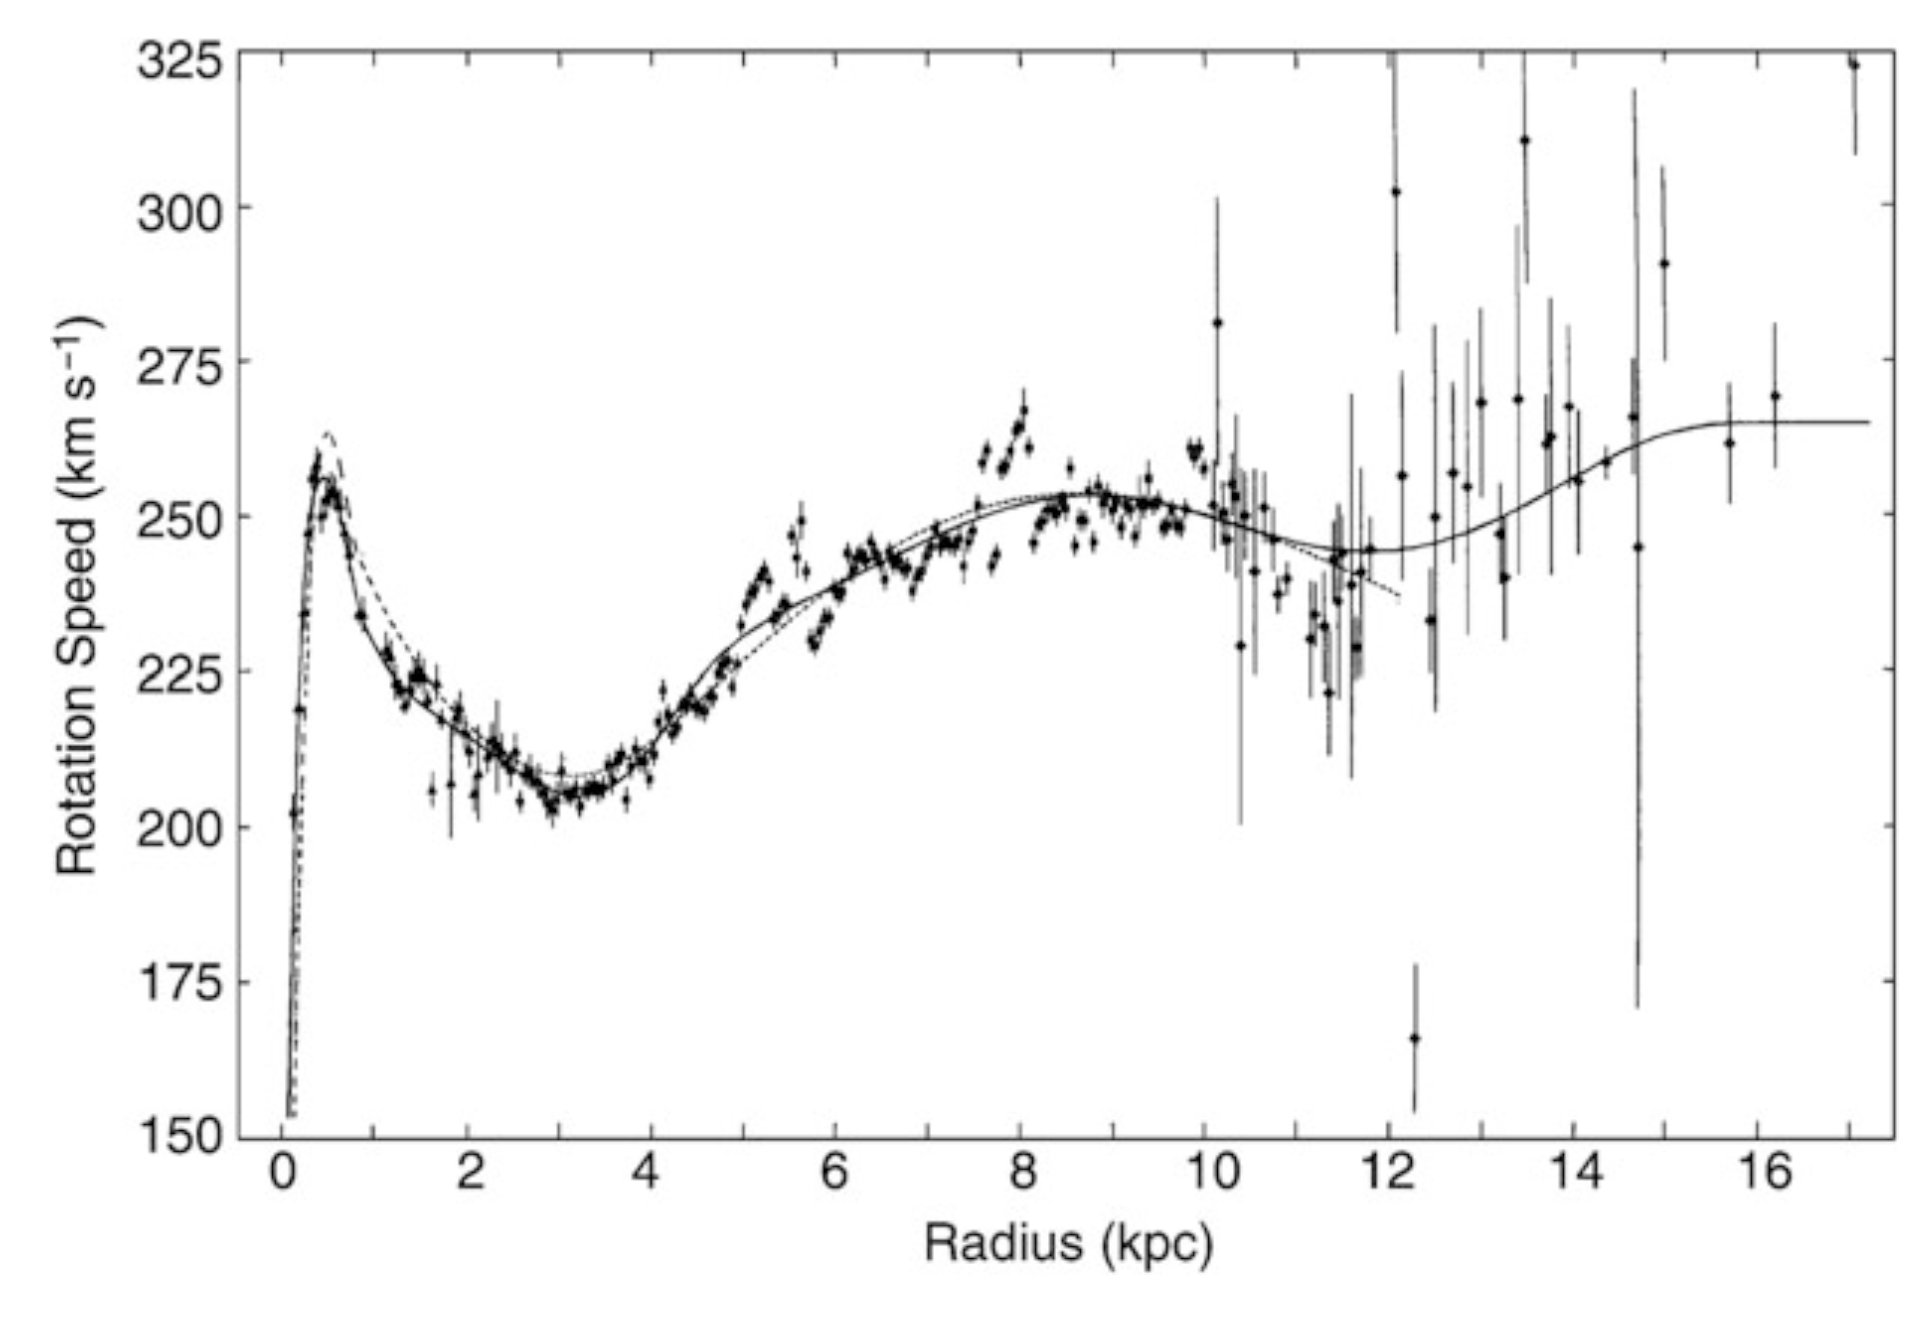
\includegraphics[width=10cm]{figures/RotationCurve.png}}
\end{figure}

\subsubsection{Additional context}

From observations of the velocity of stars or gas around the Galactic center, the rotational velocity $V$ can be determined as a function of the distance $R$ from the Galactic center.

{\noindent}\textbf{Decomposition of rotational velocity:} We consider an object at distance $R$ from the Galactic center which moves along a circular orbit in the Galactic plane, has a distance $D$ from the Sun, and is located at a Galactic longitude $\ell$ (see Figure \ref{fig:differentialrotation}). In a Cartesian coordinate system with the Galactic center at the origin, the positional and velocity vectors (we only consider the two components in the Galactic plane because we assume a motion in the plane) are given by

\begin{align*}
    \mathbf{r} = R\left(\frac{\sin\theta}{\cos\theta}\right) ~ [{\rm kpc}], ~~~ \mathbf{V} = \mathbf{\dot{r}} = V(R)\left(\frac{\cos\theta}{-\sin\theta}\right) ~ [{\rm km\,s^{-1}}],
\end{align*}

{\noindent}where $\theta$ denotes the angle between the Sun and the object as seen from the Galactic center. From the geometry shown in Figure \ref{fig:differentialrotation} it follows that

\begin{align*}
    \mathbf{r} = \left(\frac{D\sin\ell}{R_0-D\cos\ell}\right) ~ [{\rm kpc}].
\end{align*}

{\noindent}If we now identify the two expressions for the components of $\mathbf{r}$, we obtain

\begin{align*}
    \sin\theta=\left(\frac{D}{R}\right)\sin\ell ~ [{\rm dimensionless}], ~~~ \cos\theta=\left(\frac{R_0}{R}\right) - \left(\frac{D}{R}\right)\cos\ell ~ [{\rm dimensionless}].
\end{align*}

{\noindent}If we disregard the difference between the velocities of the Sun and the LSR we get $\mathbf{V}_\odot\approx\mathbf{V} = (V_0,0)$ in this coordinate system. Thus the relative velocity between the object and the Sun is, in Cartesian coordinates,

\begin{align*}
    \Delta\mathbf{V} = \mathbf{V}-\mathbf{V}_\odot = \left(\frac{V\left(\frac{R_0}{R}\right) - V\left(\frac{D}{R}\right)\cos\ell - V_0}{-V\left(\frac{D}{R}\right)\sin\ell}\right) ~ [{\rm km\,s^{-1}}].
\end{align*}

{\noindent}With the angular velocity defined as

\begin{align*}
    \Omega \equiv \frac{V(R)}{R} ~ [{\rm rad\,s^{-1}}]
\end{align*}

{\noindent}we obtain for the relative velocity

\begin{align*}
    \Delta\mathbf{V} = \left(\frac{R(\Omega-\Omega_0) - \Omega D\cos\ell}{-D\Omega\sin\ell}\right) ~ [{\rm km\,s^{-1}}],
\end{align*}

\begin{figure}[t]
    \floatbox[{\capbeside\thisfloatsetup{capbesideposition={right,top},capbesidewidth=5cm}}]{figure}[\FBwidth]
    {\caption{\footnotesize{Geometric derivation of the formalism of differential rotation:\\
    $v_r=v_r^*-v_r^\odot=v_*\sin\ell^*-v_\odot\sin\ell$, \\
    $v_t = v_t^*-v_t^\odot=v_*\cos\ell^*-v_\odot\cos\ell$. \\
    One has: \\
    $\frac{\sin\ell}{R}=\frac{\sin(\pi-\ell^*)}{R_0}=\frac{\sin\ell^*}{R_0}$, \\
    $R\cos\ell^*+D=R_0\cos\ell$, \\
    which implies\\
    $v_r=R_0 \left(\frac{v_*}{R}-\frac{v_\odot}{R_0}\right) \sin\ell$ \\
    $=(\Omega-\Omega_0)R_0\sin\ell$, \\ 
    $v_t=R_0 \left(\frac{v_*}{R}-\frac{v_\odot}{R_0}\right) \cos\ell -D\frac{v_*}{R}$ \\
    $=(\Omega-\Omega_0)R_0\cos\ell -\Omega D$. \\
    Figure taken from Schneider (2015).}}
    \label{fig:differentialrotation}}
    {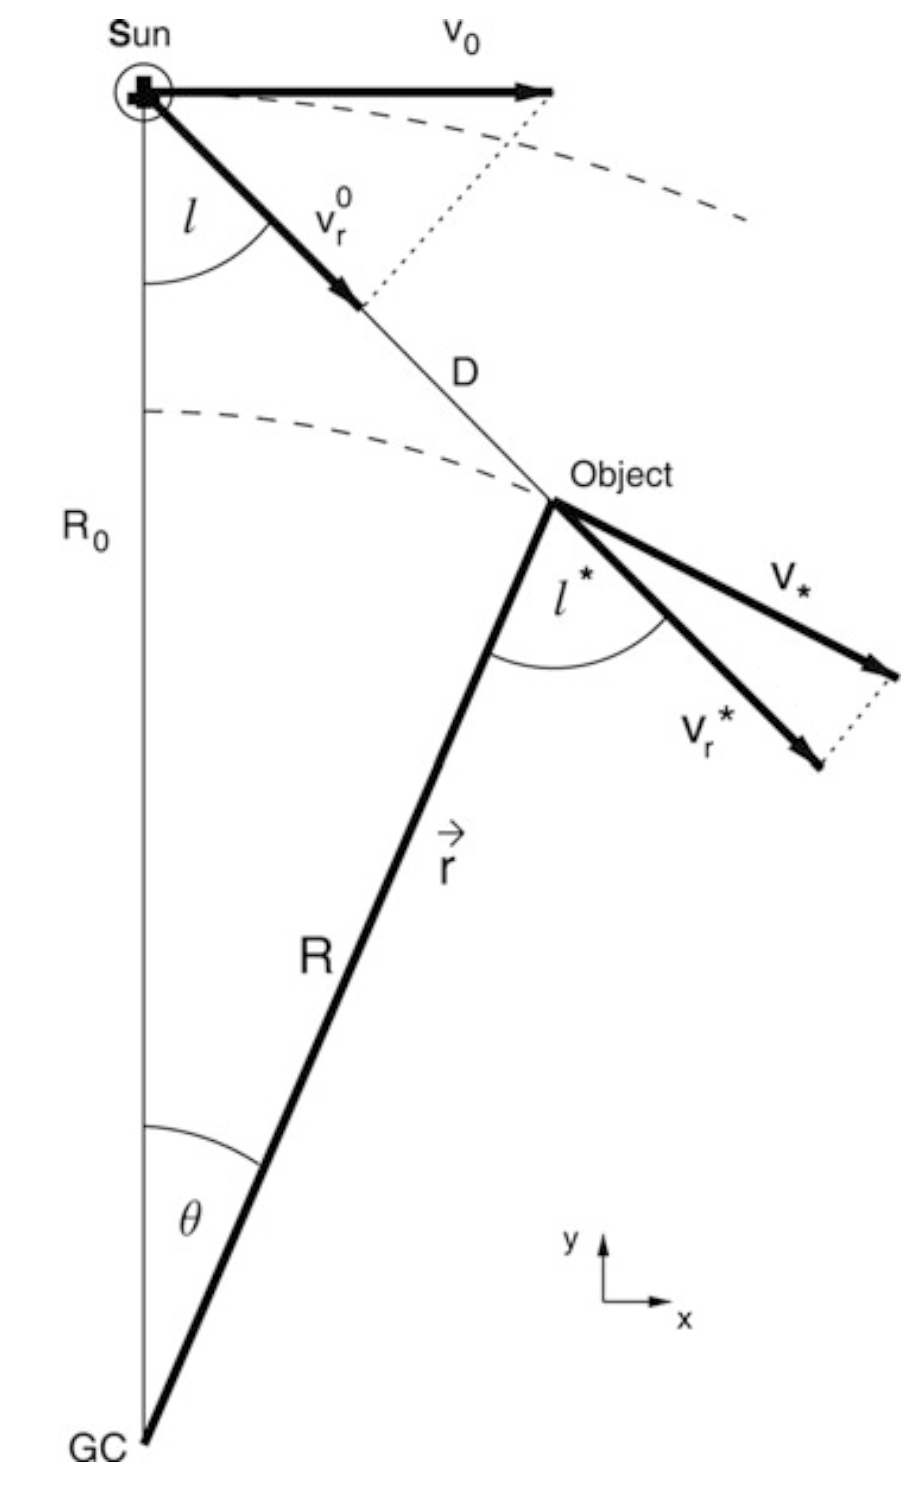
\includegraphics[width=8cm]{figures/DifferentialRotation.png}}
\end{figure}

{\noindent}where $\Omega_0=V_0/R_0$ is the angular velocity of the Sun. The radial and tangential velocities of this relative motion then follow by projection of $\Delta\mathbf{V}$ along the direction parallel or perpendicular, respectively, to the separation vector,

\begin{align*}
    v_r &= \Delta\mathbf{V}\cdot\left(\frac{\sin\ell}{-\cos\ell}\right) = (\Omega-\Omega_0)R_0\sin\ell ~ [{\rm km\,s^{-1}}], \\
    v_t &= \Delta\mathbf{V}\cdot\left(\frac{\cos\ell}{\sin\ell}\right) = (\Omega-\Omega_0)R_0\cos\ell - \Omega D ~ [{\rm km\,s^{-1}}].
\end{align*}

{\noindent}A purely geometric derivation of these relations is given in Figure \ref{fig:differentialrotation}.

{\noindent}\textbf{Rotation curve near $R_0$, Oort constants:} One can derive the angular velocity by means of measuring $v_r$ from the equation above, but not the radius $R$ to which it corresponds. Therefore, by measuring the radial velocity alone, $\Omega(R)$ cannot be determined. If one measures $v_r$ and, in addition, the proper motion $\mu=v_t/D$ of stars, then $\Omega$ and $D$ can be determined from the equations above, and from $D$ and $\ell$ one obtains $R=\sqrt{R_0^2+D^2-2R_0D\cos\ell}$. The effects of extinction prohibits the use of this method for large distances $D$, since we have considered objects in the Galactic disk. For small distances $D\ll R_0$, which implies $\lvert R-R_0\rvert\ll R_0$, we can make a local approximation by evaluating the expressions above only up to first order in $(R-R_0)/R_0$. In this linear approximation we get

\begin{align*}
    \Omega-\Omega_0\approx \left(\frac{{\rm d}\Omega}{{\rm d}R}\right)_{R_0} (R-R_0) ~ [{\rm km\,s^{-1}\,kpc^{-1}}],
\end{align*}

{\noindent}where the derivative has to be evaluated at $R=R_0$. Hence

\begin{align*}
    v_r = (R-R_0) \left(\frac{{\rm d}\Omega}{{\rm d}R}\right)_{R_0} R_0\sin\ell ~ [{\rm km\,s^{-1}}],
\end{align*}

{\noindent}and furthermore, with the definition of angular velocity $\Omega(R)$,

\begin{align*}
    R_0\left(\frac{{\rm d}\Omega}{{\rm d}R}\right)_{R_0} = \frac{R_0}{R} \left[\left(\frac{{\rm d}V}{{\rm d}R}\right)_{R_0} - \frac{V}{R}\right] \approx \left(\frac{{\rm d}V}{{\rm d}R}\right)_{R_0} - \frac{V_0}{R_0} ~ [{\rm km\,s^{-1}\,kpc^{-1}}],
\end{align*}

{\noindent}in zeroth order in $(R-R_0)/R_0$. Combining the last two equations yield

\begin{align*}
    v_r = \left[\left(\frac{{\rm d}V}{{\rm d}R}\right)_{R_0} - \frac{V_0}{R_0}\right] (R-R_0)\sin\ell ~ [{\rm km\,s^{-1}}],
\end{align*}

{\noindent}in analogy to this, we obtain for the tangential velocity

\begin{align*}
    v_t = \left[\left(\frac{{\rm d}V}{{\rm d}R}\right)_{R_0} - \frac{V_0}{R_0}\right] (R-R_0)\cos\ell - \Omega_0D ~ [{\rm km\,s^{-1}}].
\end{align*}

{\noindent}For $\lvert R-R_0\rvert\ll R_0$ it follows that $(R_0-R)\approx D\cos\ell$; if we insert this into $v_r$ and $v_t$ we get

\begin{align*}
    v_r \approx AD\sin2\ell ~ [{\rm km\,s^{-1}}], ~~~ v_t \approx AD\cos2\ell+BD ~ [{\rm km\,s^{-1}}],
\end{align*}

{\noindent}where $A$ and $B$ are the \textbf{Oort constants}:

\begin{align*}
    A \equiv -\frac{1}{2} \left[\left(\frac{{\rm d}V}{{\rm d}R}\right)_{R_0} -\frac{V_0}{R_0}\right] ~ [{\rm km\,s^{-1}\,kpc^{-1}}],\\
    B \equiv -\frac{1}{2} \left[\left(\frac{{\rm d}V}{{\rm d}R}\right)_{R_0} +\frac{V_0}{R_0}\right] ~ [{\rm km\,s^{-1}\,kpc^{-1}}].
\end{align*}

\begin{figure}[t]
    \floatbox[{\capbeside\thisfloatsetup{capbesideposition={right,top},capbesidewidth=4cm}}]{figure}[\FBwidth]
    {\caption{\footnotesize{The radial velocity $v_r$ of stars at a fixed distance $D$ is proportional to $\sin2\ell$; the tangential velocity $v_t$ is a linear function of $\cos2\ell$. From the amplitude of the oscillating curves and from the mean value of $v_t$ the Oort constants $A$ and $B$ can be derived. Figure taken from Schneider (2015).}}
    \label{fig:vtvr}}
    {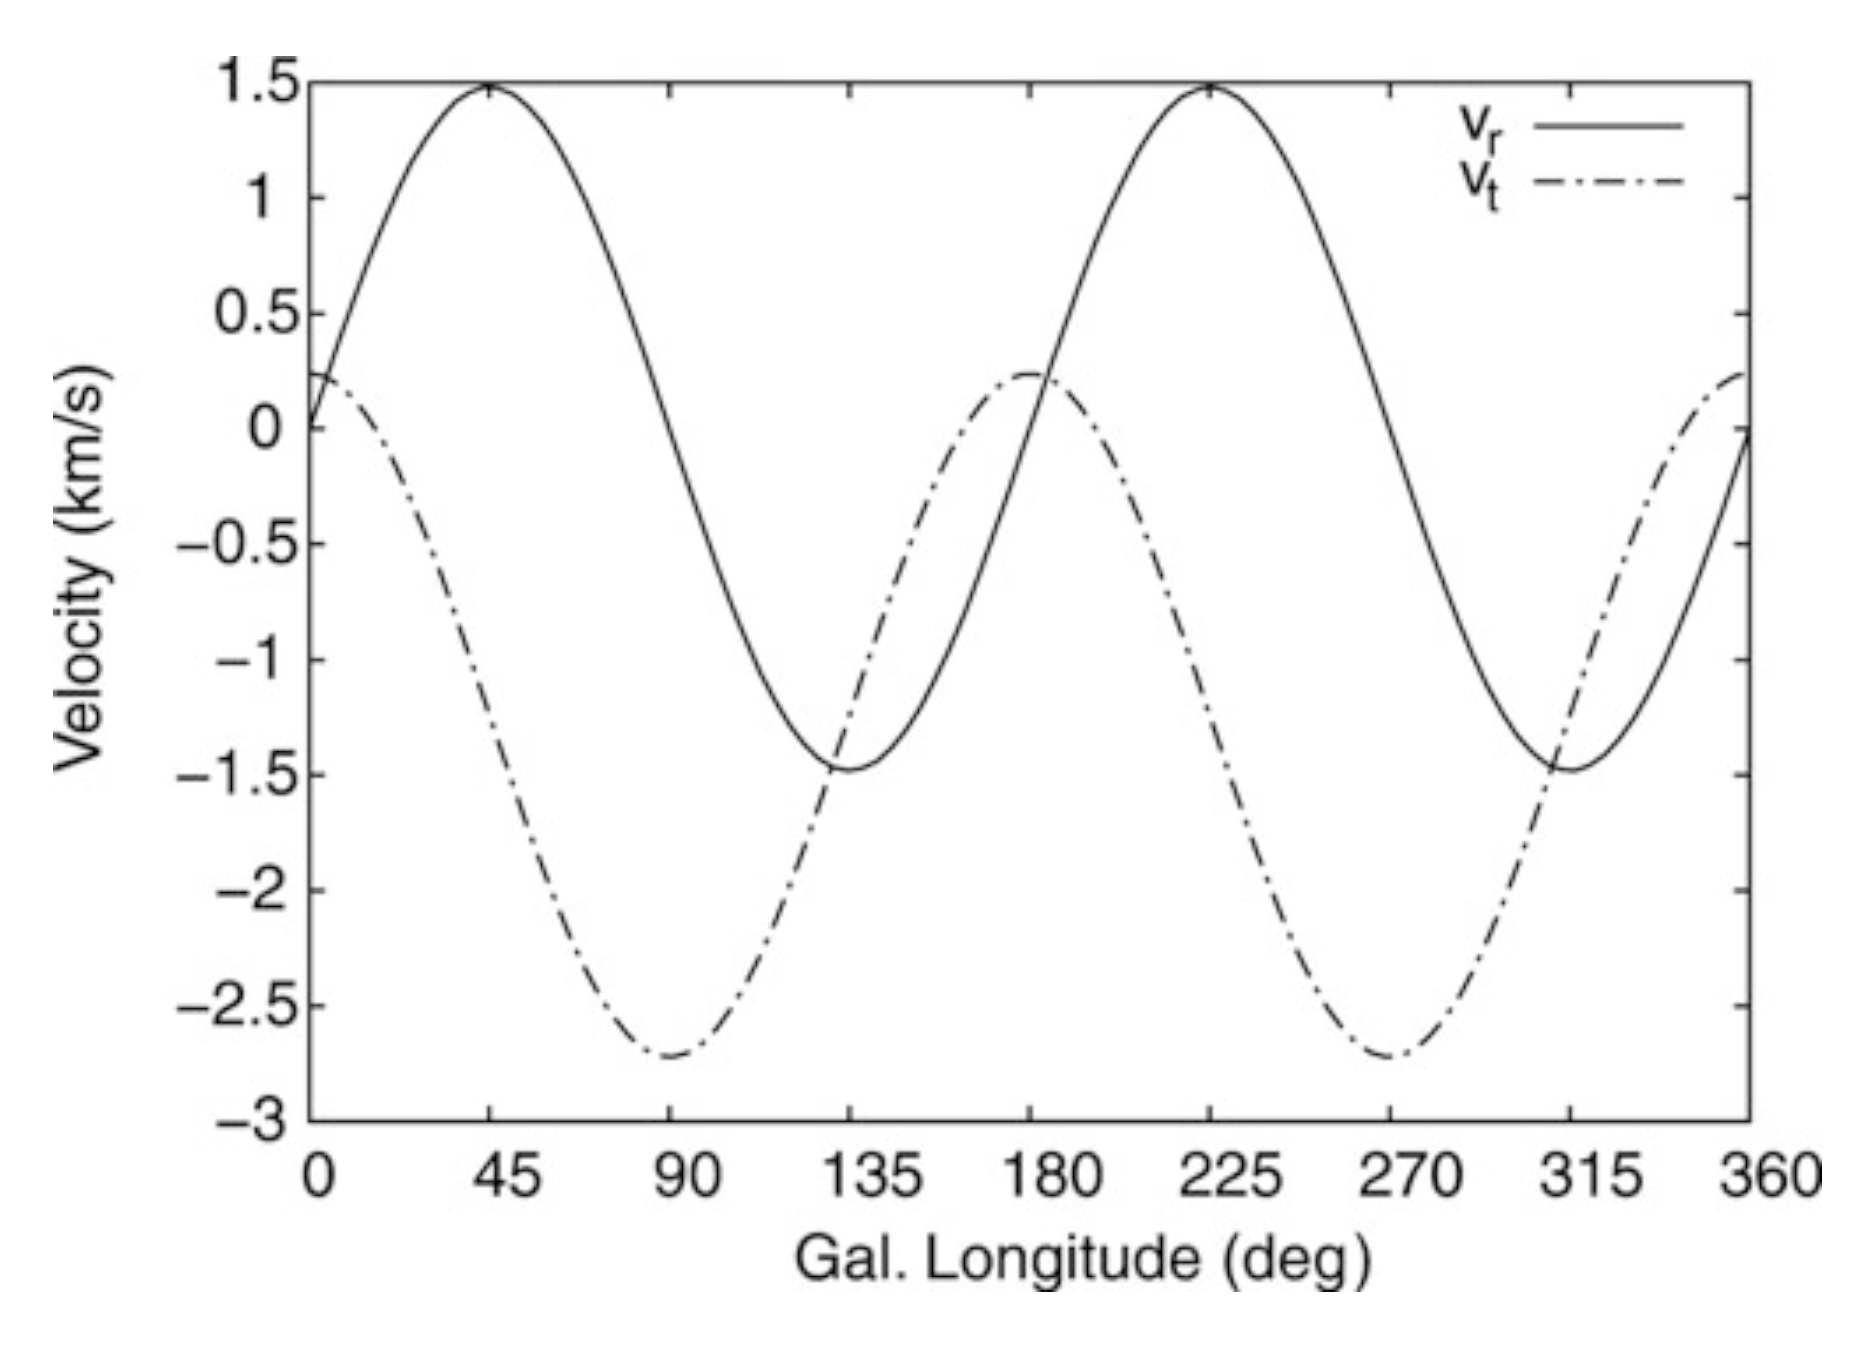
\includegraphics[width=10cm]{figures/vt_vr.png}}
\end{figure}

{\noindent}The radial and tangential velocity fields relative to the Sun show a sine curve with period $\pi$, where $_vt$ and $v_r$ are phase-shifted by $\pi/4$. This behavior of the velocity field in the Solar neighborhood is indeed observed (see Figure \ref{fig:vtvr}). By fitting the data for $v_r(\ell)$ and $v_t(\ell)$ for stars of equal distance $D$ one can determine $A$ and $B$, and thus

\begin{align*}
    \Omega_0 = \frac{V_0}{R_0} ~ [{\rm rad\,s^{-1}}] = A-B ~ [{\rm km\,s^{-1}\,kpc^{-1}}], ~~~ \left(\frac{{\rm d}V}{{\rm d}R}\right)_{R_0} = -(A+B) ~ [{\rm km\,s^{-1}\,kpc^{-1}}].
\end{align*}

{\noindent}The Oort constants thus yield the angular velocity of the Solar orbit and its derivative, and therefore the local kinematical information. If our Galaxy was rotating rigidly so that $\Omega$ was independent of the radius, $A=0$ would follow. But the Milky Way rotates differentially (i.e., the angular velocity depends on the radius). Measurements yield the following values for $A$ and $B$,

\begin{align*}
    A &= (14.8\pm0.8) ~ [{\rm km\,s^{-1}\,kpc^{-1}}] \\
    B &= (-12.4\pm0.6) ~ [{\rm km\,s^{-1}\,kpc^{-1}}].
\end{align*}

{\noindent}\textbf{Galactic rotation curve for $R<R_0$; tangent point method:} To measure the rotation curve for radii that are significantly smaller than $R_0$, one has to turn to large wavelengths due to extinction in the disk. Usually the $21\,{\rm cm}$ emission line of neutral hydrogen is used, which can be observed over large distances, or the emission of CO in molecular gas. These gas components are found throughout the disk and are strongly concentrated towards the plane. Furthermore, the radial velocity can easily be measured from the Doppler effect. However, since the distance to a hydrogen cloud cannot be determined directly, a method is needed to link the measured radial velocities to the distance of the gas from the Galactic center. For this purpose the tangent point method is used.

{\noindent}Consider a line-of-sight at fixed Galactic longitude $\ell$, with $\cos\ell>0$ (thus `inwards'). The radial velocity $v_r$ along this line-of-sight for objects moving on circular orbits is a function of the distance $D$, as found previously using the Oort constants. If $\Omega(R)$ is a monotonically decreasing function, $v_r$ attains a maximum where the line-of-sight is tangent to the local orbit, and thus its distance $R$ from the Galactic center attains the minimum value $R_{\rm min}$. This is the case at

\begin{align*}
    D = R_0\cos\ell ~ [{\rm kpc}], ~~~ R_{\rm min} = R_0\sin\ell ~ [{\rm kpc}]
\end{align*}

\begin{figure}[t]
    \centering
    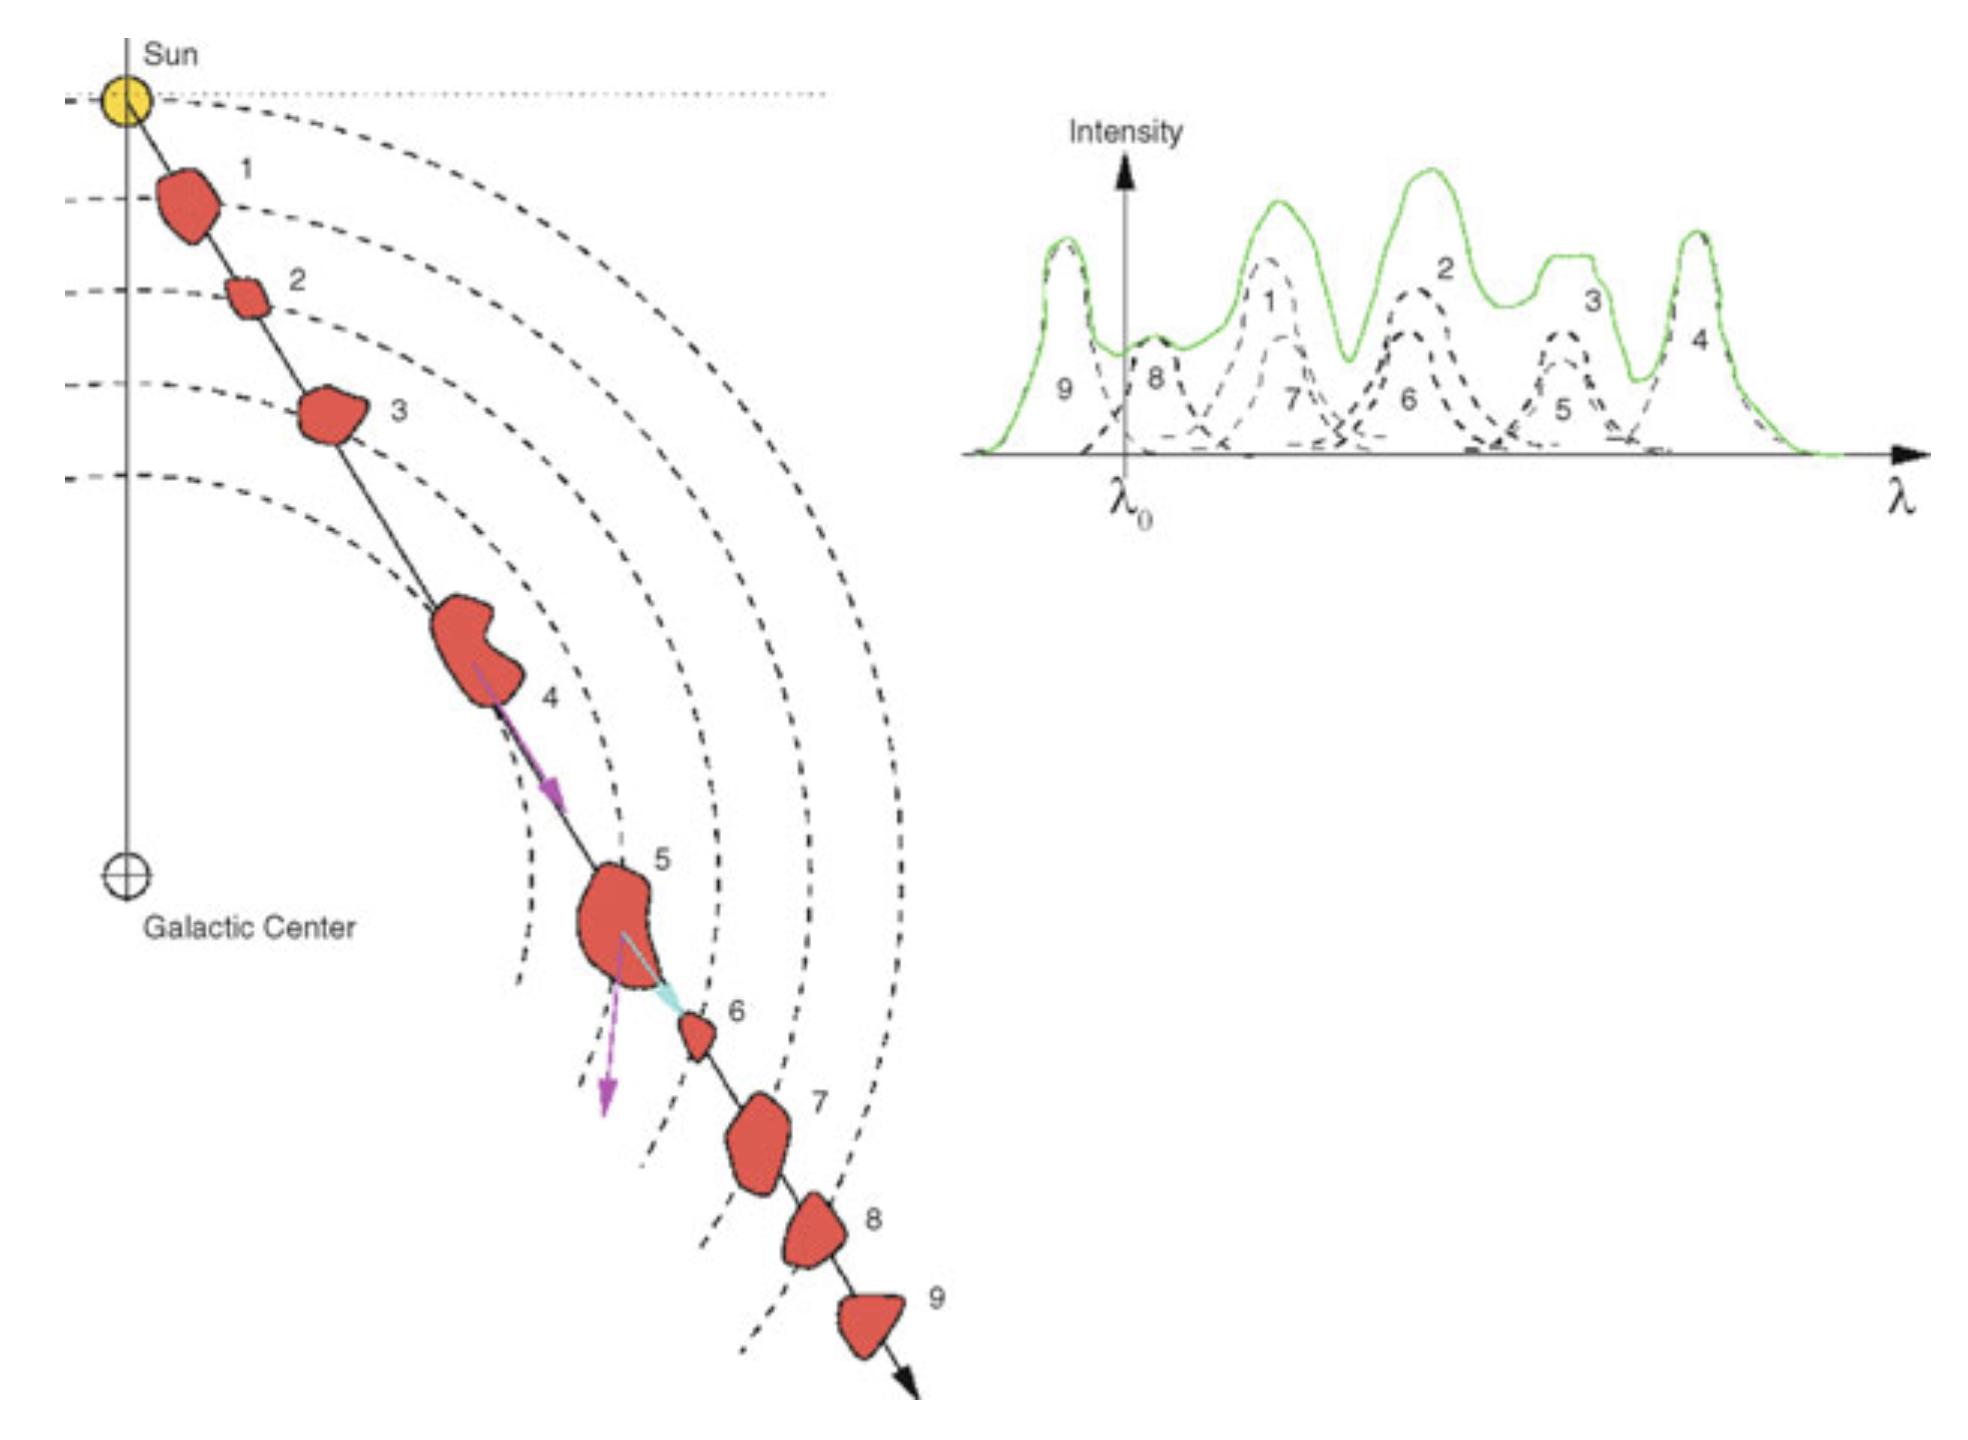
\includegraphics[width=12cm]{figures/TangentPoint.png}
    \caption{\footnotesize{The ISM is optically thin for $21\,{\rm cm}$ radiation, and thus we receive the $21\,{\rm cm}$ emission of HI regions from everywhere in the Galaxy. Due to the motion of an HI cloud relative to us, the wavelength is shifted. This can be used to measure the radial velocity of the cloud. With the assumption that the gas is moving on a circular orbit around the Galactic center, one expects that for the cloud in the tangent point (cloud 4), the full velocity is projected along the line-of-sight so that this cloud will therefore have the largest radial velocity. If the distance of the Sun to the Galactic center is known, the velocity of a cloud and its distance from the Galactic center can then be determined. Adopted from B.W. Carroll \& D.A. Ostlie 1996, Introduction to Modern Astrophysics, Addison-Wesley. Figure taken from Schneider (2015).}}
    \label{fig:tangentpoint}
\end{figure}

{\noindent}(see Figure \ref{fig:tangentpoint}). The maximum radial velocity there, to equations derived above with the Oort constants, is

\begin{align*}
v_{r,\mathrm{max}} = [\Omega(R_{\rm min}-\Omega_0)] R_0\sin\ell = V(R_{\rm min}) - V_0\sin\ell ~[{\rm km\,s^{-1}}],
\end{align*}

{\noindent}so that from the measured value of $v_{r,{\rm max}}$ as a function of direction $\ell$, the rotation curve inside $R_0$ can be determined,

\begin{align*}
    V(R) = \left(\frac{R}{R_0}\right)V_0 + v_{r,{\rm max}}(\sin\ell=R/R_0) ~ [{\rm km\,s^{-1}}].
\end{align*}

{\noindent}In the optical regime of the spectrum this method can only be applied locally, i.e., for small $D$, due to extinction. This is the case if one observes in a direction nearly tangential to the orbit of the Sun, i.e., if $0<\pi/2-\ell\ll1$ or $0<\ell-3\pi/2\ll1$, or $\lvert\sin\ell\rvert\approx1$, so that $R_0-R_{\rm min}\ll R_0$. In this case we get, to first order in $(R_0-R_{\rm min})$,

\begin{align}
    V(R_{\rm min}) &\approx V_0 \left(\frac{{\rm d}V}{{\rm d}R}\right)_{R_0}(R_{\rm min}-R_0) \\
    &= V_0 - \left(\frac{{\rm d}V}{{\rm d}R}\right)_{R_0} R_0(1-\sin\ell) ~ [{\rm km\,s^{-1}}],
\end{align}

{\noindent}Applying this to our equation for $v_{r,{\rm max}}$,

\begin{align*}
    v_{r,{\rm max}} &= \left[V_0-\left(\frac{{\rm d}V}{{\rm d}R}\right)_{R_0}R_0\right](1-\sin\ell) \\
    &= 2AR_0(1-\sin\ell) ~ [{\rm km\,s^{-1}}],
\end{align*}

{\noindent}This relation can also be used for determining the Oort constant A.

{\noindent}To determine $V(R)$ for smaller $R$ by employing the tangent point method, we have to observe in wavelength regimes in which the Galactic plane is transparent, using radio emission lines of gas. In Figure \ref{fig:vLSRvslong}, a typical intensity profile of the $21\,{\rm cm}$ line along a line-of-sight is sketched; according to the Doppler effect this can be converted directly into a velocity profile using $v_r=(\lambda-\lambda_0)\lambda_0$. It consists of several maxima that originate in individual gas clouds. The radial velocity of each cloud is defined by its distance $R$ from the Galactic center (if the gas follows the Galactic rotation), so that the largest radial velocity will occur for gas closest to the tangent point, which will be identified with $v_{r,{\rm max}}(\ell)$. Figure 2.28 shows the observed intensity profile of the $^{12}$CO line as a function of the Galactic longitude, from which the rotation curve for $R<R_0$ can be read off.

\begin{figure}[h]
    \floatbox[{\capbeside\thisfloatsetup{capbesideposition={right,top},capbesidewidth=4cm}}]{figure}[\FBwidth]
    {\caption{\footnotesize{$^{12}$CO emission of molecular gas in the Galactic disk. For each $\ell$, the intensity of the emission in the $\ell-v_r$ plane is plotted, integrated over the range $-2^\circ\leq b \leq2^\circ$ (i.e., very close to the middle of the Galactic plane). Since $v_r$ depends on the distance along each line- of-sight, characterized by $\ell$, this diagram contains information on the rotation curve of the Galaxy as well as on the spatial distribution of the gas. The maximum velocity at each $\ell$ is rather well defined and forms the basis for the tangent point method. Source: P. Englmaier \& O. Gerhard 1999, Gas dynamics and large-scale morphology of the Milky Way galaxy, MNRAS 304, 512, p. 514, Fig. 1. Figure taken from Schneider (2015).}}
    \label{fig:vLSRvslong}}
    {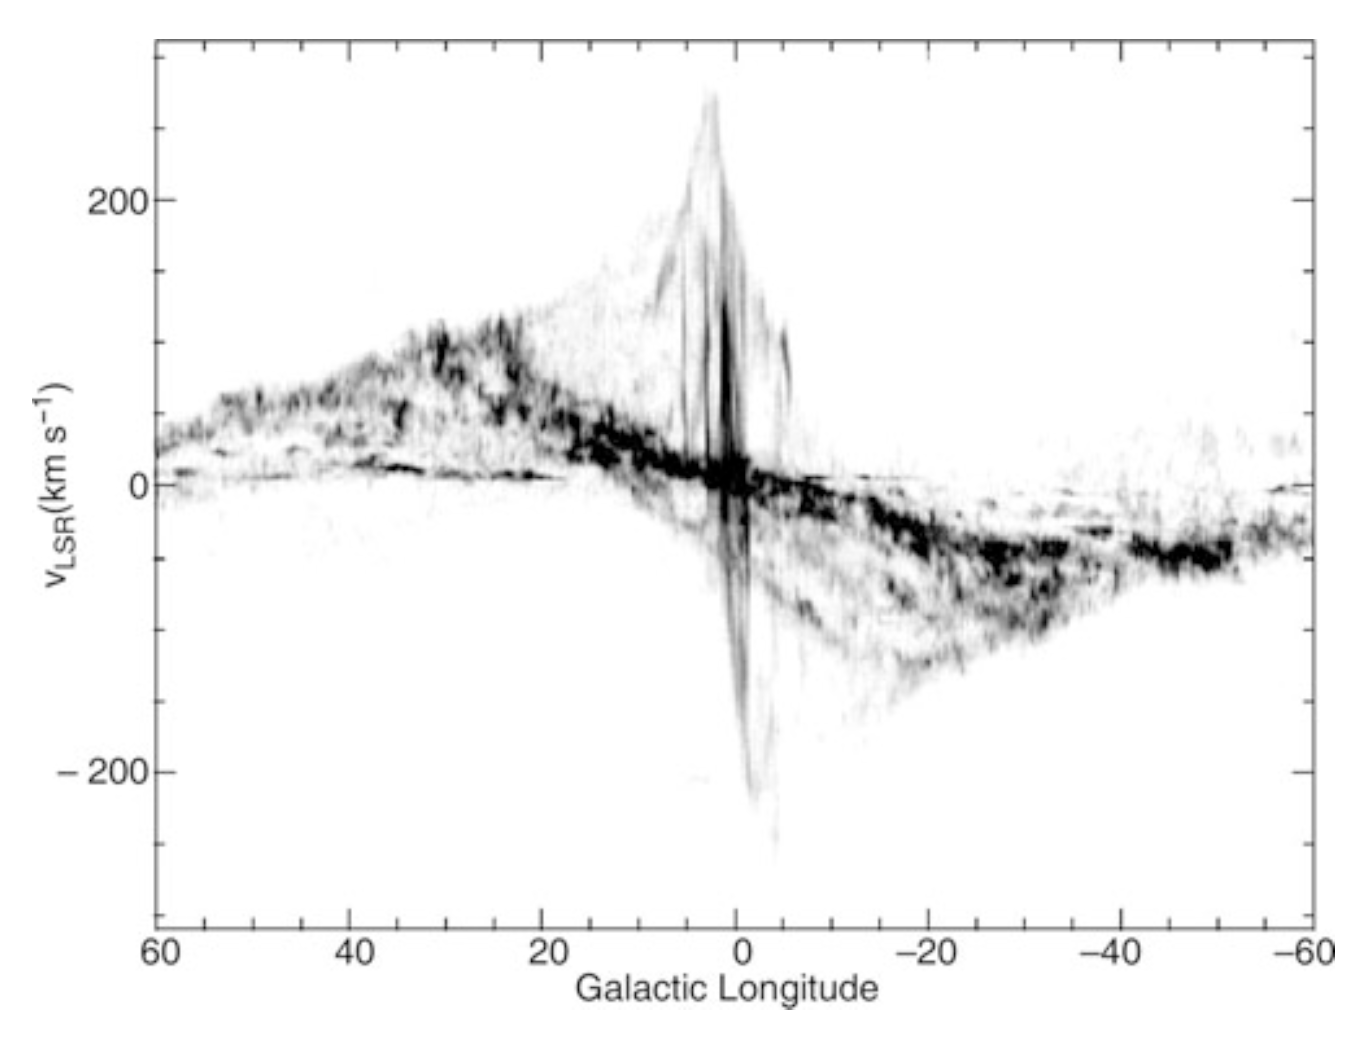
\includegraphics[width=10cm]{figures/vLSRvslong.png}}
\end{figure}

{\noindent}\textit{With the tangent point method, applied to the $21\,{\rm cm}$ line of neutral hydrogen or to radio emission lines of molecular gas, the rotation curve of the Galaxy inside the Solar orbit (i.e., for $R<R_0$) can be measured.}

{\noindent}\textbf{Rotation curve for $R>R_0$:} The tangent point method cannot be applied for $R>R_0$ because for lines-of-sight at $\pi/2<\ell<3\pi/2$, the radial velocity $v_r$ attains no maximum. In this case, the line-of-sight is nowhere parallel to a circular orbit. 

{\noindent}Measuring $V(R)$ for $R>R_0$ requires measuring $v_r$ for objects whose distance can be determined directly (e.g., Cepheids, for which the period-luminosity relation is used, or O- and B-stars in HII-regions). With $\ell$ and $D$ known, $R$ can then be calculated which allows us to obtain $\Omega(R)$ or $V(R)$, respectively. Any object with known $D$ and $v_r$ thus contributes one data point to the Galactic rotation curve. Since the distance estimates of individual objects are always affected by uncertainties, the rotation curve for large values of $R$ is less accurately known than that inside the Solar circle. Recent measurements of blue horizontal-branch stars within the outer halo of the MW by SDSS yielded an estimate of the rotation curve out to $r\sim60\,{\rm kpc}$. The situation will improve dramatically once the results from Gaia will become available: Gaia will measure distances via trigonometric parallaxes, and proper motions of many star outside the Solar circle.

{\noindent}It turns out that the rotation curve for $R>R_0$ does not decline outwards (see Figure \ref{fig:rotationcurve}) as we would expect from the distribution of visible matter in the MW. Both the stellar density and the gas density of the Galaxy decline exponentially for large $R$. This steep radial decline of the visible matter density should imply that $M(R)$, the mass inside $R$, is nearly constant for $R\gtrsim R_0$, from which a velocity profile like $V\propto R^{-1/2}$ would follow, according to Kepler's law. However, this is not the case: $V(R)$ is virtually constant for $R>R_0$, indicating that $M(R)\propto R$. In fact, a small decrease to about $180,{\rm km\,s^{-1}}$ at $R=60\,{\rm kpc}$ was estimated, corresponding to a total mass of $(4.0\pm0.7)\times10^{11}\,{\rm M_\odot}$ enclosed within the inner $60\,{\rm kpc}$, but this decrease is much smaller than expected from Keplerian rotation. In order to get an almost constant rotational velocity of the Galaxy, much more matter has to be present than we observe in gas and stars.

{\noindent}\textit{The MW contains, besides stars and gas, an additional component of matter that dominates the mass at $R\gtrsim R_0$. Its presence is known only by its gravitational effect, since it has not been observed directly yet, neither in emission nor in absorption. Hence, it is called \textbf{dark matter}.} This is a common phenomenon: the rotation curves of spiral galaxies are flat up to the maximum radius at which they can be measured; spiral galaxies contain dark matter. A better way of phrasing is would be to say that the visible galaxy is embedded in a dark matter halo, since the total mass of the MW (and other spiral galaxies) is dominated by dark matter.

{\noindent}\textbf{Rotation curves and dark matter:} The rotation curves of other spiral galaxies are easier to measure than that of the MW because we are able to observe them `from outside'. These measurements are achieved by utilizing the Doppler effect, where the inclination of the disk (i.e., its orientation with respect to the line-of-sight) has to be accounted for. The inclination angle is determined from the observed axis ratio of the disk, assuming that disks are intrinsically axially symmetric (except for the spiral arms). Mainly the stars and HI gas in the galaxies are used as luminous tracers, where the observable HI disk is in general significantly more extended than the stellar disk. Therefore, the rotation curves measured from the $21\,{\rm cm}$ line typically extend to much larger radii than those from optical stellar spectroscopy.

{\noindent}Like our MW, other spirals also rotate considerably faster in their outer regions than one would expect from Kepler's law and the distribution of visible matter (see Figure \ref{fig:rotationcurvesspirals}).

\begin{figure}[h]
    \floatbox[{\capbeside\thisfloatsetup{capbesideposition={right,top},capbesidewidth=4cm}}]{figure}[\FBwidth]
    {\caption{\footnotesize{Examples of rotation curves of spiral galaxies. They are all flat in the outer region and do not behave as expected from Kepler's law if the galaxy consisted only of luminous matter. Also striking is the fact that the amplitude of the rotation curve is higher for early-type than for late-type spirals. Source: V. Rubin et al. 1978, Extended rotation curves of high-luminosity spiral galaxies. IV—Systematic dynamical properties, SA through SC, ApJ 225, L107, p. L109, Fig. 3. Figure taken from Schneider (2015).}}
    \label{fig:rotationcurvesspirals}}
    {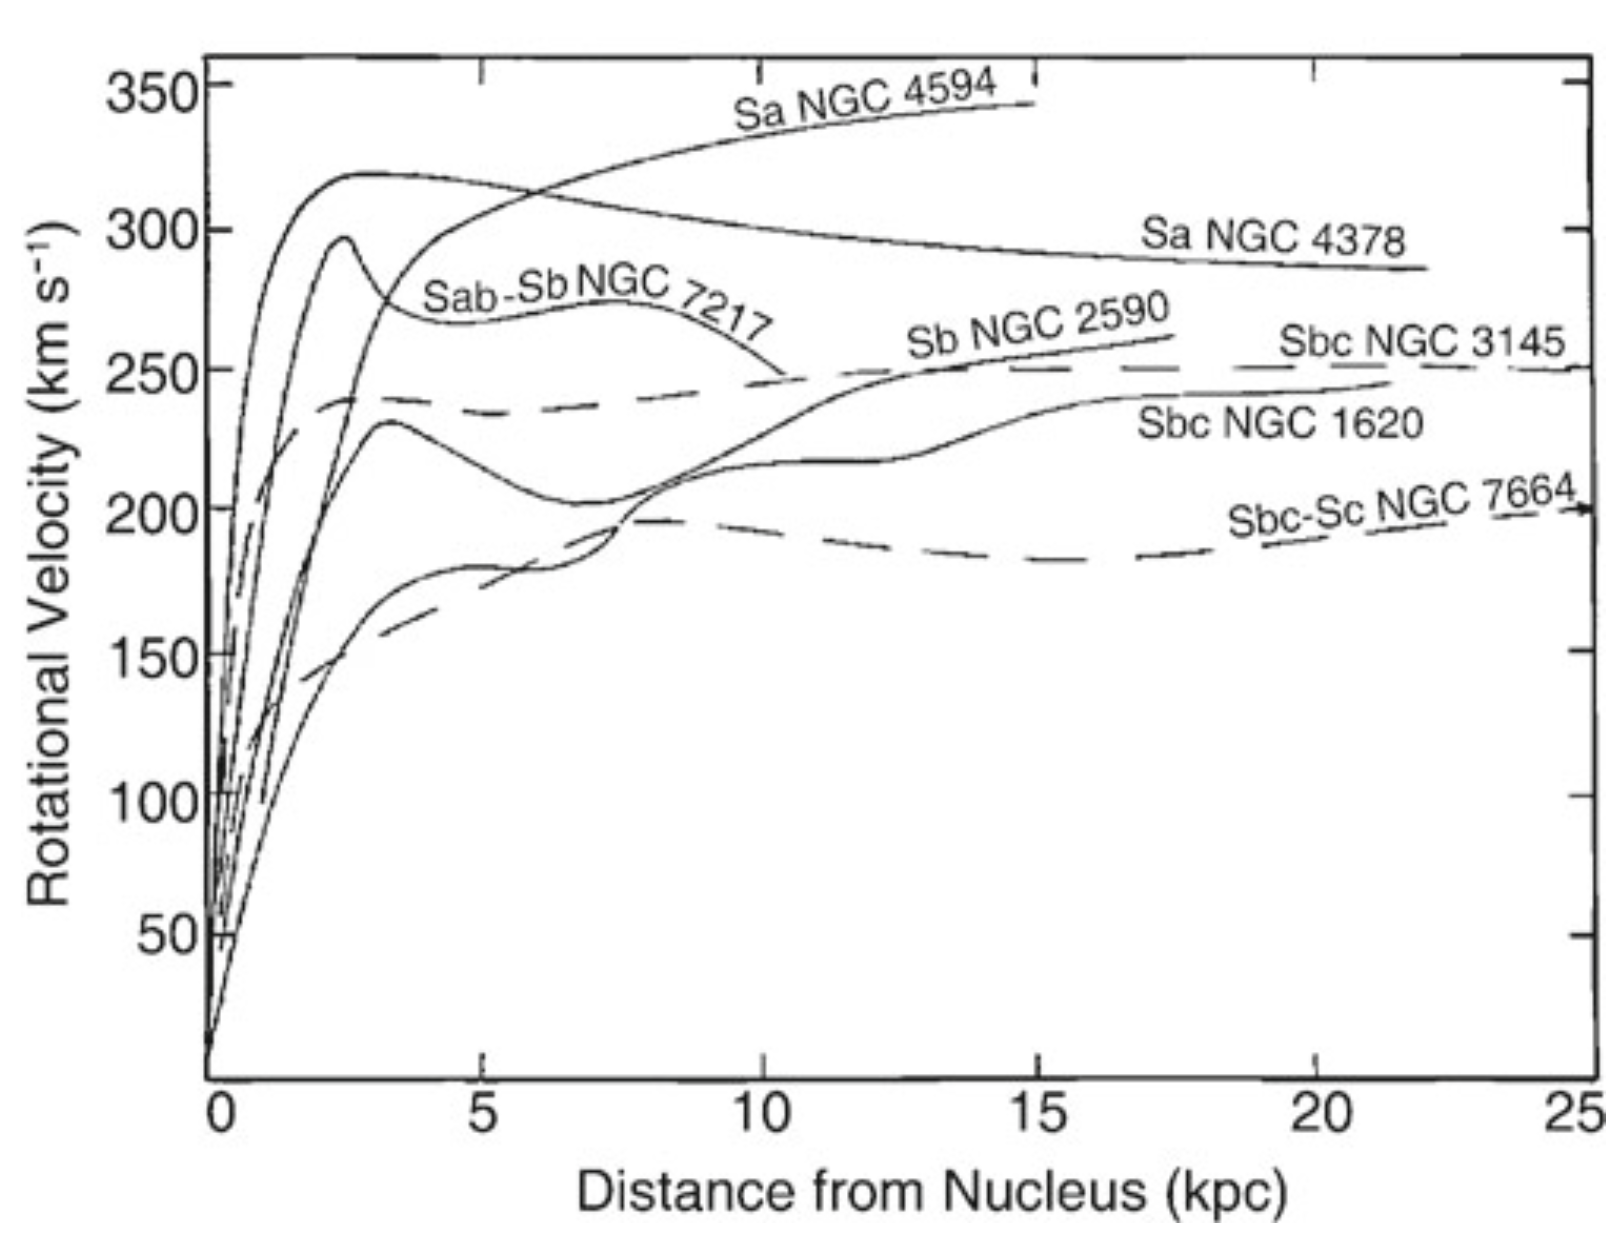
\includegraphics[width=10cm]{figures/RotationCurves_spirals.png}}
\end{figure}

{\noindent}\textit{The rotation curves of spirals do not decrease for $R\geq h_R$, as one would expect from the light distribution, but are basically flat. We therefore conclude that spirals are surrounded by a halo of dark matter. The density distribution of this dark halo can be derived from the rotation curves.}

{\noindent}To see how the density distribution of the dark matter can be derived from the rotation curves, we employ the force balance between gravitation and centrifugal acceleration, as described by the Kepler rotation law,

\begin{align*}
    v^2(R) = \frac{GM(R)}{R} ~ [{\rm km^2\,s^{-2}}],
\end{align*}

{\noindent}from which one directly obtains the mass $M(R)$ within a radius $R$. The rotation curve expected from the visible matter distribution is\footnote{This consideration is strongly simplified insofar as the given relations are only valid in this form for spherical mass distributions. The rotational velocity produced by an oblate (disk-shaped) mass distribution is more complicated to calculate; for instance, for an exponential mass distribution in a disk, the maximum of $v_{\rm lum}$ occurs at   $\sim2.2h_R$, with a Kepler decrease, $v_{\rm lum}\propto R^{-1/2}$, at larger radii.}

\begin{align*}
    v_{\rm lum}^2 = \frac{GM_{\rm lum}(R)}{R} ~ [{\rm km^2\,s^{-2}}].
\end{align*}

{\noindent}$M_{\rm lum}(R)$ can be determined by assuming a plausible value for the mass-to-light ratio $M/L4$ of the luminous matter. This value is obtained either from the spectral light distribution of the stars, together with knowledge of the properties of stellar populations, or by fitting the innermost part of the rotation curve (where the mass contribution of dark matter can presumably be neglected), assuming that $M/L$ is independent of radius for the stellar population. From this estimate of the mass-to-light ratio, the discrepancy between $v_{\rm lum}^2$ and $v^2$ yields the distribution of the dark matter, $v_{\rm dark}^2=v^2-v_{\rm lum}^2=GM_{\rm dark}/R$, or

\begin{align*}
    M_{\rm dark}(R) = \frac{R}{G} [v^2(R) - v_{\rm lum}^2(R)] ~ [{\rm M_\odot}].
\end{align*}

{\noindent}An example of this decomposition of the mass contributions is shown in Figure \ref{fig:rotationcurvedecomp}.

\begin{figure}[h]
    \floatbox[{\capbeside\thisfloatsetup{capbesideposition={right,top},capbesidewidth=4cm}}]{figure}[\FBwidth]
    {\caption{\footnotesize{The flat rotation curves of spiral galaxies cannot be explained by visible matter alone. The example of NGC 3198 demonstrates the rotation curve which would be expected from the visible matter alone (curve labeled `disk'). To explain the observed rotation curve, a dark matter component has to be present (curve labeled `halo'). However, the decomposition into disk and halo mass is not unambiguous because for it to be so it would be necessary to know the mass-to-light ratio of the disk. In the case considered here, a `maximum disk' was assumed (i.e., it was assumed that the innermost part of the rotation curve is produced solely by the visible matter in the disk). Source: T.S. van Albada et al. 1985, Distribution of dark matter in the spiral galaxy NGC 3198, ApJ 295, 305, p. 309, Fig. 4. Figure taken from Schneider (2015).}}
    \label{fig:rotationcurvedecomp}}
    {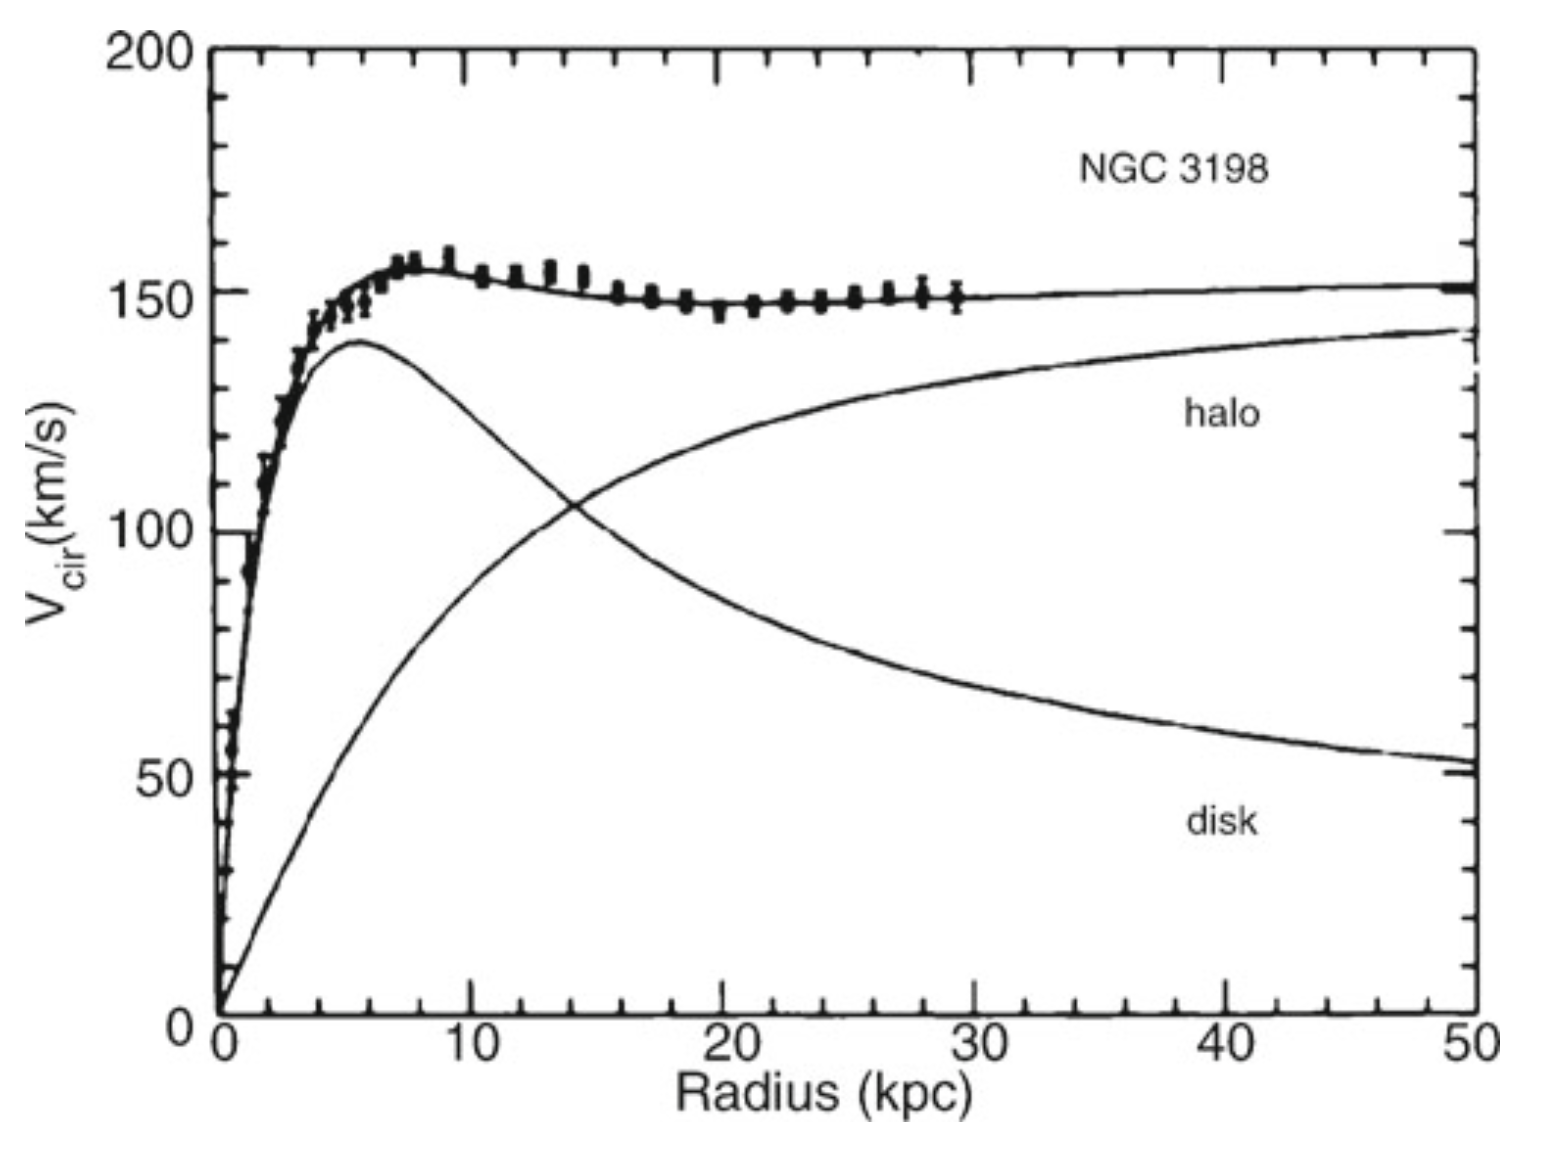
\includegraphics[width=12cm]{figures/RotationCurve_decomp.png}}
\end{figure}

{\noindent}The corresponding density profiles of the dark matter halos seem to be flat in the inner region, and decreasing as $R^{-2}$ at large radii. It is remarkable that $\rho\propto R^{-2}$ implies a mass profile $M\propto R$ (i.e., the mass of the halo increases linearly with the radius for large R). As long as the extent of the halo is undetermined the total mass of a galaxy will be unknown. Since the observed rotation curves are flat out to the largest radius for which $21\,{\rm cm}$ emission can still be observed, a lower limit for the radius of the dark halo can be obtained, $R_{\rm halo}\gtrsim30h^{-1}\,{\rm kpc}$. Inside the optical radius of a disk, the dark matter comprises about $2/3$ of the total mass.

{\noindent}To derive the density profile out to even larger radii, other observable objects in an orbit around the galaxies are needed. Potential candidates for such luminous tracers are satellite galaxies -- companions of other spirals, like the Magellanic Clouds are for the MW. Because we cannot presume that these satellite galaxies move on circular orbits around their parent galaxy, conclusions can be drawn based only on a statistical sample of satellites. These analyses of the relative velocities of satellite galaxies around spirals still give no indication of an `edge' to the halo, leading to a lower limit for the radius of $R_{\rm halo}\gtrsim100h^{-1}\,{\rm kpc}$.

\subsubsection{Follow-up Questions}

\begin{itemize}
    \item What assumptions are made in deriving the $1/r^2$ profile?
\end{itemize}

% --------------------------------------------------------------
%               15. 
% --------------------------------------------------------------

\newpage
\subsection{Question 15}

What thermal phases are postulated to exist in the interstellar medium? Describe the dominant mechanism of cooling for each phase.

\subsubsection{Short answer}

Answer.

\subsubsection{Additional context}

Interstellar matter accounts for $\sim10-15\%$ of the total
mass of the Galactic disk. It tends to concentrate near the Galactic plane and along the spiral arms, while being very inhomogeneously distributed at small scales. Roughly half the interstellar mass is confined to discrete clouds occupying only $\sim1-2\%$ of the interstellar volume. These interstellar clouds can be divided into three types: the \textbf{dark clouds}, which are essentially made of very cold ($T\sim10-20\,{\rm K}$) molecular gas and block off the light from background stars, the \textbf{diffuse clouds}, which consist of cold ($T\sim100\,{\rm K}$) atomic gas and are almost transparent to the background starlight, except at a number of specific wavelengths where they give rise to absorption lines, and the \textbf{translucent clouds}, which contain molecular and atomic gases and have intermediate visual extinctions. The rest of the interstellar matter, spread out between the clouds, exists in three different forms: \textbf{warm (mostly neutral) atomic}, \textbf{warm ionized}, and \textbf{hot ionized}, where warm refers to a temperature of $10^4\,{\rm K}$ and hot to a temperature of $10^6\,{\rm K}$ (see Table \ref{table:ISMphases}).

\begin{table}[h]
    \centering
    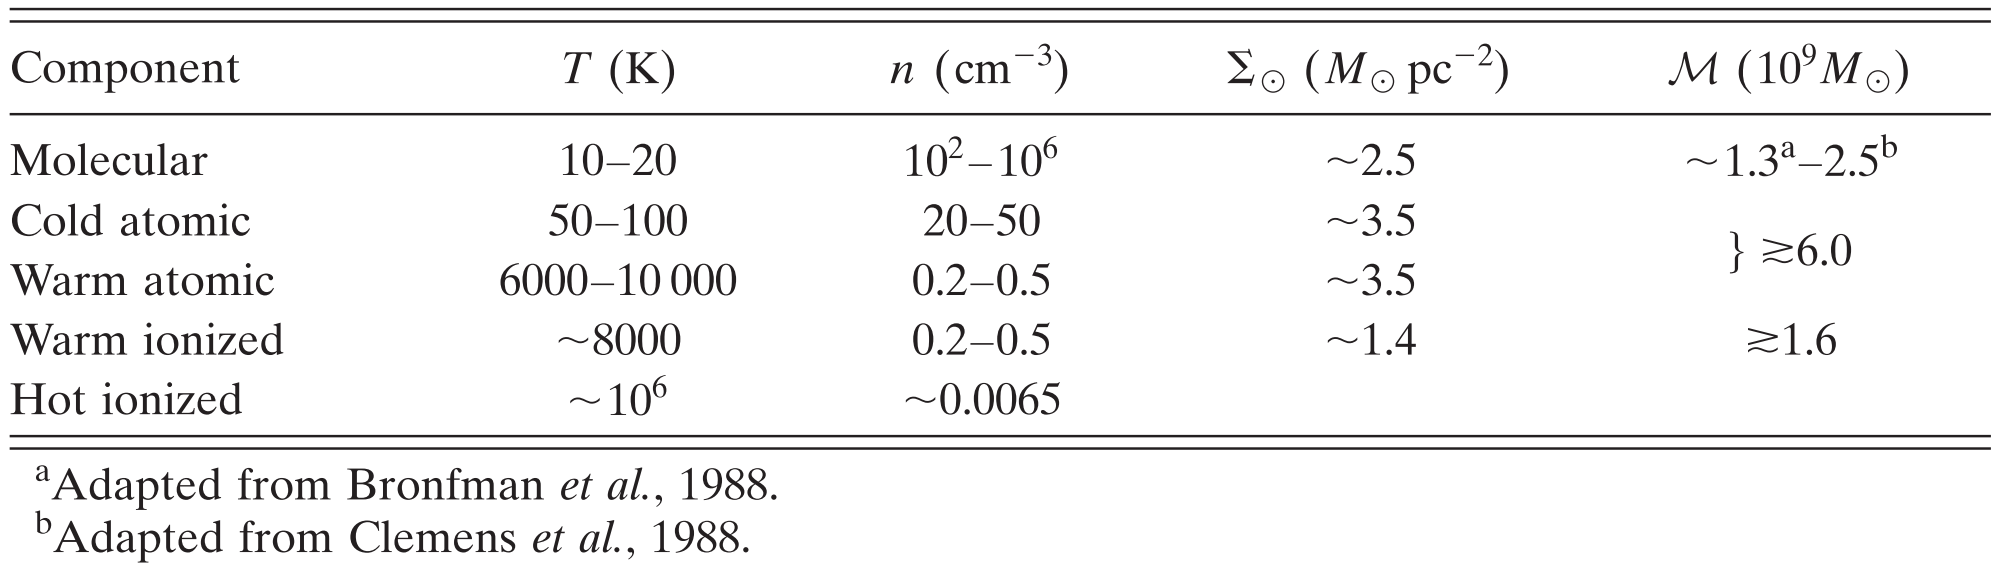
\includegraphics[width=14cm]{figures/ISMphases_table.png}
    \caption{\footnotesize{Descriptive parameters of the different components of the interstellar gas. $T$ is the temperature, $n$ is the true (as opposed to space-averaged) number density of hydrogen nuclei near the Sun, $\Sigma_\odot$ is the azimuthally averaged mass density per unit area at the solar circle, and $\mathcal{M}$ is the mass contained in the entire Milky Way. Both $\Sigma_\odot$ and $\mathcal{M}$ include 70.4\% hydrogen, 28.1\% helium, and 1.5\% heavier elements. All values were rescaled to $R_\odot=8.5\,{\rm kpc}$. Figure taken from Ferri\`ere (2001).}}
    \label{table:ISMphases}
\end{table}

{\noindent}\textbf{Molecular gas:} The H$_2$ molecule itself is not directly observable at radio wavelengths: because it possesses no permanent electric dipole moment and has a very small moment of inertia, all its permitted transitions lie outside the radio domain. The CO molecule, for its part, has a $J=1\rightarrow0$ rotational transition at a radio wavelength of $2.6\,{\rm mm}$; the corresponding emission line, which was first observed a few months before the detection of CO in UV absorption, has become the primary tracer of molecular interstellar gas.

{\noindent}\textbf{Neutral atomic gas:} Neutral atomic hydrogen, usually denoted by HI (as opposed to HII for ionized hydrogen), is not directly observable at optical wavelengths. Under most interstellar conditions, particle collisions are so infrequent that nearly all hydrogen atoms have their electron in the ground energy level $n=1$. It turns out that all the electronic transitions between the ground level and an excited state (forming the Lyman series) lie in the UV, with the Lyman $\alpha$ (Ly$\alpha$) transition between the ground level and the first excited state $n=2$ occurring at a wavelength of $1216$\AA.

{\noindent}The breakthrough event that opened the era of radio-astronomical observations of interstellar HI was the detection of the interstellar $21\,{\rm cm}$ line emission. The existence of the $21\,{\rm cm}$ line results from the ``hyperfine'' structure of the hydrogen atom. In brief, the interaction between the magnetic moment of the electron and that of the proton leads to a splitting of the electronic ground level into two extremely close energy levels, in which the electron spin is either parallel (upper level) or anti-parallel (lower level) to the proton spin. It is the ``spin-flip'' transition between these two energy levels that corresponds to the now famous $21\,{\rm cm}$ line. The major advantage of $21\,{\rm cm}$ photons resides in their ability to penetrate deep into the ISM, thereby offering a unique opportunity to probe the interstellar HI gas out to the edges of the MW. On the other hand, the highly forbidden spin-flip transition is intrinsically so rare (Einstein A coefficient $A_{21}=2.85\times10^{-15}\,{\rm s^{-1}}$) that very long paths are needed for the $21\,{\rm cm}$ line to be detectable.

\begin{figure}[t]
    \floatbox[{\capbeside\thisfloatsetup{capbesideposition={right,top},capbesidewidth=4cm}}]{figure}[\FBwidth]
    {\caption{\footnotesize{$21\,{\rm cm}$ spectra of HI gas. The $x$ axis is gas velocity along the line of sight (in ${\rm km\,s^{-1}}$) and the $y$ axis is intensity in arbitrary units. \textbf{(Top:)} Emission line profile nearby to the direction toward an HII region. \textbf{(Bottom:)} The absorption spectrum, which can represent only relatively cool gas exactly along the line of sight to the HII region. Figure taken from Ferri\`ere (2001).}}
    \label{fig:21cmemissabs}}
    {\includegraphics[width=10cm]{figures/21cm_emission_abs.png}}
\end{figure}

{\noindent}The $21\,{\rm cm}$ absorption spectra generally look quite different from emission spectra taken in a nearby direction: while the emission spectra contain both distinct narrow peaks and much broader features, only the narrow peaks are present in the absorption spectra (see Figure \ref{fig:21cmemissabs}). The conventional interpretation of this difference is that the narrow peaks seen in emission and in absorption are produced by discrete cold ($T\sim5-100\,{\rm K}$) H I clouds, whereas the broader features seen in emission only are due to a widespread HI gas that is too warm to give rise to detectable $21\,{\rm cm}$ absorption. The estimated temperature of the warm HI component is $T\sim6000-10000\,{\rm K}$.

{\noindent}\textbf{Warm ionized gas:} O and B stars, the hottest and most massive stars in the MW, emit a strong UV radiation, which, below a wavelength of $912$\AA~(corresponding to an energy of $13.6\,{\rm eV}$), is sufficiently energetic to ionize hydrogen atoms. As a result, these stars are surrounded by a so-called ``\textbf{HII region}'' within which hydrogen is almost fully ionized. Given that the ionizing UV photons are promptly absorbed by neutral hydrogen, the transition between the HII region and the ambient ISM is rather abrupt. Inside the HII region, ions and free electrons keep recombining before being separated again by fresh UV photons from the central star. Thus the HII region grows until the rate of recombinations within it becomes large enough to balance the rate of photoionizations. In a uniform medium, this balance occurs when the radius of the HII region reaches the value of the \textbf{Str\"omgren radius},

\begin{align*}
    r_s = 30 \left(\frac{N_{48}}{n_{\rm H}n_e}\right)^{1/3} ~ [{\rm pc}],
\end{align*}

{\noindent}where $N_{48}$ is the number of ionizing photons emitted per unit time by the central star, in $10^{48}\,{\rm s^{-11}}$ (e.g., $N_{48}\approx34$ for an O5V star and $N_{48}\approx1.7$ for a B0V star), and $n_{\rm H}$ and $n_e$ are the free-proton and free-electron number densities in the HII region, in ${\rm cm^{-3}}$.

{\noindent}The process of photoionization is accompanied by a
net heating of the interstellar gas, as the ionizing photons transfer a fraction of their energy (the excess with respect to the ionization potential) to the ejected electrons. The equilibrium temperature, set by a balance between photoelectric heating and radiative cooling, has a typical value $\sim8000\,{\rm K}$, depending on density and metallicity. This theoretical estimate turns out to be in good agreement with observational determinations based on measurements of the radio continuum radiation and on studies of emission-line ratios from HII regions.

{\noindent}The radio continuum radiation of an HII region arises
from the \textbf{bremsstrahlung or} ``\textbf{free-free}'' emission generated as free electrons are accelerated in the Coulomb field of positive ions (H$^+$,He$^+$,He$^{2+}$). Emission lines, found at optical, IR, and radio wavelengths, are primarily due to radiative recombination of hydrogen and helium ions with free electrons and to radiative de-excitation of collisionally excited ionized metals. Of special importance are the optical hydrogen \textbf{Balmer lines} produced by electronic transitions from an excited state $n>2$ to the first excited state $n=2$. Because each recombination of a free proton with a free electron into an excited hydrogen atom leads sooner or later to the emission of one Balmer photon, and because the rate per unit volume of recombinations into an excited hydrogen atom is proportional to $N_{\rm H^+} + n_e \propto n_e^2$, the integrated intensity of the Balmer lines is directly proportional to the \textbf{emission measure}

\begin{align*}
    {\rm EM} = -\int\limits_{\rm source}^{\rm observer}n_e^2{\rm d}s ~ [{\rm pc\,cm^{-6}}],
\end{align*}

{\noindent}where ${\rm d}s$ is the length element along the line of sight through the HII region. For future reference, let us specify that the hydrogen Balmer transition between the electronic energy levels $n=3$ and $n=2$ is usually referred to as the $\mathbf{H\alpha}$ transition and has a wavelength of $6563$\,\AA.

{\noindent}\textbf{Hot ionized gas:} The notion that hot interstellar gas exists in the MW dates back to Spitzer's (1956) paper on a possible Galactic corona, made of hot rarefied gas, which would provide the necessary pressure to confine the observed high-altitude interstellar clouds. The presence of such a hot gas was borne out almost two decades later by two independent types of observations: (1) the Copernicus satellite detected, in the spectrum of several bright stars, broad UV absorption lines of high-stage ions that form only at elevated temperatures, and (2) the observed soft-x-ray background radiation was found to be most likely due to thermal emission from a hot interstellar plasma.

{\noindent}Amongst the high-stage ions accessible to UV observations, OVI (five-times-ionized oxygen, with a doublet at ($1032$\AA, $1038$\AA)) and NV (four-times-ionized nitrogen, with a doublet at ($1239$\AA, $1243$\AA)) are the best tracers of hot collisionally ionized gas, insofar as their high ionization potential makes them difficult to produce by photoionization.

{\noindent}The soft-x-ray background radiation around $0.25\,{\rm keV}$ appears to arise predominantly from the Local Bubble. It is very likely that $0.25\,{\rm keV}$ x-ray-emitting regions exist throughout the MW, but because their radiation is efficiently absorbed by the intervening cool interstellar gas, the majority of them must escape detection. On the other hand, a number of bright features have been observed in the intermediate energy band $0.5-1.0\,{\rm keV}$, which is less affected by photoelectric absorption. Most of these features were shown to be associated either with individual supernova remnants (produced by isolated supernova explosions) or with ``\textbf{superbubbles}'' (produced by the joint action of stellar winds and supernova explosions in a group of massive stars), and their x-ray radiation was attributed to thermal emission from a hot plasma at a temperature of a few $10^6\,{\rm K}$.

{\noindent}It is now widely accepted that the hot interstellar gas is generated by SN explosions and, to a lesser extent, by the generally powerful winds from the progenitor stars.

{\noindent}Figures \ref{fig:ISMdisk}, \ref{fig:ISMvertical}, and \ref{fig:ISMglobal} show the various components of the ISM within the Galactic disk, about $300\,{\rm pc}$ of the midplane, and larger scale structure of the Galactic atmosphere, respectively. In these figures, purple indicates dark molecular clouds; solid green-cold HI clouds; hatched green—warm HI; hatched green on yellow background-diffuse warm HII; orange-hotter gas bearing OVI; red-material hot enough to emit X rays; and (in Figure \ref{fig:ISMdisk} only) black lines with arrowheads-the magnetic field.

{\noindent}\textbf{Effects of Supernovae on the ISM}: The dynamical state of the ISM in the MW and other galaxies is strongly affected by SN explosions. The light emitted by them is spectacular, but it is the high-velocity ejecta that have the dominant effect on the ISM. Depending on the SN type, the ejecta mass can range from $\sim1.4\,{\rm M_\odot}$ (a Type Ia SNe, produced by explosion of a white dwarf near the Chandrasekhar limit) to perhaps $\sim10-20\,{\rm M_\odot}$ for Type II SNe following core collapse in massive stars. The ejecta will have a range of velocities, with the outermost material moving the fastest. 

{\noindent}This velocity is far greater than the sound speed in the surrounding material, and the expanding ejecta will therefore drive a fast shock into the circumstellar medium. We will refer to all of the matter interior to this shock surface as the \textbf{supernova remnant}, or SNR. In the first days after the explosion, the density of the ejecta far exceeds the density of the circumstellar medium, and the ejecta continue to expand ballistically at nearly constant velocity -- this is referred to as the \textbf{free expansion phase}. At these early times, there is only one shock of interest -- the shock wave propagating outward into the ambient medium.

{\noindent}As the density of the expanding ejecta drops (as $t^{-3}$), the pressure of the shocked circumstellar medium soon exceeds the thermal pressure in the ejecta, and a reverse shock is driven into the ejecta. The remnant now contains two shock fronts: the original outward-propagating shock (the \textbf{blastwave}) expanding into the circumstellar/interstellar medium, and the \textbf{reverse shock} propagating inward, slowing and shock-heating the ejecta (which had previously been cooled by adiabatic expansion). The reverse shock becomes important when the expanding ejecta material has swept up a mass of circumstellar or interstellar matter comparable to the ejecta mass.

{\noindent}Once the reverse shock has reached the center of the remnant, all of the ejecta are very hot, and the free-expansion phase is over. The pressure in the supernova remnant is far higher than the pressure in the surrounding medium. The hot gas has been emitting radiation, but if the densities are low, the radiative losses at early times are negligible.

{\noindent}The SNR now enters a phase that can be approximated by idealizing the problem as a \textbf{point explosion} injecting energy into a uniform-density zero-temperature medium: we neglect (1) the finite mass of the ejecta, (2) radiative losses; and (3) the pressure in the ambient medium. The hot gas interior to the shock front is, of course, radiating energy. When the radiative losses become important the blastwave will enter a \textbf{radiative} phase, where the gas in the shell just interior to the shock front is now able to cool to temperatures much lower than the temperature at the shock front.

{\noindent}At this point, cooling causes the thermal pressure just behind the shock to drop suddenly, and the shock wave briefly stalls. However, the very hot gas in the interior of the SNR has not cooled, and its outward pressure forces the SNR to continue its expansion. The blastwave now enters what is called the \textbf{snowplow phase}, with a dense shell of cool gas enclosing a hot central volume where radiative cooling is unimportant. This is called the snowplow phase because the mass of the dense shell increases as it ``sweeps up'' the ambient gas.

{\noindent}For typical interstellar parameters, the shock speed at the beginning of the snowplow phase is $\sim150\,{\rm km\,s^{-1}}$, which results in a very strong shock when propagating through interstellar gas with $T\lesssim10^4\,{\rm K}$. However, the shock front gradually slows, and the shock compression declines. This proceeds until the shock speed approaches the effective sound speed in the gas through which the blastwave is propagating, at which point the compression ratio approaches unity, and the shock wave turns into a sound wave.

{\noindent}SNe blastwaves propagates more rapidly in a low density medium. The lowest density phase in the ISM is the HIM, with temperatures $T\approx10^6\,{\rm K}$, a substantial volume filling factor, and a density HIM  of $(n_{\rm H})_{\rm HIM}\approx0.005\,{\rm cm^{-3}}$. A typical Sn blastwave will be expanding into such gas, with the blastwave passing around any high-density clouds that may be present. If the clouds were rigid, and had a small filling factor, they would have little effect on the propagation of the blastwave, but of course real are compressible, and can be heated and ``evaporated'' by contact with hot gas. The shock passing through the cloud will set the cloud material into motion, but with velocity gradients in the shocked material. If the cloud is not self-gravitating, these velocity gradients can act to ``shred'' the cloud. However, the magnetic field that is almost certainly already present in the cloud may be able to oppose these shearing effects.

{\noindent}After the blastwave has passed over the cloud, the cloud finds itself engulfed in hot gas resulting from the shock-heating of the low density inter-cloud medium. Thermal conduction will transport heat from the hot plasma into the cool cloud. If the cloud is sufficiently small, this thermal conduction can lead to \textbf{evaporation} of cloud material, resulting in mass loss from the cloud, and an increase in the mass density of the shocked inter-cloud medium. The increase in the mass density will be accompanied by a drop in the temperature, as the thermal energy is shared by more particles. The combined effects of increased density and lowered temperature act to promote radiative cooling.

{\noindent}\textbf{Three-phase model of the ISM}: An initially uniform ISM consisting of warm HI would be transformed by SNRs into a medium consisting of low-density hot gas and dense shells of cold gas. This transformation would take place in just a few ${\rm Myr}$. McKee \& Ostriker (1977) developed a model of the ISM that took into account the effects of these blastwaves. They envisaged an ISM consisting of three distinct phases: cold gas: the \textbf{cold neutral medium} (CNM); warm gas: the \textbf{warm neutral medium} (WNM) and \textbf{warm ionized medium} (WIM); and hot gas: the \textbf{hot ionized medium} (HIM). A SNR blastwave expands into this composite medium, as illustrated in Figure \ref{fig:3phaseism}.

\begin{figure}[h]
    \centering
    \includegraphics[width=14cm]{figures/3phaseISM.png}
    \caption{\footnotesize{\textbf{Left:} Structure of a typical cold cloud in the three-phase model of McKee \& Ostriker (1977). \textbf{Right:} Close-up of a supernova blastwave. From McKee \& Ostriker (1977). Figure taken from Draine (2011).}}
    \label{fig:3phaseism}
\end{figure}

{\noindent}McKee \& Ostriker (1977) argued that the pressure in the ISM was maintained by SNe -- if initially the ISM had a low pressure, then SNRs would expand to large radii before ``fading,'' with resulting overlap. The pressure in the ISM will rise until the SNRs tend to overlap just as they are fading, at which point the pressure in the ISM is the same as the pressure in the SNR. According to this argument, SNRs can be used to predict the pressure in the ISM. This is a remarkable result: given (1) the observed SN rate/volume; (2) the observed kinetic energy per supernova; and (3) the atomic physics of the cooling function (using observed abundances) -- from these alone they were able to predict the interstellar pressure!

{\noindent}This model envisaged three phases of the ISM: CMM, WNM, WIM, and HIM. They did not explicitly consider molecular gas, because it occupied a very small volume filling factor, and can be considered part of the CNM. Our current view of the ISM continues to identify these as major phases, and follows the central ideas of the this model:

\begin{itemize}
    \item Pressurization of the ISM by SNRs.
    \item Mass exchange between the phases: cold clouds ``evaporated'' and converted to diffuse gas, and diffuse gas swept up by SN blastwaves and compressed in the high-pressure shells of radiative SNRs.
    \item Injection of high-velocity clouds by fragmentation of the dense shell present in radiative SNRs.
\end{itemize}

{\noindent}The principal shortcoming of the this model is the failure to predict the substantial amount of warm HI that is present in the ISM. The model parameters have only $4.3\%$ of the HI mass in the warm phase (WNM and WIM). However, $21\,{\rm cm}$ line observations indicate that more than $60\%$ of the HI within $500\,{\rm pc}$ of the Sun is actually in the warm phase.

\begin{figure}[t!]
    \centering
    \includegraphics[width=15cm]{figures/ISM_disk.png}
    \caption{\footnotesize{Various conceptions of the ISM within the disk. In this figure, purple indicates dark molecular clouds; solid green—cold HI clouds; hatched green—warm HI; hatched green on yellow background—diffuse warm HII; orange-hotter gas bearing OVI; red—material hot enough to emit X rays; and (in this figure only) black lines with arrowheads—the magnetic field. A blue star in the top panel is shown contributing to the ionization of the diffuse gas in its vicinity. None show the correct nature of the inhomogeneity. Figure taken from Cox (2005).}}
    \label{fig:ISMdisk}
\end{figure}

\begin{figure}[t!]
    \centering
    \includegraphics[width=14cm]{figures/ISM_vertical.png}
    \caption{\footnotesize{Various conceptions of the ISM within about $300\,{\rm pc}$ of the midplane. In this figure, purple indicates dark molecular clouds; solid green—cold HI clouds; hatched green—warm HI; hatched green on yellow background—diffuse warm HII; orange—hotter gas bearing OVI; and red—material hot enough to emit X rays. The green arrows in the fourth panel indicate material flowing into a spiral arm and encountering a combination shock and hydrualic jump (shown as a vertical squiggly green line with arcs enclosing it at high $|z|$). The red dots in the bottom panel represent microflares, releases of magnetic energy via localized reconnection events; whereas the gray region is a column of escaping cosmic rays and the associated distortions of the magnetic field. None show the correct nature of the inhomogeneity. Figure taken from Cox (2005).}}
    \label{fig:ISMvertical}
\end{figure}

\begin{figure}[t!]
    \centering
    \includegraphics[width=14cm]{figures/ISM_global.png}
    \caption{\footnotesize{Various conceptions of the larger scale structure of the Galactic atmosphere. In this figure, hatched green indicates warm HI; hatched green on yellow background—diffuse warm HII; orange—hotter gas bearing OVI; red—material hot enough to emit X rays; gray—plumes of escaping cosmic rays; and red dots-microflares. The lower two panels contain some elements of potentially greater realism. Figure taken from Cox (2005).}}
    \label{fig:ISMglobal}
\end{figure}

\newpage
\subsubsection{Follow-up Questions}

\begin{itemize}
    \item Write down typical temperatures and densities for each phase.
    \item Where do you find each of these phases?
    \item Why don't we see molecular gas (H$_2$) in all of these phases?
    \item Describe what each of these regions might looks like.
    \item How do constituents change between the different thermal phases?
\end{itemize}

% --------------------------------------------------------------
%               16. 
% --------------------------------------------------------------

\newpage
\subsection{Question 16}

Characterize the stellar populations in the following regions: i) the Galactic bulge ii) the Galactic disk, outside of star clusters iii) open star clusters iv) globular clusters v) the Galactic halo vi) a typical elliptical galaxy.

\subsubsection{Short answer}

Answer.

\subsubsection{Additional context}

{\noindent}\textbf{i) The Galactic bulge:} Stars in the Galactic bulge (and halo) have smaller metallicities than those in the disk; this includes population II (pop II) that are metal-poor ($Z\sim0.001$)

{\noindent}\textbf{ii) The Galactic disk:} Stars in the disk have a higher metallicity than those in the bulge and halo; this includes population I (pop I) stars which have a Solar-like metallicity ($Z\sim0.02$). Obviously, star formation in our MW takes place mainly in the spiral arms within the disk. 

{\noindent}\textbf{iii) Open star clusters:} 

{\noindent}\textbf{iv) Globular clusters:} 

{\noindent}\textbf{v) The Galactic halo:} Stars in the Galactic halo (and bulge) have smaller metallicities than those in the disk; this includes population II (pop II) that are metal-poor ($Z\sim0.001$)

{\noindent}\textbf{vi) Typical elliptical galaxy:} 

% --------------------------------------------------------------
%               17. 
% --------------------------------------------------------------

\newpage
\subsection{Question 17}

How can one determine the temperature of an HII region?

\subsubsection{Short answer}

The temperature of an HII region can be determined using three techniques:

\begin{itemize}
    \item Nebular diagnostics.
    \item The Balmer jump in the emission spectrum of the recombining hydrogen.
    \item Emission lines that follow dielectronic recombination.
\end{itemize}

\subsubsection{Additional context}

Hot stars photoionize the gas around them; the photoionized gas is referred to as an HII region, because the hydrogen is predominantly ionized. The dominant heating process is photoionization: ionizing photons have energies larger than the ionization threshold, and the resulting photoelectron will have nonzero kinetic energy, adding to the thermal energy of the gas. At the same time, recombination processes (primarily radiative recombination) are removing electrons from the plasma, along with the kinetic energy that they possessed just before the recombination event, and thermal energy is also lost when electron collisions excite ions from lower to higher energy levels, followed by emission of photons. The temperature of the gas is thus determined by a balance between the heating and cooling processes.

{\noindent}\textbf{Nebular diagnostics:} The populations of excited states of atoms and ions depend on the local density and temperature. Therefore, if we can determine the level populations from observations, we can use atoms and ions as probes of interstellar space. Nebular diagnostics allow us to probe the density and temperature of photoionized gas (``\textbf{emission nebulae}'') in the temperature range $3000\lesssim T\lesssim3\times10^4\,{\rm K}$.

{\noindent}To be a useful probe, an atom or ion must be sufficiently abundant to observe, must have energy levels that are at suitable energies, and must have radiative transitions that allow us to probe these levels, either through emission lines or absorption lines.

{\noindent}There are two principal types of nebular diagnostics. The first type of diagnostic uses ions with two excited levels that are both ``energetically accessible'' at the temperatures of interest, but with an energy difference between them that is comparable to $k_BT$, so that the populations of these levels are sensitive to the gas temperature. The level populations are normally observed by their line emission.

{\noindent}The second type of diagnostic uses ions with two or more ``energetically accessible'' energy levels that are at nearly the same energy, so that the relative rates for populating these levels by collisions are nearly independent of temperature. The ratio of the level populations will have one value in the low-density limit, where every collisional excitation is followed by spontaneous radiative decay, and another value in the high-density limit, where the levels are populated in proportion to their degeneracies. If the relative level populations in these two limits differ (as, in general, they will), then the relative level populations (determined from observed emission line ratios) can be used to determine the density in the emitting region.

{\noindent}Once the temperature of the gas has been determined, abundances of emitting species can be estimated using the strengths of collisionally excited emission lines relative to the emission from the ionized hydrogen. When fine-structure emission lines are used, the inferred abundances are quite insensitive to uncertainties in the temperature determination.

{\noindent}We will discuss two types of temperature diagnostics using collisionally excited optical/UV lines: $np^2$ and $np^4$ ions, and $np^3$ ions. But first, let's give a short overview of atomic structure.

{\noindent}\textbf{Brief overview of atomic structure:} Atoms consist of three subatomic particles: protons, neutrons, and electrons. A proton has a positive charge and a neutron has no charge. Both protons and neutrons are found in the densely packed, positively charged nucleus. The nucleus contains essentially all of the mass of the atom. Electrons carry a negative charge and are found in electron shells surrounding the nucleus. The mass of the electron is considered to be negligible.

{\noindent}All atoms have an atomic number, $Z$, and a mass number, $A$. The atomic number, $Z$, represents its number of protons and its mass number, $A$, represents its number of protons plus its number of neutrons. All atoms of a particular element will have the same atomic number, however they may differ in their number of neutrons and electrons. Two atoms with the same atomic number but different mass numbers (different numbers of neutrons) are referred to as \textbf{isotopes}. The average atomic mass found on the periodic table represents a weighted average of the naturally occurring isotopes for a particular element. Atoms with unequal numbers of protons and electrons produce charged atoms or \textbf{ions}.

{\noindent}Electrons within an atom are found in particular \textbf{orbitals}. An atomic orbital is a mathematical function that describes the wave-like behavior of either one electron or a pair of electrons in an atom. This function can be used to calculate the probability of finding any electron of an atom in any specific region around the atom's nucleus. The term atomic orbital may also refer to the physical region or space where the electron can be calculated to be present, as defined by the particular mathematical form of the orbital. 

{\noindent}Electrons within an atom can be assessed according to the shell, subshell, and orbital to which they are assigned. These assessments are based on the quantum mechanical model. \textbf{Shells} are numbered as $n=1$, $2$, $3$, $4$, etc. and increase in size and energy as they get further away from the nucleus. Shells can be subdivided into subshells.

{\noindent}The maximum number of \textbf{subshells} is equivalent to the shell number. For example, when $n=1$ (first shell), only one subshell is possible and when $n=2$ (second shell), two subshells are possible. There are four different types of subshells. These various types of subshells are denoted by the letters $s$, $p$, $d$, and $f$. Each subshell has a maximum number of electrons which it can hold: $s$: $2$ electrons, $p$: $6$ electrons, $d$: $10$ electrons, and $f$: $14$ electrons. The $s$ subshell is the lowest energy subshell and the $f$ subshell is the highest energy subshell. As was mentioned previously, the shell number is equal to the possible number of subshells. Thus, when $n=1$, the only subshell possible is the $1s$ subshell. When $n=2$, two subshells are possible: the $2s$ and $2p$. When $n=3$, three subshells are possible: the $3s$, $3p$, and $3d$. This means that in the first shell only two electrons are possible and they would be found in the $1s$ ($2$ electrons) subshell. In the second shell, $8$ electrons are possible and would be found in the $2s$ ($2$ electrons) and the $2p$ ($6$ electrons) subshells.

{\noindent}Each subshell is further divided into \textbf{orbitals}. An orbital is defined as a region of space in which an electron can be found. \textit{Only two electrons are possible per orbital}. Thus, the $s$ subshell may contain only one orbital and the $p$ subshell may contain three orbitals. Each orbital has its own distinct shape. An $s$ orbital found in an $s$ subshell is spherical, $p$ orbitals found in $p$ subshells are two-lobed, and $d$ orbitals found in $d$ subshells are four-lobed. Since there are three possible orbitals per $p$ subshell, each orbital adopts its own orientation. The $p_x$ orbital lies along the $x$ axis, the $p_y$ orbital lies along the $y$ axis, and the $p_z$ orbital lies along the $z$ axis.

\begin{figure}[t]
    \centering
    \includegraphics[width=11cm]{figures/orbitals_3D.png}
    \caption{\footnotesize{3D views of some hydrogen-like atomic orbitals. Figure taken from Wikipedia.}}
    \label{fig:orbitals3D}
\end{figure}

{\noindent}When writing electron configurations for atoms, the shorthand symbol for a subshell followed by a super-scripted number which represents the number of electrons in that subshell is used. For example, a Carbon atom with $6$ electrons would have the electron configuration: $1s^22s^22p^2$. A possible arrangement within the $2p$ subshell would be to find one of the electrons in the $2p_x$ orbital and the second electron in the $2p_y$ orbital. 

{\noindent}Figure \ref{fig:orbitals3D} shows hydrogen-like atomic structure for $s$, $p$, $d$, and $f$ orbitals.

{\noindent}\textbf{$\mathbf{np^2}$ and $\mathbf{np^4}$ ions:} Atoms or ions with six electrons have $2p^2$ as their lowest configuration: the ground state term is $^3P$, and the first two excited terms are $^1D$ and $^1S$. If the $^1S$ term is at a low enough energy ($E/k_B\lesssim70000\,{\rm K}$), so that the rate for collisional excitation in gas with $T\approx10^4\,{\rm K}$ is not prohibitively slow, and the abundance of the ion itself is not too low, then the ion can produce observable line emission from both the $^1D$ and $^1S$ levels. Because these levels are at very different energies, the relative strengths of the emission lines will be very sensitive to the temperature; the measured intensity ratio can be used to determine the temperature in the nebula.

{\noindent}Candidate $2p^2$ ions are CI, NII, OIII, FIV, NeV, and so on. CI is easily photoionized, and will have very low abundance in an HII region. The ionization potentials of FIV, NeV, and so on exceed $54.4\,{\rm eV}$, and we do not expect such high ionization stages to be abundant in H II regions excited by main-sequence stars with effective temperatures $k_BT_{\rm eff}\lesssim5\,{\rm eV}$. This leaves NII and OIII as the only $2p^2$ ions that will be available in normal HII regions.

{\noindent}Systems with eight electrons will have $2p^4$ configurations that will also have $^1D$ and $^1S$ as the first two excited terms. For OI, FII, and NeIII, the $^1S$ term is at $E/k_B<70000\,{\rm K}$.

{\noindent}Similar considerations for systems with $14$ or $16$ electrons in HII regions photoionized by main-sequence stars leave PII and SIII as the only $3p^2$ ions, and ClII, ArIII, and KIV as the only $3p^4$ ions, that can be used for temperature determination by comparison of emission lines from the $^1D$ and $^1S$ levels.

\begin{table}[t!]
    \centering
    \includegraphics[width=11cm]{figures/ncrit_np2np4.png}
    \caption{\footnotesize{Critical electron density $n_{\rm crit}(e^-)[~{\rm cm^{-3}}]$ for selected $np^2$ and $np^4$ ions. Figure taken from Draine (2011).}}
    \label{table:ncrit24}
\end{table}

\begin{table}[t!]
    \centering
    \includegraphics[width=11cm]{figures/ncrit_np3.png}
    \caption{\footnotesize{Critical electron density $n_{\rm crit}(e^-)[~{\rm cm^{-3}}]$ for selected $np^3$ ions. Figure taken from Draine (2011).}}
    \label{table:ncrit3}
\end{table}

{\noindent}It is easy to calculate what happens in the limit of very low densities, in which case essentially all of the NII and OIII ions will be in the ground state $^3P_0$. Let $C_{03}$ and $C_{04}$ be the rates for collisional excitation from the ground state to the $^1D_2$ and $^1S_0$ excited states. At low densities, every collisional excitation will be followed by radiative decays returning the ion to the ground state, with branching ratios that are determined by the Einstein coefficients $A_{ul}$. For example, after excitation of level $4$, the probability of a $4\rightarrow3$ radiative transition is $A_{43}/(A_{41}+A_{43})$. Thus the power radiated per unit volume in the $4\rightarrow3$ and $3\rightarrow2$ transitions is

\begin{align*}
    P(4\rightarrow3) &= E_{43}[n_0C_{04}] \frac{A_{43}}{A_{43}+A_{41}}, \\
    P(3\rightarrow2) &= E_{32}\left[n_0C_{03} + n_0C_{04}\frac{A_{43}}{A_{43}+A_{41}}\right] \frac{A_{32}}{A_{32}+A_{31}},
\end{align*}

{\noindent}where

\begin{align*}
    C_{lu} = 8.629\times10^{-8}T_4^{-1/2} \left(\frac{\Omega_{lu}}{g_{lu}}\right) e^{-E_{ul}/k_BT}n_e ~ [{\rm cm^3\,s^{-1}}].
\end{align*}

{\noindent}Thus, in the limit $n_e\rightarrow0$, the \textbf{emissivity ratio}

\begin{align*}
    \frac{j(4\rightarrow3)}{j(3\rightarrow2)} = \frac{A_{43}E_{43}}{A_{32}E_{32}} \frac{(A_{32}+A_{31}) \Omega_{04}e^{-E_{43}/k_BT}}{(A_{43}+A_{41})\Omega_{03} + A_{43}\Omega_{04}e^{-E_{43}/k_BT}} ~ [{\rm dimensionless}].
\end{align*}

{\noindent}Therefore, in the low-density limit, the emissivity ratio depends only on the atomic physics ($A_{ul}$, $E_{ul}$, $\Omega_{ul}$) and the gas temperature $T$. If the atomic physics is known, the observed emissivity ratio can be used to determine $T$. The low-density limit applies when the density is below the critical density for both $^1D_2$ and $^1S_0$. The critical densities for NII and OIII are given in Table \ref{table:ncrit24}.

{\noindent}The steady-state level populations have been calculated as a function of $T$ for NII and OIII, and the ratios of emission lines from the $^1S_0$ and $^1D_2$ levels are shown in Figure \ref{fig:lineratios_t}. We see that if $n_e\ll n_{\rm crit}$ for the $^1D_2$ level ($n_{\rm crit}=8\times1^04\,{\rm cm^{-3}}$ for NII, and $6\times10^5\,{cm^{-3}}$ for OIII), the line ratio is independent of the density, and depends only on the temperature. Fortunately, these values of $n_{\rm crit}$ are high enough so that these temperature diagnostics are useful in many ionized nebulae (e.g., the Orion Nebula, with $n_e\approx3000\,{\rm cm^{-3}}$).

\begin{figure}[t!]
    \centering
    \includegraphics[width=14cm]{figures/LineRatios_T.png}
    \caption{\footnotesize{Critical electron density $n_{\rm crit}(e^-)[~{\rm cm^{-3}}]$ for selected $np^2$ and $np^4$ ions. Figure taken from Draine (2011).}}
    \label{fig:lineratios_t}
\end{figure}

{\noindent}Note that the fine-structure excited states of the ground $^3P$ term have values of $n_{\rm crit}$ that are considerably lower than $n_{\rm crit}$ for $^1D_2$ and $^1S_0$ levels, because the fine-structure levels of the ground term have radiative lifetimes that are much longer than the excited terms.

{\noindent}However, when \textbf{L-S coupling} is a good approximation, quantum-mechanical calculations of the collision strengths $\Omega_{ul}$ for different fine-structure levels $l$ within a single term (e.g., $^3P_0$,$1$,$2$) have $\Omega_{ul}/\Omega_{ul'}\approx g_l/g_{l'}$. When this is true, the collisional rate coefficients for excitation out of the different fine-structure levels will be nearly the same for the different fine-structure levels, so it does not matter whether these levels are populated thermally or whether the only level occupied is the ground state $^3P_0$.

{\noindent}Ions with $14$ electrons (SIII is an example) have $1s^22s^22p^63s^23p^2$ configurations with the same term structure as $1s^22s^22p^2$, and therefore can be used for temperature determination in the same way. Figure \ref{fig:lineratios_t} shows how the ratio [SIII]$6313.8$/[SIII]$9533.7$ serves as a temperature diagnostic.

{\noindent}A fundamental assumption is that the levels producing the observed lines are populated only by collisional excitation. The $^1D_2$ level is at sufficiently high energy that as the temperature $T$ is lowered below $\sim5000\,{\rm K}$, the rate of collisional excitation becomes very small. This means that the line becomes very weak and difficult to observe; it also means that if the next ionization state (NIII, OIV, SIV) has an appreciable abundance, radiative recombination with electrons may make a significant contribution to population of the $^1D_2$ level. As a result, the observed line ratios may not be suitable for temperature determination when the intensity $I(^1D_2\rightarrow^1S_0)\lesssim 10^{-3} I(^1S_0\rightarrow^3P_J)$.

{\noindent}\textbf{$\mathbf{np^3}$ ions:} Atoms or ions with seven electrons have $1s^22s^22p^3$ as their lowest configuration: the ground term is $^4S_{3/2}^0$, and the first two excited terms are $^2D_{3/2,5/2}^0$ and $^2P_{1/2,3/2}^0$. Candidate ions are NI, OII, FIII, NeIV, and so on. NI will be photoionized in HII regions, leaving OII, FIII, and NeIV as the $2p_3$ ions suitable for observation in HII regions.

{\noindent}Atoms or ions with $15$ electrons have $1s^22s^22p^63s^23p^3$ as their lowest configuration. Just as for $2p^3$, the ground term is $^4S_{3/2}^0$, and the first two excited terms are $^2D_{3/2,5/2}^0$ and $^2P_{1/2,3/2}^0$. Candidate ions are PI, SII, ClIII, and ArIV. PI is easily photoionized, leaving SII, ClIII, and ArIV as the $3p^3$ ions that will be present in regions with $h\nu>13.6\,{\rm eV}$ radiation extending possibly up to $54.4\,{\rm eV}$.

{\noindent}The ratio of the intensities of lines emitted by the $^2P^0$ term to lines from the $^2D^0$ term is temperature-sensitive. Figure \ref{fig:lineratios_t} shows [OII]($7322+7332$)/($3730+3727$) and [SII]($6718+6733$)/($4070+4077$) as functions of temperature. For these two ions, the critical density for $^2D^0$ is relatively low (see Table \ref{table:ncrit3}), so that these $T$-sensitive line ratios are also sensitive to $n_e$ for $n_e\gtrsim300\,{\rm cm^{-3}}$. Because of this sensitivity, the $np^3$ ions are only useful if $n_e$ is known, or is known to be $\leq10^2\,{\rm cm^{-3}}$.

{\noindent}\textbf{Balmer jump:} It is possible to determine the temperature from the strengths of the discontinuities in the recombination continuum relative to the strengths of recombination lines. The most commonly used discontinuity is the ``\textbf{Balmer jump}'' at $\lambda=3645.1$\AA: 

\begin{align*}
    {\rm BJ}\equiv I_\lambda(\lambda_{\rm BJ,blue}) - I_\lambda(\lambda_{\rm BJ,red}) ~ [{\rm erg\,s^{-1}\,cm^{-2}\,Hz^{-1}\,sr^{-1}}],
\end{align*}

{\noindent}where $\lambda_{\rm BJ,blue}$ is chosen to be just blueward of the jump, and $\lambda_{\rm BJ,red}$ is chosen to be slightly redward of the jump, and to be located between H recombination lines. For example, $\lambda_{\rm BJ,red}=3682.6$\AA~would fall between the H20 and H21 lines.

{\noindent}The ``jump'' discontinuity is produced by recombining electrons with zero kinetic energy, and is therefore proportional to the electron energy distribution at $E=0$, and therefore ${\rm BJ}\propto{\rm EM}\times T^{-3/2}$, where $EM$ is the \textbf{emission measure}.

{\noindent}The strength of a recombination line such as the H11 line ($n=11\rightarrow2$ at $\lambda=3769.7$\AA) is proportional to rates of radiative recombination to levels $n\geq11$. The effective recombination rate coefficient for emitting H11 will vary approximately as $T^{-0.8}$ near the temperatures of interest, and the intensity of the recombination line $I({\rm H11})\propto{\rm EM}\times T^{-0.8}$. Thus we expect ${\rm BJ}/I({\rm H11})\propto T^{-0.7}$: the dependence
on $T$ is strong enough that this is a useful diagnostic.

{\noindent}Allowance must be made for the contribution from helium: doubly ionized helium recombining to level $n=4$ contributes to the observed Balmer jump, and HeII $n=22\rightarrow4$ coincides with H11.

{\noindent}This method has been used to determine the electron temperature in H II regions and planetary nebulae. In a sample of $23$ planetary nebulae, temperatures $T_{e,{\rm BJ}}$ derived from the Balmer jump are generally lower than the temperature $Te,{\rm [OIII]}$ determined from collisional excitation of [OIII] optical lines, with $T_{e,{\rm BJ}}/T_{e,{\rm CE}}\approx0.75\pm0.25$. The reason for the discrepancy is unclear; some suggests that cool, dense, metal-rich knots may be present in planetary nebulae.

{\noindent}\textbf{Dielectronic recombination:} For some ions, it is possible to observe both collisionally excited lines and lines emitted following dielectronic recombination. For example, electrons colliding with CIV can produce collisionally excited levels of CIV, but can also produce excited levels of CIII by \textbf{dielectronic recombination}. Because the rate coefficients for collisional excitation and for dielectronic recombination will have different temperature dependences, the ratio of dielectronic lines to collisionally excited lines will be temperature-sensitive, and therefore useful as a temperature diagnostic. Examples of useful line ratios are [CIII]$2297$/[CIV]$1549$, [OII]$4705$/[OIII]$1665$, and [CII]$4267$/[CIII]$1909$.


% --------------------------------------------------------------
%               18. 
% --------------------------------------------------------------

\newpage
\subsection{Question 18}

What is the G-dwarf problem in the solar neighborhood?

\subsubsection{Short answer}

Answer.

\subsubsection{Additional context}

When forming a stellar system out of gas, supernovae explosions, planetary nebulae, and quieter mass-loss enrich the remaining gas so that succeeding generations of stars are more metal-rich than their ancestors. Uncomplicated analytic models are helpful for exploring the basics of the chemical evolution problem, and the most uncomplicated of them all is termed the \textbf{Simple model}, with capitalization intact. The Simple model assumes:

\begin{enumerate}
    \item that the galaxy is represented by one zone, initially full of metal-free gas, eventually full of stars,
    \item that it is a closed box with no inflow or outflow,
    \item that enrichment occurs immediately upon forming new stars (the Instantaneous Recycling Approximation),
    \item and that the stars produce a constant yield of heavy elements returned to the ISM.
\end{enumerate}

{\noindent}Data from the solar vicinity has been compared to analytic models, and the Simple model in particular. Even after correcting the purely local data to include stars at high $Z$ in the solar cylinder, the Galactic data still displays a paucity of metal-poor stars compared to the Simple model. This is referred to as the \textbf{G Dwarf problem} after the unevolved tracer stars used for the abundance determinations. The G Dwarf problem can be alleviated in a variety of ways, including gas infall, gas outflow, prompt initial enrichment, consideration of a spatially inhomogeneous metal abundance pattern, or of a variable stellar yield. In addition, many modelers now consider many-zone models, many track individual elements (as opposed to one overall heavy-element enhancement), and many drop the Instantaneous Recycling Approximation. It has been established in different regions of the Galaxy: the solar neighbourhood and, to a lesser extent, the halo and the bulge. In addition, a G-dwarf problem has been detected in both bulge-dominated and disk-dominated galaxies, which is consistent with the idea that the G-dwarf problem is universal.

{\noindent}Until recently, the solar vicinity was the only region in which chemical evolution models could be applied. The metal-poor dwarf spheroidals have small spreads in metallicity based on the width of the red giant branch (RGB) much like Galactic globulars, the vast majority of which are tightly constrained to a single metallicity throughout. In 1988 the distribution of metallicities appeared to match the Simple model fairly well, but subsequent recalibration of the metallicity scale narrows the distribution somewhat by pushing the very metal rich stars back toward solar metallicity. Adjustments both for differences of RGB lifetime with [Fe/H] and for the fact that metal-rich K giants are underrepresented because they become M giants further narrow the abundance distribution. Recently, other galaxies have begun to be studied. A relatively deep HST color-magnitude diagram of individual stars in local group elliptical M32 has been decomposed into a metallicity distribution that is significantly more peaked than the solar neighborhood, along with a field in the outer disk of M31 which shows a distribution almost as narrow. Some have analyzed HST images in the halo of M31, finding an unexpectedly metal-rich environment poor in metal-deficient stars compared to our own halo.


\subsubsection{Follow-up Questions}

\begin{itemize}
    \item Is it reasonable to assume that the IMF changes over time? Why?
    \item How much does the mean molecular weight change over cosmological timescales?
    \item What is an appropriate value for the mean molecular weight mu? (i.e., 2 for molecular hydrogen setting limits on formation masses.)
    \item Do we talk about upper mass limits because more massive stars can't exist, or because they don't exist?
\end{itemize}



% --------------------------------------------------------------
%               19. 
% --------------------------------------------------------------

\newpage
\subsection{Question 19}

Describe the general characteristics of spiral structure in galaxies.

\subsubsection{Short answer}

Short answer.

\subsubsection{Additional context}

{\noindent}The spiral arms are the bluest regions in spirals and they contain young stars and HII regions. For this reason, the brightness contrast of spiral arms increases as the wavelength of the (optical) observation decreases. In particular, the spiral structure is very prominent in a blue filter, as is shown impressively in Figure \ref{fig:m81spirals}. The spiral structure itself varies from galaxy to galaxy, even within a Hubble type. A classification system based on the regularity of the spiral arms was introduced in the 1960s by Sidney van den Bergh and revised in the 1980s by Debra and Bruce Elmegreen. Approximately $10\%$ of spiral galaxies contain only a single, bisymmetric spiral that extends in a grand design from the edge of the galactic bulge to the outer limit of the perceptible disk. Most galaxies have a multiple-arm spiral structure, or even a highly chaotic or \textbf{flocculent} spiral-like structure. Multiple arm galaxies represent $60\%$ of the early and intermediate Hubble types with bars and intermediate types without bars. Flocculent spirals represent $60\%$ of early Hubble types without bars.

\begin{figure}[h]
    \centering
    \includegraphics[width=14cm]{figures/M81_spirals.png}
    \caption{\footnotesize{The galaxy M81 in optical light (left) and the UV (right). The spiral arms are much more prominent in the UV than in optical light, showing that star formation occurs almost exclusively in spiral arms. Note the absence of any visible UV-emission in the center of the galaxy, indicating the lack of hot stars there. Credit: NASA/JPL-Caltech/NOAO. Figure taken from Schneider (2015).}}
    \label{fig:m81spirals}
\end{figure}

{\noindent}Flocculent galaxies contain many more, and much shorter, spiral arms than multiple arm galaxies. Such short arms could form by the same mechanisms as the longer arms in multiple arm galaxies, with the larger number of arms causing the chaotic appearance, or they could differ because of a lack of global wave stimulation, or an inability to amplify global waves in flocculent galaxies. Bars and oval distortions may drive spiral waves in some galaxies. \textit{Among galaxies with early Hubble types, those with bars are twice as likely to have symmetric spirals in their outer disks as those without bars. Among intermediate and late-type galaxies, however, those with bars have approximately the same proportions of grand design, multiple arm, and flocculent spirals as those without bars.} This dependence of the bar-spiral correlation on Hubble type may result from a variation of bar length and strength with Hubble type, that is, the bars in early-type galaxies tend to be larger and stronger than the bars in late-type galaxies.

{\noindent}Seventy percent of galaxies in the nearby Universe are characterized by a disk with prominent spiral arms, but our understanding of the origin of these patterns is incomplete, even after decades of theoretical study. Probably the most obvious answer would be that they are material structures of stars and gas, rotating around the galaxy's center together with the rest of the disk. However, this scenario cannot explain spiral arm structure since, owing to the differential rotation, they would wind up much more tightly than observed within only a few rotation periods. 

{\noindent}Several ideas have been proposed to explain the formation of spiral arms. One model posits that these features are large-scale density waves, regions of higher density (possibly $10-20\%$ higher than the local disk environment), continuing to propagate in a differentially rotating disk. In particular, this theory argues that the matter in the galaxy (stars and gas) can maintain a density wave through gravitational interactions even in the presence of shear.  This density wave remains at least quasi-stationary in a frame of reference rotating around the center of the galaxy at a fixed angular speed, identified with the pattern speed of the spirals, and covers the entire disk. If the gas, on its orbit around the center of the galaxy, enters a region of higher density, it is compressed, and this compression of molecular clouds results in an enhanced star formation rate. This accounts for the blue color of spiral arms. Since low-mass (thus red) stars live longer, the brightness contrast of spiral arms is lower in red light, whereas massive blue stars are born in the spiral arms and soon after explode there as SNe. Indeed, only few blue stars are found outside spiral arms.

{\noindent}An alternative theory proposes that spiral arms are stochastically produced by local gravitational amplification in a differentially rotating disk. The mechanism behind this process is known as \textbf{swing amplification} and it can be seeded either by preexisting leading waves or else by the response of a disk to the presence of a co-rotating overdensity, such as a giant molecular cloud. This dynamical response takes the form of \textbf{wakelets} in the surrounding medium, each amplified by its own self-gravity through the swinging of leading features into trailing ones owing to the shear. According to this second theory, spiral arms would fade away in one or two galactic years if the driving perturbations were removed, in contrast to the quasi-steady nature of the arms in the first proposed model. Thus, a continuous source of perturbations would be required for these fluctuating spiral patterns to be maintained throughout the lifetime of a galaxy. Indeed, by mimicking the effects of dissipative infall of gas, it has been shown that the addition of fresh particles on circular orbits could cause such spiral patterns to recur, and some have demonstrated that almost any mechanism of dynamical cooling can maintain spiral activity of a similar kind.

{\noindent}However, the pioneering work on density waves in the 1960s was based on analytic theory and invoked various assumptions in order for solutions to be found. For example, the swing amplification analysis involved linear approximations to the equations of motion. The theoretical emphasis since that time has been on identifying driving mechanisms that can sustain the wave in spite of the damping which would cause it to decay in this picture. Indeed, whereas observations show that spiral arms might be density waves, N-body experiments have not yielded long-lived spiral structures, as predicted by the stationary density wave theory. Simulations of cool, shearing disks always exhibit recurrent transient spiral activity and this situation has not changed over the past several decades as computational power has increased.

{\noindent}Some work showed that spiral patterns fade away in numerical simulations of stellar disks if the effects of gas dissipation are not included; the reason is that the disk becomes less responsive as random motions rise owing to particle scattering by the spiral activity and GMCs. Moreover, the debate about the longevity of the arms practically ceased two decades ago because the available computational power did not permit definitive tests of some of the predictions of the theories and also because observations at that time were not sufficiently detailed to discriminate between the two main competing views.

{\noindent}In the past decade, some studies have argued that the continuous infall of substructures in the dark matter halos of galaxies could induce spiral patterns in disks by generating localized disturbances that grow by swing amplification. According to such simulations, the main agent producing transient features would be satellite passages through the inner part of a disk. Because the tidal effects of the satellites are generally small, this process is distinct from interactions thought to be responsible for \textbf{grand-design spirals} like M51. However, there are indications that dark matter substructures orbiting in the inner regions of galaxy halos would be destroyed by dynamical processes such as disk shocking, and hence would not be able to seed the formation of spiral structure.

% --------------------------------------------------------------
%               Resources 
% --------------------------------------------------------------

\newpage
\subsection{Resources}

\begin{itemize}
    \item Galaxy Formation; Longair (2008)
    \item Galaxies in the Universe; Sparke \& Gallagher (2007)
    \item The Galactic Bulge: A Review; Minniti \& Zoccali (2007)
    \item The Interstellar Environment of Our Galaxy; Ferrier (2001)
    \item Galactic Dynamics; Binney \& Tremaine (2011)
    \item Galaxies: Interactions and Induced Star Formation; Kennicutt, Schweizer \& Barnes (1996)
    \item Stellar Populations; Greggio \& Renzini (2011)
    \item Physics of the Interstellar and Intergalactic Medium; Draine (2011)
    \item Astrophysics of the Interstellar Medium; Maciel (2013)
    \item Notes on Star Formation; Krumholz (2015)
    \item Principles of Star Formation; Bodenheimer (2011)
    \item Stellar Evolutionary Effects on the Abundances of Polycyclic Aromatic Hydrocarbons and Supernova-Condensed Dust in Galaxies; Galliano et al. (2008)
    \item Some insights on the dust properties of nearby galaxies, as seen with Herschel; Galliano (2017)
    \item The Three Phase Interstellar Medium Revisited; Cox (2005)
    \item Extragalactic Astronomy and Cosmology; Schneider (2015)
    \item The G-dwarf problem in the Galaxy; Caimmi (2007)
    \item The G Dwarf Problem Exists in Other Galaxies; Worthey et al. (1996)
    \item Self-Perpetuating Spiral Arms in Disk Galaxies; D'Onghia et al. (2013)
\end{itemize}

\end{document}
